% !TEX program = xelatex
\documentclass[UTF8,fontset=fandol,a4paper,11pt]{ctexart}
\usepackage[margin=21mm,top=23mm,bottom=22mm,headheight=16pt]{geometry}
\usepackage{amsmath,amssymb,mathtools,bm}
\usepackage{tikz}
\usetikzlibrary{arrows.meta,calc,angles,quotes,patterns}
\usepackage{xcolor,booktabs,array,longtable,enumitem,fancyhdr,needspace}
\usepackage[unicode,hidelinks]{hyperref}
\definecolor{ink}{HTML}{24343C}
\definecolor{accent}{HTML}{166A70}
\definecolor{muted}{HTML}{65747A}
\definecolor{rulegray}{HTML}{D4DDE0}
\definecolor{warm}{HTML}{966037}
\color{ink}
\setlength{\parindent}{2em}
\setlength{\parskip}{4pt}
\linespread{1.12}
\AtBeginDocument{\setlength{\abovedisplayskip}{6pt plus 2pt minus 1pt}
\setlength{\belowdisplayskip}{6pt plus 2pt minus 1pt}
\setlength{\abovedisplayshortskip}{0pt plus 1pt}
\setlength{\belowdisplayshortskip}{4pt plus 1pt}}
\setlist[enumerate]{label=(\arabic*),leftmargin=2.3em,itemsep=3pt,topsep=4pt}
\setlist[itemize]{leftmargin=2em,itemsep=2pt,topsep=4pt}
\allowdisplaybreaks[1]
\setlength{\emergencystretch}{2em}
\setcounter{secnumdepth}{0}
\providecommand{\tightlist}{\setlength{\itemsep}{0pt}\setlength{\parskip}{0pt}}
\ctexset{section={format=\Large\bfseries\color{accent},beforeskip=10pt,afterskip=9pt},
subsection={format=\normalsize\bfseries\color{accent},beforeskip=10pt,afterskip=4pt},
subsubsection={format=\normalsize\bfseries,beforeskip=8pt,afterskip=3pt}}
\pagestyle{fancy}
\fancyhf{}
\fancyhead[L]{\small\color{muted}物理学难题集萃}
% 页眉仅保留书名；版本名称只在封面显示。
\fancyfoot[L]{\small\color{muted}\chapterlabel}
\fancyfoot[R]{\small\thepage}
\renewcommand{\headrulewidth}{0.4pt}
\renewcommand{\footrulewidth}{0pt}
\newcommand{\dd}{\mathop{}\!\mathrm{d}}
\newcommand{\vect}[1]{\bm{#1}}
\newcommand{\tagline}[1]{\noindent{\small\color{muted}#1}\par}
\newcommand{\result}[1]{\begin{equation*}\boxed{#1}\end{equation*}}
\newcommand{\figcaption}[1]{\par\vspace{2pt}{\small\color{muted}#1}\par}
\newcommand{\teach}[2]{\Needspace{4\baselineskip}\subsection*{讲解要点与追问}#1\par\smallskip\noindent\textbf{追问：}#2\par}
\newcommand{\workarea}{\par\vspace{7mm}\noindent{\small\color{muted}作答区}\par\vspace{4mm}
\noindent\textcolor{rulegray}{\rule{\linewidth}{0.3pt}}\par\vspace{16mm}
\noindent\textcolor{rulegray}{\rule{\linewidth}{0.3pt}}\par\vspace{16mm}
\noindent\textcolor{rulegray}{\rule{\linewidth}{0.3pt}}\par\vspace{16mm}
\noindent\textcolor{rulegray}{\rule{\linewidth}{0.3pt}}}
\tikzset{axis/.style={-{Stealth[length=2mm]},thin,color=muted},
motion/.style={-{Stealth[length=2.3mm]},thick,color=accent},
force/.style={-{Stealth[length=2.3mm]},thick,color=warm},
traj/.style={thick,color=accent},guide/.style={dashed,thin,color=muted},
object/.style={thick,color=ink},every node/.style={font=\small}}

\newcommand{\edition}{教师版}
\newcommand{\chapterlabel}{第三章\quad 功、能和动量}
\hypersetup{pdftitle={第三章 功、能和动量·教师版},pdfauthor={},pdfsubject={第三章第1--39题}}
\begin{document}
\pdfbookmark[0]{第三章 功、能和动量}{cover}
\thispagestyle{empty}
\vspace*{20mm}
\noindent{\Huge\bfseries 物理学难题集萃}\par\vspace{8mm}
\noindent{\LARGE 第三章\quad 功、能和动量}\par\vspace{10mm}
\noindent{\Large\color{accent}教师版}\par\vspace{8mm}
\noindent\textcolor{accent}{\rule{\linewidth}{1pt}}\par\vspace{8mm}
\noindent 第 1--39 题\par\vspace{5mm}
\noindent 详细解答、备课分析、课堂追问与变式训练。\par
\vfill
\clearpage
\pdfbookmark[1]{题目目录}{contents}
\section*{题目目录}
\begin{longtable}{@{}>{\color{accent}\bfseries}r p{120mm}@{}}
\toprule 题号 & 题目\\\midrule
\endfirsthead
\toprule 题号 & 题目（续）\\\midrule
\endhead
1 & 撤去下挂物后的弹簧最大速度 \\
2 & 带摩擦水平弹簧振子的过原点条件 \\
3 & 斜面摩擦中动能等于势能的位置 \\
4 & 桌孔下落绳的速度与位置 \\
5 & 单摆碰钉后的完整圆周与撞钉条件 \\
6 & 圆环双球下滑与悬线张力 \\
7 & 滑杆脱离约束后的落点 \\
8 & 轻杆小球跌落与触地速度 \\
9 & 绳绕钉运动与碰钉条件 \\
10 & 引力追及中的最大间距 \\
11 & 地球直通隧道中的运动 \\
12 & 旋转杆上双弹簧小球 \\
13 & 旋转圆环中的平衡稳定性 \\
14 & 弹性小球与移动墙壁 \\
15 & 三质点绳系冲量 \\
16 & 炮弹最高点爆炸 \\
17 & 平板车上多人跳离 \\
18 & 下滑木块中支持力做功 \\
19 & 半圆槽中小球与木块 \\
20 & 非弹性碰撞后弹簧带起木块 \\
21 & 滑块弹簧与断绳条件 \\
22 & 两球与墙的碰撞次数 \\
23 & 三球铰链杆释放 \\
24 & 小球反复弹跳总时间 \\
25 & 台阶逐级弹跳 \\
26 & 固定斜面碰撞反弹 \\
27 & 可动斜面上的斜碰 \\
28 & 相对平板的反射定律 \\
29 & 小球在可动圆环内反射 \\
30 & 三质点万有引力相对平衡 \\
31 & 等功跳车的动能比较 \\
32 & 子弹射入弹簧连接木块 \\
33 & 箱中滑块多次碰撞 \\
34 & 核反应阈能 \\
35 & 变质量物体方程 \\
36 & 下落绳子的变质量分析 \\
37 & 火箭竖直发射 \\
38 & 小球带绳竖直上抛 \\
39 & 雾中水滴变质量下落 \\
\bottomrule\end{longtable}


\clearpage

\pdfbookmark[2]{第 1 题 撤去下挂物后的弹簧最大速度}{q1}

\section*{第 1 题\quad 撤去下挂物后的弹簧最大速度}

\tagline{M-03-01}

劲度系数为 $k$ 的轻弹簧下端竖直悬挂质量分别为 $m_1,m_2$ 的两物体。平衡后突然撤去下方的 $m_2$，撤去过程不给 $m_1$ 冲量。求 $m_1$ 随后运动的最大速率。

\begin{center}\begin{minipage}{\linewidth}\centering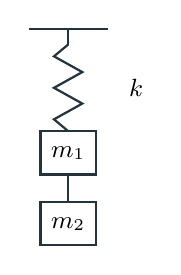
\begin{tikzpicture}
\draw[object] (-.5,3)--(.5,3);\draw[object] (0,3)--(0,2.8);
\draw[object] (0,2.8)--(-.18,2.65)--(.18,2.45)--(-.18,2.25)--(.18,2.05)--(-.18,1.85)--(0,1.7);
\filldraw[object,fill=white] (-.35,1.15) rectangle (.35,1.7);\node at (0,1.42) {$m_1$};\draw[object] (0,1.15)--(0,.8);\filldraw[object,fill=white] (-.35,.25) rectangle (.35,.8);\node at (0,.52) {$m_2$};\node[right] at (.65,2.25) {$k$};
\end{tikzpicture}
\figcaption{图 3.1\quad 撤去下挂物前的平衡状态。}
\end{minipage}\end{center}

\Needspace{5\baselineskip}

\pdfbookmark[3]{题型定位}{q1-h0}

\subsection*{题型定位}

竖直弹簧撤去下挂物后的振动。重力与弹性势能共同确定新的势能最低点，初始位置相对这个点的偏移决定最大速率。

\Needspace{5\baselineskip}

\pdfbookmark[3]{知识点}{q1-h1}

\subsection*{知识点}

撤去时位置和速度连续，平衡位置与振动质量改变。将弹性势能与重力势能配方后，得到以新平衡点为中心的抛物线；其初始高度差转化为最大动能。


\Needspace{5\baselineskip}

\pdfbookmark[3]{物理图像}{q1-h2}

\subsection*{物理图像}

撤去前的平衡伸长由 $(m_1+m_2)g$ 决定。撤去瞬间伸长量保持原值，向上的弹力大于 $m_1g$，物体先向上加速。解图3.1A 的两条平衡线相差 $m_2g/k$，首次经过上方的新平衡线时向上速率最大。

\Needspace{5\baselineskip}

\pdfbookmark[3]{解题入口}{q1-h3}

\subsection*{解题入口}

取图3.1A 向下的 $x$ 轴，先写
\[
x_i=\frac{(m_1+m_2)g}{k},\qquad x_e=\frac{m_1g}{k}.
\]
以 $\xi=x-x_e$ 配方 $U=\tfrac12k\xi^2-\tfrac12kx_e^2$，初值为 $\xi(0)=m_2g/k,\dot\xi(0)=0$。经过 $\xi=0$ 时，振动势能全部变为动能。

\Needspace{5\baselineskip}

\pdfbookmark[3]{标准解法}{q1-h4}

\subsection*{标准解法}

以弹簧原长时 $m_1$ 的位置为原点，竖直向下为 $x$ 正方向。解图3.1A 上方的虚线是撤去下挂物后的平衡位置 $x_e$，下方的虚线是释放位置 $x_i$。物体从静止出发，两条线的距离就是这次振动的振幅。
\begin{center}\begin{minipage}{\linewidth}\centering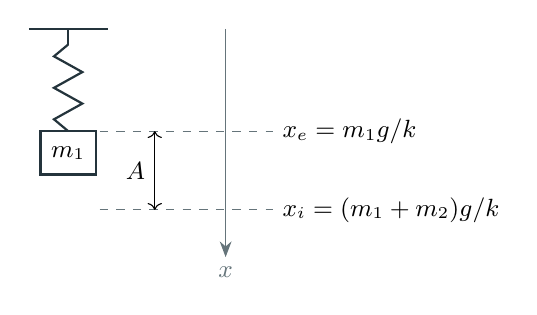
\begin{tikzpicture}
\draw[object] (-.5,3)--(.5,3);\draw[object] (0,3)--(0,2.8);
\draw[object] (0,2.8)--(-.18,2.65)--(.18,2.45)--(-.18,2.25)--(.18,2.05)--(-.18,1.85)--(0,1.7);
\filldraw[object,fill=white] (-.35,1.15) rectangle (.35,1.7);\node at (0,1.42) {$m_1$};\draw[axis] (2,3)--(2,.1) node[below] {$x$};\draw[guide] (.4,1.7)--(2.6,1.7);\draw[guide] (.4,.7)--(2.6,.7);
\node[right] at (2.6,1.7) {$x_e=m_1g/k$};\node[right] at (2.6,.7) {$x_i=(m_1+m_2)g/k$};\draw[<->] (1.1,.7)--(1.1,1.7) node[midway,left] {$A$};
\end{tikzpicture}
\figcaption{解图 3.1A\quad 从 $x_i$ 静止释放后，首次到 $x_e$ 时向上速率最大。}
\end{minipage}\end{center}

\subsubsection*{平衡位置与释放状态}
撤去下挂物之前，弹簧所承受的总重力为 $(m_1+m_2)g$，故伸长量
\[
x_i=\frac{(m_1+m_2)g}{k}.
\]
撤去过程不给冲量，所以撤去后的瞬间位置仍为 $x_i$，速度仍为零。此后参加运动的物体只有 $m_1$，新的平衡条件是 $kx_e=m_1g$，因而
\[
x_e=\frac{m_1g}{k},\qquad x_i-x_e=\frac{m_2g}{k}.
\]
解图 3.1A 中两条水平虚线之间的距离是相对新平衡位置的初位移。弹簧刚开始收缩时，弹力比 $m_1g$ 大 $m_2g$，所以 $m_1$ 先向上运动。

\subsubsection*{速度最大的位置}
撤去后的运动方程是 $m_1\ddot x=m_1g-kx$。令 $\xi=x-x_e$，便有
\[
\ddot\xi+\frac{k}{m_1}\xi=0.
\]
从 $x_i$ 上行到 $x_e$ 时，$\xi>0$，加速度向上，上行速率增加。越过 $x_e$ 后，$\xi<0$，加速度向下，上行速率减小。因而首次经过 $x_e$ 时速率最大。振动的最上端为 $x_e-A=(m_1-m_2)g/k$。$m_2\ge m_1$ 时物体能到弹簧原长处，那里弹力为零，加速度为向下的 $g$。

取物体、弹簧和地球为系统，势能可配方为
\[
U(x)=\frac12kx^2-m_1gx
=\frac12k(x-x_e)^2-\frac12kx_e^2.
\]
把释放位置代入同一势能式，可以把振动能量中的各项展开。初始速度为零，故释放瞬间的机械能为
\[
E=\frac12kx_i^2-m_1gx_i
=\frac{(m_1+m_2)^2g^2}{2k}
-\frac{m_1(m_1+m_2)g^2}{k}
=\frac{m_2^2-m_1^2}{2k}g^2,
\]
最小势能为 $U_{\min}=-m_1^2g^2/(2k)$。相减后留下 $m_2^2g^2/(2k)$，与配方中相对平衡位置的振动能量相同。
从释放点到新平衡位置，势能差全部转成动能：
\[
\frac12m_1v_{\max}^2
 =\frac12k(x_i-x_e)^2
 =\frac{m_2^2g^2}{2k}.
\]
所以
\[
\boxed{v_{\max}=\frac{m_2g}{\sqrt{m_1k}}}.
\]
简谐运动的角频率为 $\omega=\sqrt{k/m_1}$，速度幅值为 $\omega A$。从图3.1A 的 $x_i$ 到 $x_e$ 对应四分之一周期。当 $m_2\to0$ 时，两条平衡线靠拢，振幅和最大速率均趋零。
图3.1A 中实线方块在 $x_e$。第一次经过时速度为 $-v_{\max}$。由 $U'(x_e)=kx_e-m_1g=0$、$U''(x_e)=k>0$，也可看出这里是总势能唯一的最低点。撤去操作给出了 $x(0)=x_i,\dot x(0)=0$；此后的能量方程用留下的物体、弹簧和地球组成系统。


\Needspace{5\baselineskip}

\pdfbookmark[3]{关键洞察}{q1-h5}

\subsection*{关键洞察}

初始弹簧伸长包含两块的总重量，新平衡伸长只含留下的 $m_1$。两者的差是振幅。能量差用撤去后系统的势能计算。

\Needspace{5\baselineskip}

\pdfbookmark[3]{易错点}{q1-h6}

\subsection*{易错点}

\begin{itemize}
\item 新平衡条件为 $kx_e=m_1g$，最大速率在 $x_e$ 处取得。
\item 撤去后的惯性质量为 $m_1$，重力势能为 $-m_1gx$。
\item 第一次经过新平衡点时速度向上；以向下为正，它的速度为负，速率为正。
\end{itemize}

\Needspace{5\baselineskip}

\pdfbookmark[3]{课堂讲解建议}{q1-h7}

\subsection*{课堂讲解建议}

先请学生在解图3.1A 标出 $x_i$ 与 $x_e$，指出撤去瞬间弹力与留下物体重力相差 $m_2g$，于是加速度向上。再让学生比较振幅 $A$ 与平衡伸长 $x_e$。若 $A\ge x_e$，物体能到原长点，那里的加速度向下。请学生分别说明原长点与新平衡点的合力。最后把 $m_2$ 逐渐减到零，让学生同时描述图中两条线的距离和最大速率的变化。

\Needspace{5\baselineskip}

\pdfbookmark[3]{变式训练}{q1-h8}

\subsection*{变式训练}

\begin{enumerate}
\item 交换两物体的上下位置，再撤去下方的 $m_1$，求留下的 $m_2$ 的最大速率。撤去过程仍不给冲量，初始伸长为 $(m_1+m_2)g/k$，新平衡伸长为 $m_2g/k$。两者相差 $A_1=m_1g/k$。变图3.1V1 以新平衡点计位移，振动势能为 $U_{\rm osc}=k\xi^2/2$，初始振动能量为 $E_1=kA_1^2/2$。到抛物线最低点时，
\[
\frac12m_2v_{\max}^2=\frac12kA_1^2,\qquad
v_{\max}=\frac{m_1g}{\sqrt{m_2k}}.
\]
\begin{center}\begin{minipage}{.98\linewidth}\centering
\begin{tikzpicture}[scale=.88,transform shape]
\draw[axis] (-2.6,0)--(2.8,0) node[right] {$\xi/A_1$};
\draw[axis] (0,0)--(0,2.95) node[above] {$U_{\rm osc}/E_1$};
\draw[traj,domain=-1.13:1.13,samples=90] plot ({2*\x},{2*\x*\x});
\draw[guide] (-2,2)--(2.5,2) node[right] {$E_{\rm osc}/E_1=1$};
\fill[accent] (2,2) circle(1.65pt) node[above right] {释放点};
\fill[accent] (0,0) circle(1.65pt);
\draw[force] (0,2)--(0,0) node[midway,left] {$K_{\max}/E_1$};
\node[below] at (2,0) {$1$};
\end{tikzpicture}
\figcaption{变图3.1V1\quad 留下 $m_2$ 时，以新平衡位置为零位移，释放点的振动势能变为最大动能。}
\end{minipage}\end{center}
\item 撤去 $m_2$ 后，振幅和首次到达新平衡点的时间是多少？令 $\omega=\sqrt{k/m_1}$，相对新平衡点的初位移为 $A=m_2g/k$，初速度为零，故 $\xi=A\cos\omega t$、$v=-\omega A\sin\omega t$。变图3.1V2 中，位移线第一次过横轴时 $\omega t=\pi/2$。此时归一化速度为 $-1$，物体正以最大速率上行。所以振幅为 $A$，首次到达时间为
\[
t=\frac{\pi}{2\omega}=\frac\pi2\sqrt{\frac{m_1}{k}}.
\]
\begin{center}\begin{minipage}{.98\linewidth}\centering
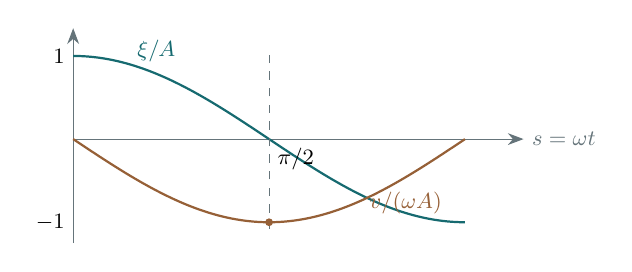
\begin{tikzpicture}[scale=.88,transform shape]
\draw[axis] (0,0)--(6.5,0) node[right] {$s=\omega t$};
\draw[axis] (0,-1.5)--(0,1.6);
\draw[traj,domain=0:3.14159,samples=90] plot ({1.8*\x},{1.2*cos(deg(\x))});
\draw[thick,color=warm,domain=0:3.14159,samples=90] plot ({1.8*\x},{-1.2*sin(deg(\x))});
\draw[guide] ({.9*pi},-1.3)--({.9*pi},1.3);
\node[below right] at ({.9*pi},0) {$\pi/2$};
\node[above,text=accent] at (1.2,.99) {$\xi/A$};
\node[below,text=warm] at (4.8,-.64) {$v/(\omega A)$};
\node[left] at (0,1.2) {$1$};\node[left] at (0,-1.2) {$-1$};
\fill[warm] ({.9*pi},-1.2) circle(1.6pt);
\end{tikzpicture}
\figcaption{变图3.1V2\quad 位移首次过零时，有符号速度达到负的极值。}
\end{minipage}\end{center}
\item 用简谐运动求最大速率，并允许撤去时另给向下初速度 $u$。运动方程仍为 $\ddot\xi+\omega^2\xi=0$，初值为 $\xi(0)=A,\dot\xi(0)=u$，于是
\[
\xi=A\cos\omega t+\frac u\omega\sin\omega t,\qquad
v=-\omega A\sin\omega t+u\cos\omega t.
\]
平方相加得到 $(\xi/A)^2+[v/(\omega A)]^2=1+[u/(\omega A)]^2$。变图3.1V3 取 $u=3\omega A/4$，初态为 $(1,3/4)$，相轨道半径为 $5/4$，纵轴两端的速度大小相同。一般情况下，
\[
v_{\max}=\sqrt{u^2+\omega^2A^2}
=\sqrt{u^2+\frac{m_2^2g^2}{m_1k}}.
\]
令 $u=0$，就得到 $\omega A=m_2g/\sqrt{m_1k}$。
\begin{center}\begin{minipage}{.98\linewidth}\centering
\begin{tikzpicture}[scale=.88,transform shape]
\draw[axis] (-2.9,0)--(3.05,0) node[right] {$\xi/A$};
\draw[axis] (0,-2.75)--(0,2.9) node[above] {$v/(\omega A)$};
\draw[traj] (0,0) circle(2.25);
\coordinate (P) at (1.8,1.35);
\fill[accent] (P) circle(1.8pt) node[above right] {初态 $(1,3/4)$};
\draw[motion] (P) arc(36.8699:10:2.25);
\draw[guide] (1.8,0)--(P)--(0,1.35);
\fill[warm] (0,2.25) circle(1.65pt) node[left] {$5/4$};
\fill[warm] (0,-2.25) circle(1.65pt) node[left] {$-5/4$};
\node[below] at (1.8,0) {$1$};
\end{tikzpicture}
\figcaption{变图3.1V3\quad 初速度非零时，初态在更大的相轨道上，经过零位移处取得最大速率。}
\end{minipage}\end{center}
\end{enumerate}

\clearpage

\pdfbookmark[2]{第 2 题 带摩擦水平弹簧振子的过原点条件}{q2}

\section*{第 2 题\quad 带摩擦水平弹簧振子的过原点条件}

\tagline{M-03-02}

水平轻弹簧一端固定，另一端连接质量为 $m$ 的小球，劲度系数为 $k$。小球在粗糙水平面上运动，静、动摩擦系数均为 $\mu$。弹簧原长位置为 $O$。从右侧 $OA=l_0$ 的 $A$ 点静止释放。
\begin{enumerate}\item 为使小球穿过 $O$ 且只穿过一次，$\mu$ 应取什么范围？以速度不为零并越到另一侧为“穿过”。\item 若还要求小球在左侧第一个转折点 $B$ 永久停住，$OB=l_1$ 的最大值是多少？\end{enumerate}

\begin{center}\begin{minipage}{\linewidth}\centering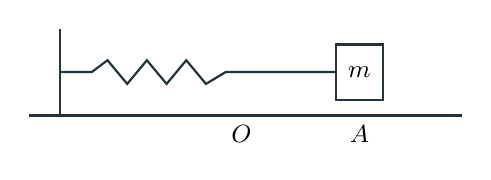
\begin{tikzpicture}
\draw[object] (-.4,0)--(5.1,0);\draw[object] (0,0)--(0,1.1);\draw[object] (0,.55)--(.4,.55)--(.6,.7)--(.85,.4)--(1.1,.7)--(1.35,.4)--(1.6,.7)--(1.85,.4)--(2.1,.55)--(3.5,.55);\filldraw[object,fill=white] (3.5,.2) rectangle (4.1,.9);\node at (3.8,.55) {$m$};\node[below] at (2.3,0) {$O$};\node[below] at (3.8,0) {$A$};
\end{tikzpicture}
\figcaption{图 3.2\quad 小球从伸长位置释放，摩擦始终反向于运动。}
\end{minipage}\end{center}

\Needspace{5\baselineskip}

\pdfbookmark[3]{题型定位}{q2-h0}

\subsection*{题型定位}

有干摩擦的水平弹簧运动。每段路程的摩擦耗能决定能否越过原点，转折点的静摩擦条件决定球是否启动下一段运动。

\Needspace{5\baselineskip}

\pdfbookmark[3]{知识点}{q2-h1}

\subsection*{知识点}

弹簧势能、滑动摩擦功、静摩擦平衡与分段能量关系。穿过原点要求到达该处时有正动能；速度降到零后，按当地弹力与最大静摩擦比较，决定后续运动。


\Needspace{5\baselineskip}

\pdfbookmark[3]{物理图像}{q2-h2}

\subsection*{物理图像}

解图3.2A 取右侧释放点 $A$、原长点 $O$ 和第一次左侧停点 $B$。从 $A$ 向左滑动时摩擦向右，弹簧从伸长转为压缩。到 $B$ 速度为零后，只有 $kl_1>\mu mg$ 时才向右启动，这时滑动摩擦改向左。

\Needspace{5\baselineskip}

\pdfbookmark[3]{解题入口}{q2-h3}

\subsection*{解题入口}

先把弹力与摩擦的比较写成长度 $d=\mu mg/k$。第一次到达 $O$ 的动能与首次左转折量为
\[
K_O=\frac{k l_0}{2}(l_0-2d),\qquad l_1=l_0-2d.
\]
先由 $K_O>0$ 保证首次穿过，再在 $B$ 比较 $l_1$ 与 $d$。若 $l_1>d$，返回到 $O$ 的动能由 $K'_O=k l_1(l_1-2d)/2$ 决定。

\Needspace{5\baselineskip}

\pdfbookmark[3]{标准解法}{q2-h4}

\subsection*{标准解法}

记 $d=\mu mg/k$，它是最大静摩擦能够平衡的弹簧伸长或压缩量。解图3.2A 中，球首次向左越过 $O$ 后在 $B$ 点停下。弹力若大于最大静摩擦，球便向右返回；若返回时动能先耗尽，它会在 $O$ 左侧再次停下。
\begin{center}\begin{minipage}{\linewidth}\centering\begin{tikzpicture}
\draw[axis] (-2.3,0)--(2.6,0) node[right] {$x$};\foreach \x/\lab in {-1.2/B,0/O,2/A}{\fill (\x,0) circle(2pt);\node[below] at (\x,0) {$\lab$};}
\draw[motion] (1.8,.5)--(-1,.5) node[midway,above] {第一次向左};\draw[motion] (-1,-.7)--(-.2,-.7) node[midway,below] {可能返回};\node at (-1.2,1.2) {$-l_1$};\node at (2,1.2) {$l_0$};
\end{tikzpicture}
\figcaption{解图 3.2A\quad 穿过原点与在首个转折点永久停住是两个条件。}
\end{minipage}\end{center}

\subsubsection*{首次穿过与左侧转折点}
设 $x$ 向右为正，并记 $d=\mu mg/k$。当 $kl_0\leq\mu mg$ 时，$A$ 点的弹力可以由静摩擦平衡，球保持静止。要从 $A$ 启动，需有 $l_0>d$，随后再根据到 $O$ 的动能判断是否穿过。
从 $A$ 向左到 $O$，摩擦力向右，所做的功为 $-\mu mgl_0$。到达 $O$ 的动能为
\[
K_O=\frac12kl_0^2-\mu mgl_0
 =\frac{k l_0}{2}(l_0-2d).
\]
“穿过”要求 $K_O>0$，即 $d<l_0/2$。这个条件也自动保证球能从 $A$ 开始运动。

设首次在左侧停下的位置为 $x=-l_1$，如解图 3.2A。此段总路程为 $l_0+l_1$，两端速度都为零，因此
\[
\frac12kl_0^2-\mu mg(l_0+l_1)=\frac12kl_1^2.
\]
分解平方差并约去正数 $l_0+l_1$，得到
\[
\boxed{l_1=l_0-2d}.
\]

\subsubsection*{转折后会不会再穿过}
在 $B$ 点，弹簧力向右，大小为 $kl_1$。若 $l_1\leq d$，静摩擦足以平衡弹力，小球永久留在 $B$。若 $l_1>d$，球向右运动，摩擦随之改向左。
后一种情况下，由 $B$ 返回 $O$ 的动能为
\[
K'_O=\frac12kl_1^2-\mu mgl_1
=\frac{k l_1}{2}(l_1-2d).
\]
只有 $l_1>2d$ 才能第二次穿过；$l_1=2d$ 时恰好停在 $O$；$d<l_1<2d$ 时在 $O$ 左侧停下。此时剩余压缩量 $2d-l_1<d$，静摩擦能将球留住，不会再开始新的往返。

所以“不再穿过”的统一条件是 $l_1\leq2d$，与首次穿过的条件联立：
\[
l_0-2d\leq2d,\qquad d<l_0/2.
\]
得
\[
\boxed{\frac{kl_0}{4mg}\leq\mu<\frac{kl_0}{2mg}}.
\]
取下界时，球返回到 $O$ 恰好速度为零，故只计第一次穿过。取上界时，首次到达 $O$ 就停下，穿过次数为零，因此上界是开端点。

\subsubsection*{首个转折点永久停住}
第二问要求第一次在 $B$ 停下后就保持静止，对应弹力 $kl_1$ 由最大为 $kd$ 的静摩擦平衡，即 $l_1\leq d$。代入 $d=(l_0-l_1)/2$，得 $3l_1\leq l_0$。于是
\[
\boxed{l_{1,\max}=\frac{l_0}{3}},\qquad
\boxed{\mu=\frac{kl_0}{3mg}}.
\]
整个一次穿过区间可以进一步分成两段：$l_0/4\leq d<l_0/3$ 时球会返回，但不再穿过；$l_0/3\leq d<l_0/2$ 时球留在第一个左侧转折点。
\subsubsection*{用往返路程计算摩擦耗能}
图3.2A 给出从 $A$ 到 $B$ 再返回的路线。能从 $B$ 启动时，沿这一路线累加摩擦功。
若小球从$B$启动返回，累计走到$O$的路程是$l_0+2l_1$，
这一路程所需的摩擦耗能为$\mu mg(l_0+2l_1)$。
不再穿过$O$要求候选返回动能不大于零，即
\[
\frac12kl_0^2-\mu mg(l_0+2l_1)\leq0.
\]
在已经确认返回会启动的分支中，这个不等式的等号表示恰好到$O$停住。
若球已留在$B$，这段返回路程并未发生，应使用前面的静摩擦判断；
它与上述分支最后给出同一个一次穿过区间。
代入$l_1=l_0-2\mu mg/k$，逐项整理为
\[
\begin{aligned}
&\frac{4m^2g^2}{k}\mu^2-3mgl_0\mu+\frac12kl_0^2\leq0,\\
&\frac{4m^2g^2}{k}
\left(\mu-\frac{kl_0}{4mg}\right)
\left(\mu-\frac{kl_0}{2mg}\right)\leq0.
\end{aligned}
\]
首项系数为正，故二次式在两根之间非正。
再与首次穿过所需的 $\mu<kl_0/(2mg)$ 相交，得到前面的左闭右开区间。左端对应返回到 $O$ 时动能为零，右端对应第一次到 $O$ 时动能为零，两个端点的运动不同。

返回却未过$O$时，还能求出最终位置。
记最终压缩量为$l_2\geq0$，从$B$到此处的路程是$l_1-l_2$，于是
\[
\frac12kl_1^2-\mu mg(l_1-l_2)=\frac12kl_2^2,
\qquad l_2=2d-l_1=4d-l_0.
\]
在$l_0/4\leq d<l_0/3$内，$0\leq l_2<d$，静摩擦能维持最后的停止。
球第二次停下的位置为 $x=-l_2$。由于 $l_2<l_1$，它已从第一次停下的位置 $x=-l_1$ 向右移动了一段。
解图3.2B用同一条$d/l_0$轴归纳各段过程：
能否启动、能否首次穿过、是否返回、返回后能否再穿过，需要按这个顺序判断。
\begin{center}\begin{minipage}{\linewidth}\centering
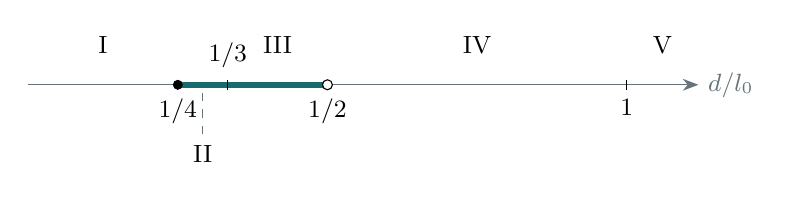
\begin{tikzpicture}[x=7.6cm]
\draw[axis] (0,0)--(1.12,0) node[right] {$d/l_0$};
\draw[traj,line width=2pt] (.25,0)--(.5,0);
\foreach \x/\lab in {.25/{1/4},.5/{1/2},1/{1}}{
 \draw (\x,-.06)--(\x,.06);\node[below] at (\x,-.06) {$\lab$};}
\draw (.333333,-.06)--(.333333,.06);\node[above] at (.333333,.09) {$1/3$};
\fill (.25,0) circle(1.8pt);\draw[fill=white] (.5,0) circle(1.8pt);
\node at (.125,.5) {I};\node at (.416667,.5) {III};
\node at (.75,.5) {IV};\node at (1.06,.5) {V};
\draw[guide] (.291667,-.1)--(.291667,-.65);\node[below] at (.291667,-.65) {II};
\end{tikzpicture}

\smallskip
\begin{tabular}{@{}cll@{}}
I & $0<d/l_0<1/4$ & 至少再次穿过\\
II & $1/4\leq d/l_0<1/3$ & 返回，但不再穿过\\
III & $1/3\leq d/l_0<1/2$ & 留在首个左转折点\\
IV & $1/2\leq d/l_0<1$ & 到不了左侧\\
V & $d/l_0\geq1$ & 可由静摩擦留在释放点
\end{tabular}
\figcaption{解图3.2B\quad 加粗区间为一次穿过；$d=0$时无摩擦，会持续往复穿过。}
\end{minipage}\end{center}


\Needspace{5\baselineskip}

\pdfbookmark[3]{关键洞察}{q2-h5}

\subsection*{关键洞察}

首次穿过以后，还要区分在左侧停住与启动返回。若 $l_1\leq d$，球留在 $B$。若 $d<l_1\leq 2d$，球返回但至多回到 $O$，两段参数都给一次穿过。

\Needspace{5\baselineskip}

\pdfbookmark[3]{易错点}{q2-h6}

\subsection*{易错点}

\begin{itemize}
\item 第一次到 $O$ 时 $K_O>0$ 才计为穿过，等于零时在 $O$ 停下。
\item 从 $B$ 返回以前，先比较 $kl_1$ 与最大静摩擦；启动后摩擦才改向左。
\item 每段摩擦功按实际路程计算，返回时仍持续耗能。
\item 在 $B$ 永久停住的条件为 $l_1\leq d$，它与仅要求不再穿过 $O$ 的条件不同。
\end{itemize}

\Needspace{5\baselineskip}

\pdfbookmark[3]{课堂讲解建议}{q2-h7}

\subsection*{课堂讲解建议}

先让学生沿解图3.2A 说出 $A\to O$、$O\to B$ 两段摩擦的方向和路程。到 $B$ 时把速度箭头擦去，问“弹簧力是否已经足够使球返回？”由 $l_1$ 与 $d$ 的比较回答。再依次取 $d/l_0=1/4,1/3,1/2$，请学生描述返回恰到原点、首个转折点恰能静止、第一次恰到原点这三种运动。

\Needspace{5\baselineskip}

\pdfbookmark[3]{变式训练}{q2-h8}

\subsection*{变式训练}

\begin{enumerate}
\item 要求第一次恰好停在 $O$，求 $\mu$。从 $A$ 到 $O$，初始势能全部被摩擦耗散，
\[
\frac12kl_0^2=\mu mgl_0,\qquad \mu=\frac{kl_0}{2mg}.
\]
此时 $d=l_0/2<l_0$，球能够从 $A$ 启动。变图3.2V1 用 $s=x/l_0$ 和 $E_0=kl_0^2/2$ 表示途中动能，$K/E_0=s-s^2$ 在 $0<s<1$ 为正，到 $O$ 时降到零。球到达原点就停下，穿过次数为零。
\begin{center}\begin{minipage}{.98\linewidth}\centering
\begin{tikzpicture}[scale=.88,transform shape]
\draw[axis] (0,0)--(5.55,0) node[right] {$s=x/l_0$};
\draw[axis] (0,0)--(0,2.1) node[above] {$K/E_0$};
\draw[traj,domain=0:1,samples=90] plot ({4.7*\x},{6*(\x-\x*\x)});
\fill[accent] (0,0) circle(1.7pt) node[below] {$O$};
\fill[accent] (4.7,0) circle(1.7pt) node[below] {$A,\ 1$};
\draw[guide] (2.35,0)--(2.35,1.5);
\node[left] at (0,1.5) {$1/4$};
\draw[motion] (4.2,-.65)--(.5,-.65) node[midway,below] {从 $A$ 到 $O$};
\end{tikzpicture}
\figcaption{变图3.2V1\quad 取 $d=l_0/2$，球在两端的动能都为零，中间运动时动能为正。}
\end{minipage}\end{center}
\item 要求只穿过两次而不穿过第三次，求 $\mu$ 的范围。首次左转折量为 $l_1=l_0-2d$。能第二次穿过要求 $l_1>2d$，即 $d<l_0/4$；随后右转折量为 $l_2=l_1-2d=l_0-4d$。在右转折点，若 $l_2\leq d$，球直接停住；若 $l_2>d$，它向左返回，而第三次穿过要求 $l_2>2d$。合并这两种不再穿过的情况，得 $l_2\leq2d$，因此
\[
\frac{l_0}{6}\leq d<\frac{l_0}{4},
\qquad \frac{kl_0}{6mg}\leq\mu<\frac{kl_0}{4mg}.
\]
变图3.2V2 取 $d=l_0/5$，两次穿过以后到 $C$，此处 $l_2=d$，最大静摩擦恰能维持静止。在下端 $d=l_0/6$，第三次只到达 $O$ 并停下，故包含等号。
\begin{center}\begin{minipage}{.98\linewidth}\centering
\begin{tikzpicture}[scale=.88,transform shape]
\draw[axis] (-2.9,0)--(4.8,0) node[right] {$x/l_0$};
\foreach \x/\lab in {-2.4/{B,\ -3/5},0/O,.8/{C,\ 1/5},4/{A,\ 1}}{
\fill (\x,0) circle(1.6pt) node[below=3pt] {$\lab$};}
\draw[motion] (4,.65)--(-2.4,.65) node[midway,above] {第一次穿过};
\draw[motion] (-2.4,1.55)--(.8,1.55) node[midway,above] {第二次穿过};
\draw[guide] (-2.4,0)--(-2.4,1.55);
\draw[guide] (.8,0)--(.8,1.55);
\node[right] at (1.3,-.85) {$d/l_0=1/5$};
\end{tikzpicture}
\figcaption{变图3.2V2\quad 一次左行、一次右行后到达 $C$，此处弹力恰可由静摩擦维持。}
\end{minipage}\end{center}
\item 只有 $O$ 左侧粗糙，右侧光滑，求只穿过一次及首个转折点停住的条件。第一次到 $O$ 的动能为 $kl_0^2/2>0$。从 $O$ 进入粗糙区，摩擦耗能为 $kd\,l_1$，所以
\[
l_1^2+2dl_1=l_0^2,\qquad l_1=\sqrt{d^2+l_0^2}-d.
\]
变图3.2V3 的蓝线是 $l_1/l_0$，它与虚线 $2d/l_0$ 的交点给出 $l_1\leq2d$ 的阈值。这意味着从左侧返回时至多到达 $O$，故只穿过一次的条件为 $d\geq l_0/(2\sqrt2)$，范围没有有限上端。若要求在首个左转折点停住，还需 $l_1\leq d$，由蓝线与红线的交点得到 $d\geq l_0/\sqrt3$。在两个阈值之间，球会向右启动，继而仍在左侧停下，最终压缩量为
\[
l_2=2d-l_1=3d-\sqrt{d^2+l_0^2},\qquad 0\leq l_2<d.
\]
静摩擦能维持这个位置。较小阈值的等号对应返回恰到 $O$，较大阈值的等号对应首个转折点恰可静止。
\begin{center}\begin{minipage}{.98\linewidth}\centering
\begin{tikzpicture}[scale=.88,transform shape]
\draw[axis] (0,0)--(6.2,0) node[right] {$r=d/l_0$};
\draw[axis] (0,0)--(0,3.9) node[above] {长度与 $l_0$ 的比};
\draw[traj,domain=0:.9,samples=100] plot ({6*\x},{2*(sqrt(1+\x*\x)-\x)});
\draw[thick,color=warm,domain=0:.9] plot ({6*\x},{2*\x});
\draw[guide,domain=0:.9] plot ({6*\x},{4*\x});
\coordinate (L) at ({3/sqrt(2)},{sqrt(2)});
\coordinate (U) at ({6/sqrt(3)},{2/sqrt(3)});
\fill[accent] (L) circle(1.7pt);
\fill[accent] (U) circle(1.7pt);
\draw[guide] (L)--({3/sqrt(2)},0) node[below] {$1/(2\sqrt2)$};
\draw[guide] (U)--({6/sqrt(3)},0) node[below] {$1/\sqrt3$};
\node[above right,text=accent] at (4.5,1.0) {$l_1/l_0$};
\node[above,text=warm] at (4.55,1.65) {$r$};
\node[above] at (4.5,3) {$2r$};
\end{tikzpicture}
\figcaption{变图3.2V3\quad 左转折压缩量与 $2d$、$d$ 分别相交，给出不再穿过和直接停住的阈值。}
\end{minipage}\end{center}
\end{enumerate}

\clearpage

\pdfbookmark[2]{第 3 题 斜面摩擦中动能等于势能的位置}{q3}

\section*{第 3 题\quad 斜面摩擦中动能等于势能的位置}

\tagline{M-03-03}

木块沿倾角 $\theta=30^\circ$ 的足够长斜面，以 $v_0=4.5\,\mathrm{m/s}$ 的初速度上滑。静、动摩擦系数均为 $\mu=0.35$。以初始位置为重力势能零点，求动能等于重力势能时相对初始位置的高度。取 $g=10\,\mathrm{m/s^2}$。

\begin{center}\begin{minipage}{\linewidth}\centering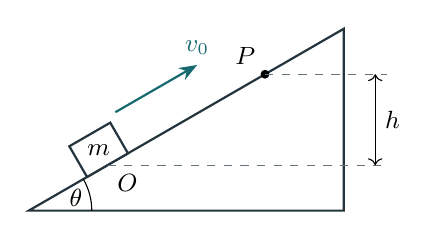
\begin{tikzpicture}
\draw[object] (0,0)--(4,2.309401)--(4,0)--cycle;
\filldraw[object,fill=white,rotate around={30:(1,.57735)}] (.7,.57735) rectangle (1.3,1.02735);
\node at (.8875,.772206) {$m$};\node[below right] at (1,.57735) {$O$};
\draw[motion] (1.1,1.25)--(2.13923,1.85) node[above] {$v_0$};
\draw (.8,0) arc(0:30:.8);\node at (.6,.16) {$\theta$};
\fill (3,1.732051) circle(1.6pt);\node[above left] at (3,1.732051) {$P$};
\draw[guide] (1,.57735)--(4.55,.57735);\draw[guide] (3,1.732051)--(4.55,1.732051);
\draw[<->] (4.4,.57735)--(4.4,1.732051) node[midway,right] {$h$};
\end{tikzpicture}
\figcaption{图 3.3\quad 从初始位置$O$量取竖直高度$h$，$P$表示上滑途中的位置。}
\end{minipage}\end{center}

\Needspace{5\baselineskip}

\pdfbookmark[3]{题型定位}{q3-h0}

\subsection*{题型定位}

沿粗糙斜面往返运动的功能关系。分别求上滑和下滑的动能随高度的变化，再与同一个重力势能函数相交，确定两个运动阶段的相等位置。

\Needspace{5\baselineskip}

\pdfbookmark[3]{知识点}{q3-h1}

\subsection*{知识点}

重力功与竖直高度、摩擦功与沿面路程、最高点的静摩擦条件、统一的势能零点。经过同一高度时，两次的重力势能相同，动能因摩擦累计耗能不同而不同。


\Needspace{5\baselineskip}

\pdfbookmark[3]{物理图像}{q3-h2}

\subsection*{物理图像}

解图3.3A 中，上滑箭头从 $O$ 指向最高点 $H$，下滑箭头从 $H$ 返回。解图3.3B 把这两次运动的动能分成两条直线，重力势能随 $h$ 增加。下滑支的动能在同一高度更低，因此第二个交点低于第一个。

\Needspace{5\baselineskip}

\pdfbookmark[3]{解题入口}{q3-h3}

\subsection*{解题入口}

记 $q=\mu\cot\theta$、$K_0=mv_0^2/2$。先由 $K_{\uparrow}=K_0-mg(1+q)h$ 求上滑交点 $h_1$ 和最高点 $H$。在最高点比较重力沿面分量与最大静摩擦，确认能下滑后，再用 $K_{\downarrow}=mg(1-q)(H-h)$ 求第二个交点 $h_2$。

\Needspace{5\baselineskip}

\pdfbookmark[3]{标准解法}{q3-h4}

\subsection*{标准解法}

解图3.3A 以初始点 $O$ 为高度零点。上滑从 $O$ 到 $h$，路程为 $h/\sin\theta$；下滑从最高点 $H$ 到 $h$，这段路程为 $(H-h)/\sin\theta$。两段中摩擦始终反向于运动，所做的功均为负。
\begin{center}\begin{minipage}{\linewidth}\centering\begin{tikzpicture}
\draw[axis] (0,-.2)--(0,3.2) node[above] {$h$};\foreach \y/\lab in {0/0,.8/h_2,1.7/h_1,2.7/H}{\draw (-.1,\y)--(.1,\y);\node[left] at (0,\y) {$\lab$};}\draw[motion] (1,.1)--(1,2.6) node[midway,right] {上滑};\draw[motion] (2.6,2.6)--(2.6,.1) node[midway,right] {下滑};\node[anchor=west,align=left] at (3.65,1.4) {$K_{\uparrow}=K_0-mg(1+\mu\cot\theta)h$\\$K_{\downarrow}=mg(1-\mu\cot\theta)(H-h)$};
\end{tikzpicture}
\figcaption{解图 3.3A\quad 同一高度处，上滑和下滑的动能不同。}
\end{minipage}\end{center}

\subsubsection*{上滑段}
设相对初始位置的竖直高度为 $h$，斜面路程为 $h/\sin\theta$。支持力为 $mg\cos\theta$，摩擦做功为
\[
W_f=-\mu mg\cos\theta\,\frac{h}{\sin\theta}
=-\mu mgh\cot\theta.
\]
记 $q=\mu\cot\theta$、$K_0=mv_0^2/2$。由动能定理，
\[
K_{\uparrow}(h)=K_0-mg(1+q)h.
\]
重力势能为 $U_g=mgh$，令两者相等，得到
\[
\boxed{h_1=\frac{v_0^2}{2g(2+q)}}.
\]
最高点由 $K_{\uparrow}(H)=0$ 确定，
\[
H=\frac{v_0^2}{2g(1+q)}.
\]
由于 $2+q>1+q$，可知 $0<h_1<H$，上滑过程中确实经过这一高度。

\subsubsection*{最高点能否返回}
木块停在最高点时，沿斜面向下的重力分量为 $mg\sin\theta$，最大静摩擦为 $\mu mg\cos\theta$。本题 $\mu=0.35<\tan30^\circ$，静摩擦不足以留住木块，所以还应计算下滑段。

从最高点下降至高度 $h$，路程为 $(H-h)/\sin\theta$。重力做正功、摩擦做负功，因而
\[
K_{\downarrow}(h)=mg(H-h)-\mu mg(H-h)\cot\theta
=mg(1-q)(H-h).
\]
令 $K_{\downarrow}(h_2)=mgh_2$，逐项移项：
\[
(1-q)H-(1-q)h_2=h_2,\qquad
\boxed{h_2=\frac{1-q}{2-q}H}.
\]

\subsubsection*{两个高度及其顺序}
$q=0.35\sqrt3\approx0.6062$，所以
\[
H\approx0.630\,\mathrm m,\quad
\boxed{h_1\approx0.388\,\mathrm m,\quad h_2\approx0.178\,\mathrm m}.
\]
解图3.3A 按 $0<h_2<h_1<H$ 标出两个位置。两次经过同一高度时，重力势能相同。下滑经过这一高度前，还走完了到最高点再返回的额外路程，因而动能较小；它与 $U_g=mgh$ 的交点也位于更低处。若改变摩擦系数，使木块在最高点由静摩擦保持静止，实际运动就结束在最高点，上滑时经过一次相等位置。
\subsubsection*{两段机械能的变化}
上滑段的功能关系可逐项写为
\[
-\mu mg\cos\theta\,\frac h{\sin\theta}
=\left(\frac12mv^2+mgh\right)-\frac12mv_0^2.
\]
代入$\frac12mv^2=mgh_1$后，
$\mu mgh_1\cot\theta=\frac12mv_0^2-2mgh_1$；
移项所得$2+q$中的$2$，分别对应相等的动能与重力势能，
$q$则对应这段上滑已经耗散的能量。
最高点的动能为零，同一关系给出
$\mu mgH\cot\theta=\frac12mv_0^2-mgH$。

下滑时以最高点为该段的初态，仍用初始位置$O$作重力势能零点，故
\[
\mu mg\cos\theta\frac{H-h_2}{\sin\theta}
=mgH-\left(mgh_2+\frac12mv_2^2\right).
\]
代入 $\frac12mv_2^2=mgh_2$，得到 $q(H-h_2)=H-2h_2$。下降释放的重力势能为 $mg(H-h_2)$，其中 $q\,mg(H-h_2)$ 被摩擦耗散，剩下 $(1-q)mg(H-h_2)$ 成为动能。
解图3.3B把这三个能量函数画在同一坐标中，两个交点分别落在上滑和下滑支上。
\begin{center}\begin{minipage}{\linewidth}\centering
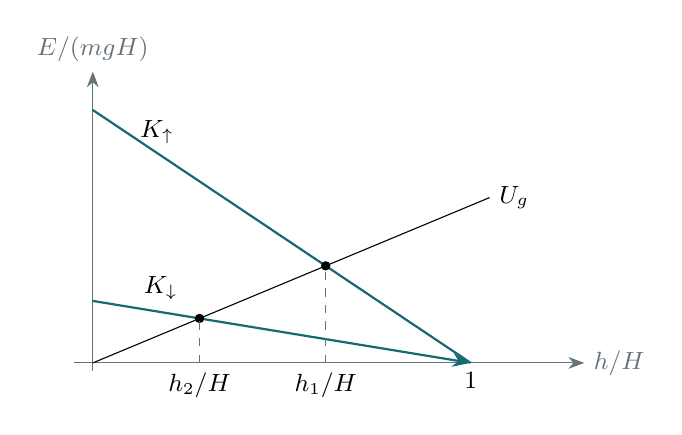
\begin{tikzpicture}[x=4.8cm,y=2cm]
\draw[axis] (-.05,0)--(1.3,0) node[right] {$h/H$};
\draw[axis] (0,-.05)--(0,1.85) node[above] {$E/(mgH)$};
\draw[traj,domain=0:1] plot(\x,{1.606218*(1-\x)});
\draw[motion,domain=0:1] plot(\x,{.393782*(1-\x)});
\draw[thin,domain=0:1.05] plot(\x,\x);
\node[above] at (.17,1.33) {$K_{\uparrow}$};
\node[above] at (.18,.34) {$K_{\downarrow}$};
\node[right] at (1.05,1.05) {$U_g$};
\fill (.616303,.616303) circle(1.7pt);\fill (.282528,.282528) circle(1.7pt);
\draw[guide] (.616303,0)--(.616303,.616303);
\draw[guide] (.282528,0)--(.282528,.282528);
\node[below] at (.616303,0) {$h_1/H$};\node[below] at (.282528,0) {$h_2/H$};
\node[below] at (1,0) {$1$};
\end{tikzpicture}
\figcaption{解图3.3B\quad 取$q=0.35\sqrt3$；两动能曲线在最高点归零，在不同位置与$U_g$相交。}
\end{minipage}\end{center}
两段都经过同一高度$h$时，两次动能相差
$K_{\uparrow}-K_{\downarrow}=2\mu mg(H-h)\cot\theta$。
这正是往返最高点所增加的两段路程的摩擦耗能；
当$\mu\to0$时差值消失，两次相等出现在同一高度$H/2$，但发生在不同的时刻。


\Needspace{5\baselineskip}

\pdfbookmark[3]{关键洞察}{q3-h5}

\subsection*{关键洞察}

一次上滑与一次下滑使用同一个势能函数，却使用不同的动能函数。只要最高点能开始下滑，就要把下滑支也与 $U_g$ 相交。在两次都经过的高度 $h$，下滑支比上滑支少 $2qmg(H-h)$ 的动能，这正是从 $h$ 到 $H$ 往返一段的额外耗能。

\Needspace{5\baselineskip}

\pdfbookmark[3]{易错点}{q3-h6}

\subsection*{易错点}

\begin{itemize}
\item 上滑段从 $O$ 开始计摩擦路程，下滑段从 $H$ 开始，两段初态不同。
\item 最高点能下滑的条件是 $\mu<\tan\theta$，由静摩擦决定。
\item 重力势能始终按 $U_g=mgh$ 计算，零点在 $O$。
\item 先用 $q$ 写出公式，再代入 $\mu=0.35,\theta=30^\circ,g=10\,\mathrm{m/s^2}$。
\end{itemize}

\Needspace{5\baselineskip}

\pdfbookmark[3]{课堂讲解建议}{q3-h7}

\subsection*{课堂讲解建议}

让学生在解图3.3B 上选同一横坐标，比较两支动能的纵坐标，再沿斜面指出多走的两段路程。由这两段的摩擦耗能读出动能差 $2\mu mg(H-h)\cot\theta$。随后写 $K_0=K+U_g+E_{\rm diss}$，问“当 $K=U_g$ 时，初能量还有哪一部分？”学生应指出已耗散的能量。最后把势能零点平移，比较新的势能线与两条动能线的交点。

\Needspace{5\baselineskip}

\pdfbookmark[3]{变式训练}{q3-h8}

\subsection*{变式训练}

\begin{enumerate}
\item 将静、动摩擦系数同时增大到 $\mu\geq\tan\theta$，求相等位置的个数。上滑时，重力和滑动摩擦都沿坡向下，仍有 $H=K_0/[mg(1+q)]$ 和 $h_1=K_0/[mg(2+q)]$。变图3.3V1 取 $q=6/5$，两线在 $h_1/H=(1+q)/(2+q)=11/16$ 处相交。到 $H$ 速度为零，$mg\sin\theta\leq\mu mg\cos\theta$，静摩擦可以平衡沿坡重力。物体停留在 $H$，因此只有上滑途中这个相等位置。
\begin{center}\begin{minipage}{.98\linewidth}\centering
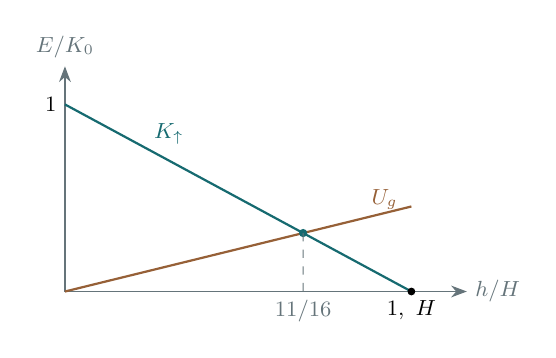
\begin{tikzpicture}[scale=.88,transform shape]
\draw[axis] (0,0)--(5.8,0) node[right] {$h/H$};
\draw[axis] (0,0)--(0,3.25) node[above] {$E/K_0$};
\draw[traj] (0,2.7)--(5,0);
\draw[thick,color=warm] (0,0)--(5,{2.7*5/11});
\coordinate (P) at ({5*11/16},{2.7*5/16});
\fill[accent] (P) circle(1.7pt);
\draw[guide] (P)--({5*11/16},0) node[below] {$11/16$};
\node[above,text=accent] at (1.5,2.0) {$K_{\uparrow}$};
\node[above right,text=warm] at (4.3,1.06) {$U_g$};
\fill (5,0) circle(1.6pt) node[below] {$1,\ H$};
\node[left] at (0,2.7) {$1$};
\end{tikzpicture}
\figcaption{变图3.3V1\quad 取 $q=6/5$。上滑支与重力势能线有一个交点，到最高点后静摩擦维持停留。}
\end{minipage}\end{center}
\item 求返回初始高度时的速率。取 $q<1$，物体从 $H$ 下滑到 $O$，释放重力势能 $mgH$，摩擦耗能 $q\,mgH$，所以 $mv_{\rm return}^2/2=mg(1-q)H$。代入最高点的高度，得到
\[
v_{\rm return}=v_0\sqrt{\frac{1-q}{1+q}}.
\]
完整往返的摩擦耗能为 $2q\,mgH=[2q/(1+q)]K_0$。变图3.3V2 取 $q=1/2$，返回动能为 $K_0/3$、耗能为 $2K_0/3$，故返回速率为 $v_0/\sqrt3$。两次经过 $O$ 的重力势能均为零。
\begin{center}\begin{minipage}{.98\linewidth}\centering
\begin{tikzpicture}[scale=.88,transform shape]
\draw[axis] (0,0)--(5.8,0);
\draw[axis] (0,0)--(0,3.25) node[above] {$E/K_0$};
\filldraw[draw=accent,fill=accent!16] (.75,0) rectangle (1.95,2.7);
\filldraw[draw=accent,fill=accent!16] (3.65,0) rectangle (4.85,.9);
\filldraw[draw=warm,fill=warm!16] (3.65,.9) rectangle (4.85,2.7);
\node at (1.35,1.35) {$1$};
\node at (4.25,.45) {$1/3$};
\node at (4.25,1.8) {$2/3$};
\node[above] at (1.35,2.72) {初始动能};
\node[above] at (4.25,2.72) {返回 $O$};
\node[right,text=accent] at (5,.45) {$K$};
\node[right,text=warm] at (5,1.8) {摩擦耗能};
\node[left] at (0,2.7) {$1$};
\end{tikzpicture}
\figcaption{变图3.3V2\quad 取 $q=1/2$，返回时势能回到零，初动能的三分之二已被摩擦耗散。}
\end{minipage}\end{center}
\item 将初始点的重力势能改记为 $U_0$，求两次相等的位置。势能函数成为 $U_g=U_0+mgh$，而动能随高度的变化仍由各段重力功和摩擦功决定。上滑由 $K_0-mg(1+q)h=U_0+mgh$ 得
\[
h_\uparrow=\frac{K_0-U_0}{mg(2+q)}.
\]
若 $q<1$，下滑由 $mg(1-q)(H-h)=U_0+mgh$ 得
\[
h_\downarrow=\frac{mg(1-q)H-U_0}{mg(2-q)}.
\]
变图3.3V3 取 $q=1/2$、$U_0=K_0/4=3mgH/8$，两次相等发生在 $h_\uparrow=9H/20$、$h_\downarrow=H/12$。在图示的 $0\leq h\leq H$ 内，上滑根存在的条件为 $-mgH\leq U_0\leq K_0$，下滑根存在的条件为 $-mgH\leq U_0\leq mg(1-q)H$。当 $U_0=-mgH$ 时，两根都在 $H$，两段共用同一个到达最高点的时刻。若斜面还向初始点下方延伸，按实际坡长判断下滑根能否到达。
\begin{center}\begin{minipage}{.98\linewidth}\centering
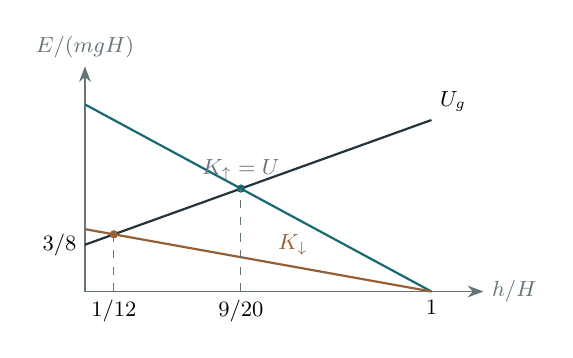
\begin{tikzpicture}[scale=.88,transform shape]
\draw[axis] (0,0)--(5.75,0) node[right] {$h/H$};
\draw[axis] (0,0)--(0,3.25) node[above] {$E/(mgH)$};
\draw[traj] (0,2.7)--(5,0);
\draw[thick,color=warm] (0,.9)--(5,0);
\draw[object] (0,.675)--(5,2.475);
\fill[accent] (2.25,1.485) circle(1.7pt);
\fill[warm] ({5/12},.825) circle(1.7pt);
\draw[guide] (2.25,0)--(2.25,1.485) node[above] {$K_\uparrow=U$};
\draw[guide] ({5/12},0)--({5/12},.825);
\node[below] at (2.25,0) {$9/20$};
\node[below] at ({5/12},0) {$1/12$};
\node[left] at (0,.675) {$3/8$};
\node[above right] at (5,2.475) {$U_g$};
\node[above,text=warm] at (3,.4) {$K_\downarrow$};
\node[below] at (5,0) {$1$};
\end{tikzpicture}
\figcaption{变图3.3V3\quad 取 $q=1/2$、$U_0=K_0/4$，动能曲线保持原状，势能直线上移。}
\end{minipage}\end{center}
\end{enumerate}

\clearpage

\pdfbookmark[2]{第 4 题 桌孔下落绳的速度与位置}{q4}

\section*{第 4 题\quad 桌孔下落绳的速度与位置}

\tagline{M-03-04}

均匀柔软、不可伸长的绳全长为 $l$，一部分平放在光滑水平桌面上，另一部分经过光滑小孔竖直下垂。初始下垂长度 $0<x_0<l$，整绳从静止下落。设桌上绳已经理顺，各段速率相同，小孔只改变运动方向。求绳速 $v(x)$ 及下端位置 $x(t)$，并说明适用时间。

\begin{center}\begin{minipage}{\linewidth}\centering\begin{tikzpicture}
\draw[object] (-2,1.6)--(-.12,1.6);\draw[object] (.12,1.6)--(1.7,1.6);\draw[traj] (-1.8,1.6)--(0,1.6)--(0,-.8);\node[above right] at (.15,1.6) {$O$};\draw[<->] (.7,-.8)--(.7,1.6) node[midway,right] {$x$};
\end{tikzpicture}
\figcaption{图 3.4\quad 向下量取下垂长度。}
\end{minipage}\end{center}

\Needspace{5\baselineskip}

\pdfbookmark[3]{题型定位}{q4-h0}

\subsection*{题型定位}

整根柔绳由桌面经孔口下落的能量题。下垂长度改变重力势能，全绳共同速率决定动能，再由速度与位置关系求时间。

\Needspace{5\baselineskip}

\pdfbookmark[3]{知识点}{q4-h1}

\subsection*{知识点}

均匀绳的势能积分、全绳动能、光滑约束的功、双曲函数与阶段接续。下垂段的质量随长度增加，选全绳作系统时总质量始终为 $\lambda l$。


\Needspace{5\baselineskip}

\pdfbookmark[3]{物理图像}{q4-h2}

\subsection*{物理图像}

解图3.4A 中，桌上段水平趋近孔口，下垂段竖直向下，速率相同。下垂长度增加时，该段的质量和重心深度同时增大，所以势能按 $-x^2$ 下降。到 $x=l$ 时，最后的桌上绳元通过孔口，整绳接着自由下落。

\Needspace{5\baselineskip}

\pdfbookmark[3]{解题入口}{q4-h3}

\subsection*{解题入口}

以孔口为势能零点，按解图3.4A 量下垂长度 $x$。写出
\[
K=\frac12\lambda l v^2,\qquad
U=\int_0^x-\lambda gy\,\dd y=-\frac12\lambda gx^2.
\]
由初值 $x=x_0,v=0$ 写机械能守恒，再以 $v=\dot x$ 分离变量。积分中取 $x=x_0\cosh u$，两项双曲正弦相约后得到时间。

\Needspace{5\baselineskip}

\pdfbookmark[3]{标准解法}{q4-h4}

\subsection*{标准解法}

解图3.4A 中，绳从桌面经过小孔转向下落。整根绳是同一批物质，各段速率相同，以下把全长 $l$、线密度 $\lambda$ 的绳作为系统。桌上部分与下垂部分都计入动能。
\begin{center}\begin{minipage}{\linewidth}\centering\begin{tikzpicture}
\draw[object] (-2,1.6)--(-.12,1.6);\draw[object] (.12,1.6)--(1.7,1.6);\draw[traj] (-1.8,1.6)--(0,1.6)--(0,-.8);\node[above right] at (.15,1.6) {$O$};\draw[<->] (.7,-.8)--(.7,1.6) node[midway,right] {$x$};\fill (0,.4) circle(2pt);\node[left] at (0,.4) {下垂段重心};\node[align=left] at (4,.7) {$K=\tfrac12\lambda l v^2$\\$U=-\tfrac12\lambda gx^2$};
\end{tikzpicture}
\figcaption{解图 3.4A\quad 下垂部分的重心深度为 $x/2$，动能按全绳质量计算。}
\end{minipage}\end{center}

\subsubsection*{整绳的动能和势能}
线密度记为 $\lambda$。绳不可伸长，且桌上部分已经理顺，各段速率同为 $v$，故整绳动能是
\[
K=\frac12\lambda l v^2.
\]
其中 $\lambda x$ 的下垂段沿竖直方向运动，$\lambda(l-x)$ 的桌上段沿水平方向运动，两部分速率相同，动能相加的质量系数为 $\lambda l$。

以下垂方向为正，从桌面向下取微元坐标 $y$。每个微元的重力势能为 $-g y\,\lambda\dd y$，故
\[
U=\int_0^x-\lambda gy\,\dd y=-\frac12\lambda gx^2.
\]
解图 3.4A 的下垂段重心深度为 $x/2$，用 $U=-(\lambda x)g(x/2)$ 也得到同一式子。桌上部分高度为零，无重力势能。

\subsubsection*{速率随位置的变化}
桌面与小孔光滑，只改变绳的方向，约束力不做功。整绳质量固定，能量守恒给出
\[
\frac12\lambda l v^2-\frac12\lambda gx^2
=-\frac12\lambda gx_0^2.
\]
约去 $\lambda/2$ 后，
\[
\boxed{v(x)=\sqrt{\frac gl(x^2-x_0^2)}}.
\]
取正根，因为这一阶段下垂长度单调增加。$x=x_0$ 时速率为零，符合初始条件；$x$ 越大，下垂重力越大，速率也越大。

\subsubsection*{时间积分与接续}
利用 $v=\dot x$，分离变量：
\[
\int_{x_0}^{x}\frac{\dd\xi}{\sqrt{\xi^2-x_0^2}}
=\sqrt{\frac gl}\,t.
\]
令 $\xi=x_0\cosh u$，积分左端等于 $\operatorname{arcosh}(x/x_0)$，得到
\[
\boxed{x(t)=x_0\cosh\!\left(\sqrt{\frac gl}\,t\right)}.
\]
对位置式求导，得到 $\dot x=x_0\sqrt{g/l}\sinh(\sqrt{g/l}\,t)$、$\ddot x=gx/l$。初始速度为零，初始加速度为 $gx_0/l$，它等于下垂段重力 $\lambda gx_0$ 除以全绳质量 $\lambda l$。

绳全部离桌时 $x=l$，对应
\[
t_*=\sqrt{\frac lg}\operatorname{arcosh}\frac l{x_0},\qquad
v_*=\sqrt{\frac gl(l^2-x_0^2)}.
\]
双曲余弦公式只适用于 $0\leq t\leq t_*$。之后整绳自由下落，下端位置应接为
\[
x=l+v_*(t-t_*)+\frac12g(t-t_*)^2.
\]
位置与速度在接续点连续；加速度也由 $gx/l$ 在 $x=l$ 时达到 $g$。
\subsubsection*{沿绳的切向动力学与积分常数}
将整绳分成小段，对每段沿运动方向写切向方程，可以求出牵动全绳的力。
各段的切向加速度都等于$\dot v$；相邻小段的张力在求和时抵消，
光滑孔口的法向约束力不进入切向方程。
于是质量系数为整绳质量$m=\lambda l$，驱动项为下垂段重力$\lambda gx$，即
\[
\lambda l\,\dot v=\lambda gx.
\]
各小段的投影方向随绳走向而变，这条标量式把它们的切向分量相加。桌上段水平运动，下垂段竖直运动；小孔对经过孔口的绳提供法向作用，使速度矢量转向，同时保持速率连续。
由$\dot v=v\,\dd v/\dd x$，有
\[
v\,\dd v=\frac glx\,\dd x,
\qquad v^2=\frac glx^2+C.
\]
初值$x=x_0,v=0$确定$C=-gx_0^2/l$，再选下落的正根，得到前面的$v(x)$。

时间积分中的代换也可展开。令$\xi=x_0\cosh u$，
则$\dd\xi=x_0\sinh u\,\dd u$且$\sqrt{\xi^2-x_0^2}=x_0\sinh u$，
两者约去后积分等于$u$。不定积分的完整形式为
\[
\operatorname{arcosh}(x/x_0)=\sqrt{g/l}\,t+C_t.
\]
$t=0$时$x=x_0$，左端为零，所以$C_t=0$。
解图3.4A 的 $x$ 从孔口量到绳下端，故全绳各段的速率为 $\dot x$。下垂段一面运动，一面纳入从桌面转来的绳元，所以 $x/2$ 表示每一时刻下垂部分的重心深度。它用于求当时的重力势能，全绳动能则按每段的速率 $\dot x$ 相加。


\Needspace{5\baselineskip}

\pdfbookmark[3]{关键洞察}{q4-h5}

\subsection*{关键洞察}

重力势能由当时下垂部分的质量分布给出，动能由全绳所有绳元给出。两者分别带 $x^2$ 和 $lv^2$，因此速率满足 $v^2=g(x^2-x_0^2)/l$。

\Needspace{5\baselineskip}

\pdfbookmark[3]{易错点}{q4-h6}

\subsection*{易错点}

\begin{itemize}
\item 桌上段虽然高度不变，仍以速率 $v$ 运动，计入整绳动能。
\item 下垂段质量为 $\lambda x$，重心深度为 $x/2$，势能为 $-\lambda gx^2/2$。
\item 时间积分的分母为 $\sqrt{x^2-x_0^2}$，对应双曲余弦。
\item 在 $x=l$ 接续自由落体时，保留离桌速度 $v_*$。
\end{itemize}

\Needspace{5\baselineskip}

\pdfbookmark[3]{课堂讲解建议}{q4-h7}

\subsection*{课堂讲解建议}

先沿解图3.4A 分别指向桌上段和下垂段，请学生写出两部分动能，相加得到 $\lambda lv^2/2$。再把下垂长度画成两倍，问其重力势能绝对值怎样变，质量和重心深度都加倍，所以变为四倍。随后把各段切向方程相加，说明质量系数为何仍是 $\lambda l$。最后在 $x=l$ 标出速度箭头，以它作为自由落体的初速度。

\Needspace{5\baselineskip}

\pdfbookmark[3]{变式训练}{q4-h8}

\subsection*{变式训练}

\begin{enumerate}
\item 桌面与绳的静、动摩擦系数均为 $\mu$，求自行启动条件和速率。初始下垂段重量为 $\lambda gx_0$，桌面最大静摩擦为 $\mu\lambda g(l-x_0)$，所以自行启动要求
\[
x_0>x_c=\frac{\mu l}{1+\mu}.
\]
等号时静摩擦可维持静止。移动到 $x$ 时，桌上绳长为 $l-x$，将滑动摩擦随位移积分，耗能为
\[
E_f=\int_{x_0}^x\mu\lambda g(l-\xi)\,\dd\xi
=\mu\lambda g\left[l(x-x_0)-\frac{x^2-x_0^2}{2}\right].
\]
由 $\lambda lv^2/2=\lambda g(x^2-x_0^2)/2-E_f$，得
\[
v^2=\frac gl\left[(1+\mu)(x^2-x_0^2)-2\mu l(x-x_0)\right].
\]
变图3.4V1 中的驱动余量是 $D=\lambda g[(1+\mu)x-\mu l]$。当 $x_0>x_c$，从初态起这条线始终为正并持续上升，绳速随下垂长度增加。若题设只给动摩擦系数，启动条件还需由另给的静摩擦系数确定。
\begin{center}\begin{minipage}{.98\linewidth}\centering
\begin{tikzpicture}[scale=.88,transform shape]
\draw[axis] (0,0)--(6.2,0) node[right] {$u=x/l$};
\draw[axis] (0,-1.45)--(0,2.95) node[above] {$D/(\lambda gl)$};
\draw[thin] (0,-1.2)--(5.5,2.4);
\draw[traj,line width=1.4pt] (2.75,.6)--(5.5,2.4);
\draw[guide] ({5.5/3},0)--({5.5/3},-1.0);
\node[below] at ({5.5/3},-1.0) {$1/3$};
\fill[accent] (2.75,.6) circle(1.7pt);
\draw[guide] (2.75,.6)--(2.75,0) node[below] {$1/2$};
\node[above right] at (2.75,.6) {初态};
\node[below] at (5.5,0) {$1$};
\node[left] at (0,2.4) {$1$};
\end{tikzpicture}
\figcaption{变图3.4V1\quad 取 $\mu=1/2$、$x_0/l=1/2$，启动后驱动余量沿加粗线持续增加。}
\end{minipage}\end{center}
\item 光滑桌面上，求整绳离桌的时间和速度。用 $x=x_0\cosh(t\sqrt{g/l})$ 令 $x=l$，得
\[
t_*=\sqrt{\frac lg}\operatorname{arcosh}\frac l{x_0},\qquad
v_*=\sqrt{\frac gl(l^2-x_0^2)}.
\]
变图3.4V2 取 $x_0=l/2$，离桌的无量纲时刻为 $\operatorname{arcosh}2$，速率为 $\sqrt{3gl}/2$。图中离桌点的两条曲线共用一条切线。之后以 $v_*$ 为初速度，有 $x=l+v_*(t-t_*)+g(t-t_*)^2/2$，加速度也从 $gx/l$ 连续达到 $g$。
\begin{center}\begin{minipage}{.98\linewidth}\centering
\begin{tikzpicture}[scale=.88,transform shape]
\pgfmathsetmacro{\st}{ln(2+sqrt(3))}
\draw[axis] (0,0)--(5.92,0) node[right] {$s=t\sqrt{g/l}$};
\draw[axis] (0,0)--(0,4.05) node[above] {$x/l$};
\draw[traj,domain=0:\st,samples=80] plot ({2.6*\x},{cosh(\x)});
\draw[thick,dashed,color=warm,domain=\st:2.05,samples=70] plot ({2.6*\x},{2*(1+sqrt(3)/2*(\x-\st)+.5*(\x-\st)^2)});
\coordinate (P) at ({2.6*\st},2);
\draw[guide] (0,2)--(P)--({2.6*\st},0);
\fill[accent] (P) circle(1.7pt);
\node[above left] at (P) {离桌};
\node[below] at ({2.6*\st},0) {$\operatorname{arcosh}2$};
\node[left] at (0,1) {$1/2$};\node[left] at (0,2) {$1$};
\node[above right,text=warm] at (4.5,2.85) {自由落体};
\end{tikzpicture}
\figcaption{变图3.4V2\quad 从半长下垂释放，离桌前后的位移线在接续点共用一条切线。}
\end{minipage}\end{center}
\item 初始下垂长度仍为 $x_0$，另给向下初速度 $v_i\geq0$，求位置及离桌时间。沿绳的切向方程为 $\ddot x=gx/l$。取 $\omega=\sqrt{g/l}$，满足 $x(0)=x_0,\dot x(0)=v_i$ 的解为
\[
x(t)=x_0\cosh\omega t+\frac{v_i}{\omega}\sinh\omega t.
\]
变图3.4V3 取 $x_0=l/4$、$v_i=\sqrt{gl}/4$，两项恰好合为 $x/l=e^{\omega t}/4$，因此在 $\omega t=\ln4$ 离桌；从同一位置静止释放则在 $\operatorname{arcosh}4$ 离桌。一般情况下记 $\nu=v_i/\omega$，以 $z=e^{\omega t}$ 改写 $x=l$，得 $(x_0+\nu)z^2-2lz+(x_0-\nu)=0$。取对应未来离桌时刻的根，得到
\[
t_*=\frac1\omega\ln\frac{l+\sqrt{l^2-x_0^2+\nu^2}}{x_0+\nu},
\qquad v_*=\sqrt{v_i^2+\frac gl(l^2-x_0^2)}.
\]
位置公式用到这个时刻为止，随后以此处的位置和速度接续自由落体。
\begin{center}\begin{minipage}{.98\linewidth}\centering
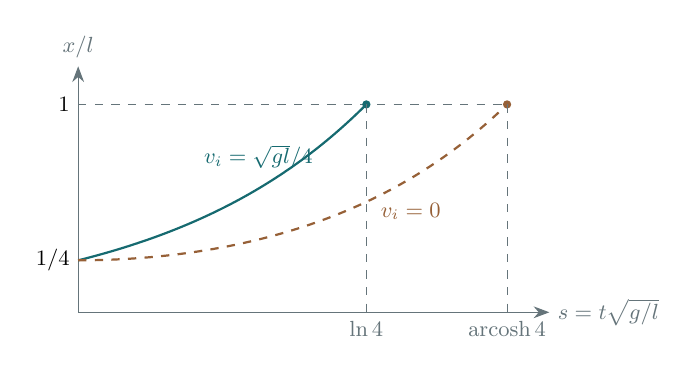
\begin{tikzpicture}[scale=.88,transform shape]
\draw[axis] (0,0)--(6.8,0) node[right] {$s=t\sqrt{g/l}$};
\draw[axis] (0,0)--(0,3.55) node[above] {$x/l$};
\draw[traj,domain=0:1.38629436,samples=80] plot ({3*\x},{.75*exp(\x)});
\draw[thick,dashed,color=warm,domain=0:2.06343707,samples=90] plot ({3*\x},{.75*cosh(\x)});
\draw[guide] (0,3)--(6.19,3);
\fill[accent] ({3*ln(4)},3) circle(1.7pt);
\fill[warm] ({3*ln(4+sqrt(15))},3) circle(1.7pt);
\draw[guide] ({3*ln(4)},3)--({3*ln(4)},0) node[below] {$\ln4$};
\draw[guide] ({3*ln(4+sqrt(15))},3)--({3*ln(4+sqrt(15))},0) node[below] {$\operatorname{arcosh}4$};
\node[left] at (0,.75) {$1/4$};
\node[left] at (0,3) {$1$};
\node[above,text=accent] at (2.6,1.94) {$v_i=\sqrt{gl}/4$};
\node[below,text=warm] at (4.8,1.7) {$v_i=0$};
\end{tikzpicture}
\figcaption{变图3.4V3\quad 相同下垂长度释放，有向下初速度时更早到达 $x=l$；两线均止于离桌点。}
\end{minipage}\end{center}
\end{enumerate}

\clearpage

\pdfbookmark[2]{第 5 题 单摆碰钉后的完整圆周与撞钉条件}{q5}

\section*{第 5 题\quad 单摆碰钉后的完整圆周与撞钉条件}

\tagline{M-03-05}

摆长为 $L$ 的单摆，从悬点 $O$ 左侧、与向下竖直方向夹角 $\alpha$ 处静止释放。右侧钉子 $P$ 满足 $OP=r<L$，$OP$ 与向下竖直方向夹角为 $\beta$，其中 $0<\beta<\alpha\leq90^\circ$。绳转到 $OP$ 方向后绕钉运动，绳与钉均理想光滑。求：\begin{enumerate}\item 完成绕钉圆周运动的最小释放角；\item 绳松弛后，小球沿抛物线直接击中钉子 $P$ 所需的释放角。若条件不能实现，应说明。\end{enumerate}

\begin{center}\begin{minipage}{\linewidth}\centering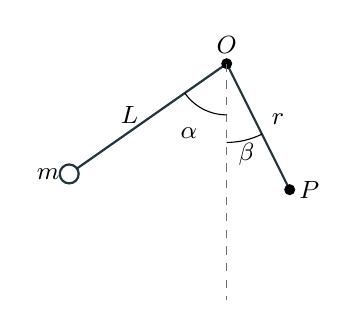
\begin{tikzpicture}
\coordinate(O)at(0,3);\coordinate(P)at(.8,1.4);\coordinate(A)at(-2,1.6);\draw[object] (A)--(O)--(.8,1.4);\fill(O)circle(2pt);\fill(P)circle(2pt);\filldraw[object,fill=white](A)circle(.12);\draw[guide](O)--(0,0);\node[above]at(O){$O$};\node[right]at(P){$P$};\node[left]at(A){$m$};\node[left]at(-1,2.35){$L$};\node[right]at(.45,2.3){$r$};\draw (0,2.35) arc(-90:-145:.65);\node at(-.48,2.12){$\alpha$};\draw (0,2) arc(-90:-63.435:1);\node at(.25,1.85){$\beta$};
\end{tikzpicture}
\figcaption{图 3.5\quad 绳碰钉后，运动半径变为 $a=L-r$。}
\end{minipage}\end{center}

\Needspace{5\baselineskip}

\pdfbookmark[3]{题型定位}{q5-h0}

\subsection*{题型定位}

单摆绕钉后的能量与绳张力。完整圆周由最高点的张力条件确定，撞钉由松绳条件和抛物线命中条件共同确定。

\Needspace{5\baselineskip}

\pdfbookmark[3]{知识点}{q5-h1}

\subsection*{知识点}

碰钉前后以同一个高度零点使用机械能。绕钉半径为 $a=L-r$，能量给速率、径向方程给张力。若张力在到达最高点前降到零，球从当时的切线速度进入抛体运动。求撞钉时，用飞行中球到钉子的距离判断绳是否持续松弛。


\Needspace{5\baselineskip}

\pdfbookmark[3]{物理图像}{q5-h2}

\subsection*{物理图像}

图3.5A 中，绕钉完整一周的最高点在 $P$ 上方，临界速度仍为 $\sqrt{ga}$。图3.5B 中，球在 $D$ 处松绳，此时 $\pi/2<\theta_0<\pi$，切线向左上方，随后抛物线经过 $P$。飞行中的距离 $d_P$ 在 $a$ 内，绳保持松弛。

\Needspace{5\baselineskip}

\pdfbookmark[3]{解题入口}{q5-h3}

\subsection*{解题入口}

由高度写 $v^2=2g(r\cos\beta+a\cos\theta-L\cos\alpha)$，代入径向式求 $T(\theta)$。第一问在 $\theta=\pi$ 令张力达到临界。第二问在未知 $\theta_0$ 令 $T=0$，写松绳位置和速度两分量，由水平命中式求正时间后代入竖直式。

\Needspace{5\baselineskip}

\pdfbookmark[3]{标准解法}{q5-h4}

\subsection*{标准解法}

令 $a=L-r$，以钉子为圆心，$\theta$ 从向下竖直方向量起，如解图 3.5A。球的高度为 $-r\cos\beta-a\cos\theta$（相对 $O$）。
\begin{center}\begin{minipage}{\linewidth}\centering\begin{tikzpicture}
\coordinate(P)at(0,0);\draw[guide](P)circle(1.5);\draw[guide](P)--(0,-1.8);\draw[object](P)--(1.15, .96);\fill(P)circle(2pt);\filldraw[object,fill=white](1.15,.96)circle(.1);\draw[motion](1.15,.96)--(.55,1.68)node[above]{$v$};\draw[force](1.15,.96)--(1.15,.2)node[right]{$mg$};
\draw[force](1.15,.96)--(.575,.48)node[below left]{$T$};\node[left]at(P){$P$};\node[right]at(.65,.4){$a$};\draw (0,-.55) arc(-90:40:.55);\node at(.7,-.3){$\theta$};\node[align=left]at(4,0){$T=mv^2/a+mg\cos\theta$\\松绳处：$T=0$};
\end{tikzpicture}
\figcaption{解图 3.5A\quad 完整圆周的临界状态在最高点确定；撞钉轨道由松绳点接续抛体运动。}
\end{minipage}\end{center}

\subsubsection*{碰钉后的能量与张力}
球绕钉后的半径为 $a=L-r$。相对悬点 $O$，释放点高度为 $-L\cos\alpha$；绕钉位置的高度为 $-r\cos\beta-a\cos\theta$，如解图 3.5A。理想光滑钉不耗能，故
\[
\frac12mv^2=mg(r\cos\beta+a\cos\theta-L\cos\alpha).
\]
取指向 $P$ 为径向正向，张力与重力分量满足
\[
T-mg\cos\theta=\frac{mv^2}{a}.
\]
因此
\[
v^2=2g(r\cos\beta+a\cos\theta-L\cos\alpha),
\]
\[
T=3mg\cos\theta+\frac{2mg}{a}(r\cos\beta-L\cos\alpha).
\]
圆周上的每个位置都需有实速率 $v^2\geq0$；绳力沿半径向内，张紧状态还需 $T\geq0$。在 $\pi/2<\theta<\pi$ 的上行段，$\mathrm dT/\mathrm d\theta=-3mg\sin\theta<0$。若这一段上 $T$ 降到零，沿圆弧继续上行将要求绳沿半径向外推，小球便从该点沿切线进入自由飞行。完整圆周的临界情形在最高点取到张力的零最小值，过最高点后张力重新增大。

\subsubsection*{完整圆周的临界释放角}
在绕钉的上行段，$\cos\theta$ 逐渐减小，张力最低的位置是最高点 $\theta=\pi$。临界时 $T_{\mathrm{top}}=0$。最高点的重力全部用于圆周向心加速度，故 $v_{\mathrm{top}}^2=ga$，速度水平，方向沿圆的切线。
代入张力式，
\[
-3mg+\frac{2mg}{a}(r\cos\beta-L\cos\alpha)=0.
\]
记
\[
C_1=\frac rL\cos\beta-\frac{3a}{2L},
\]
则完整圆周要求 $\cos\alpha\leq C_1$。在 $0<\alpha\leq90^\circ$ 内，余弦随释放角增大而减小，所以
\[
\boxed{\alpha_{\min}=\arccos C_1}.
\]
题设 $\beta<\alpha\leq90^\circ$，即 $0\leq\cos\alpha<\cos\beta$。因此可实现条件是 $C_1\geq0$；当它等于零时，恰从水平位置 $\alpha=90^\circ$ 释放。又因 $C_1<\cos\beta$，可实现时自动有 $\alpha_{\min}>\beta$。

\subsubsection*{松绳后直接击中钉子}
\begin{center}\begin{minipage}{\linewidth}\centering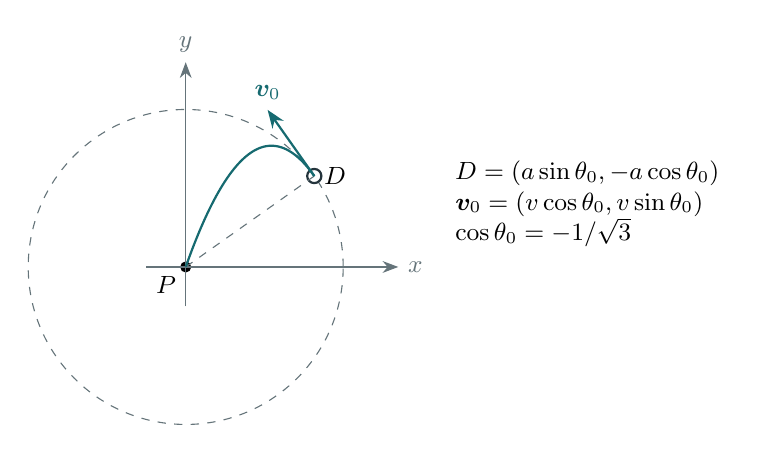
\begin{tikzpicture}
\draw[guide](0,0)circle(2);
\coordinate(P)at(0,0);\coordinate(D)at(1.633,1.155);
\fill(P)circle(2pt);\filldraw[object,fill=white](D)circle(.09);
\draw[guide](P)--(D);\draw[axis](-.5,0)--(2.7,0)node[right]{$x$};
\draw[axis](0,-.5)--(0,2.6)node[above]{$y$};
\draw[traj,domain=0:1,samples=60]plot({1.633*(1-\x)},{1.155+2.309*\x-3.464*\x^2});
\draw[motion](D)--(1.04,1.995)node[above]{$\vect v_0$};
\node[below left]at(P){$P$};\node[right]at(D){$D$};
\node[align=left]at(5.1,.8){$D=(a\sin\theta_0,-a\cos\theta_0)$\\
$\vect v_0=(v\cos\theta_0,v\sin\theta_0)$\\$\cos\theta_0=-1/\sqrt3$};
\end{tikzpicture}
\figcaption{解图 3.5B\quad 松绳后的抛物线直接经过钉子；虚圆是此前的圆周轨道。}
\end{minipage}\end{center}
如解图 3.5B，设松绳点的角度为 $\theta_0\in(\pi/2,\pi)$。由 $T=0$，
\[
v^2=-ag\cos\theta_0.
\]
以 $P$ 为原点，水平向右、竖直向上，松绳位置和速度为
\[
(x_0,y_0)=(a\sin\theta_0,-a\cos\theta_0),\quad
(v_x,v_y)=(v\cos\theta_0,v\sin\theta_0).
\]
飞行时间记为 $\tau$。命中原点要求
\[
0=a\sin\theta_0+v\cos\theta_0\,\tau,\qquad
0=-a\cos\theta_0+v\sin\theta_0\,\tau-\frac12g\tau^2.
\]
第一式给出 $\tau=-a\sin\theta_0/(v\cos\theta_0)>0$。代入第二式并利用 $\sin^2\theta_0+\cos^2\theta_0=1$，得
\[
v^2=-\frac{ag\sin^2\theta_0}{2\cos\theta_0}.
\]
与松绳条件联立，得到 $2\cos^2\theta_0=\sin^2\theta_0$。根据所在象限取
\[
\cos\theta_0=-\frac1{\sqrt3},\qquad
\theta_0\approx125.26^\circ.
\]
再由张力式求释放角：
\[
\boxed{\alpha=\arccos\!\left(\frac rL\cos\beta-
\frac{\sqrt3a}{2L}\right)}.
\]
括号内须非负，才能使 $\alpha\leq90^\circ$；它也小于 $\cos\beta$，故 $\alpha>\beta$ 自动成立。这一释放角确定球在 $\theta_0$ 第一次松绳，速度方向由图3.5B 的圆弧切线给出，之后的抛物线通过 $P$。
\subsubsection*{松绳后的抛体是否会被绳再次拉住}
命中条件还要与绳长相容。以解图3.5B中的$D$为起点，
记从$D$飞到$P$的时间为$\tau_P$。
水平命中式与$\cos\theta_0=-1/\sqrt3$给出
\[
\tau_P=\frac{\sqrt2a}{v},\qquad
v^2=\frac{ag}{\sqrt3},\qquad
\tau_P^2=\frac{2\sqrt3a}{g}.
\]
令$u=\tau/\tau_P$，把速度、时间代入抛体坐标，得到
\[
\frac xa=\sqrt{\frac23}(1-u),\qquad
\frac ya=\frac{1+2u-3u^2}{\sqrt3},\qquad 0\leq u\leq1.
\]
图3.5B 中 $D$ 是固定的松绳点。飞行中的小球到钉子的距离记为 $d_P(\tau)$，满足
\[
\frac{d_P^2(\tau)}{a^2}
=\frac23(1-u)^2+\frac13(1+2u-3u^2)^2
=1-4u^3+3u^4\leq1.
\]
在$0<u<1$内，$u^3(3u-4)<0$，小球始终处在半径$a$的圆内，
绳不会在命中前再次张紧。即使松绳后与钉子的接触方式改变，
由三角不等式，悬点到球的直线距离也不超过$r+d_P<L$，同样不会提前拉紧。
解图3.5B中圆弧之后的实线抛物线因此是可以实际经过的自由飞行段。

碰钉前后的张力随运动位置有如下变化。在碰钉前的长摆段，若位置角为$\psi$，
则$T_O=mg(3\cos\psi-2\cos\alpha)\geq mg\cos\alpha\geq0$。
碰钉后，从$\theta=\beta$到$\theta_0$，
$T(\theta)$随$\cos\theta$减少而下降，第一次到零正是上面求出的松绳点，
不会在到达$D$前就失去圆周约束。
完整圆周的临界条件还给出$v_{\mathrm{top}}^2=ga>0$，
其余位置的高度更低、速率更大，张力也更大，故最高点达到临界时整圈均满足张紧条件。


\Needspace{5\baselineskip}

\pdfbookmark[3]{关键洞察}{q5-h5}

\subsection*{关键洞察}

完整圆周的最高点既要到达，也要有足够向心速率维持绳的张紧。撞钉则在此前松绳，离开圆弧走抛物线。图中两个关键点由各自的动力学与几何条件分别确定。

\Needspace{5\baselineskip}

\pdfbookmark[3]{易错点}{q5-h6}

\subsection*{易错点}

\begin{itemize}
\item 碰钉后的半径为 $L-r$，释放高度仍相对原悬点计算。
\item 最高点张力最低，临界速度满足 $v_{\rm top}^2=ga$。
\item 松绳后从 $D$ 的位置和切线速度写自由飞行，命中方程给 $\cos\theta_0=-1/\sqrt3$，取第二象限。
\item 释放角取 $0\leq\cos\alpha<\cos\beta$ 的范围，飞行中的 $d_P<a$ 使绳在命中前保持松弛。
\end{itemize}

\Needspace{5\baselineskip}

\pdfbookmark[3]{课堂讲解建议}{q5-h7}

\subsection*{课堂讲解建议}

把图3.5A 的最高点与图3.5B 的松绳点分别圈出，先问两个点的向心力如何提供。最高点临界时由重力提供 $mv^2/a$，松绳点则只保留当处重力的径向分量。求完撞钉角后追问“途中绳会不会先拉紧”，请学生用 $d_P^2/a^2=1-4u^3+3u^4$ 指出 $0<u<1$ 时小于1。再将 $\beta=0$，用变图3.5V1 比较两种释放轨道的参数要求。

\Needspace{5\baselineskip}

\pdfbookmark[3]{变式训练}{q5-h8}

\subsection*{变式训练}

\begin{enumerate}
\item 令 $\beta=0$，化简两种释放角与可实现范围。设 $s=r/L$，则 $a/L=1-s$。完整圆周要求 $\cos\alpha\leq C_1=(5s-3)/2$，其临界释放角为 $\arccos C_1$；松绳撞钉要求 $\cos\alpha=C_2=[(2+\sqrt3)s-\sqrt3]/2$。变图3.5V1 中 $C_1=0$ 对应 $s=3/5$，$C_2=0$ 对应 $s=\sqrt3/(2+\sqrt3)$。所以两轨道分别在 $s\geq3/5$ 和 $s\geq\sqrt3/(2+\sqrt3)$ 时能由 $\alpha\leq90^\circ$ 静止释放实现。每条曲线的左端均是 $90^\circ$ 释放。
\begin{center}\begin{minipage}{.98\linewidth}\centering
\begin{tikzpicture}[scale=0.85,transform shape]
\draw[axis] (0,0)--(6.7,0) node[right] {$r/L$};\draw[axis] (0,0)--(0,4.45) node[above] {$\alpha$};
\draw[traj,domain=.6:.98,samples=82] plot ({6*\x},{acos((5*\x-3)/2)/23});
\draw[traj,dashed,domain=.46410162:.98,samples=86] plot ({6*\x},{acos(((2+sqrt(3))*\x-sqrt(3))/2)/23});
\draw[guide] (0,{90/23})--(3.6,{90/23});\node[left] at (0,{90/23}) {$90^\circ$};
\fill (3.6,{90/23}) circle (1.6pt);\fill ({6*sqrt(3)/(2+sqrt(3))},{90/23}) circle (1.6pt);
\node[below] at (3.6,0) {$3/5$};\node[below left] at ({6*sqrt(3)/(2+sqrt(3))},0) {$\sqrt3/(2+\sqrt3)$};
\node[right] at (4.66,3.38) {完整圆周};\node at (4.85,1.76) {撞钉};
\end{tikzpicture}
\figcaption{变图3.5V1\quad $\beta=0$ 时两条释放角曲线分别从 $90^\circ$ 开始。}
\end{minipage}\end{center}
\item 求沿圆轨道到达最高点所需的最小释放角。图3.5V2 中最高点 $Q$ 的径向式是 $T_Q+mg=mv_Q^2/a$。$T_Q\geq0$ 给 $v_Q^2\geq ga$，临界仍是 $v_Q=\sqrt{ga}$，该点是张力随 $\theta$ 变化的最低处。继续沿圆周下行时 $\cos\theta$ 增大，张力回升，因而对应的释放角也是完成整周所需的最小角。若仅按能量令最高点速率为零，则此前的张力会先降到零：把该能量代回径向式，$T=mg(2+3\cos\theta)$，在 $\cos\theta=-2/3$ 已松绳。因而按张紧路径到达 $Q$ 的最低能量保留 $mga/2$ 的动能。
\begin{center}\begin{minipage}{.98\linewidth}\centering
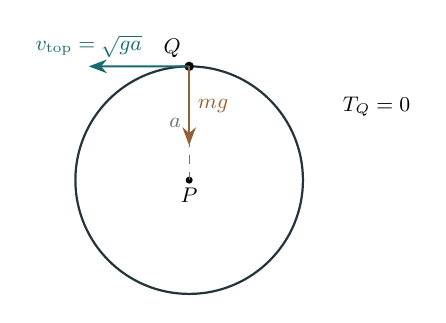
\begin{tikzpicture}[scale=0.85,transform shape]
\draw[object] (0,0) circle (1.7);\fill (0,0) circle (1.5pt) node[below] {$P$};
\coordinate (T) at (0,1.7);\fill (T) circle (2pt) node[above left] {$Q$};
\draw[guide] (0,0)--(T) node[midway,left] {$a$};\draw[motion] (T)--(-1.5,1.7) node[above] {$v_{\rm top}=\sqrt{ga}$};
\draw[force] (T)--(0,.52) node[midway,right] {$mg$};\node at (2.8,1.1) {$T_Q=0$};
\end{tikzpicture}
\figcaption{变图3.5V2\quad 最高点的重力指向圆心，临界情况下独自提供向心加速度。}
\end{minipage}\end{center}
\item 给定 $\beta$，求能由不超过 $90^\circ$ 的释放角完成圆周的最小 $r/L$。由 $C_1=s\cos\beta-3(1-s)/2\geq0$，整理得
\[
\frac rL\geq\frac3{3+2\cos\beta}.
\]
变图3.5V3 在 $\beta=0$ 处为 $3/5$，在 $60^\circ$ 处为 $3/4$，随 $\beta$ 增大逐渐接近1。等号使 $C_1=0$，对应从 $\alpha=90^\circ$ 释放；若希望释放角更小，则须把 $r/L$ 取得更大。
\begin{center}\begin{minipage}{.98\linewidth}\centering
\begin{tikzpicture}[scale=0.85,transform shape]
\draw[axis] (0,0)--(6.4,0) node[right] {$\beta$};\draw[axis] (0,0)--(0,4.2) node[above] {$(r/L)_{\min}$};
\draw[traj,domain=0:85,samples=76] plot ({\x/15},{4*3/(3+2*cos(\x))});
\draw[guide] (4,0)--(4,3)--(0,3);\fill (4,3) circle (1.6pt) node[above left] {$P$};
\node[below] at (4,0) {$60^\circ$};\node[left] at (0,3) {$3/4$};\node[left] at (0,2.4) {$3/5$};
\end{tikzpicture}
\figcaption{变图3.5V3\quad 完整圆周所需的最小钉距比，$P$ 对应 $\beta=60^\circ$。}
\end{minipage}\end{center}
\end{enumerate}

\clearpage

\pdfbookmark[2]{第 6 题 圆环双球下滑与悬线张力}{q6}

\section*{第 6 题\quad 圆环双球下滑与悬线张力}

\tagline{M-03-06}

质量 $M$、半径 $R$ 的竖直圆环，用轻细线悬挂。环上串着两个质量均为 $m$ 的光滑小球，从顶端以无限小扰动同时向两侧滑下。$\theta$ 从向上竖直半径量起。\begin{enumerate}\item 假设圆环不动，画出悬线张力 $T$ 随 $x=\cos\theta$ 的曲线，求最小值及对应角度。\item 求圆环可能上升的质量比阈值，画出阈值情形的曲线，并区分“张力为零”与“实际上升”。\end{enumerate}

\begin{center}\begin{minipage}{\linewidth}\centering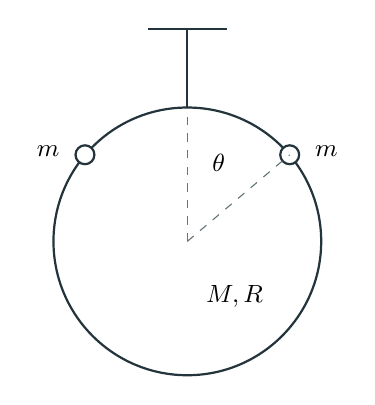
\begin{tikzpicture}
\draw[object](0,0)circle(1.7);\draw[object](0,1.7)--(0,2.7);\draw[object](-.5,2.7)--(.5,2.7);\filldraw[object,fill=white](1.3,1.1)circle(.12);\filldraw[object,fill=white](-1.3,1.1)circle(.12);\draw[guide](0,0)--(0,1.7);\draw[guide](0,0)--(1.3,1.1);\node at(.4,1){$\theta$};\node[right]at(1.5,1.15){$m$};\node[left]at(-1.5,1.15){$m$};\node at(.6,-.7){$M,R$};
\end{tikzpicture}
\figcaption{图 3.6\quad 小球串在环上，可承受环沿径向的推、拉作用。}
\end{minipage}\end{center}

\Needspace{5\baselineskip}

\pdfbookmark[3]{题型定位}{q6-h0}

\subsection*{题型定位}

两对称串珠下滑时，圆环所受的竖直作用力与悬线张力。先按圆环固定求函数，再由悬线只能拉的条件判断保持固定的区间。

\Needspace{5\baselineskip}

\pdfbookmark[3]{知识点}{q6-h1}

\subsection*{知识点}

机械能给单球速度，径向方程给环对球的有符号力。两球水平反作用力相消，竖直分量相加。张力随 $x=\cos\theta$ 是开口向上的二次函数，顶点和零点确定阈值与首次松弛位置。


\Needspace{5\baselineskip}

\pdfbookmark[3]{物理图像}{q6-h2}

\subsection*{物理图像}

图3.6B 中环力沿外径取正。过 $x=2/3$ 后，球受力转向圆心，对环的反作用力转向外侧；两球对环的向上分量可能超过环重。图3.6A 的阈值曲线在 $x=1/3$ 处触到零。小球从顶端下滑时，沿横轴从右向左读。

\Needspace{5\baselineskip}

\pdfbookmark[3]{解题入口}{q6-h3}

\subsection*{解题入口}

写 $v^2=2gR(1-x)$，代入 $N-mgx=-mv^2/R$ 得 $N=mg(3x-2)$。再写环的竖直平衡 $T-Mg-2Nx=0$。配方读最小值，解 $T=0$ 时按 $x$ 从1减小的运动顺序取第一个根。

\Needspace{5\baselineskip}

\pdfbookmark[3]{标准解法}{q6-h4}

\subsection*{标准解法}

小球的速度满足 $v^2=2gR(1-\cos\theta)$。取小球所受环力 $N$ 以沿半径向外为正，径向方程给出 $N=mg(3\cos\theta-2)$。解图 3.6A 的曲线采用阈值质量比。
\begin{center}\begin{minipage}{\linewidth}\centering\begin{tikzpicture}
\draw[axis](-2.2,0)--(2.2,0)node[right]{$x$};\draw[axis](0,-.2)--(0,3.4)node[above]{$T/(Mg)$};\draw[traj,domain=-1:1,samples=80]plot({2*\x},{.18*(3*\x-1)^2});\draw[guide](.6667,0)--(.6667,.6);\node[below]at(.6667,0){$1/3$};\node[below]at(-2,0){$-1$};\node[below]at(2,0){$1$};\node[left]at(0,.18){$1$};\node[align=left]at(5,1.8){阈值 $m/M=3/2$\\$T/(Mg)=(3x-1)^2$\\曲线在 $x=1/3$ 与横轴相切};
\end{tikzpicture}
\figcaption{解图 3.6A\quad 阈值时只触及零张力，没有一段需要负张力的区域。}
\end{minipage}\end{center}

\subsubsection*{先按圆环固定计算反力}
每球从环顶下降的高度为 $R(1-\cos\theta)$，由能量守恒，
\[
v^2=2gR(1-\cos\theta).
\]
小球串在环上，环既能将它向外推，也能向内拉。设环对球的径向作用力 $N$ 以向外为正。向外方向的重力分量为 $-mg\cos\theta$，向外加速度为 $-v^2/R$，故
\[
N-mg\cos\theta=-\frac{mv^2}{R},\qquad
N=mg(3\cos\theta-2).
\]
当 $N<0$，环对串珠的作用力沿半径向内。串珠套在环上，仍沿圆弧运动，图3.6B 中对环的反作用力随之改向。

\begin{center}\begin{minipage}{\linewidth}\centering\begin{tikzpicture}
\draw[guide](0,0)circle(1.65);
\filldraw[object,fill=white](1,1.312)circle(.09);
\draw[guide](0,0)--(1,1.312);\draw[force](1,1.312)--(1.48,1.94)node[right]{$N$};
\draw[force](1,1.312)--(1,.35)node[right]{$mg$};
\node at(0,-2){单球受力};
\draw[object](5,0)circle(1.65);\draw[object](5,1.65)--(5,2.2);
\draw[force](5,2.2)--(5,3.1)node[right]{$T$};
\draw[force](5,0)--(5,-.9)node[right]{$Mg$};
\draw[force](4,1.312)--(4.45,.72)node[left]{$-N$};
\draw[force](6,1.312)--(5.55,.72)node[right]{$-N$};
\node at(5,-2){圆环受力};
\end{tikzpicture}
\figcaption{解图 3.6B\quad 球与环的作用力、反作用力分开画；$N$ 按外径正向取有符号值。}
\end{minipage}\end{center}
解图 3.6B 中，球对环的反作用力为 $-N$ 沿半径，其竖直分量为 $-N\cos\theta$。两球的水平分量相互抵消。圆环不动时，竖直平衡为
\[
T-Mg-2N\cos\theta=0.
\]
令 $x=\cos\theta$，得
\[
\boxed{T(x)=Mg+2mg(3x^2-2x)},\quad -1\leq x\leq1.
\]

\subsubsection*{抛物线的顶点与阈值}
以抛物线的顶点配方：
\[
T(x)=6mg\left(x-\frac13\right)^2+Mg-\frac23mg.
\]
所以
\[
\boxed{T_{\min}=Mg-\frac23mg},\quad
\boxed{\theta_{\min}=\arccos(1/3)\approx70.53^\circ}.
\]
运动时 $x$ 从 $1$ 向 $-1$ 变化，曲线先降后升。若 $m/M<3/2$，最低值仍为正，悬线可始终维持环不动。

当 $m/M=3/2$ 时，解图 3.6A 给出
\[
\boxed{\frac{T}{Mg}=(3x-1)^2}.
\]
曲线只在 $x=1/3$ 与零线相切。在这一瞬间，悬线张力为零。顶点两侧的所需张力均为正，因此曲线在整个运动区间仍能由向上的悬线力实现。阈值质量比对应的是一瞬间的零张力。

\subsubsection*{实际开始上升的位置}
若 $m/M>3/2$，假设固定的计算会出现 $T<0$。此时保持环固定需要向下的力，悬线所能给出的拉力却只能向上，所以圆环转入悬线松弛后的运动。求 $T=0$ 的两根：
\[
x_\pm=\frac{1\pm\sqrt{1-3M/(2m)}}3.
\]
因为小球运动时 $x$ 从 $1$ 下降，先遇到较大根，故
\[
\boxed{\theta_{\mathrm{lift}}=\arccos x_+},\qquad
\boxed{\frac mM>\frac32\text{ 时可实际上升}}.
\]
环开始运动后，球与环之间有能量、动量交换，以上“环固定”的速度和张力函数只用到约束失效的一刻。顶端的静止状态本身为不稳定平衡，本题释放理解为给无限小扰动再取极限。
\subsubsection*{函数取值、判别式与可实现的曲线段}
若用求导法，
\[
\frac{\dd T}{\dd x}=12mgx-4mg=0
\quad\Longrightarrow\quad x=\frac13,
\qquad\frac{\dd^2T}{\dd x^2}=12mg>0.
\]
顶点在实际范围$[-1,1]$内，所以给出的确是整个固定环模型的最小张力。
从环顶、水平侧点到环底，分别代入 $x=1,0,-1$，可读出
\begin{center}
\begin{tabular}{@{}rrrrrr@{}}\toprule
$x=\cos\theta$ & $-1$ & $0$ & $1/3$ & $2/3$ & $1$\\\midrule
$T$ & $Mg+10mg$ & $Mg$ & $Mg-2mg/3$ & $Mg$ & $Mg+2mg$\\
$m/M=3/2$时$T/(Mg)$ & 16 & 1 & 0 & 1 & 4\\\bottomrule
\end{tabular}
\end{center}
从环顶到环底，读表方向是$x=1$到$x=-1$，与横轴数值增加的方向相反。
解图3.6C在同一坐标中比较三种质量比，便于区分最低张力为正、相切与出现负值三种情形。
\begin{center}\begin{minipage}{\linewidth}\centering
\begin{tikzpicture}
\draw[axis] (-2.25,0)--(2.3,0) node[right] {$x$};
\draw[axis] (0,-.32)--(0,3.2) node[above] {$T/(Mg)$};
\foreach \x/\lab in {-2/{-1},.666667/{1/3},2/{1}}{\draw (\x,-.04)--(\x,.04);\node[below] at (\x,-.04) {$\lab$};}
\foreach \y/\lab in {.14/1,1.4/10,2.8/20}{\draw (-.04,\y)--(.04,\y);\node[left] at (-.04,\y) {$\lab$};}
\draw[thin,domain=-1:1,samples=100] plot({2*\x},{.14*(1+2*(3*(\x)^2-2*\x))});
\draw[traj,domain=-1:1,samples=100] plot({2*\x},{.14*(3*\x-1)^2});
\draw[force,dashed,domain=-1:.5,samples=100] plot({2*\x},{.14*(1+4*(3*(\x)^2-2*\x))});
\draw[force,domain=.5:1,samples=50] plot({2*\x},{.14*(1+4*(3*\x^2-2*\x))});
\fill (1,0) circle(1.8pt);\draw[guide] (1,.04)--(1,.7);\node[above] at (1.2,.8) {$x_+=1/2$};
\draw[thin] (3,2.8)--(3.65,2.8) node[right] {$m/M=1$};
\draw[traj] (3,2.25)--(3.65,2.25) node[right] {$m/M=3/2$};
\draw[force] (3,1.7)--(3.65,1.7) node[right] {$m/M=2$};
\node[align=left,anchor=north west] at (3,1.35) {曲线均按环固定求得\\$m/M=2$时仅$x\geq1/2$\\属于实际固定环阶段\\虚线为失效后的形式延拓};
\end{tikzpicture}
\figcaption{解图3.6C\quad 不同质量比下保持圆环固定所需的张力；质量比超过阈值时，实线止于首次松弛点，虚线给出固定环的形式延拓。}
\end{minipage}\end{center}

从圆环受力也能推出相同阈值。悬线松弛时，
小球作用于环的向上合力必须至少抵消$Mg$，故
\[
-2N\cos\theta\geq Mg,
\qquad 3x^2-2x+\frac{M}{2m}\leq0.
\]
这个开口向上的二次式要存在非正值，必须有
\[
\Delta=4-4\cdot3\cdot\frac{M}{2m}
=4-\frac{6M}{m}\geq0,
\qquad\frac mM\geq\frac32.
\]
等号只给一个零点，严格大于才给两个不同零点及其间的负张力需求。
圆环刚离开固定位置时，记环心的向上位移为 $Y$，球相对圆环的切向速率为 $v$。球的向外径向加速度是 $\ddot Yx-v^2/R$，所以环对每球的作用为 $N=m(g+\ddot Y)x-mv^2/R$。与圆环的竖直方程联立，
\[
(M+2mx^2)\ddot Y=T-Mg-2m(gx-v^2/R)x.
\]
在图3.6C 的首次零点，$T=0$，右侧等于零，$\ddot Y=0$。紧接着 $x$ 继续减小，右侧从零开始增大：在离位瞬间 $v$ 的变化率仍与固定环时相同，因而右侧的时间导数等于图中有符号固定环张力的负时间导数。分母 $M+2mx^2>0$，所以环开始向上。曲线虚线段只给出保持圆环固定所需的外力；环抬起时悬线张力取零。


\Needspace{5\baselineskip}

\pdfbookmark[3]{关键洞察}{q6-h5}

\subsection*{关键洞察}

串珠的径向力可以沿两个方向，悬线张力取非负值。函数在零线相切时，只有一个瞬间所需悬线力为零；函数穿过零线时，环固定所需的力在一段区间向下，悬线因而松弛。

\Needspace{5\baselineskip}

\pdfbookmark[3]{易错点}{q6-h6}

\subsection*{易错点}

\begin{itemize}
\item 环对球为 $N\vect e_r$，球对环为 $-N\vect e_r$。竖直投影还要乘 $x$。
\item 极值点 $x=1/3$ 位于 $[-1,1]$，两个端点分别对应环底和环顶。
\item 有两零点时，小球下行先到较大的余弦根 $x_+$。
\item 图3.6C 中首次零点之后的固定环延拓，用来表示所需外力；实际松弛悬线的张力为零。
\end{itemize}

\Needspace{5\baselineskip}

\pdfbookmark[3]{课堂讲解建议}{q6-h7}

\subsection*{课堂讲解建议}

让学生分别在单球和圆环图中画作用力与反作用力，再问“哪一个竖直分量进入悬线张力”，答为球对环的 $-Nx$。依次板书 $v^2,N,T$，并说明每个量属于哪个物体。比较变图3.6V3 的三条曲线，请学生从 $x=1$ 向左指出第一次零点。最后换成可推拉的杆，问负 $T$ 对应什么方向，答为杆向下推环。

\Needspace{5\baselineskip}

\pdfbookmark[3]{变式训练}{q6-h8}

\subsection*{变式训练}

\begin{enumerate}
\item 取 $m=2M$，求第一次悬线松弛时的角。由 $T/(Mg)=12x^2-8x+1=12(x-1/2)(x-1/6)$，两根为 $1/2,1/6$。变图3.6V1 中小球从 $x=1$ 向左移动，先到 $P$，故首次松弛角是 $\theta=\arccos(1/2)=60^\circ$。此后运动应连同圆环的位移重新计算，图中虚线保留固定环假设的外力需求。
\begin{center}\begin{minipage}{.98\linewidth}\centering
\begin{tikzpicture}[scale=0.85,transform shape]
\draw[axis] (0,0)--(6.6,0) node[right] {$x=\cos\theta$};\draw[axis] (0,-.65)--(0,3.9) node[above] {$T/(Mg)$};
\draw[traj,domain=.5:1,samples=65] plot ({6*\x},{.65*(12*\x^2-8*\x+1)});
\draw[traj,dashed,domain=0:.5,samples=65] plot ({6*\x},{.65*(12*\x^2-8*\x+1)});
\fill (3,0) circle (1.6pt) node[above left] {$P$};\fill (1,0) circle (1.6pt) node[below] {$1/6$};\node[below] at (3,0) {$1/2$};
\draw[motion] (5.5,3.55)--(4.3,3.55) node[midway,above] {下行};
\end{tikzpicture}
\figcaption{变图3.6V1\quad $m=2M$ 时，实线止于首次松弛点 $P$，虚线为固定环的延拓。}
\end{minipage}\end{center}
\item 将悬线换成可推拉的轻杆，怎样解释 $T<0$？仍把杆对环向上作用取正，则 $T<0$ 给向下的推力，杆可承担它，环继续固定。变图3.6V2 取 $m=2M,x=1/3$，单球 $N=-mg$。两球对环的向上合力为 $2mg/3=4Mg/3$，超过环重的 $Mg/3$ 由杆向下抵消，故 $T=-Mg/3$。有推力能力的杆使这一固定位置可实现。
\begin{center}\begin{minipage}{.98\linewidth}\centering
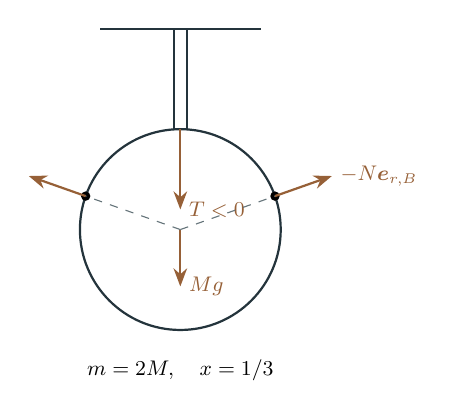
\begin{tikzpicture}[scale=0.85,transform shape]
\draw[object] (0,0) circle (1.5);\draw[object] (-.1,1.5) rectangle (.1,3);\draw[object] (-1.2,3)--(1.2,3);
\coordinate (B) at ({sqrt(2)},{.5});\coordinate (A) at ({-sqrt(2)},{.5});
\fill (A) circle (2pt);\fill (B) circle (2pt);
\draw[force] (0,1.5)--(0,.3) node[right] {$T<0$};
\draw[force] (B)--++(.85,.3) node[right] {$-N\vect e_{r,B}$};
\draw[force] (A)--++(-.85,.3);
\draw[force] (0,0)--(0,-.85) node[right] {$Mg$};
\draw[guide] (0,0)--(A);\draw[guide] (0,0)--(B);\node at (0,-2.1) {$m=2M,\quad x=1/3$};
\end{tikzpicture}
\figcaption{变图3.6V2\quad 换成轻杆后，两个球对环的向上合力由重力和杆的向下推力共同平衡。}
\end{minipage}\end{center}
\item 比较 $m/M=1,3/2,2$ 的曲线。由 $T/(Mg)=1+(m/M)(6x^2-4x)$，三个式子依次为 $6x^2-4x+1$、$9x^2-6x+1$、$12x^2-8x+1$。配方后顶点都在 $x=1/3$，最小值依次为 $1/3,0,-1/3$。变图3.6V3 第一条在零线上方，第二条触零，第三条过零于 $1/2$ 和 $1/6$。按从右向左的下行顺序，第三种情形首先在 $1/2$ 离开固定环过程。
\begin{center}\begin{minipage}{.98\linewidth}\centering
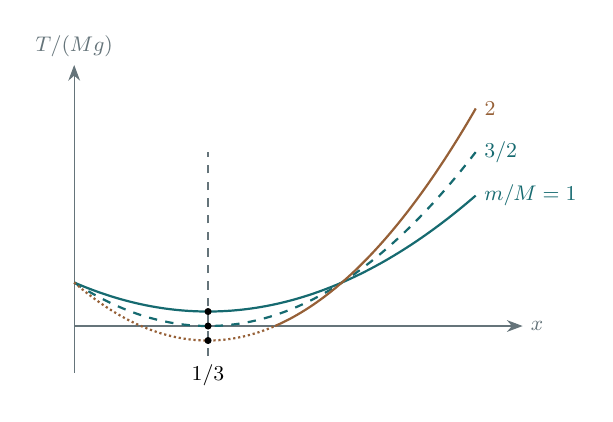
\begin{tikzpicture}[scale=0.85,transform shape]
\draw[axis] (0,0)--(6.7,0) node[right] {$x$};\draw[axis] (0,-.7)--(0,3.9) node[above] {$T/(Mg)$};
\draw[traj,domain=0:1,samples=85] plot ({6*\x},{.65*(6*\x^2-4*\x+1)}) node[right] {$m/M=1$};
\draw[traj,dashed,domain=0:1,samples=85] plot ({6*\x},{.65*(9*\x^2-6*\x+1)}) node[right] {$3/2$};
\draw[warm,thick,densely dotted,domain=0:.5,samples=65] plot ({6*\x},{.65*(12*\x^2-8*\x+1)});
\draw[warm,thick,domain=.5:1,samples=65] plot ({6*\x},{.65*(12*\x^2-8*\x+1)}) node[right] {$2$};
\draw[guide] (2,-.45)--(2,2.6);\node[below] at (2,-.45) {$1/3$};
\fill (2,{.65/3}) circle (1.5pt);\fill (2,0) circle (1.5pt);\fill (2,{-.65/3}) circle (1.5pt);
\end{tikzpicture}
\figcaption{变图3.6V3\quad 三条曲线的顶点横坐标都为 $1/3$。橙色实线在 $x=1/2$ 结束，点线给出假定环继续固定的外力。}
\end{minipage}\end{center}
\item 令 $m/M\to0$，求张力主项并解释环底值。将 $T=Mg+2mg(3x^2-2x)$ 写成 $T=Mg+O(mg)$，故主项为环重。变图3.6V4 取质量比0.02，整个曲线在 $Mg$ 附近。环底 $x=-1$ 时，单球速率满足 $v^2=4gR$，向上径向方程给 $|N|=5mg$，两球对环向下共作用 $10mg$，所以 $T=Mg+10mg$。
\begin{center}\begin{minipage}{.98\linewidth}\centering
\begin{tikzpicture}[scale=0.85,transform shape]
\draw[axis] (0,0)--(6.7,0) node[right] {$x$};\draw[axis] (0,0)--(0,6.75) node[above] {$T/(Mg)$};
\draw[guide] (0,3)--(6.15,3) node[right] {$1$};
\draw[traj,domain=-1:1,samples=85] plot ({3*(\x+1)},{15*(1+.02*(6*(\x)^2-4*\x)-.8)});
\node[left] at (0,0) {$0.8$};\node[left] at (0,3) {$1$};\node[left] at (0,6) {$1.2$};\node[below] at (0,0) {$-1$};\node[below] at (6,0) {$1$};
\fill (0,6) circle (1.5pt) node[right] {$x=-1,\ T/(Mg)=1.2$};
\end{tikzpicture}
\figcaption{变图3.6V4\quad 取 $m/M=0.02$，曲线在 $T=Mg$ 附近，环底的修正为 $10mg$。}
\end{minipage}\end{center}
\end{enumerate}

\clearpage

\pdfbookmark[2]{第 7 题 滑杆脱离约束后的落点}{q7}

\section*{第 7 题\quad 滑杆脱离约束后的落点}

\tagline{M-03-07}

长 $2r=20\,\mathrm{cm}$ 的理想轻杆，在中心 $C$ 固定质量为 $m$ 的质点。端点 $A$ 靠在光滑竖直墙上，端点 $B$ 支在光滑水平地面上。杆从近似竖直的位置由静止下滑，运动始终在同一竖直平面。按集中质量轻杆模型，求中心 $C$ 第一次触地时距墙角 $O$ 的水平距离。

\begin{center}\begin{minipage}{\linewidth}\centering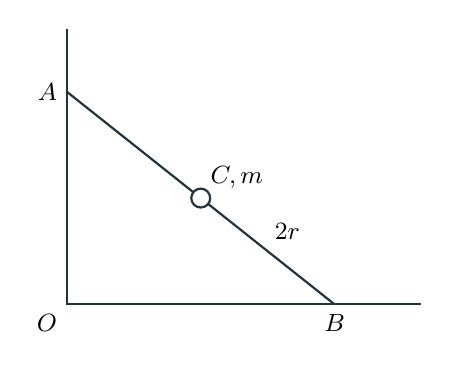
\begin{tikzpicture}
\draw[object](0,3.5)--(0,0)--(4.5,0);\draw[object](0,2.7)--(3.4,0);\filldraw[object,fill=white](1.7,1.35)circle(.12);\node[left]at(0,2.7){$A$};\node[below]at(3.4,0){$B$};\node[above right]at(1.7,1.35){$C,m$};\node[below left]at(0,0){$O$};\node[above]at(2.8,.7){$2r$};
\end{tikzpicture}
\figcaption{图 3.7\quad 两端保持接触时，杆中心沿半径 $r$ 的四分之一圆运动。}
\end{minipage}\end{center}

\Needspace{5\baselineskip}

\pdfbookmark[3]{题型定位}{q7-h0}

\subsection*{题型定位}

滑杆中心的圆弧运动与脱离后的抛体。几何确定中心轨迹，能量确定速率，接触力给阶段转换的位置，脱离的切线速度给出落点。

\Needspace{5\baselineskip}

\pdfbookmark[3]{知识点}{q7-h1}

\subsection*{知识点}

直角三角形斜边中点到三个顶点的距离相等。轻杆零转动惯量使两支持力对中心的力矩相抵；合力沿 $OC$，不做功。单侧支持力在共同零点终止圆弧阶段。


\Needspace{5\baselineskip}

\pdfbookmark[3]{物理图像}{q7-h2}

\subsection*{物理图像}

解图3.7A 中，墙端向下、地面端向右，中心先沿半径 $r$ 的圆弧移动。在 $D$ 处两端反力为零，中心沿右下切线进入抛物线。解图3.7B 的矩形把中心的圆轨迹与两个端点的直线路径联系起来。

\Needspace{5\baselineskip}

\pdfbookmark[3]{解题入口}{q7-h3}

\subsection*{解题入口}

先写 $A,B,C$ 坐标和力矩关系，得到支持力合量沿 $OC$。用 $v^2=2gr(1-\cos\theta)$ 与径向方程求 $N$，令 $N=0$ 得 $\cos\theta_d=2/3$。将脱离位置和速度两分量代入抛体，取落地时间的正根，再加上原有的 $x_d$。

\Needspace{5\baselineskip}

\pdfbookmark[3]{标准解法}{q7-h4}

\subsection*{标准解法}

两端均接触时，$C=(r\sin\theta,r\cos\theta)$，其中 $\theta$ 从竖直方向量起。轻杆对 $C$ 的转动惯量为零，端点支持力的合力沿 $OC$，故中心运动等效于从圆弧外侧滑落。
\begin{center}\begin{minipage}{\linewidth}\centering\begin{tikzpicture}
\draw[axis](0,0)--(4,0)node[right]{$x$};\draw[axis](0,0)--(0,3)node[above]{$y$};\draw[guide](0,2.4)arc(90:0:2.4);\coordinate(D)at(1.789,1.6);\fill(D)circle(2pt);\draw[object](0,0)--(D);\draw[motion](D)--(2.4,.917)node[right]{$v_d$};\draw[traj,domain=0:1,samples=40]plot({1.789+.910*\x},{1.6-1.018*\x-.582*\x^2});\node[above right]at(D){$D$};\node[below]at(2.699,0){落点};\node[align=left]at(5.8,1.8){$\cos\theta_d=2/3$\\先圆周，后抛体};
\end{tikzpicture}
\figcaption{解图 3.7A\quad 离开圆轨迹时，速度沿切线向右下方。}
\end{minipage}\end{center}

\subsubsection*{接触阶段的轨迹与合力方向}
令杆与竖直方向夹角为 $\theta$。两端接触墙、地面时，杆长关系给出
\[
A=(0,2r\cos\theta),\quad B=(2r\sin\theta,0),\quad
C=(r\sin\theta,r\cos\theta).
\]
所以 $OC=r$，中心沿圆弧运动。设墙的水平支持力为 $N_A$，地面的竖直支持力为 $N_B$。轻杆质量忽略不计，对 $C$ 的合力矩必须为零：
\[
N_B\,r\sin\theta=N_A\,r\cos\theta.
\]
因而 $N_A/N_B=\tan\theta$，两支持力合力沿 $OC$ 向外。它始终与中心速度垂直，接触阶段不做功。

取起始倾角趋于零的极限，中心起始高度趋于 $r$。它下降到 $r\cos\theta$ 时，由能量守恒有
\[
v^2=2gr(1-\cos\theta).
\]
向外的径向运动方程为
\[
N-mg\cos\theta=-\frac{mv^2}{r},
\quad N=mg(3\cos\theta-2).
\]
随 $\cos\theta$ 减小，合支持力 $N$ 降低。$N_A=N\sin\theta$、$N_B=N\cos\theta$，所以当 $N=0$，两端支持力同时为零。

\subsubsection*{离位位置和切线速度}
由 $N=0$ 得 $\cos\theta_d=2/3$、$\sin\theta_d=\sqrt5/3$，
\[
x_d=\frac{\sqrt5}{3}r,\quad y_d=\frac23r,\quad
v_d=\sqrt{\frac{2gr}{3}}.
\]
解图 3.7A 中切线向右下方，分量为
\[
v_{dx}=v_d\cos\theta_d=\frac23v_d,\qquad
v_{dy}=-v_d\sin\theta_d=-\frac{\sqrt5}{3}v_d.
\]
集中质量轻杆模型中，两端反力消失后，$C$ 从这一位置和切线速度开始只受重力的抛体运动。

\subsubsection*{取落地时间的正根}
以离位时刻为 $\tau=0$，
\[
x=x_d+v_{dx}\tau,\qquad
y=y_d+v_{dy}\tau-\frac12g\tau^2.
\]
令 $y=0$，得到
\[
\tau=\frac{v_{dy}+\sqrt{v_{dy}^2+2gy_d}}{g}.
\]
根号内 $v_{dy}^2+2gy_d=46gr/27$。代入水平位移并整理：
\[
v_{dx}\tau
=\frac{4r}{27}(\sqrt{23}-\sqrt5),
\]
\[
\boxed{x_{\mathrm{land}}
=\frac{5\sqrt5+4\sqrt{23}}{27}\,r}.
\]
本题 $r=0.10\,\mathrm m$，所以
\[
\boxed{x_{\mathrm{land}}\approx0.11246\,\mathrm m=11.25\,\mathrm{cm}}.
\]
离位时中心已距墙 $7.45\,\mathrm{cm}$；随后水平前进约 $3.79\,\mathrm{cm}$，两段相加与结果一致。
\subsubsection*{用辅助矩形证明中心圆轨迹}
解图3.7B中，过$C$分别向墙面、地面作垂线，垂足为$D,E$。
因为$C$是$AB$的中点，$CD\parallel OB$，三角形中位线关系给出
$OD=OA/2$、$OE=OB/2$，所以$D,E$又是两直角边的中点。
$DE$平行于$AB$且长为$AB/2=r$；矩形$ODCE$的两条对角线相等，
故$OC=DE=r$。因此中心 $C$ 沿圆弧运动，墙端 $A$ 沿竖直线，地面端 $B$ 沿水平线。动能中的速度取中心集中质量的 $\dot C$。
\begin{center}\begin{minipage}{\linewidth}\centering
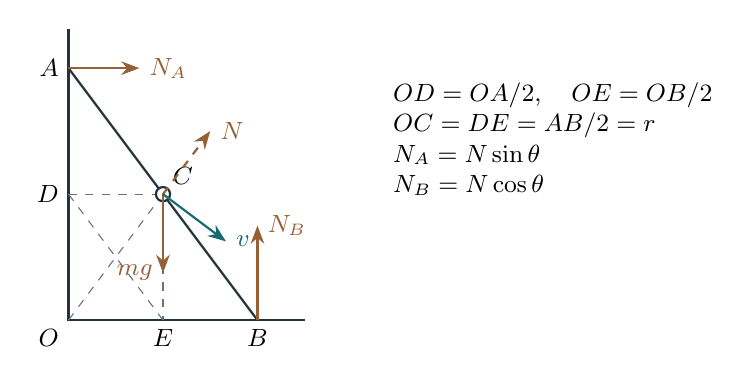
\begin{tikzpicture}
\coordinate(O)at(0,0);\coordinate(A)at(0,3.2);\coordinate(B)at(2.4,0);
\coordinate(C)at(1.2,1.6);\coordinate(D)at(0,1.6);\coordinate(E)at(1.2,0);
\draw[object] (0,3.7)--(O)--(3,0);\draw[object] (A)--(B);
\draw[guide] (D)--(C)--(E);\draw[guide] (D)--(E);\draw[guide] (O)--(C);
\filldraw[object,fill=white] (C) circle(.09);
\foreach \p/\pos in {O/below left,A/left,B/below,C/above right,D/left,E/below}{\node[\pos] at (\p) {$\p$};}
\draw[force] (A)--(.9,3.2) node[right] {$N_A$};
\draw[force] (B)--(2.4,1.2) node[right] {$N_B$};
\draw[force] (C)--(1.2,.6) node[left] {$mg$};
\draw[force,dashed] (C)--(1.8,2.4) node[right] {$N$};
\draw[motion] (C)--(2,1) node[right] {$v$};
\node[align=left,anchor=west] at (4,2.3) {$OD=OA/2,\quad OE=OB/2$\\
$OC=DE=AB/2=r$\\
$N_A=N\sin\theta$\\$N_B=N\cos\theta$};
\end{tikzpicture}
\figcaption{解图3.7B\quad 中点几何决定$C$的轨迹；两支持力的合力可等效移至$C$，并沿$OC$向外。}
\end{minipage}\end{center}

两个支持力的合力方向还可从力矩和分量直接求出。$C$上方的$A$到$C$竖直距离为$r\cos\theta$，
右侧的$B$到$C$水平距离为$r\sin\theta$。
两力的力矩相反，零转动惯量模型要求
$N_A r\cos\theta-N_B r\sin\theta=0$。
因此只要两端仍接触，便有
\[
N_A=N\sin\theta=mg(3\cos\theta-2)\sin\theta,
\quad N_B=N\cos\theta=mg(3\cos\theta-2)\cos\theta.
\]
$0<\theta<\theta_d$内两者非负，在$\theta_d$同时降至零。
若继续强制中心沿圆弧，随后的$3\cos\theta-2<0$就要求墙、地面拉杆，
这与两处只能提供压力的条件不相容。因此圆弧阶段在两支持力共同降为零时结束。脱离瞬间两端仍在接触位置，此后中心沿当时的切线速度进入抛体运动。

图3.7C 说明离位后两端能同时离开接触面。令 $s=OC$，把抛体坐标代入 $s^2=x^2+y^2$。在离位点有 $x_dv_{dx}+y_dv_{dy}=0$ 和 $v_d^2=gy_d$，因此
\[
s^2-r^2=-g v_{dy}\tau^3+\tfrac14g^2\tau^4>0\qquad(\tau>0).
\]
这里 $v_{dy}<0$。在中心触地以前，$x,y$ 均为正，零惯量轻杆可取 $\sin\theta=x/s,\ \cos\theta=y/s$。此时墙端的水平坐标为 $x(1-r/s)>0$，地面端的高度为 $y(1-r/s)>0$，与抛体过程的两个零反力相容。这个取向在离位瞬间接续双接触姿态，因为 $s=r$、$\dot s=0$。有质量的杆还要满足转动方程，其后续姿态和接触力需另求。

\begin{center}\begin{minipage}{.97\linewidth}\centering
\begin{tikzpicture}[scale=.94,transform shape]
\coordinate (O) at (0,0);
\coordinate (C) at (2.07,1.19);
\pgfmathsetmacro{\sC}{sqrt(2.07^2+1.19^2)}
\coordinate (A) at ({2.07*(1-1.56/\sC)},{1.19*(1+1.56/\sC)});
\coordinate (B) at ({2.07*(1+1.56/\sC)},{1.19*(1-1.56/\sC)});
\draw[object](0,2.6)--(O)--(4.45,0);
\draw[guide](0,1.56) arc(90:0:1.56);
\draw[guide](O)--(C) node[pos=.4,below right]{$s$};
\draw[object](A)--(B);
\fill(A)circle(1.6pt)node[above]{$A$};
\fill[accent](C)circle(1.7pt)node[above right]{$C$};
\fill(B)circle(1.6pt)node[above right]{$B$};
\node[below left]at(O){$O$};
\draw[<->] (A)--(0,{1.19*(1+1.56/\sC)});
\draw[<->] (B)--({2.07*(1+1.56/\sC)},0);
\node[align=left,right]at(4.1,1.6){墙端间隙 $x(1-r/s)$\\地面端间隙 $y(1-r/s)$};
\end{tikzpicture}
\figcaption{解图3.7C\quad 离位阶段 $s>r$。图中将两端与墙、地面的间隙放大。}
\end{minipage}\end{center}

\subsubsection*{把落地根式逐步整理}
代入离位竖直速度，有
\[
\begin{aligned}
\tau_{\rm land}
&=\frac{-\sqrt{10gr/27}+\sqrt{46gr/27}}g\\
&=\sqrt{\frac r{27g}}(\sqrt{46}-\sqrt{10})>0.
\end{aligned}
\]
另一根的分子是两个负数之和，对应把抛物线倒推到离位前的数学交点，应舍去。
水平位移中的根式乘法为
\[
\begin{aligned}
v_{dx}\tau_{\rm land}
&=\sqrt{\frac{8gr}{27}}\sqrt{\frac r{27g}}
(\sqrt{46}-\sqrt{10})\\
&=\frac r{27}(\sqrt{368}-\sqrt{80})
=\frac{4r}{27}(\sqrt{23}-\sqrt5).
\end{aligned}
\]
再加上已经走过的$x_d=\sqrt5r/3=9\sqrt5r/27$，
才得到$[5\sqrt5+4\sqrt{23}]r/27$。
最终落点大于离位点的横坐标，却不等于仅有抛体段的水平射程。
全过程中心下降$r$，故碰地前速率平方应为$2gr$；
抛体计算所得$v_x^2=8gr/27$、$v_y^2=46gr/27$的和也为$2gr$，
这与中心从高度 $r$ 降到地面所减少的势能 $mgr$ 一致。


\Needspace{5\baselineskip}

\pdfbookmark[3]{关键洞察}{q7-h5}

\subsection*{关键洞察}

落点坐标是到 $D$ 时已有的水平距离加上随后的抛体位移。零转动惯量使两支持力在 $D$ 同时降到零，图3.7C 说明此后两端都可离开接触面。有质量的杆还受转动方程约束，两个反力的零点可能分开。

\Needspace{5\baselineskip}

\pdfbookmark[3]{易错点}{q7-h6}

\subsection*{易错点}

\begin{itemize}
\item 能量式中的速率是集中质量所在的中心速率。
\item 受约束几何只用到 $D$，之后按脱离速度写抛体。
\item 落点坐标是 $x_d+v_{dx}\tau$，保留 $x_d$。
\item 给杆有限质量时加入转动动能和非零转动惯量，并分别判断两接触力。
\end{itemize}

\Needspace{5\baselineskip}

\pdfbookmark[3]{课堂讲解建议}{q7-h7}

\subsection*{课堂讲解建议}

先在解图3.7B 找出三个中点，问中心到墙角的距离为何恒定，答为直角三角形斜边中点性质。接着在两端标支持力，问它们对中心的力矩为何相抵，答为质量集中在中心、杆的转动惯量为零。到达 $D$ 后，让学生在同一行填写 $x_d,y_d,v_{dx},v_{dy}$，再写抛体方程。求落点时分别指出此前和此后的两段水平位移。

\Needspace{5\baselineskip}

\pdfbookmark[3]{变式训练}{q7-h8}

\subsection*{变式训练}

\begin{enumerate}
\item 将杆长改为 $2L$，仍只在中心集中质量，求落点与全杆长之比。图3.7V1 把中心圆弧半径改为 $L$。脱离初态为 $x_d=\sqrt5L/3,y_d=2L/3,v_{dx}=\sqrt{8gL/27},v_{dy}=-\sqrt{10gL/27}$。由竖直落地正根，$\tau=\sqrt{L/(27g)}(\sqrt{46}-\sqrt{10})$，水平位移为 $4L(\sqrt{23}-\sqrt5)/27$。加上 $x_d$ 后，
\[
\frac{x_P}{2L}=\frac{5\sqrt5+4\sqrt{23}}{54}\approx0.5623.
\]
图中 $D$ 前后两段都按 $L$ 等比例缩放。
\begin{center}\begin{minipage}{.98\linewidth}\centering
\begin{tikzpicture}[scale=0.85,transform shape]
\pgfmathsetmacro{\flightEnd}{(sqrt(46)-sqrt(10))/sqrt(27)}
\draw[axis] (0,0)--(4.55,0) node[right] {$x/L$};\draw[axis] (0,0)--(0,3.65) node[above] {$y/L$};
\draw[traj,domain=0:48.189685,samples=70] plot ({3*sin(\x)},{3*cos(\x)});
\draw[traj,domain=0:\flightEnd,samples=70] plot ({3*(sqrt(5)/3+sqrt(8/27)*\x)},{3*(2/3-sqrt(10/27)*\x-\x^2/2)});
\fill ({sqrt(5)},2) circle (1.7pt) node[above right] {$D$};\fill ({(5*sqrt(5)+4*sqrt(23))/9},0) circle (1.7pt) node[below] {$P$};
\draw[guide] ({sqrt(5)},0)--({sqrt(5)},2);\node[below] at ({sqrt(5)},0) {$\sqrt5/3$};
\end{tikzpicture}
\figcaption{变图3.7V1\quad 全杆长改为 $2L$ 后，中心的圆弧和抛体以 $L$ 为长度单位。}
\end{minipage}\end{center}
\item 用两个支持力分量求脱离角。接触时 $N_A r\cos\theta=N_B r\sin\theta$，故设 $N_A=N\sin\theta,N_B=N\cos\theta$。用中心径向运动求得 $N=mg(3\cos\theta-2)$，于是
\[
N_A=mg(3\cos\theta-2)\sin\theta,\qquad N_B=mg(3\cos\theta-2)\cos\theta.
\]
变图3.7V2 中，两曲线在 $0<\theta<\theta_d$ 均为正，随后在 $\cos\theta_d=2/3$ 共同降为零。这里初始近竖直状态的墙反力也趋零，释放后的有效区间从正的小角开始。
\begin{center}\begin{minipage}{.98\linewidth}\centering
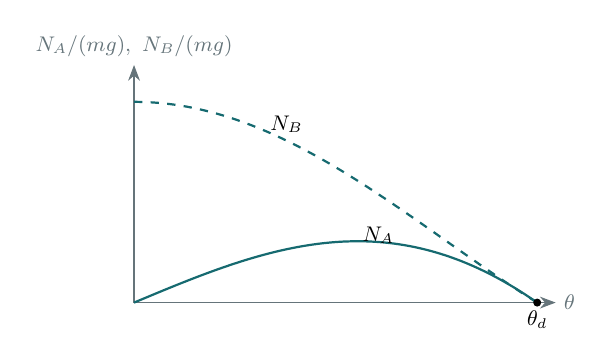
\begin{tikzpicture}[scale=0.85,transform shape]
\draw[axis] (0,0)--(6.3,0) node[right] {$\theta$};\draw[axis] (0,0)--(0,3.55) node[above] {$N_A/(mg),\ N_B/(mg)$};
\draw[traj,domain=0:48.189685,samples=80] plot ({\x/8},{3*(3*cos(\x)-2)*sin(\x)});
\draw[traj,dashed,domain=0:48.189685,samples=80] plot ({\x/8},{3*(3*cos(\x)-2)*cos(\x)});
\fill ({48.189685/8},0) circle (1.7pt) node[below] {$\theta_d$};\node at (2.28,2.66) {$N_B$};\node at (3.65,1.01) {$N_A$};
\end{tikzpicture}
\figcaption{变图3.7V2\quad 轻杆两支持力在同一脱离角降到零。}
\end{minipage}\end{center}
\item 改变中心集中质量，落点怎样变化？能量 $mv^2/2=mgr(1-\cos\theta)$ 中的 $m$ 消去，径向式给出的脱离角也与 $m$ 无关。因而脱离速度、飞行时间及落点保持相同，两个支持力则按 $m$ 成比例改变。变图3.7V3 固定 $\cos\theta=0.8$，有 $N_A=0.24mg,N_B=0.32mg,v/\sqrt{gr}=\sqrt{0.4}$。前两者随质量增加，速率曲线保持水平。
\begin{center}\begin{minipage}{.98\linewidth}\centering
\begin{tikzpicture}[scale=0.85,transform shape]
\draw[axis] (0,0)--(6.6,0) node[right] {$m/m_0$};\draw[axis] (0,0)--(0,3.5) node[above] {归一化量};
\draw[traj,domain=.25:3,samples=45] plot ({2*\x},{3*.24*\x}) node[right] {$N_A/(m_0g)$};
\draw[traj,dashed,domain=.25:3,samples=45] plot ({2*\x},{3*.32*\x}) node[right] {$N_B/(m_0g)$};
\draw[guide] (.5,{3*sqrt(.4)})--(6,{3*sqrt(.4)}) node[right] {$v/\sqrt{gr}$};
\node[below] at (2,0) {$1$};\node[below] at (4,0) {$2$};
\end{tikzpicture}
\figcaption{变图3.7V3\quad 取 $\cos\theta=0.8$。反力与质量成正比，速率由高度决定。}
\end{minipage}\end{center}
\item 给杆均匀质量 $M>0$，中心仍固定质量 $m$，哪些方程要改变？设 $K=m+M$，杆长仍为 $2r$，杆绕中心的转动惯量为 $I=Mr^2/3$。接触阶段中心几何保持，但能量改为 $Kr^2\dot\theta^2/2+I\dot\theta^2/2=Kgr(1-\cos\theta)$。令 $\lambda=K/(K+M/3)$，得
\[
\dot\theta^2=\frac{2\lambda g}r(1-\cos\theta),\qquad \ddot\theta=\frac{\lambda g}r\sin\theta.
\]
运动方程给 $N_A=K\lambda g(3\cos\theta-2)\sin\theta$，$N_B=Kg[1-\lambda(\sin^2\theta+2\cos\theta(1-\cos\theta))]$，力矩为 $rN_B\sin\theta-rN_A\cos\theta=I\ddot\theta$。变图3.7V4取 $M=m$，$\lambda=6/7$。墙反力在 $\cos\theta=2/3$ 消失，此时 $N_B=Kg/7>0$。此后先按仅地面接触的刚体运动求解，中心继续受地面反力，轨迹与前面的轻杆集中质量结果相应改变。
\begin{center}\begin{minipage}{.98\linewidth}\centering
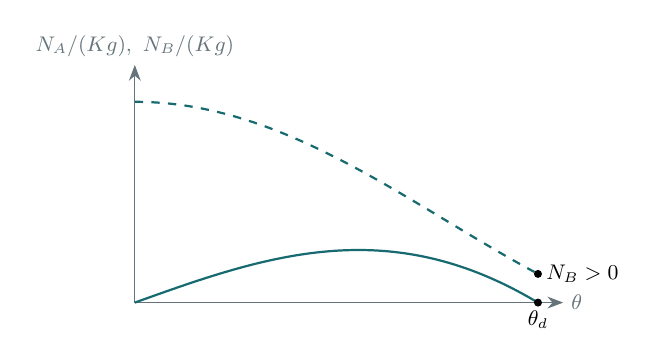
\begin{tikzpicture}[scale=0.85,transform shape]
\draw[axis] (0,0)--(6.4,0) node[right] {$\theta$};\draw[axis] (0,0)--(0,3.55) node[above] {$N_A/(Kg),\ N_B/(Kg)$};
\draw[traj,domain=0:48.189685,samples=82] plot ({\x/8},{3*(6/7)*(3*cos(\x)-2)*sin(\x)});
\draw[traj,dashed,domain=0:48.189685,samples=82] plot ({\x/8},{3*(1-(6/7)*(sin(\x)^2+2*cos(\x)*(1-cos(\x))))});
\coordinate (B) at ({48.189685/8},{3/7});\fill (B) circle (1.7pt) node[right] {$N_B>0$};\fill ({48.189685/8},0) circle (1.7pt) node[below] {$\theta_d$};
\end{tikzpicture}
\figcaption{变图3.7V4\quad 杆质量取为集中质量的同量，墙反力先消失，地面仍有支持。$K=m+M$。}
\end{minipage}\end{center}
\end{enumerate}

\clearpage

\pdfbookmark[2]{第 8 题 轻杆小球跌落与触地速度}{q8}

\section*{第 8 题\quad 轻杆小球跌落与触地速度}

\tagline{M-03-08}

长 $L$ 的理想轻杆，上端固定一质量为 $m$ 的小球，下端支在粗糙水平地面。由近似竖直位置静止释放，球向右下落。设下端在失去地面支持前不滑动（静摩擦系数足够大），杆的质量可忽略。求球第一次碰地前速度的水平、竖直分量；竖直向上取正。

\begin{center}\begin{minipage}{\linewidth}\centering\begin{tikzpicture}
\draw[object](-.7,0)--(3,0);\draw[object](0,0)--(0,2.7);\filldraw[object,fill=white](0,2.7)circle(.14);\node[left]at(0,1.4){$L$};\node[below]at(0,0){$O$};\draw[motion](.3,2.5)--(1,2.3);\node[right]at(.2,2.7){$m$};
\end{tikzpicture}
\figcaption{图 3.8\quad 初始直立状态取无限小扰动的极限。}
\end{minipage}\end{center}

\Needspace{5\baselineskip}

\pdfbookmark[3]{题型定位}{q8-h0}

\subsection*{题型定位}

单侧支点约束下的轻杆集中质量运动。先求圆弧阶段的接触力，确定支持力消失时的速度，再求自由飞行的落地分量。

\Needspace{5\baselineskip}

\pdfbookmark[3]{知识点}{q8-h1}

\subsection*{知识点}

球是唯一有质量的部分，杆保持长度并传递轴向作用力。支点固定时，能量与径向式确定 $v,N$；接触阶段还要满足静摩擦。失去支持后，水平速度保持、竖直速度随重力改变。


\Needspace{5\baselineskip}

\pdfbookmark[3]{物理图像}{q8-h2}

\subsection*{物理图像}

解图3.8A 画初始高度、圆弧脱离点和抛体落点。脱离时切线向右下方，落地时速度更陡。图3.8B 中，球受杆的右上作用，杆受球的左下反作用；地面以向右摩擦与向上支持维持下端静止。

\Needspace{5\baselineskip}

\pdfbookmark[3]{解题入口}{q8-h3}

\subsection*{解题入口}

由 $v^2=2gL(1-\cos\theta)$ 和径向式求 $N=mg(3\cos\theta-2)$，在 $\cos\theta_d=2/3$ 处取切线速度分量。随后保持 $v_x=v_{dx}$，用竖直下降 $2L/3$ 求 $v_y$。同时比较接触阶段的 $f_s/R=\tan\theta$ 与摩擦系数。

\Needspace{5\baselineskip}

\pdfbookmark[3]{标准解法}{q8-h4}

\subsection*{标准解法}

球在支点固定的阶段沿半径$L$的圆弧下落。解图 3.8A 中，失去支持后水平速度保持不变，竖直速度由重力继续改变。
\begin{center}\begin{minipage}{\linewidth}\centering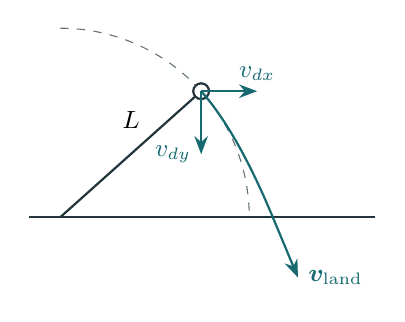
\begin{tikzpicture}
\draw[object](-.4,0)--(4,0);\draw[guide](0,2.4)arc(90:0:2.4);\draw[object](0,0)--(1.789,1.6);\filldraw[object,fill=white](1.789,1.6)circle(.1);\draw[motion](1.789,1.6)--(2.5,1.6)node[above]{$v_{dx}$};\draw[motion](1.789,1.6)--(1.789,.8)node[left]{$v_{dy}$};\draw[traj,domain=0:1,samples=60]plot({1.789+.910*\x},{1.6-1.018*\x-.582*\x^2});
\draw[motion] (2.699,0)--(3.019,-.7673) node[right] {$\vect v_{\mathrm{land}}$};\node[above]at(.9,1){$L$};
\end{tikzpicture}
\figcaption{解图 3.8A\quad 离位时 $\cos\theta_d=2/3$，速度沿切线。}
\end{minipage}\end{center}

\subsubsection*{支点不滑时的圆弧运动}
令杆与竖直方向的夹角为 $\theta$，球位置为 $(L\sin\theta,L\cos\theta)$。支点固定时，杆力沿杆，与球的切线速度垂直，因此不做功。球从高度 $L$ 下降，
\[
v^2=2gL(1-\cos\theta).
\]
设杆对球的作用力 $N$ 沿杆向外为正。径向方程给出
\[
N-mg\cos\theta=-\frac{mv^2}{L},
\qquad N=mg(3\cos\theta-2).
\]
当 $N$ 降为零，地面支持力也降为零。继续沿原圆弧下落会要求地面向下拉杆，故固定支点阶段在这一刻结束，
\[
\cos\theta_d=\frac23,\quad
\sin\theta_d=\frac{\sqrt5}{3},\quad
v_d=\sqrt{\frac{2gL}{3}}.
\]

\subsubsection*{切线分量与自由飞行}
解图 3.8A 中速度指向右下，故
\[
v_{dx}=v_d\cos\theta_d
=\sqrt{\frac{8gL}{27}},\qquad
v_{dy}=-v_d\sin\theta_d
=-\sqrt{\frac{10gL}{27}}.
\]
离位后球仅受重力，水平分量不再变化；竖直方向继续下降 $y_d=2L/3$，所以
\[
v_y^2=v_{dy}^2+2gy_d
=\frac{10gL}{27}+\frac{4gL}{3}
=\frac{46gL}{27}.
\]
碰地前方向向下，应取负根。结果为
\[
\boxed{v_x=\sqrt{\frac8{27}gL},\qquad
v_y=-\sqrt{\frac{46}{27}gL}}.
\]
两分量平方相加得 $v_x^2+v_y^2=2gL$。全过程下降高度 $L$，重力势能减少 $mgL$，正好转为这些动能。

\subsubsection*{不滑动条件}
接触阶段地面所承受的杆力水平、竖直分量分别为 $N\sin\theta,N\cos\theta$，所需静摩擦与支持力之比为 $\tan\theta$。它在这一阶段单调增大，最大值为
\[
\tan\theta_d=\frac{\sqrt5}{2}.
\]
因此题设不滑动可由 $\mu_s\geq\sqrt5/2$ 保证。接触失效时两力同时趋零，以上比值指其左极限。若摩擦不足，支点先滑动，球的圆弧轨迹、离位角和水平速度都需重新求解。
\subsubsection*{把球与支点的受力分别画出}
解图3.8B规定杆力$N$沿杆向外为正。
杆对球的作用力沿右上方；球对杆的反作用力则沿左下方。
无质量杆在接触阶段没有有限的合力与合力矩，
因此地面对杆的向右静摩擦$f_s$与向上支持力$R$分别为
\[
f_s=N\sin\theta,
\qquad R=N\cos\theta.
\]
图3.8B 中，球对杆的水平作用向左，地面对杆的静摩擦因而向右，与该水平分量相抵。
对小球，杆力与切线速度垂直；对杆，地面接触点暂时不动，
所以这两种约束力都不引入额外机械能损失。
\begin{center}\begin{minipage}{\linewidth}\centering
\begin{tikzpicture}
\draw[guide] (0,0)--(1.2,1.2);\filldraw[object,fill=white] (1.2,1.2) circle(.09);
\draw[force] (1.2,1.2)--(1.85,1.85) node[right] {$N$};
\draw[force] (1.2,1.2)--(1.2,-.1) node[right] {$mg$};
\draw[motion] (1.2,1.2)--(1.8,.6) node[right] {$v$};
\node[below] at (.9,-.5) {小球受力};
\draw[object] (4.4,0)--(7,0);\draw[object] (5,0)--(6.2,1.2);
\draw[force] (6.2,1.2)--(5.55,.55) node[above left] {$-N$};
\draw[force] (5,0)--(5,.9) node[left] {$R$};
\draw[force] (5,0)--(5.9,0) node[below] {$f_s$};
\node[below] at (5,-.17) {$O$};\node[below] at (5.7,-.5) {轻杆与地面接触};
\end{tikzpicture}
\figcaption{解图3.8B\quad 作用力与反作用力属于不同物体；支点静摩擦维持的是接触阶段的不滑动。}
\end{minipage}\end{center}

当$N$降到零，$R$与$f_s$同时趋零；继续保持固定支点将需要负的地面支持，因而不再可行。
按理想集中质量轻杆模型，随后小球不受有限的杆力，进入抛体运动。
下端从此随杆移动，$O$ 保留为原支点。理想轻杆采用集中质量极限；若给杆有限质量，杆的转动惯量、动能和接触反力都随之加入运动方程。

\subsubsection*{全程动能与自由飞行中的速度变化}
从初始高度$L$到首次触地，小球的重力势能降低$mgL$，所以
\[
mgL=\frac12m(v_x^2+v_y^2),\qquad v^2=2gL.
\]
离位后没有水平力，故$v_x^2=8gL/27$保持不变；
用全程能量扣除水平动能，直接得到
\[
|v_y|=\sqrt{2gL-\frac{8gL}{27}}
=\sqrt{\frac{46gL}{27}}.
\]
落地时竖直分量向下，按题设正向取$v_y<0$。
全程能量给碰地前的总速率。水平方向的速度由离位前的圆弧速率和切线投影求出；保留这一分量后，剩余的动能才给竖直速度大小。

从离位时的高度和竖直初速度，也可求自由飞行时间：
\[
\tau=\frac{v_{dy}+\sqrt{v_{dy}^2+2g(2L/3)}}g
=\sqrt{\frac L{27g}}(\sqrt{46}-\sqrt{10}).
\]
代入$v_y=v_{dy}-g\tau$，$\sqrt{10gL/27}$两项抵消，
仍得到负的$\sqrt{46gL/27}$。解图3.8A中起点箭头为离位速度分量，
落点的斜箭头为碰地前速度；水平分量相同，竖直分量的绝对值已经增加。


\Needspace{5\baselineskip}

\pdfbookmark[3]{关键洞察}{q8-h5}

\subsection*{关键洞察}

固定下端是第一段的接触条件。支持力与摩擦力共同降为零后，球从既有的位置和切线速度进入自由飞行。若摩擦先达到上限，下端会先滑，圆弧阶段相应提前结束。

\Needspace{5\baselineskip}

\pdfbookmark[3]{易错点}{q8-h6}

\subsection*{易错点}

\begin{itemize}
\item 能量只计小球的动能，速率为 $L\dot\theta$。
\item 离位竖直分量为 $-\sqrt{10gL/27}$，落地前还经重力加速。
\item $f_s/R=\tan\theta$ 随下落增大，维持到离位需 $\mu_s\geq\sqrt5/2$。
\item 各速度分量的单位都是 $\sqrt{gL}$，落地竖直速度按向上正向取负值。
\end{itemize}

\Needspace{5\baselineskip}

\pdfbookmark[3]{课堂讲解建议}{q8-h7}

\subsection*{课堂讲解建议}

在解图3.8A 分别标出离位和落地两个速度箭头，问它们的哪个分量相同，答为水平分量。再问竖直分量相差多少动能，由下降高度 $2L/3$ 读出 $\Delta(v_y^2)=4gL/3$。在图3.8B 中先画球对杆的反作用，再确定地面摩擦方向。最后用变图3.8V3 标出给定 $\mu_s$ 的滑动角，比较它与离位角，说明题设摩擦假定对应哪一段过程。

\Needspace{5\baselineskip}

\pdfbookmark[3]{变式训练}{q8-h8}

\subsection*{变式训练}

\begin{enumerate}
\item 求球的水平落点。由脱离点 $x_d=\sqrt5L/3$ 和水平速度 $v_{dx}=\sqrt{8gL/27}$，竖直方程给 $\tau=\sqrt{L/(27g)}(\sqrt{46}-\sqrt{10})$。变图3.8V1 中，$D$ 到 $P$ 的水平距离为 $v_{dx}\tau=4L(\sqrt{23}-\sqrt5)/27$，所以
\[
x_P=x_d+v_{dx}\tau=\frac{5\sqrt5+4\sqrt{23}}{27}L.
\]
图中两段标尺分别量此前的位移和脱离后的位移。
\begin{center}\begin{minipage}{.98\linewidth}\centering
\begin{tikzpicture}[scale=0.85,transform shape]
\pgfmathsetmacro{\flightEnd}{(sqrt(46)-sqrt(10))/sqrt(27)}
\draw[axis] (0,0)--(4.65,0) node[right] {$x/L$};\draw[axis] (0,0)--(0,3.6) node[above] {$y/L$};
\draw[traj,domain=0:48.189685,samples=70] plot ({3*sin(\x)},{3*cos(\x)});
\draw[traj,domain=0:\flightEnd,samples=70] plot ({3*(sqrt(5)/3+sqrt(8/27)*\x)},{3*(2/3-sqrt(10/27)*\x-\x^2/2)});
\fill ({sqrt(5)},2) circle (1.6pt) node[above right] {$D$};\fill ({(5*sqrt(5)+4*sqrt(23))/9},0) circle (1.6pt) node[below right] {$P$};
\draw[guide] ({sqrt(5)},0)--({sqrt(5)},2);\draw[axis,<->] (0,-.75)--({sqrt(5)},-.75) node[midway,below] {$x_d/L$};
\draw[axis,<->] ({sqrt(5)},-.75)--({(5*sqrt(5)+4*sqrt(23))/9},-.75) node[midway,below] {$\Delta x/L$};
\end{tikzpicture}
\figcaption{变图3.8V1\quad 落点横坐标由圆弧和自由飞行两段的水平位移组成。}
\end{minipage}\end{center}
\item 直接从竖直运动求落地速度。脱离后下降距离为 $s$ 时，$v_y^2=v_{dy}^2+2gs$，其中 $v_{dy}^2=10gL/27$。变图3.8V2 的直线起于 $D$，在 $s/L=2/3$ 到达 $P$，故 $v_y^2/(gL)=10/27+4/3=46/27$。该段一直向下，取 $v_y=-\sqrt{46gL/27}$。水平分量保持 $\sqrt{8gL/27}$，两分量平方和为 $2gL$。
\begin{center}\begin{minipage}{.98\linewidth}\centering
\begin{tikzpicture}[scale=0.85,transform shape]
\draw[axis] (0,0)--(5.2,0) node[right] {$s/L$};\draw[axis] (0,0)--(0,3.8) node[above] {$v_y^2/(gL)$};
\draw[traj] (0,{2*10/27})--(4,{2*46/27});\draw[guide] (4,0)--(4,{2*46/27})--(0,{2*46/27});
\fill (0,{2*10/27}) circle (1.6pt) node[right] {$D$};\fill (4,{2*46/27}) circle (1.6pt) node[above right] {$P$};
\node[left] at (0,{2*10/27}) {$10/27$};\node[left] at (0,{2*46/27}) {$46/27$};\node[below] at (4,0) {$2/3$};
\end{tikzpicture}
\figcaption{变图3.8V2\quad 自由飞行中，竖直速度平方随下降距离线性增长。}
\end{minipage}\end{center}
\item 静摩擦系数小于 $\sqrt5/2$ 时，先发生哪种约束变化？固定支点阶段有 $f_s/R=\tan\theta$，它从零随 $\theta$ 增加。静摩擦达到上限时 $\tan\theta_s=\mu_s$。因此 $0\leq\mu_s<\sqrt5/2$ 对应 $\theta_s<\theta_d$，支点先滑动。变图3.8V3 取 $\mu_s=0.5$，在 $S$ 处 $\theta_s\approx26.565^\circ$，早于离位角约 $48.190^\circ$。此时 $3\cos\theta_s-2>0$，地面仍有正支持，后续需在滑动接触条件下重新求球与杆的运动。
\begin{center}\begin{minipage}{.98\linewidth}\centering
\begin{tikzpicture}[scale=0.85,transform shape]
\draw[axis] (0,0)--(6.5,0) node[right] {$\theta$};\draw[axis] (0,0)--(0,3.45) node[above] {$f_s/R$};
\draw[traj,domain=0:48.189685,samples=82] plot ({\x/8},{2.5*tan(\x)});
\draw[guide] (0,1.25)--({atan(.5)/8},1.25)--({atan(.5)/8},0);
\fill ({atan(.5)/8},1.25) circle (1.6pt) node[above left] {$S$};\fill ({48.189685/8},{2.5*sqrt(5)/2}) circle (1.6pt) node[above left] {$D$};
\node[left] at (0,1.25) {$\mu_s=0.5$};\node[below] at ({atan(.5)/8},0) {$\theta_s$};\node[below] at ({48.189685/8},0) {$\theta_d$};
\end{tikzpicture}
\figcaption{变图3.8V3\quad 摩擦不足时，固定支点过程先在 $S$ 结束；$D$ 是足够摩擦下的离位点。}
\end{minipage}\end{center}
\item 地面改为完全光滑，写水平动量条件并说明集中质量极限的运动。地面只有竖直支持力，系统水平动量守恒。理想轻杆只含球的质量，从静止释放便有 $m\dot x_P=0$。对于有小倾角的直杆，杆端竖直力与上端轴向力要同时满足零合力和零力矩，二者均为零，球由重力作竖直自由落体。变图3.8V4取初始小角 $\theta_i>0$，有
\[
x_P=L\sin\theta_i,\quad y_P=L\cos\theta_i-gt^2/2,\quad x_B=x_P-\sqrt{L^2-y_P^2}.
\]
球下降时，下端 $B$ 向左移动以保持杆长。取 $\theta_i\to0^+$ 的近竖直极限，首次触地前 $v_x\to0$、$v_y\to-\sqrt{2gL}$。若给杆有限质量 $M$，水平动量改为 $m\dot x_P+M\dot x_C=0$，并加入杆的平动、转动动能后求解。
\begin{center}\begin{minipage}{.98\linewidth}\centering
\begin{tikzpicture}[scale=0.85,transform shape]
\draw[object] (-2.5,0)--(3.6,0);\coordinate (P0) at (1.1,3);\coordinate (B0) at (0,0);\coordinate (P1) at (1.1,1.5);\coordinate (B1) at ({1.1-sqrt(1.1^2+3^2-1.5^2)},0);
\draw[object,dashed] (B0)--(P0);\draw[object] (B1)--(P1);\draw[guide] (P0)--(1.1,0);
\fill (P0) circle (2pt) node[above] {$P_i$};\fill (P1) circle (2pt) node[right] {$P$};\fill (B0) circle (1.6pt) node[below] {$B_i$};\fill (B1) circle (1.6pt) node[below] {$B$};
\draw[motion] (P1)--(1.1,.45) node[right] {$\vect v_P$};\draw[motion] (-.25,-.52)--(-1.4,-.52) node[below] {下端滑动};
\end{tikzpicture}
\figcaption{变图3.8V4\quad 光滑地面的集中质量极限，球沿竖直线下降，下端向左移动。}
\end{minipage}\end{center}
\end{enumerate}

\clearpage

\pdfbookmark[2]{第 9 题 绳绕钉运动与碰钉条件}{q9}

\section*{第 9 题\quad 绳绕钉运动与碰钉条件}

\tagline{M-03-09}

长 $2l$ 的理想细绳，一端固定在钉子 $A$，另一端系小球。小球初始位于 $A$ 右侧同一水平线上，以竖直向下初速度 $v_0$ 运动。钉子 $B$ 位于 $A$ 左侧，$AB=l$。绳转到 $B$ 后，小球绕 $B$ 上行。求小球直接碰到 $A$ 所需的最小初速，允许松绳后以抛体轨迹命中。

\begin{center}\begin{minipage}{\linewidth}\centering\begin{tikzpicture}
\fill(0,0)circle(2pt);\fill(-1.5,0)circle(2pt);\draw[object](0,0)--(3,0);\filldraw[object,fill=white](3,0)circle(.1);\node[above]at(0,0){$A$};\node[above]at(-1.5,0){$B$};\draw[motion](3,0)--(3,-1)node[right]{$v_0$};\draw[guide](3,0)arc(0:-180:3);\draw[<->](-1.5,.65)--(0,.65)node[midway,above]{$l$};
\end{tikzpicture}
\figcaption{图 3.9\quad 先绕 $A$ 经过下半圆，再绕 $B$ 向上运动。}
\end{minipage}\end{center}

\Needspace{5\baselineskip}

\pdfbookmark[3]{题型定位}{q9-h0}

\subsection*{题型定位}

绕钉后圆周约束和松绳抛体的衔接。碰到钉子时半径从 $2l$ 改为 $l$，同高度的速度连续。随后按张力的首次零点确定发射点，并比较两条直接命中路径的初始能量。

\Needspace{5\baselineskip}

\pdfbookmark[3]{知识点}{q9-h1}

\subsection*{知识点}

能量守恒、径向张力、切线发射、目标位移和绳长不等式。松绳时保留连续的位置和速度，之后用同一飞行时间描述目标位置与球到新圆心的距离。


\Needspace{5\baselineskip}

\pdfbookmark[3]{物理图像}{q9-h2}

\subsection*{物理图像}

图3.9 的小球先绕 $A$ 下行，到左端时绳中点接触 $B$，竖直向上的速度同时垂直于两个共线半径。解图3.9A 的 $D$ 位于 $B$ 左上方，发射速度向右上，球在绳长圆内飞行至 $A$。解图3.9B 的张力曲线在速度仍大于零时先到横轴，确定圆周运动结束的位置。

\Needspace{5\baselineskip}

\pdfbookmark[3]{解题入口}{q9-h3}

\subsection*{解题入口}

先以能量求球到左端的速度，再以半径 $l$ 写上行段 $v^2=v_0^2-2gl\sin\theta$ 和 $T_B=mv_0^2/l-3mg\sin\theta$。首次张力零点给 $v^2=gl\sin\theta$。把 $D=(-l\cos\theta,l\sin\theta)$ 的切线速度投到水平和竖直方向，用同一时间到达 $A=(l,0)$，消元求松绳角。最后比较完整上半圆的阈值，并计算松绳后的径向距离。

\Needspace{5\baselineskip}

\pdfbookmark[3]{标准解法}{q9-h4}

\subsection*{标准解法}

小球到 $A$ 左侧 $2l$ 处时速度仍为 $v_0$。改绕 $B$ 后，令松绳点 $D=(-l\cos\theta,l\sin\theta)$（以 $B$ 为原点），如解图 3.9A。
\begin{center}\begin{minipage}{\linewidth}\centering\begin{tikzpicture}
\draw[guide](-1.5,0)arc(180:0:1.5);\fill(0,0)circle(2pt);\fill(1.5,0)circle(2pt);\node[below]at(0,0){$B$};\node[below]at(1.5,0){$A$};\coordinate(D)at(-.75,1.299);\draw[object](0,0)--(D);\fill(D)circle(2pt);\node[above left]at(D){$D$};\draw[motion](D)--(-.1,1.674)node[above]{$v$};\draw[traj,domain=0:2.25,samples=40]plot({-.75+\x},{1.299+.57735*\x-.5132*\x^2});\draw(-.5,0)arc(180:120:.5);\node at(-.6,.35){$\theta$};
\end{tikzpicture}
\figcaption{解图 3.9A\quad 最小初速对应 $\theta=60^\circ$ 时松绳，随后命中 $A$。}
\end{minipage}\end{center}

\subsubsection*{绕钉前后的能量}
小球先绕 $A$ 走下半圆，到达 $A$ 左侧同高位置时，速率又为 $v_0$；这一阶段绳张力为正。绳接触 $B$ 后，有效半径变为 $l$。
以 $B$ 为原点，令球在上行段的位置为
\[
(x,y)=(-l\cos\theta,l\sin\theta),\quad 0<\theta<\pi.
\]
在从左端上升到松绳点的阶段，
\[
v^2=v_0^2-2gl\sin\theta.
\]
指向 $B$ 的重力分量为 $mg\sin\theta$，径向方程是
\[
T+mg\sin\theta=\frac{mv^2}{l}.
\]
因此 $T=0$ 时有 $v^2=gl\sin\theta$，与能量式联立：
\[
v_0^2=3gl\sin\theta.
\]

\subsubsection*{抛体经过目标的条件}
若在上升到最高点之前松绳，$0<\theta<\pi/2$，其切线速度为 $(v\sin\theta,v\cos\theta)$。如解图 3.9A，目标 $A=(l,0)$，故
\[
l=-l\cos\theta+v\sin\theta\,\tau,
\]
\[
0=l\sin\theta+v\cos\theta\,\tau-\frac12g\tau^2.
\]
第一式给出 $\tau=l(1+\cos\theta)/(v\sin\theta)>0$。代入第二式，再代入 $v^2=gl\sin\theta$，约去非零因子后得到
\[
1-3\cos^2\theta-2\cos^3\theta=0.
\]
等价地，
\[
(2\cos\theta-1)(\cos\theta+1)^2=0.
\]
符合上行松绳范围的根只有 $\cos\theta=1/2$，即 $\theta=60^\circ$。于是
\[
\boxed{v_{0,\min}=\sqrt{\frac{3\sqrt3}{2}\,gl}}.
\]

\subsubsection*{两条命中路径与绳长条件}
若全程张紧经过绕 $B$ 的上半圆，最高点要求 $v_{\mathrm{top}}^2\geq gl$，所以 $v_0^2\geq3gl$，所需初速更大。小于抛体命中值的初速又不能满足上述唯一的命中根，因此所得初速是最小值。

松绳后，球到 $B$ 的距离至多为 $l$，因此还要沿这段抛体轨道计算到 $B$ 的距离。令 $z=v\tau/l$，在 $\theta=60^\circ$ 的轨道上，
\[
\frac{x}{l}=-\frac12+\frac{\sqrt3}{2}z,\qquad
\frac{y}{l}=\frac{\sqrt3}{2}+\frac12z-\frac{z^2}{\sqrt3}.
\]
从松绳到命中，$0\leq z\leq\sqrt3$，直接计算
\[
\frac{x^2+y^2}{l^2}-1=\frac{z^3(z-\sqrt3)}3\leq0.
\]
球始终位于以 $B$ 为圆心、半径 $l$ 的圆内，直到目标处才再次达到绳长。因此这段抛体轨道与松绳约束相容。
\subsubsection*{绕钉前后的张力及首次松绳位置}
先写绕$A$下半圆时的速率和张力。以初始水平线为势能零点，
令该段位置角$\gamma$从右端沿顺时针量起，$0\leq\gamma\leq\pi$。
球的高度为$-2l\sin\gamma$，能量与径向方程分别给出
\[
v_A^2=v_0^2+4gl\sin\gamma,
\qquad T_A-mg\sin\gamma=\frac{mv_A^2}{2l},
\]
所以$T_A=mv_0^2/(2l)+3mg\sin\gamma>0$。
该段不会先松绳，到左端时$\sin\gamma=0$，速率确实回到$v_0$，方向竖直向上。
绳的中点在这一刻碰到$B$，速度与新半径仍然垂直，因此不需要切向冲量，也没有动能突失。

绕$B$上行后，张力随位置变化的完整函数是
\[
T_B=\frac m l(v_0^2-2gl\sin\theta)-mg\sin\theta
=\frac{mv_0^2}{l}-3mg\sin\theta.
\]
若$0<v_0^2<3gl$，从$\theta=0$开始张力为正，随上升不断减小，
第一次到零满足$\sin\theta=v_0^2/(3gl)$。
同一圆周公式的速度零点由能量式给出，应有$\sin\theta=v_0^2/(2gl)$，
其值更大，所以球先到张力零点，再转入自由飞行。图B 的圆周公式在张力零点后改用虚线表示延长的数值。
解图3.9B将速度平方与张力同时画出，松绳处的速率仍不为零。
\begin{center}\begin{minipage}{\linewidth}\centering
\begin{tikzpicture}[x=4cm,y=1.05cm]
\draw[axis] (-.05,0)--(1.22,0) node[right] {$u=\sin\theta$};
\draw[axis] (0,-.5)--(0,2.95) node[above] {归一化量};
\draw[traj,domain=0:.866025] plot(\x,{2.598076-2*\x});
\draw[force,domain=0:.866025] plot(\x,{2.598076-3*\x});
\draw[traj,dashed,domain=.866025:1] plot(\x,{2.598076-2*\x});
\draw[force,dashed,domain=.866025:1] plot(\x,{2.598076-3*\x});
\draw[guide] (.866025,0)--(.866025,.866025);
\fill (.866025,0) circle(1.7pt);\fill (.866025,.866025) circle(1.7pt);
\node[above] at (.5,1.598076) {$v^2/(gl)$};
\node[below left] at (.5,1.098076) {$T_B/(mg)$};
\node[below] at (.866025,-.05) {$\sqrt3/2$};
\node[align=left] at (1.8,1.8) {$v_0^2/(gl)=3\sqrt3/2$\\
实线：张紧阶段\\虚线：同一圆周公式的延拓\\松绳时$v^2/(gl)=\sqrt3/2$};
\end{tikzpicture}
\figcaption{解图3.9B\quad 张力为零时转入抛体，实线给出张紧阶段，虚线是圆周公式的延长值。}
\end{minipage}\end{center}

\subsubsection*{以松绳点为原点的目标位移与命中方程}
也可把坐标原点移至松绳点$D$。此时目标位移为
\[
X_A=l(1+\cos\theta),\qquad Y_A=-l\sin\theta.
\]
发射速度与水平正向的夹角为$\alpha=\pi/2-\theta$，
故$\tan\alpha=\cot\theta$、$v\cos\alpha=v\sin\theta$。
从参数式消去时间，得到
\[
Y=X\cot\theta-\frac{gX^2}{2v^2\sin^2\theta}.
\]
将目标坐标和$v^2=gl\sin\theta$全部代入，逐项除以$l$，有
\[
-\sin\theta=\frac{(1+\cos\theta)\cos\theta}{\sin\theta}
-\frac{(1+\cos\theta)^2}{2\sin^3\theta}.
\]
以 $D$ 为原点时，目标在 $D$ 下方，$Y_A=-l\sin\theta$。以 $B$ 为原点时目标高度为零，两者相差的量就是 $D$ 的高度。
令$c=\cos\theta$，乘以$2\sin^3\theta$后整理：
\[
2(1-c^2)^2+2c(1+c)(1-c^2)-(1+c)^2
=1-3c^2-2c^3=0.
\]
等价多项式为$2c^3+3c^2-1$，
把 $(2c-1)(c+1)^2$ 乘开，三次、二次和常数项分别为 $2c^3,3c^2,-1$。
上行段在最高点前松绳，对应 $0<c<1$。其中唯一的根是 $c=1/2$，另一个代数根 $c=-1$ 位于该区间之外，且使消元所除的 $\sin\theta$ 为零。
有效根$c=1/2$使飞行时间为正，与前面以$B$为原点的计算相同。

最后比较两条直接命中路径。全程张紧时，
$T_B$在上半圆最高点最小，要求$v_0^2\geq3gl$；
先松绳再直接命中只需$v_0^2=(3\sqrt3/2)gl$，
二者的初动能比为$\sqrt3/2<1$。
在低于完整半圆阈值的首次上行过程中，松绳点由初速唯一确定，
命中方程又只允许$60^\circ$这一有效角度，故更小的初速不能沿这段自由飞行直接命中$A$。
距离不等式给出整段自由飞行都在可用绳长内，所以这条命中路径实际可达。
在最小初速轨道上，飞行参数还可具体写成
$v=v_0/\sqrt3$、$\tau=\sqrt3l/v=3l/v_0$。
抛体最高点由竖直速度降为零确定，其坐标为
$(-l/8,9\sqrt3l/16)$，最大高度仍小于绕$B$圆周的最高点$l$。
小球保留向右的水平速度，因此不必先升到圆周顶部也能越到目标$A$。
这条轨道保留向右的水平运动，所需初动能较小。图中$D$位于$B$的左上方，对应从左端上行过程中张力第一次降为零的位置。



\Needspace{5\baselineskip}

\pdfbookmark[3]{关键洞察}{q9-h5}

\subsection*{关键洞察}

半径改变使所需向心加速度改变，切线速度和动能在理想绕钉瞬间连续。最小初速对应的轨道先失去张力，再利用向右的水平速度命中目标，球的最高点低于绕 $B$ 的圆周最高点。

\Needspace{5\baselineskip}

\pdfbookmark[3]{易错点}{q9-h6}

\subsection*{易错点}

\begin{itemize}
\item 绕钉瞬间的速度方向与新半径垂直，接续的能量式取同一速度。
\item 绕 $B$ 的半径取剩下的绳长 $l$，张力条件按新半径重列。
\item 全程张紧分支的最高点满足 $T_B\geq0$，松绳分支用 $T_B=0$ 接续抛体。
\item 目标命中前到 $B$ 的距离应在允许绳长内，同一飞行参数用于位置和距离。
\end{itemize}

\Needspace{5\baselineskip}

\pdfbookmark[3]{课堂讲解建议}{q9-h7}

\subsection*{课堂讲解建议}

先在题图的左端画速度箭头，问“绳碰到 $B$ 后，这支箭头是否仍垂直于新半径？”它仍竖直向上，动能连续。再沿解图3.9B 读张力零点，指出此时速率仍为正。让学生在变图V2 标目标相对 $D$ 的负竖直位移，再用水平位移除水平速度求飞行时间。最后对比变图V3 的两根能量柱，并用圆内距离式说明较低能量的抛体轨道在命中前保持松绳。

\Needspace{5\baselineskip}

\pdfbookmark[3]{变式训练}{q9-h8}

\subsection*{变式训练}

\begin{enumerate}
\item 求最小初速轨道从松绳到命中的时间。在 $\theta=60^\circ$ 的 $D$ 点，水平速度为 $v\sin60^\circ=\sqrt3v/2$，变图V1 的水平位移为 $3l/2$，所以
\[
\tau=\frac{3l/2}{\sqrt3v/2}=\frac{\sqrt3l}{v},\qquad v^2=\frac{\sqrt3}{2}gl.
\]
由 $v_0^2=3v^2$ 也可写成 $\tau=3l/v_0$。竖直位移等于 $v\cos60^\circ\tau-g\tau^2/2=-\sqrt3l/2$，恰好从 $D$ 降到目标水平线。
\begin{center}\begin{minipage}{.98\linewidth}\centering
\begin{tikzpicture}[scale=.88,transform shape]
\draw[guide] (0,0) circle (1.55);
\coordinate (B) at (0,0);\coordinate (A) at (1.55,0);\coordinate (D) at (-.775,1.34234);
\draw[traj,domain=0:1.73205,samples=100] plot({1.55*(-.5+.8660254*\x)},{1.55*(.8660254+.5*\x-\x^2/1.7320508)});
\fill (B) circle(1.55pt) node[below] {$B$};\fill (A) circle(1.55pt) node[below] {$A$};
\fill (D) circle(1.55pt) node[above left] {$D$};
\draw[motion] (D)--++(.8054,.465) node[above] {$v$};
\draw[<->] (-.775,-.5)--(1.55,-.5) node[midway,below] {$3l/2$};
\draw[guide] (D)--(-.775,-.5);
\draw[guide] (A)--(1.55,-.5);
\end{tikzpicture}
\figcaption{变图3.9V1\quad 水平位移除以恒定水平速度，给出从松绳到命中的时间。}
\end{minipage}\end{center}
\item 把松绳点 $D$ 作为坐标原点重新消元。目标位移为 $X_A=l(1+\cos\theta)$、$Y_A=-l\sin\theta$。水平速度是 $v\sin\theta$，故 $\tau=X/(v\sin\theta)$。代入竖直位移式，得
\[
Y=X\cot\theta-\frac{gX^2}{2v^2\sin^2\theta}.
\]
把 $X_A,Y_A$ 和 $v^2=gl\sin\theta$ 代入，乘 $2\sin^3\theta/l$ 后，令 $c=\cos\theta$，整理为 $1-3c^2-2c^3=0$。在 $0<c<1$ 上有效根为 $c=1/2$。图V2 画出这个根对应的位移轨道，终点纵坐标为 $-\sqrt3/2$。
\begin{center}\begin{minipage}{.98\linewidth}\centering
\begin{tikzpicture}[scale=.88,transform shape]
\draw[axis] (0,0)--(3.65,0) node[right] {$X/l$};
\draw[axis] (0,-2.2)--(0,1.15) node[above] {$Y/l$};
\draw[traj,domain=0:1.5,samples=100] plot({2*\x},{2*(\x/1.7320508-4*\x^2/(3*1.7320508))});
\coordinate (A) at (3,-1.73205);
\draw[guide] (A)--(3,0) node[above] {$3/2$};
\draw[guide] (A)--(0,-1.73205) node[left] {$-\sqrt3/2$};
\fill (0,0) circle(1.6pt) node[above left] {$D$};\fill (A) circle(1.6pt) node[below right] {$A$};
\draw[motion] (0,0)--(1.05,.6062) node[above] {$v$};
\end{tikzpicture}
\figcaption{变图3.9V2\quad 把松绳点作为原点，目标的竖直位移为负。}
\end{minipage}\end{center}
\item 比较全程张紧的上半圆和松绳后命中所需的初动能。前者在最高点满足 $v_{\rm top}^2\geq gl$，从左端到最高点上升 $l$，故初速平方至少为 $3gl$，初动能至少为 $3mgl/2$。后者由松绳角 $60^\circ$ 得初动能 $3\sqrt3mgl/4$。图V3 两柱高度之比为 $\sqrt3/2$。松绳轨道的水平速度使球在低于圆顶的高度越向 $A$，所以初动能较小。
\begin{center}\begin{minipage}{.98\linewidth}\centering
\begin{tikzpicture}[scale=.88,transform shape]
\draw[axis] (0,0)--(6.1,0);
\draw[axis] (0,0)--(0,3.25) node[above] {$E_0/(mgl)$};
\filldraw[object,fill=accent!20] (1,0) rectangle (2.2,2.59808);
\filldraw[object,fill=warm!20] (3.7,0) rectangle (4.9,3);
\node[above] at (1.6,2.59808) {$3\sqrt3/4$};
\node[above] at (4.3,3) {$3/2$};
\node[below] at (1.6,0) {松绳后命中};
\node[below] at (4.3,0) {全程张紧};
\end{tikzpicture}
\figcaption{变图3.9V3\quad 两条可行路径的初动能分别为 $3\sqrt3mgl/4$ 和 $3mgl/2$。}
\end{minipage}\end{center}
\item 把 $AB$ 改为 $\eta l$，保持总绳长 $2l$，建立新的命中条件。取 $0<\eta<2$，绕 $B$ 的半径为 $r=(2-\eta)l$，目标为 $A=(\eta l,0)$。按图V4 设 $D=(-r\cos\theta,r\sin\theta)$，能量与张力零点给 $v_0^2=3gr\sin\theta$、$v^2=gr\sin\theta$。写 $u=\eta/(2-\eta)$，以 $z=v\tau/r$ 描述飞行，
\[
x/r=-\cos\theta+z\sin\theta,\qquad
y/r=\sin\theta+z\cos\theta-\frac{z^2}{2\sin\theta}.
\]
命中要求 $z_A=(u+\cos\theta)/\sin\theta$ 且 $y(z_A)=0$，等价于 $2u\cos^3\theta+3\cos^2\theta+u^2-2=0$。同时沿 $0\leq z\leq z_A$ 保持
\[
\frac{x^2+y^2}{r^2}-1=\frac{z^3(z-4\sin\theta\cos\theta)}{4\sin^2\theta}\leq0 .
\]
命中时有 $y=0$、$x=ur$，所以保持短段绳松弛要求 $u\leq1$，即 $0<\eta\leq1$。在这段参数范围，命中方程的左端在 $c=\cos\theta=0$ 时为 $u^2-2<0$，在 $c=1$ 时为 $(u+1)^2>0$，并随 $c$ 增大，故只有一个有效根。命中点已经在圆内或圆上，距离式给出 $z_A\leq4\sin\theta\cos\theta$，从而在此之前的每个时刻都还处在圆内。图V4 取 $\eta=4/5$ 作例。$\eta=1$ 时目标落在圆周，回到主问题；$\eta>1$ 时目标移到短段绳的圆外，沿这段松绳抛物线将先碰到圆周。
\begin{center}\begin{minipage}{.98\linewidth}\centering
\begin{tikzpicture}[scale=.88,transform shape]
\pgfmathsetmacro{\CosD}{0.6358260539}
\pgfmathsetmacro{\SinD}{sqrt(1-\CosD^2)}
\pgfmathsetmacro{\flight}{(2/3+\CosD)/\SinD}
\pgfmathsetmacro{\angleD}{acos(\CosD)}
\draw[guide] (-1.8,0) arc(180:0:1.8);
\draw[guide] (-1.88,0)--(1.85,0);
\coordinate (D) at ({-1.8*\CosD},{1.8*\SinD});
\draw[traj,domain=0:\flight,samples=75] plot({1.8*(-\CosD+\x*\SinD)},{1.8*(\SinD+\x*\CosD-\x^2/(2*\SinD))});
\fill (0,0) circle(1.6pt) node[below left] {$B$};
\fill (1.2,0) circle(1.6pt) node[above right] {$A$};
\fill (D) circle(1.6pt) node[above left] {$D$};
\draw[object] (0,0)--(D) node[midway,above left] {$r$};
\draw[<->] (0,-.55)--(1.2,-.55) node[midway,below] {$\eta l$};
\draw[motion] (D)--++({.86*\SinD},{.86*\CosD}) node[above left] {$v$};
\draw[object] (-.48,0) arc[start angle=180,end angle={180-\angleD},radius=.48];
\node at (-.61,.20) {$\theta$};
\node[right] at (2.02,1.05) {$\eta=4/5$};
\end{tikzpicture}
\figcaption{变图3.9V4\quad 取 $\eta=4/5$。$D$ 的抛物线在半径 $r=(2-\eta)l$ 的圆内经过 $A$。}
\end{minipage}\end{center}
\end{enumerate}

\clearpage

\pdfbookmark[2]{第 10 题 引力追及中的最大间距}{q10}

\section*{第 10 题\quad 引力追及中的最大间距}

\tagline{M-03-10}

惯性系 $S$ 中，质量分别为 $m_1,m_2$ 的质点 $A,B$ 以万有引力相互吸引。起初 $A$ 静止，间距 $l_0$；$B$ 沿连线远离 $A$，速度 $v_0<\sqrt{2Gm_2/l_0}$。外力 $F$ 始终作用于 $B$，使其速度保持 $v_0$。求两点最大间距及达到该间距前外力在 $S$ 中所做的功。

\begin{center}\begin{minipage}{\linewidth}\centering\begin{tikzpicture}
\fill(0,0)circle(3pt);\fill(3,0)circle(3pt);\node[below]at(0,0){$A,m_1$};\node[below]at(3,0){$B,m_2$};\draw[motion](3,.4)--(4.2,.4)node[right]{$v_0$};\draw[force](3,-.4)--(4.2,-.4)node[right]{$F$};\draw[<->](0,.9)--(3,.9)node[midway,above]{$l_0$};
\end{tikzpicture}
\figcaption{图 3.10\quad $F$ 抵消 $B$ 所受引力，$A$ 则不断加速。}
\end{minipage}\end{center}

\Needspace{5\baselineskip}

\pdfbookmark[3]{题型定位}{q10-h0}

\subsection*{题型定位}

受控匀速引力源与追及运动。用随 $B$ 平移的惯性系求最大间距，再在指定系求维持 $B$ 匀速的外力功。

\Needspace{5\baselineskip}

\pdfbookmark[3]{知识点}{q10-h1}

\subsection*{知识点}

相对速度、引力势能、质点系机械能增量、外力冲量和功的参考系变换。最大间距处 $\dot l=0$，所以 $A,B$ 在 $S$ 系速度相同。$B$ 系的外力作用点固定，在该系可按机械能守恒求间距。


\Needspace{5\baselineskip}

\pdfbookmark[3]{物理图像}{q10-h2}

\subsection*{物理图像}

$B$ 向右匀速运动，外力与它所受的向左引力平衡。$A$ 在引力下不断向右加速，间距增长率 $\dot l=v_0-v_A$ 随之减小。解图3.10A 中，$A$ 相对 $B$ 起初向左，最远时相对速度为零。解图3.10B 的同一时刻，两条位置曲线切线平行，水平方向的距离取最大。

\Needspace{5\baselineskip}

\pdfbookmark[3]{解题入口}{q10-h3}

\subsection*{解题入口}

以 $l=x_B-x_A$ 写 $\ddot l=-Gm_2/l^2$。题设使初始相对能量为负，令 $\dot l=0$ 即可求最大间距。求外力功时按 $S$ 系的 $W=\Delta K+\Delta U$ 列式，或把外力冲量乘上恒定的作用点速度 $v_0$。在 $B$ 系求出的零功对应作用点在该系不移动。

\Needspace{5\baselineskip}

\pdfbookmark[3]{标准解法}{q10-h4}

\subsection*{标准解法}

以匀速运动的 $B$ 为参考系，它仍是惯性系。解图 3.10A 中，$A$ 初速为 $-v_0$；两点最远时 $A$ 的相对速度降到零。
\begin{center}\begin{minipage}{\linewidth}\centering\begin{tikzpicture}
\fill(0,0)circle(3pt);\fill(3,0)circle(3pt);\node[below]at(0,0){$A$};\node[below]at(3,0){$B$（静止）};\draw[motion](0,.4)--(-1.2,.4)node[left]{$-v_0$};\draw[force](0,-.4)--(1.2,-.4)node[right]{引力};\node[align=left]at(5,1){$B$ 系：外力功为零\\$S$ 系：外力功非零};
\end{tikzpicture}
\figcaption{解图 3.10A\quad 能量守恒可在 $B$ 系使用，外力功须回到指定参考系计算。}
\end{minipage}\end{center}

\subsubsection*{最大间距对应相对速度为零}
取 $S$ 系中从 $A$ 指向 $B$ 的方向为正。$B$ 始终以速度 $v_0$ 匀速运动，故可选择随 $B$ 平移的惯性系。在该系中，$B$ 固定，$A$ 的初速为 $-v_0$，先远离 $B$，再在引力下减速。
间距的变化率为 $\dot l=v_0-v_A$。最远时 $\dot l=0$，即 $S$ 系中 $v_A=v_0$；解图 3.10A 对应的 $B$ 系速度则为零。

\subsubsection*{在随动惯性系求距离}
维持 $B$ 匀速的外力作用点在 $B$ 系不移动，因此不做功。两点引力势能为 $-Gm_1m_2/l$，能量守恒为
\[
\frac12m_1v_0^2-\frac{Gm_1m_2}{l_0}
=-\frac{Gm_1m_2}{l_{\max}}.
\]
约去 $m_1$ 后，
\[
\frac1{l_{\max}}=\frac1{l_0}-\frac{v_0^2}{2Gm_2},
\]
\[
\boxed{l_{\max}=\frac{2Gm_2l_0}{2Gm_2-l_0v_0^2}}.
\]
题设的速度上限保证分母为正。它不含 $m_1$，因为在给定 $B$ 运动的条件下，$A$ 的引力加速度与自身质量无关。

\subsubsection*{回到指定参考系求功}
在 $S$ 系中，$B$ 的动能不变，$A$ 的动能从零增至 $m_1v_0^2/2$；势能增加量为
\[
\Delta U=Gm_1m_2\left(\frac1{l_0}-\frac1{l_{\max}}\right)
=\frac12m_1v_0^2.
\]
由系统功能关系，
\[
W=\Delta K+\Delta U
=\frac12m_1v_0^2+\frac12m_1v_0^2,
\qquad \boxed{W=m_1v_0^2}.
\]
作用于 $B$ 的外力与作用于 $A$ 的引力大小相等、方向相同。因而外力冲量也等于 $A$ 的动量增量 $m_1v_0$。其作用点速度恒为 $v_0$，所以 $W=v_0\int F\,\dd t=m_1v_0^2$。

$v_0\to0$ 时 $l_{\max}\to l_0$、功趋零；$v_0$ 趋近给定临界值时，最大间距趋于无穷。外力作用点在 $B$ 系的位移为零，在 $S$ 系随 $B$ 向右运动。力与作用点位移的乘积因此在两系分别给零功和正功。
\subsubsection*{先在指定参考系把两端能量写全}
取解图3.10A中从$A$指向$B$的方向为正。
在$S$系，初态与最大间距状态的机械能分别为
\[
E_i=\frac12m_2v_0^2-\frac{Gm_1m_2}{l_0},\qquad
E_f=\frac12(m_1+m_2)v_0^2-\frac{Gm_1m_2}{l_{\max}}.
\]
外力只作用在$B$上，系统功能关系仍须同时计算两个质点的动能与它们的相互作用势能，故
\[
W=E_f-E_i
=\frac12m_1v_0^2+Gm_1m_2\left(\frac1{l_0}-\frac1{l_{\max}}\right).
\]
$B$ 的动能在两端相同，而 $A$ 的动能和引力势能分别增加。它们的改变量组成这个 $W$。
换到$B$系后，初始只有$A$有动能，最远处二者瞬时均静止；
外力作用点固定，所以才可以用零外力功把这一距离求出，再回到$S$系代入。

\subsubsection*{用相对运动方程证明最大间距唯一}
维持$B$匀速所需的力为$F=Gm_1m_2/l^2$，始终向右。
$A$在$S$系满足$\dot v_A=Gm_2/l^2$，因此
\[
\dot l=v_0-v_A,\qquad
\ddot l=-\frac{Gm_2}{l^2}<0.
\]
间距的变化率严格减小，初始为$v_0>0$，故若有有限零点，它只可能是唯一的最大值点。
将相对方程乘以$\dot l$，积分并代入$l=l_0,\dot l=v_0$，得到
\[
\frac12\dot l^{\,2}-\frac{Gm_2}{l}
=\frac12v_0^2-\frac{Gm_2}{l_0},
\qquad
\dot l^{\,2}=2Gm_2\left(\frac1l-\frac1{l_{\max}}\right).
\]
在向外分离阶段应取$\dot l>0$的根。
题设相对能量为负，故存在有限$l_{\max}>l_0$；
若$v_0^2=2Gm_2/l_0$，零点只能在无穷远达到；再增大初速，间距将一直增长。
解图3.10B显示最大距离时两条位置曲线切线平行，两质点在$S$系仍以同一非零速度前进。
\begin{center}\begin{minipage}{\linewidth}\centering
\begin{tikzpicture}
\draw[axis] (-.2,0)--(4.25,0) node[right] {$x/l_0$};
\draw[axis] (0,-.2)--(0,3.35) node[above] {$v_0t/l_0$};
\draw[traj,domain=0:1,samples=100] plot({1+pi/2*\x-cos(90*\x)-sin(90*\x)},{1+pi/2*\x-cos(90*\x)});
\draw[object] (1,0)--(3.570796,2.570796);
\draw[guide] (0,2.570796)--(3.570796,2.570796);
\fill (1.570796,2.570796) circle(1.7pt);\fill (3.570796,2.570796) circle(1.7pt);
\draw[motion] (1.17,2.17)--(1.97,2.97);
\draw[motion] (3.17,2.17)--(3.97,2.97);
\draw[<->] (1.570796,3.1)--(3.570796,3.1) node[midway,above] {$l_{\max}/l_0=2$};
\node[above left] at (.1,1.1) {$A$};\node[right] at (2.3,1.2) {$B$};
\node[below] at (1,0) {$1$};
\node[align=left,anchor=west] at (4.8,1.6) {示例：$v_0^2=Gm_2/l_0$\\
$B$的位置—时间线为直线\\$A$从静止加速\\最远时两切线平行\\两者在 $S$ 系以同速前进};
\end{tikzpicture}
\figcaption{解图3.10B\quad 位置—时间图中的间距；图中最大距离是同一时刻两点横坐标之差。}
\end{minipage}\end{center}

从相对速度对间距积分，可以求出到达最远处的时刻。
令$\kappa=Gm_2$、$q=l_0/l_{\max}\in(0,1)$，则
\[
t_{\max}=\int_{l_0}^{l_{\max}}
\frac{\dd l}{\sqrt{2\kappa(1/l-1/l_{\max})}}.
\]
作$l=l_{\max}\sin^2\psi$的代换，积分化为
$2\sqrt{l_{\max}^3/(2\kappa)}\int\sin^2\psi\,\dd\psi$，
上下限为$\arcsin\sqrt q$和$\pi/2$，所以
\[
t_{\max}=\sqrt{\frac{l_{\max}^3}{2\kappa}}
\left(\arccos\sqrt q+\sqrt{q(1-q)}\right).
\]
有限距离处虽有$\dot l=0$，积分端点只呈反平方根奇性，所需时间仍有限。

最后，恒速参考系变换中的功也可直接对应。
系统总动量为$P$，伽利略变换给
$E'=E-v_0P+\frac12(m_1+m_2)v_0^2$。
初、终态质量不变，故
\[
\Delta E'=\Delta E-v_0\Delta P,
\qquad 0=W-v_0(m_1v_0).
\]
$B$的动量前后相同，增加的总动量全是$A$的$m_1v_0$。
两参考系的能量改变量不同，恰好相差平移速度乘外力冲量，与所求外力功一致。


\Needspace{5\baselineskip}

\pdfbookmark[3]{关键洞察}{q10-h5}

\subsection*{关键洞察}

外力把 $B$ 的运动固定为匀速，$A$ 仍受引力加速。最大距离由相对速度归零决定。在 $S$ 系，外力输入的能量一半进入 $A$ 的动能，一半进入增大的引力势能。

\Needspace{5\baselineskip}

\pdfbookmark[3]{易错点}{q10-h6}

\subsection*{易错点}

\begin{itemize}
\item $B$ 的动能不变，同时有 $A$ 的动能和两体引力势能增加。
\item 最大间距时 $v_A=v_B=v_0$，这是 $S$ 系中的非零共同速度。
\item 两体势能取 $-Gm_1m_2/l$，间距增加时势能升高。
\item 功用指定系的作用点位移计算，冲量在恒速平移下相同。
\end{itemize}

\Needspace{5\baselineskip}

\pdfbookmark[3]{课堂讲解建议}{q10-h7}

\subsection*{课堂讲解建议}

先在解图3.10B 的同一时刻画一条水平线，问“最大距离怎样从图上读出？”取两横坐标之差，在最远时两切线平行。转到解图3.10A，问“同一时刻 $A$ 的速度在 $B$ 系是多少？”它为零，由此列能量关系。再回到 $S$ 系分别算两引力的功。$A$ 所受引力功为 $m_1v_0^2/2$，$B$ 所受引力功为 $-m_1v_0^2$，两者之和等于 $-\Delta U$。最后沿变图V2 读出外力功怎样分成动能和势能。

\Needspace{5\baselineskip}

\pdfbookmark[3]{变式训练}{q10-h8}

\subsection*{变式训练}

\begin{enumerate}
\item 初速恰为 $v_0=\sqrt{2Gm_2/l_0}$，是否有有限最大间距？此时相对能量为零，向外的相对速度满足 $\dot l=\sqrt{2Gm_2/l}$，对时间积分得
\[
\frac{l}{l_0}=\left(1+\frac{3v_0t}{2l_0}\right)^{2/3}.
\]
变图V1 的距离一直增大，每个有限时刻的 $\dot l$ 都为正，只有在无穷远趋于零。因此这是临界逃逸状态。
\begin{center}\begin{minipage}{.98\linewidth}\centering
\begin{tikzpicture}[scale=.88,transform shape]
\draw[axis] (0,0)--(6.55,0) node[right] {$v_0t/l_0$};
\draw[axis] (0,0)--(0,3.3) node[above] {$l/l_0$};
\draw[traj,domain=0:4,samples=110] plot({1.5*\x},{.8*(1+1.5*\x)^(2/3)});
\fill (0,.8) circle(1.55pt) node[left] {$1$};
\node[below] at (6,0) {$4$};

\node at (3.3,.55) {$\dot l>0$};
\end{tikzpicture}
\figcaption{变图3.10V1\quad 临界逃逸时距离持续增大，增长率逐渐趋零。}
\end{minipage}\end{center}
\item 在 $S$ 系用外力冲量求功。$A$ 受的引力与 $B$ 受的外力同向等大，故任一时刻外力冲量 $I=m_1v_A$。外力作用点的速度恒为 $v_0$，从而
\[
W=\int Fv_0\,\mathrm dt=v_0 I .
\]
最远时 $v_A=v_0$，得 $W=m_1v_0^2$。图V2 还把 $K_A=I^2/(2m_1)$ 和 $\Delta U=W-K_A$ 画出。在 $I=m_1v_0$ 的终点，两个能量增量同为 $m_1v_0^2/2$。
\begin{center}\begin{minipage}{.98\linewidth}\centering
\begin{tikzpicture}[scale=.88,transform shape]
\draw[axis] (0,0)--(6.55,0) node[right] {$I/(m_1v_0)$};
\draw[axis] (0,0)--(0,3.35) node[above] {能量除以 $m_1v_0^2$};
\draw[traj] (0,0)--(6,3) node[above right] {$W$};
\draw[object,domain=0:1,samples=85] plot({6*\x},{1.5*\x^2}) node[below right] {$K_A$};
\draw[guide,thick,color=warm,domain=0:1,samples=85] plot({6*\x},{3*\x-1.5*\x^2}) node[above right] {$\Delta U$};
\draw[guide] (6,0)--(6,3);
\node[below] at (6,0) {$1$};\node[left] at (0,1.5) {$1/2$};
\end{tikzpicture}
\figcaption{变图3.10V2\quad 外力功随冲量线性增加，在最远处均分为动能和势能增量。}
\end{minipage}\end{center}
\item 若 $A$ 初速为 $u_0<v_0$，求最大间距。随 $B$ 的惯性系中，$A$ 的初始分离速度大小为 $v_0-u_0$。从初始状态到相对速度零点，能量式为 $m_1(v_0-u_0)^2/2-Gm_1m_2/l_0=-Gm_1m_2/l_{\max}$，故
\[
l_{\max}=\frac{2Gm_2l_0}{2Gm_2-l_0(v_0-u_0)^2}.
\]
有限最大间距要求 $(v_0-u_0)^2<2Gm_2/l_0$。图V3 用 $v_{\rm esc}=\sqrt{2Gm_2/l_0}$ 和 $\beta=(v_0-u_0)/v_{\rm esc}$ 写成 $l_{\max}/l_0=1/(1-\beta^2)$，$\beta=1/\sqrt2$ 时最远距离为 $2l_0$。
\begin{center}\begin{minipage}{.98\linewidth}\centering
\begin{tikzpicture}[scale=.88,transform shape]
\draw[axis] (0,0)--(6.55,0) node[right] {$\beta=(v_0-u_0)/v_{\rm esc}$};
\draw[axis] (0,0)--(0,3.2) node[above] {$l_{\max}/l_0$};
\draw[traj,domain=0:.9,samples=110] plot({6.666667*\x},{.5/(1-\x^2)});
\fill (0,.5) circle(1.55pt) node[left] {$1$};
\draw[guide] (4.71405,0)--(4.71405,1);
\fill (4.71405,1) circle(1.55pt);
\node[below] at (4.71405,0) {$1/\sqrt2$};
\node[left] at (0,1) {$2$};
\end{tikzpicture}
\figcaption{变图3.10V3\quad 初始分离速度决定相对能量，逼近逃逸速度时最远距离增大。}
\end{minipage}\end{center}
\item 在上一变式的有限分离过程中求 $S$ 系外力功。$A$ 的速度由 $u_0$ 增至 $v_0$，外力冲量为 $I=m_1(v_0-u_0)$，作用点仍以 $v_0$ 运动，所以
\[
W=m_1v_0(v_0-u_0).
\]
也可把动能增量 $m_1(v_0^2-u_0^2)/2$ 与势能增量 $m_1(v_0-u_0)^2/2$ 相加。图V4 画出这三项的依赖关系。换到随 $B$ 平移的系，功变为 $W'=W-v_0I=0$，对应力的作用点固定。
\begin{center}\begin{minipage}{.98\linewidth}\centering
\begin{tikzpicture}[scale=.88,transform shape]
\draw[axis] (0,0)--(6.6,0) node[right] {$u_0/v_0$};
\draw[axis] (0,0)--(0,3.2) node[above] {能量除以 $m_1v_0^2$};
\draw[traj,domain=-.4:.8,samples=90] plot({5*(\x+.4)},{2*(1-\x)});
\draw[object,domain=-.4:.8,samples=90] plot({5*(\x+.4)},{1-(\x)^2});
\draw[guide,thick,color=warm,domain=-.4:.8,samples=90] plot({5*(\x+.4)},{(1-\x)^2});
\draw[traj] (6.7,2.7)--(7.15,2.7) node[right] {$W$};
\draw[object] (6.7,2.15)--(7.15,2.15) node[right] {$\Delta K$};
\draw[guide,thick,color=warm] (6.7,1.6)--(7.15,1.6) node[right] {$\Delta U$};
\node[below] at (0,0) {$-0.4$};\node[below] at (6,0) {$0.8$};
\end{tikzpicture}
\figcaption{变图3.10V4\quad 取 $v_0=v_{\rm esc}/2$，各初速对应有限的最大间距。}
\end{minipage}\end{center}
\end{enumerate}

\clearpage

\pdfbookmark[2]{第 11 题 地球直通隧道中的运动}{q11}

\section*{第 11 题\quad 地球直通隧道中的运动}

\tagline{M-03-11}

将地球看作半径 $R$、密度均匀且不自转的球体，地表重力加速度为 $g$。在地表两点 $A,B$ 间开一直通光滑隧道，长度为 $L$。小球从 $A$ 静止释放，忽略空气及其他阻力。求最大速率和首次从 $A$ 到 $B$ 的时间。

\begin{center}\begin{minipage}{\linewidth}\centering\begin{tikzpicture}
\draw[object](0,0)circle(2);\draw[object](-1.6,1.2)--(1.6,1.2);\fill(0,0)circle(2pt);\node[below]at(0,0){$O$};\node[left]at(-1.6,1.2){$A$};\node[right]at(1.6,1.2){$B$};\draw[guide](0,0)--(0,1.2);\draw[object](0,0)--(1.6,1.2)node[midway,below right]{$R$};\node[above]at(0,1.2){$L$};
\end{tikzpicture}
\figcaption{图 3.11\quad 隧道方向的引力分量指向隧道中点。}
\end{minipage}\end{center}

\Needspace{5\baselineskip}

\pdfbookmark[3]{题型定位}{q11-h0}

\subsection*{题型定位}

均匀球体内部引力在直隧道方向的投影。由球壳相消和包围质量求内部引力，再把直弦上的运动化为以隧道中点为平衡位置的简谐运动。

\Needspace{5\baselineskip}

\pdfbookmark[3]{知识点}{q11-h1}

\subsection*{知识点}

薄球壳的内部引力、均匀球的包围质量、直弦几何、引力势能和简谐运动。沿程回复力为 $-mgs/R$，频率固定为 $\sqrt{g/R}$，弦长给出释放振幅。


\Needspace{5\baselineskip}

\pdfbookmark[3]{物理图像}{q11-h2}

\subsection*{物理图像}

题图3.11 中，地心到隧道的垂足位于弦中点；解图3.11A 把这个中点记为 $C$。球内总引力朝地心，垂直隧道的分量由支持力平衡，沿隧道的分量朝向 $C$。解图3.11B 用同一组通过 $P$ 的反向射线截出两面元，说明远面元的面积增大与距离平方增加相抵消。

\Needspace{5\baselineskip}

\pdfbookmark[3]{解题入口}{q11-h3}

\subsection*{解题入口}

先按解图3.11B 比较 $\mathrm dS_1/s_1^2$ 与 $\mathrm dS_2/s_2^2$，得到薄壳内部合引力为零。均匀球的内包围质量为 $M_Er^3/R^3$，于是力为 $-(mg/R)\vect r$。分解 $\vect r=\vect d+s\vect e_s$，沿程力只剩 $-mgs/R$。用初态 $s=-L/2,\dot s=0$ 求振幅、最大速率及半周期。势能表达式则用球内和球外积分共同定零点。

\Needspace{5\baselineskip}

\pdfbookmark[3]{标准解法}{q11-h4}

\subsection*{标准解法}

均匀球内部的引力为 $\vect F=-(mg/R)\vect r$。以隧道中点 $C$ 为原点，沿隧道取坐标 $s$，解图 3.11A 表明只有沿隧道的分量参与运动。
\begin{center}\begin{minipage}{\linewidth}\centering\begin{tikzpicture}
\draw[axis](-2.5,0)--(2.5,0)node[right]{$s$};\fill(-2,0)circle(2pt);\fill(0,0)circle(2pt);\fill(2,0)circle(2pt);\node[below]at(-2,0){$A,-L/2$};\node[below]at(0,0){$C$};\node[below]at(2,0){$B,L/2$};\fill(.9,0)circle(2pt);\draw[force](.9,.5)--(.1,.5)node[midway,above]{$F_s=-mgs/R$};\node at(0,1.5){$\ddot s+(g/R)s=0$};
\end{tikzpicture}
\figcaption{解图 3.11A\quad 幅度为 $L/2$ 的简谐运动，$A$ 到 $B$ 恰为半周期。}
\end{minipage}\end{center}

\subsubsection*{薄球壳对内部点的引力相消}
先证明球壳结论。取面密度为 $\sigma$ 的均匀薄球壳和壳内一点 $P$。如解图 3.11B，从 $P$ 发出一对方向相反、立体角同为 $\dd\Omega$ 的微小锥束，与球面截出面元 $\dd S_1,\dd S_2$。记距离为 $s_1,s_2$，面元外法线与相应视线的锐夹角为 $\beta_1,\beta_2$。
\begin{center}\begin{minipage}{\linewidth}\centering\begin{tikzpicture}
\draw[object] (0,0) circle(2);
\coordinate (P) at (.65,.45);
\fill[accent!13] (P)--(1.9132121,0.5827689)--(1.9757252,0.3106607)--cycle;
\fill[accent!13] (P)--(-1.8679608,0.7146483)--(-1.9925683,0.1722549)--cycle;
\draw[guide] (1.9132121,0.5827689)--(-1.9925683,0.1722549);
\draw[guide] (1.9757252,0.3106607)--(-1.8679608,0.7146483);
\coordinate (S1) at (1.9487175,0.4500000);
\coordinate (S2) at (-1.9487175,0.4500000);
\draw[object] (S2)--(S1);\draw[guide] (0,0)--(S1);\draw[guide] (0,0)--(S2);
\draw[force] (P)--(1.4,.45) node[midway,above] {$\mathrm dF_1$};
\draw[force] (P)--(-.1,.45) node[midway,above] {$\mathrm dF_2$};
\fill (P) circle(2pt) node[below] {$P$};\fill (0,0) circle(1.5pt) node[below] {$O$};
\draw[force] (S1)--(2.5333328,0.5850000) node[right] {$\vect n_1$};
\draw[force] (S2)--(-2.5333328,0.5850000) node[left] {$\vect n_2$};
\draw[very thick,accent] (1.9757252,0.3106607) arc(8.9359551:16.9408603:2);
\draw[very thick,accent] (-1.8679608,0.7146483) arc(159.0640449:175.0591397:2);
\node[above right] at (1.8,1) {$\mathrm dS_1$};\node[above left] at (-1.75,1.2) {$\mathrm dS_2$};
\draw[<->] (.65,-.25)--(1.948717,-.25) node[midway,below] {$s_1$};
\draw[<->] (-1.948717,-.85)--(.65,-.85) node[midway,below] {$s_2$};
\node at (0,2.55) {两锥束的边缘射线均通过 $P$};
\node at (0,-2.5) {$\beta_1=\beta_2$，对应面元的投影与距离平方相消};
\end{tikzpicture}
\figcaption{解图3.11B\quad 反向等立体角锥束截出的两个面元，距离较远的一端截面较大。}
\end{minipage}\end{center}
两面元处在同一条过 $P$ 的弦两端。两条球半径与弦构成等腰三角形，故 $\beta_1=\beta_2=\beta$。面元在视线垂直面上的投影给出
\[
\dd\Omega=\frac{\dd S_1\cos\beta}{s_1^2}
=\frac{\dd S_2\cos\beta}{s_2^2},\qquad
\frac{\dd S_1}{s_1^2}=\frac{\dd S_2}{s_2^2}.
\]
两面元对 $m$ 的引力大小分别为
\[
\dd F_1=\frac{Gm\sigma\dd S_1}{s_1^2},\qquad
\dd F_2=\frac{Gm\sigma\dd S_2}{s_2^2}.
\]
它们大小相等、方向相反。把所有锥束对应的面元配对积分，便得壳内合引力为零。均匀实心球可分解成同心薄壳，因此位于小球半径以外的各壳都不贡献合引力。

\subsubsection*{球内引力为何正比于距离}
设地球总质量为 $M_E$。均匀密度下，半径 $r$ 以内的质量为 $M_Er^3/R^3$；在这一半径以外的球壳对内部点的合引力为零。小球所受引力因而为
\[
F(r)=Gm\frac{M_Er^3/R^3}{r^2}
=\frac{GM_Em}{R^3}r=\frac{mg}{R}r,
\]
方向指向地心，其中使用了地表关系 $g=GM_E/R^2$。球内引力随 $r$ 线性变化，其中的等效质量是半径 $r$ 内包围的 $M_Er^3/R^3$。

\subsubsection*{以无穷远为零点的完整势能}
沿地心径向向外为正，引力分量在球内为 $F_r=-GM_Emr/R^3$，球外为 $F_r=-GM_Em/r^2$。由 $U(\infty)=0$ 和 $F_r=-\dd U/\dd r$，到球内一点的势能由球内、球外两段积分相加，
\[
\begin{aligned}
U(r)&=\int_r^R\left(-\frac{GM_Em}{R^3}\xi\right)\dd\xi
 +\int_R^\infty\left(-\frac{GM_Em}{\xi^2}\right)\dd\xi\\
&=-\frac{GM_Em}{2R^3}(R^2-r^2)-\frac{GM_Em}{R}\\
&=\frac{GM_Em}{2R^3}(r^2-3R^2).
\end{aligned}
\]
在地表 $U(R)=-GM_Em/R$，与外部势能连续。从隧道端点静止释放，到距地心 $r$ 处时，
\[
\frac12mv^2=U(R)-U(r)
=\frac{GM_Em}{2R^3}(R^2-r^2),\qquad
v^2=\frac gR(R^2-r^2).
\]
球外部分的积分确定了常量 $-GM_Em/R$。于是球内和球外势能在地表接上，并共同采用无穷远的零点。

\subsubsection*{投影到任意直隧道}
以隧道中点 $C$ 为原点，$s$ 沿隧道指向 $B$，地心到隧道的垂线向量记为 $\vect d$。任意位置的地心位矢为 $\vect r=\vect d+s\vect e_s$。
引力向量为 $-(mg/R)\vect r$；其中垂直隧道的分量由隧道支持力平衡，沿隧道的分量为
\[
F_s=-\frac{mg}{R}s.
\]
解图3.11A 中，地心在隧道上的垂足是中点 $C$，沿程回复力始终指向 $C$。因此
\[
\ddot s+\omega^2s=0,\qquad \omega=\sqrt{\frac gR}.
\]
初始 $s(0)=-L/2,\dot s(0)=0$，解为
\[
s(t)=-\frac L2\cos\omega t,\qquad
\dot s(t)=\frac{L\omega}{2}\sin\omega t.
\]
到中点时速率最大，到另一端时第一次再静止，故
\[
\boxed{v_{\max}=\frac L2\sqrt{\frac gR}},\qquad
\boxed{t_{AB}=\frac{\pi}{\omega}=\pi\sqrt{\frac Rg}}.
\]

\subsubsection*{沿程势能与通行时间积分}
由解图 3.11A，$r^2=d^2+s^2$、$R^2=d^2+(L/2)^2$，代入完整势能式，固定的 $d^2$ 项在能量差中抵消。略去与位置无关的常量后，有效的一维势能为 $U_s=mgs^2/(2R)$。由两端初态与一般状态的能量关系，
\[
v^2=\frac gR\left[\left(\frac L2\right)^2-s^2\right].
\]
若从 $A$ 起量路程 $x=s+L/2$，则 $v^2=(g/R)x(L-x)$，通行时间为
\[
t_{AB}=\sqrt{\frac Rg}\int_0^L\frac{\dd x}{\sqrt{x(L-x)}}.
\]
令 $x=(L/2)(1-\cos\varphi)$，积分范围变为 $0\leq\varphi\leq\pi$，被积式化为 $\dd\varphi$，仍得到 $\pi\sqrt{R/g}$。
长度 $L$ 改变振幅和最大速率，却不改变半周期；直径隧道和任意弦隧道的通行时间相同，前提是均匀、不自转且无阻力的模型。
\subsubsection*{用端点坐标把几何与积分展开}
记地心到隧道的距离为$d$。题图3.11的直角三角形给出
$d^2=R^2-L^2/4$，故在距$A$为$x$的地方，
\[
r^2=d^2+\left(\frac L2-x\right)^2
=R^2-\frac{L^2}{4}+\frac{L^2}{4}-Lx+x^2
=R^2-Lx+x^2.
\]
代入$v^2=(g/R)(R^2-r^2)$，才得到$v^2=(g/R)x(L-x)$。
$0<x<L$内，
\[
\frac{\dd v}{\dd x}
=\sqrt{\frac gR}\frac{L-2x}{2\sqrt{x(L-x)}}.
\]
它在$x<L/2$为正、$x>L/2$为负，因而中点给出最大速率，
这两个导数符号分别对应前半程加速和后半程减速。

用 $x=L\sin^2\psi$ 作时间积分的代换时，
此时$\dd x=2L\sin\psi\cos\psi\,\dd\psi$，
$\sqrt{x(L-x)}=L\sin\psi\cos\psi$，上下限对应$0$和$\pi/2$，所以
\[
t_{AB}=\sqrt{\frac Rg}\int_0^{\pi/2}2\,\dd\psi
=\pi\sqrt{\frac Rg}.
\]
两端速率虽然为零，被积式只呈$1/\sqrt{x}$或$1/\sqrt{L-x}$型奇性，
积分有限。$
\sqrt{R/g}$具有时间量纲，与$\omega=\sqrt{g/R}$互为倒数，周期中的 $\sqrt{R/g}$ 由这个倒数关系确定。
几何上要求$0<L\leq2R$；短弦极限中振幅、初始沿程加速度和最大速率一起减小，
较短的路程同时对应较小的回复加速度，从静止出发的通行时间保持同一半周期。


\Needspace{5\baselineskip}

\pdfbookmark[3]{关键洞察}{q11-h5}

\subsection*{关键洞察}

直弦越短，初始位移、沿程加速度和最大速率同时减小。各弦的线性回复系数均为 $mg/R$，所以从静止释放到另一端的时间是同一个半周期。

\Needspace{5\baselineskip}

\pdfbookmark[3]{易错点}{q11-h6}

\subsection*{易错点}

\begin{itemize}
\item 球内位置 $r$ 只取半径 $r$ 内包围的质量，外围同心薄壳的合力为零。
\item 以隧道中点量沿程位移 $s$，回复力的分量是 $-mgs/R$。
\item 球内势能的常数由地表处与球外势能的连续性确定。
\item 通行时间取半周期 $\pi\sqrt{R/g}$，最大速率用振幅 $L/2$ 乘角频率。
\end{itemize}

\Needspace{5\baselineskip}

\pdfbookmark[3]{课堂讲解建议}{q11-h7}

\subsection*{课堂讲解建议}

在解图3.11B 先指远处面元，问“它的面积较大，为什么引力仍与另一端相同？”让学生用投影面积除以距离平方写出同一立体角。再在题图上把地心径矢分成 $\vect d$ 与沿程分量，问“哪一分量改变支持力？”垂直隧道的一项被支持力平衡，另一项决定 $s$ 的运动。最后沿变图V3 比较两条曲线，在共同的中点时刻读速度，在共同的终点时刻读位置，说明较长隧道的最大速率较大而到达时间相同。

\Needspace{5\baselineskip}

\pdfbookmark[3]{变式训练}{q11-h8}

\subsection*{变式训练}

\begin{enumerate}
\item 求从 $A$ 起量位移 $x$ 时的速率。以 $C$ 为中点，$s=x-L/2$，由势能差得 $v^2=\omega^2[(L/2)^2-s^2]$，所以
\[
v=\sqrt{\frac gR x(L-x)}.
\]
图V1 的平方根曲线在 $x=L/2$ 处最高，最大值为 $L\omega/2$。从 $A$ 到中点的 $x(L-x)$ 增大，后半程减小，分别对应加速和减速。
\begin{center}\begin{minipage}{.98\linewidth}\centering
\begin{tikzpicture}[scale=.88,transform shape]
\draw[axis] (0,0)--(6.55,0) node[right] {$x/L$};
\draw[axis] (0,0)--(0,3.1) node[above] {$v/(L\omega/2)$};
\draw[traj,domain=0:1,samples=110] plot({6*\x},{5.4*sqrt(max(0,\x*(1-\x)))});
\draw[guide] (3,0)--(3,2.7);
\fill (3,2.7) circle(1.55pt);
\node[below] at (3,0) {$1/2$};
\node[below] at (6,0) {$1$};
\node[left] at (0,2.7) {$1$};
\end{tikzpicture}
\figcaption{变图3.11V1\quad 速率从端点的零增至中点的最大值，再降至另一端的零。}
\end{minipage}\end{center}
\item 小球以向隧道内的初速 $u>0$ 从 $A$ 进入，求首次到 $B$ 的时间。带入初值，简谐解为 $s=-(L/2)\cos\omega t+(u/\omega)\sin\omega t$。到 $B$ 时 $s=L/2$，在 $0<\omega t<\pi$ 上移项并用半角关系，得
\[
\tan\frac{\omega t_{AB}}2=\frac{\omega L}{2u},\qquad
t_{AB}=\frac2\omega\arctan\frac{\omega L}{2u}.
\]
图V2 在 $u=\omega L/2$ 处读出 $\omega t_{AB}=\pi/2$。$u\to0$ 时回到半周期，较大的 $u$ 使通行时间缩短。两端势能相同，到 $B$ 的速率仍为 $u$。
\begin{center}\begin{minipage}{.98\linewidth}\centering
\begin{tikzpicture}[scale=.88,transform shape]
\draw[axis] (0,0)--(6.55,0) node[right] {$u/(\omega L/2)$};
\draw[axis] (0,0)--(0,3.1) node[above] {$\omega t_{AB}/\pi$};
\draw[traj,domain=.01:3,samples=110] plot({2*\x},{2.7*2*atan(1/\x)/180});
\fill (0,2.7) circle(1.55pt) node[left] {$1$};
\draw[guide] (2,0)--(2,1.35);
\fill (2,1.35) circle(1.55pt);
\node[below] at (2,0) {$1$};
\node[left] at (0,1.35) {$1/2$};
\end{tikzpicture}
\figcaption{变图3.11V2\quad 入洞初速增加时，首次通行时间从半周期连续缩短。}
\end{minipage}\end{center}
\item 比较长度分别为 $L_1,L_2$ 的两条隧道。从静止释放时，位移为 $s_i=-(L_i/2)\cos\omega t$，因此同一相位的位移和速度均按 $L_i$ 成比例。最大速率之比为 $v_{\max,1}/v_{\max,2}=L_1/L_2$，到另一端的时间均为 $\pi/\omega$。图V3 取 $L_1=2R,L_2=R$，在 $\omega t=\pi/2$ 都到中点，第一条的速率为第二条的两倍，在 $\omega t=\pi$ 都到终点。
\begin{center}\begin{minipage}{.98\linewidth}\centering
\begin{tikzpicture}[scale=.88,transform shape]
\draw[axis] (0,0)--(6.55,0) node[right] {$\omega t$};
\draw[axis] (0,-1.8)--(0,1.9) node[above] {$s/R$};
\draw[traj,domain=0:3.141593,samples=110] plot({1.9*\x},{-1.55*cos(\x r)});
\draw[guide,thick,color=warm,domain=0:3.141593,samples=110] plot({1.9*\x},{-.775*cos(\x r)});
\draw[guide] (2.98451,-1.6)--(2.98451,1.6);
\node[below right] at (2.98451,0) {$\pi/2$};
\node[below] at (5.96903,0) {$\pi$};
\node[right] at (5.96903,1.55) {$L=2R$};
\node[right] at (5.96903,.775) {$L=R$};
\end{tikzpicture}
\figcaption{变图3.11V3\quad 两种振幅的端点和中点都在相同相位到达。}
\end{minipage}\end{center}
\item 地球密度随半径变化时，重写内部质量和沿程方程。例如取 $\rho(r)=\rho_c[1-\epsilon r^2/R^2]$、$0\leq\epsilon<1$。对球层积分得
\[
M(r)=4\pi\rho_c\left(\frac{r^3}3-\frac{\epsilon r^5}{5R^2}\right).
\]
令 $A_0=4\pi G\rho_c/3$，地表加速度为 $g=A_0R(1-3\epsilon/5)$。以 $r^2=d^2+s^2$ 投影到直弦上，
\[
\ddot s=-A_0\left[1-\frac{3\epsilon(d^2+s^2)}{5R^2}\right]s .
\]
图V4 取 $\epsilon=1/2$。曲线中的三次项使回复力随位移的比例改变，$d$ 也进入系数。沿程势能可积分为 $U_s/m=A_0[(1-3\epsilon d^2/(5R^2))s^2/2-3\epsilon s^4/(20R^2)]$，设弦半长为 $a=\sqrt{R^2-d^2}$，记 $C=1-3\epsilon d^2/(5R^2)$、$D=3\epsilon/(5R^2)$。两端位于同一重力势，故从静止释放的途中速率平方为
\[
v^2(s)=A_0(a^2-s^2)\left[C-\frac D2(a^2+s^2)\right].
\]
令 $s=a\sin u$ 消去端点处的平方根，得到通行时间
\[
t_{AB}=\frac{2}{\sqrt{A_0}}\int_0^{\pi/2}
 \frac{\dd u}{\sqrt{C-\tfrac12D a^2(1+\sin^2u)}}.
\]
括号可写成 $1-\tfrac D2[R^2(1+\sin^2u)+d^2\cos^2u]$。当 $\epsilon>0$，图中偏离地心的弦具有更小的括号，通行时间相应更长。设 $\epsilon=0$，积分化为常数乘 $\pi/2$，回到半周期 $\pi/\sqrt{A_0}$。
\begin{center}\begin{minipage}{.98\linewidth}\centering
\begin{tikzpicture}[scale=.88,transform shape]
\draw[axis] (0,0)--(6.55,0) node[right] {$s/R$};
\draw[axis] (0,0)--(0,3.1) node[above] {$-F_s/(mg)$};
\draw[traj,domain=0:1,samples=100] plot({6*\x},{2.7*\x*(1-.3*\x^2)/.7});
\draw[guide,thick,color=warm,domain=0:.6,samples=80] plot({6*\x},{2.7*\x*(1-.3*(.8^2+\x^2))/.7});
\node[right] at (6,2.7) {$d=0$};
\node[right] at (3.6,1.62) {$d=0.8R$};
\node[below] at (3.6,0) {$0.6$};
\node[below] at (6,0) {$1$};
\end{tikzpicture}
\figcaption{变图3.11V4\quad 密度向外减小时，沿程力随位移呈曲线，不同弦的回复系数也不同。}
\end{minipage}\end{center}
\end{enumerate}

\clearpage

\pdfbookmark[2]{第 12 题 旋转杆上双弹簧小球}{q12}

\section*{第 12 题\quad 旋转杆上双弹簧小球}

\tagline{M-03-12}

两个质量均为 $m$ 的小球串在理想光滑轻杆上，杆绕固定点 $O$ 在水平面内转动。两根相同轻弹簧依次连接 $O$、内球、外球，劲度系数均为 $k$，原长均为 $l_0$。角速度由零无限缓慢增加到 $\omega$，径向瞬态振动可忽略。求外力所做的功、两弹簧长度之比，以及这一准静态分支允许的 $\omega$ 范围。

\begin{center}\begin{minipage}{\linewidth}\centering\begin{tikzpicture}
\draw[object](-.4,.2)--(4.7,.2);\fill(0,.2)circle(2pt);\node[below]at(0,.2){$O$};\draw[object](0,.2)--(.3,.2)--(.5,.35)--(.7,.05)--(.9,.35)--(1.1,.05)--(1.3,.2)--(2,.2);\draw[object](2,.2)--(2.3,.2)--(2.5,.35)--(2.7,.05)--(2.9,.35)--(3.1,.05)--(3.3,.2)--(3.6,.2);\filldraw[object,fill=white](2,.2)circle(.14);\filldraw[object,fill=white](3.6,.2)circle(.14);\node[above]at(2,.4){$m$};\node[above]at(3.6,.4){$m$};\node[below]at(1,-.2){$l_1$};\node[below]at(2.8,-.2){$l_2$};
\end{tikzpicture}
\figcaption{图 3.12\quad 外球到转轴的距离为 $l_1+l_2$。}
\end{minipage}\end{center}

\Needspace{5\baselineskip}

\pdfbookmark[3]{题型定位}{q12-h0}

\subsection*{题型定位}

缓慢调速的双球双弹簧系统。用内外两球的径向方程求长度，再按实验室系机械能增量求驱动功。有效势能的二阶矩阵确定从零角速度可延续的稳定分支。

\Needspace{5\baselineskip}

\pdfbookmark[3]{知识点}{q12-h1}

\subsection*{知识点}

内外球不同转动半径、弹簧弹力差、转动动能和弹性势能。旋转系中的有效势能对径向位置求导给平衡方程，二阶项给小径向扰动的模态与稳定范围。


\Needspace{5\baselineskip}

\pdfbookmark[3]{物理图像}{q12-h2}

\subsection*{物理图像}

图3.12 的两段弹簧依次连接转轴、内球和外球。解图3.12A 中内球受内弹簧向内拉力和外弹簧向外拉力，外球受外弹簧向内拉力。径向变化很慢时，两球仍有 $\omega l_1$ 和 $\omega(l_1+l_2)$ 的切向速度。内弹簧承担两个球的向心需求，伸长较大。

\Needspace{5\baselineskip}

\pdfbookmark[3]{解题入口}{q12-h3}

\subsection*{解题入口}

在实验室系分别写 $T_1-T_2=m\omega^2l_1$ 和 $T_2=m\omega^2(l_1+l_2)$。用 $T_i=k(l_i-l_0)$ 及 $q=m\omega^2/k$，从第一式得 $l_2=(1-q)l_1$，再由第二式求长度。驱动功按两球切向动能与两弹簧势能相加。最后以 $r_1=l_1,r_2=l_1+l_2$ 写有效势能，考察从零角速度开始的二阶正定区间。

\Needspace{5\baselineskip}

\pdfbookmark[3]{标准解法}{q12-h4}

\subsection*{标准解法}

令 $q=m\omega^2/k$。解图 3.12A 将两球的径向受力分开；$T_1,T_2$ 分别是内、外弹簧的弹力。
\begin{center}\begin{minipage}{\linewidth}\centering\begin{tikzpicture}
\begin{scope}
\draw[guide](-1.8,0)--(2,0);\filldraw[object,fill=white](0,0)circle(.12);
\draw[force](0,0)--(-1.35,0)node[above,midway]{$T_1$};
\draw[force](0,0)--(1.35,0)node[above,midway]{$T_2$};
\node[below]at(0,-.35){内球 $m$，半径 $l_1$};
\node at(0,-1.1){$T_1-T_2=m\omega^2l_1$};
\end{scope}
\begin{scope}[xshift=5.2cm]
\draw[guide](-1.8,0)--(2,0);\filldraw[object,fill=white](0,0)circle(.12);
\draw[force](0,0)--(-1.35,0)node[above,midway]{$T_2$};
\node[below]at(0,-.35){外球 $m$，半径 $l_1+l_2$};
\node at(0,-1.1){$T_2=m\omega^2(l_1+l_2)$};
\end{scope}
\node at(2.6,1.15){$T_1=k(l_1-l_0),\qquad T_2=k(l_2-l_0)$};
\draw[motion](-2,1.15)--(-3.2,1.15)node[left]{向 $O$};
\end{tikzpicture}
\figcaption{解图 3.12A\quad 分别取内球、外球为对象；力箭头从各自球心出发，向内为径向正向。}
\end{minipage}\end{center}

\subsubsection*{分别列两球的径向方程}
两弹簧长度记为 $l_1,l_2$，内球和外球到轴的距离分别是 $l_1$、$l_1+l_2$。如解图 3.12A，内球受内弹簧向内的力和外弹簧向外的力，外球只受外弹簧向内的力。准静态条件使两球相对杆的径向速度可忽略，故
\[
k(l_1-l_0)-k(l_2-l_0)=m\omega^2l_1,
\]
\[
k(l_2-l_0)=m\omega^2(l_1+l_2).
\]
运动在水平面内，重力由竖直支持力平衡，两条径向方程分别计入沿杆的弹簧力。

令 $q=m\omega^2/k$。第一式给出 $l_2=(1-q)l_1$；代入第二式，
\[
(1-q)l_1-l_0=q(2-q)l_1.
\]
整理得 $D l_1=l_0$，其中 $D=q^2-3q+1$，所以
\[
\boxed{l_1=\frac{l_0}{D},\quad l_2=\frac{(1-q)l_0}{D},
\quad \frac{l_2}{l_1}=1-q}.
\]

\subsubsection*{外力功包括动能与弹性势能}
初态两弹簧都为原长，两球静止，机械能取零。末态实验室系的动能为
\[
K=\frac12m\omega^2\bigl[l_1^2+(l_1+l_2)^2\bigr],
\]
弹性势能为
\[
U=\frac12k(l_1-l_0)^2+\frac12k(l_2-l_0)^2.
\]
径向调速足够缓慢时，两球的径向动能趋于零。转动驱动输入的功积累为实验室系的转动动能与两根弹簧的弹性势能，因而
\[
W=\frac{k}{2}\{q[l_1^2+(l_1+l_2)^2]
+(l_1-l_0)^2+(l_2-l_0)^2\}.
\]
代入长度，完全写成 $\omega$ 的函数为
\[
\boxed{W=\frac{kl_0^2}{2D^2}
\left[q(1+(2-q)^2)+(1-D)^2+(1-q-D)^2\right]}.
\]
若需要多项式形式，展开分子可得
\[
W=\frac{kl_0^2}{2(q^2-3q+1)^2}
\left(2q^4-9q^3+9q^2+5q\right).
\]
小角速度下 $D=1+O(q)$，最低阶 $W=(5/2)kl_0^2q+O(q^2)
=(5/2)m\omega^2l_0^2+O(\omega^4)$，正是近似原长时两球的转动动能。

\subsubsection*{准静态分支的范围}
用 $r_1=l_1,r_2=l_1+l_2$ 表示径向位置，旋转系有效势能为
\[
U_{\mathrm{eff}}=\frac{k}{2}(r_1-l_0)^2
+\frac{k}{2}(r_2-r_1-l_0)^2
-\frac{m\omega^2}{2}(r_1^2+r_2^2).
\]
其二阶矩阵为 $k\begin{pmatrix}2-q&-1\\-1&1-q\end{pmatrix}$。局部极小要求 $2-q>0$ 且行列式 $D>0$。从 $q=0$ 连续增加时，先到达的零点是 $(3-\sqrt5)/2$，故
\[
\boxed{0\leq\omega<
\sqrt{\frac{k}{m}\frac{3-\sqrt5}{2}}}.
\]
在这一范围内两长度均为正。上界处的 $D$ 趋于零，两根平衡长度一起发散。从静止连续增加角速度的准静态过程在这里结束。
\subsubsection*{长度之比、实际伸长与稳定模态}
在允许的分支上$D>0$且$0\leq q<(3-\sqrt5)/2$，
两个弹簧的伸长分别为
\[
l_1-l_0=\frac{q(3-q)}D l_0,
\qquad l_2-l_0=\frac{q(2-q)}D l_0.
\]
$q>0$时两者都为正，内弹簧伸长更多。
因此 $l_2/l_1<1$ 时，两根弹簧都处于拉伸状态，外弹簧的长度和伸长均小于内弹簧。
解图3.12A中$T_1-T_2=m\omega^2l_1>0$也直接给出$T_1>T_2$，
与两伸长之差一致；角速度趋于零时，两伸长都从零连续开始。

对固定角速度下的小径向扰动，二阶矩阵的两个本征值为
\[
\lambda_\pm=\frac k2(3-2q\pm\sqrt5).
\]
由于两球质量相同，扰动方程的两个频率平方为$\lambda_\pm/m$。
最先软化的是负号分支，它在$q=(3-\sqrt5)/2$处降至零。
这与平衡长度分母第一次变零的位置相同，
在同一转速上，径向软模频率归零，平衡长度发散。缓慢调速的物理解支从 $q=0$ 起，到这个首个临界值为止。


\Needspace{5\baselineskip}

\pdfbookmark[3]{关键洞察}{q12-h5}

\subsection*{关键洞察}

外弹簧的向外作用减去一部分内弹簧拉力，剩余的力才提供内球向心加速度。旋转系径向平衡和实验室系圆周运动方程表达同一状态。对功则按实验室系的动能和弹性势能计算。

\Needspace{5\baselineskip}

\pdfbookmark[3]{易错点}{q12-h6}

\subsection*{易错点}

\begin{itemize}
\item 内球用 $T_1-T_2$，外球用 $T_2$，各自配上对应质量和转动半径。
\item 两球的转动半径分别是 $l_1$ 和 $l_1+l_2$。
\item 长度由角速度决定，原长给出弹力的零点。
\item 沿从 $q=0$ 开始的正定区间追踪平衡，首个零本征值对应可延续分支的终点。
\end{itemize}

\Needspace{5\baselineskip}

\pdfbookmark[3]{课堂讲解建议}{q12-h7}

\subsection*{课堂讲解建议}

指向解图3.12A 问“内球受到几根弹簧的拉力？”让学生先写出两个反向箭头，再写它们的差。把外球移到两段长度相加的位置，说明它的切向速度较大。随后沿变图V2 读小转速下的三种能量，指出弹性势能从 $q^2$ 开始而动能已有一次项。最后在变图V3 中沿长轴轻移，问“角速度接近临界值时，这一方向的回复系数如何变？”负号模态的系数先降至零，与变图V4 的长度发散相对应。

\Needspace{5\baselineskip}

\pdfbookmark[3]{变式训练}{q12-h8}

\subsection*{变式训练}

\begin{enumerate}
\item 内外球质量改为 $m_a,m_b$。令 $a=m_a\omega^2/k$、$b=m_b\omega^2/k$，内球的径向方程为 $k(l_1-l_2)=m_a\omega^2l_1$，外球为 $k(l_2-l_0)=m_b\omega^2(l_1+l_2)$。从第一式得 $l_2=(1-a)l_1$，代入第二式有 $(1-a)l_1-l_0=b(2-a)l_1$。因此
\[
D_{ab}=1-a-2b+ab,\qquad l_1=\frac{l_0}{D_{ab}},\qquad
l_2=\frac{(1-a)l_0}{D_{ab}}.
\]
变图V1 取 $m_a=m,m_b=2m,m\omega^2/k=0.1$，两段长度分别约为 $1.9231l_0,1.7308l_0$。驱动功按真实机械能写为
\[
W=\frac{\omega^2}{2}[m_al_1^2+m_b(l_1+l_2)^2]
+\frac{k}{2}[(l_1-l_0)^2+(l_2-l_0)^2].
\]
有效刚度矩阵为 $k\bigl(\begin{smallmatrix}2-a&-1\\-1&1-b\end{smallmatrix}\bigr)$，从零转速出发的正定条件为 $2-a>0,D_{ab}>0$。解第一次 $D_{ab}=0$，得到
\[
\omega_c^2=\frac{k[m_a+2m_b-\sqrt{m_a^2+4m_b^2}]}{2m_am_b},
\qquad 0\leq\omega^2<\omega_c^2 .
\]
小角速度下长度近似 $l_0$，故功的首项为 $(m_a+4m_b)\omega^2l_0^2/2$，修正从 $\omega^4$ 起。取 $m_a=m_b=m$，各式回到主问题。
\begin{center}\begin{minipage}{.98\linewidth}\centering
\begin{tikzpicture}[scale=.88,transform shape]
\draw[object] (-.35,0)--(5.45,0);
\fill (0,0) circle(2pt) node[below] {$O$};
\draw[object] (.15,0)--(.25,0);
\foreach \xx in {.25,.45,...,2.05}{\draw[object] (\xx,0)--++(.05,.10)--++(.10,-.20)--++(.05,.10);}
\draw[object] (2.25,0)--(2.35,0);
\draw[object] (2.65,0)--(2.75,0);
\foreach \xx in {2.75,2.95,...,4.35}{\draw[object] (\xx,0)--++(.05,.10)--++(.10,-.20)--++(.05,.10);}
\draw[object] (4.55,0)--(4.56,0);
\filldraw[object,fill=white] (2.5,0) circle(.15);
\filldraw[object,fill=white] (4.75,0) circle(.19);
\node[above] at (2.5,.25) {$m_a=m$};
\node[above] at (4.75,.25) {$m_b=2m$};
\draw[<->] (0,-.6)--(2.5,-.6) node[midway,below] {$1.9231l_0$};
\draw[<->] (2.5,-.6)--(4.75,-.6) node[midway,below] {$1.7308l_0$};
\node at (2.65,1.12) {$m\omega^2/k=0.10$};
\end{tikzpicture}
\figcaption{变图3.12V1\quad 不等质量例中，每根弹簧的长度由两球各自的向心需求共同决定。}
\end{minipage}\end{center}
\item 求小角速度下外力功的最低阶。对 $D^{-1}$ 展开，$l_1/l_0=1+3q+O(q^2)$、$l_2/l_0=1+2q+O(q^2)$，所以两根弹簧的势能为 $U=(13/2)kl_0^2q^2+O(q^3)$。两球转动半径的首项分别为 $l_0,2l_0$，转动动能首项为 $(5/2)m\omega^2l_0^2$。因此
\[
W=\frac52m\omega^2l_0^2+O(\omega^4).
\]
图V2 中，动能曲线从原点已有有限斜率，势能曲线起点切线水平。以 $q\propto\omega^2$ 换算，弹性势能从四次角速度量开始贡献。
\begin{center}\begin{minipage}{.98\linewidth}\centering
\begin{tikzpicture}[scale=.88,transform shape]
\draw[axis] (0,0)--(6.55,0) node[right] {$q=m\omega^2/k$};
\draw[axis] (0,0)--(0,3) node[above] {能量除以 $kl_0^2$};
\draw[traj,domain=0:.06,samples=100] plot({100*\x},{5*\x*(1+(2-\x)^2)/(1-3*\x+\x^2)^2});
\draw[guide,thick,color=warm,domain=0:.06,samples=100] plot({100*\x},{5*((1/(1-3*\x+\x^2)-1)^2+((1-\x)/(1-3*\x+\x^2)-1)^2)});
\draw[object,domain=0:.06] plot({100*\x},{25*\x});
\draw[traj] (6.65,2.55)--(7.1,2.55) node[right] {$K$};
\draw[guide,thick,color=warm] (6.65,2)--(7.1,2) node[right] {$U$};
\draw[object] (6.65,1.45)--(7.1,1.45) node[right] {$(5/2)q$};
\node[below] at (6,0) {$0.06$};
\end{tikzpicture}
\figcaption{变图3.12V2\quad 转动动能有 $q$ 的一次项，弹性势能从 $q^2$ 起算。}
\end{minipage}\end{center}
\item 用有效势能求平衡。令 $r_1=l_1,r_2=l_1+l_2$，对主解的 $U_{\rm eff}$ 分别求偏导，得到
\[
\frac{\partial U_{\rm eff}}{\partial r_1}
=k(2r_1-r_2)-m\omega^2r_1=0,\qquad
\frac{\partial U_{\rm eff}}{\partial r_2}
=k(r_2-r_1-l_0)-m\omega^2r_2=0 .
\]
用 $r_2-r_1=l_2$ 还原，正是内球的弹力差和外球的单根弹力分别提供向心力。图V3 取 $q=0.20$，画相对平衡位置附近的一条等势椭圆。低本征值方向 $Q_-$ 满足 $\delta r_2/\delta r_1=(1+\sqrt5)/2$，两球同向移动，回复系数较小。
\begin{center}\begin{minipage}{.98\linewidth}\centering
\begin{tikzpicture}[scale=.88,transform shape]
\draw[axis] (-1.7,0)--(1.85,0) node[right] {$\delta r_1$};
\draw[axis] (0,-2.05)--(0,2.15) node[above] {$\delta r_2$};
\draw[traj,domain=0:360,samples=140] plot({2*.5257311*cos(\x)+.5486481672*.8506508*sin(\x)},{2*.8506508*cos(\x)-.5486481672*.5257311*sin(\x)});
\draw[motion] (0,0)--(1.0514622,1.7013016) node[above right] {$Q_-$};
\draw[motion] (0,0)--(.6805206,-.4205849) node[below right] {$Q_+$};
\node[above left] at (-.85,1.0) {$q=0.20$};
\fill (0,0) circle(1.5pt);
\end{tikzpicture}
\figcaption{变图3.12V3\quad 有效势能的等值椭圆，长轴沿较软的径向模态。}
\end{minipage}\end{center}
\item 角速度逼近分支上界时，求长度与功的趋势。记 $q_c=(3-\sqrt5)/2$、$\delta=q_c-q>0$。分母分解为 $D=\delta(\sqrt5+\delta)$，因此
\[
l_1\sim\frac{l_0}{\sqrt5\,\delta},\qquad
l_2\sim\frac{(1-q_c)l_0}{\sqrt5\,\delta}.
\]
将长度代入动能和势能，两者都有非零的长度平方项，故 $W$ 按 $\delta^{-2}$ 发散。图V4 以 $-\log_{10}\delta$ 为横轴，长度和功的对数曲线在临界端分别趋于斜率1和2。径向软模的频率同时降至零，驱动转速的稳定准静态分支到此结束。
\begin{center}\begin{minipage}{.98\linewidth}\centering
\begin{tikzpicture}[scale=.88,transform shape]
\pgfmathsetmacro{\criticalQ}{(3-sqrt(5))/2}
\draw[axis] (0,0)--(6.65,0) node[right] {$-\log_{10}(q_c-q)$};
\draw[axis] (0,0)--(0,4.25) node[above] {以10为底的对数};
\draw[traj,domain=.00631:.1,samples=140] plot({5*(-ln(\x)/ln(10)-1)},{ln(1/(\x*(sqrt(5)+\x)))/ln(10)});
\draw[guide,thick,color=warm,domain=.00631:.1,samples=140] plot({5*(-ln(\x)/ln(10)-1)},{ln((2*(\criticalQ-\x)^4-9*(\criticalQ-\x)^3+9*(\criticalQ-\x)^2+5*(\criticalQ-\x))/(2*(\x*(sqrt(5)+\x))^2))/ln(10)});
\draw[traj] (6.7,3.8)--(7.15,3.8) node[right] {$l_1/l_0$};
\draw[guide,thick,color=warm] (6.7,3.25)--(7.15,3.25) node[right] {$W/(kl_0^2)$};
\node[below] at (0,0) {$1$};\node[below] at (6,0) {$2.2$};
\end{tikzpicture}
\figcaption{变图3.12V4\quad 逼近首个临界值时，长度按一阶倒数、功按二阶倒数增大。}
\end{minipage}\end{center}
\end{enumerate}

\clearpage

\pdfbookmark[2]{第 13 题 旋转圆环中的平衡稳定性}{q13}

\section*{第 13 题\quad 旋转圆环中的平衡稳定性}

\tagline{M-03-13}

半径为 $R$ 的光滑竖直圆环，绕其竖直直径以恒定角速度 $\omega$ 转动。质量为 $m$ 的小球串在环上。用从最低点向右量起的有符号角 $\theta$ 表示位置。求相对圆环的平衡位置并讨论稳定性，包含临界角速度的情形。

\begin{center}\begin{minipage}{\linewidth}\centering\begin{tikzpicture}
\draw[object](0,0)circle(1.7);\draw[axis](0,-2.1)--(0,2.4);\draw[guide](0,0)--(1.4,-.96);\filldraw[object,fill=white](1.4,-.96)circle(.12);\node[right]at(1.6,-1){$m$};\node at(.5,-.8){$\theta$};\draw[motion](-.6,2)..controls(-.2,2.4)and(.5,2.4)..(.7,2)node[right]{$\omega$};
\end{tikzpicture}
\figcaption{图 3.13\quad 左右对称的非最低点平衡须成对出现。}
\end{minipage}\end{center}

\Needspace{5\baselineskip}

\pdfbookmark[3]{题型定位}{q13-h0}

\subsection*{题型定位}

旋转圆环上的单自由度平衡。由沿环合力求平衡位置，再比较这些位置附近的有效势能，判断小偏角的运动。

\Needspace{5\baselineskip}

\pdfbookmark[3]{知识点}{q13-h1}

\subsection*{知识点}

重力势能、离心势能、旋转系能量守恒。平衡角满足 $U'=0$，通常用 $U''$ 判断局部稳定性。临界底点的最低非零势能项为四次，周期随振幅改变。


\Needspace{5\baselineskip}

\pdfbookmark[3]{物理图像}{q13-h2}

\subsection*{物理图像}

重力使球趋向最低点，离心力使球远离竖直转轴。解图3.13B 中，慢转时底点为二次势阱，临界时为四次势阱，快转时底点变成势垒，左右出现两个对称的势能谷。

\Needspace{5\baselineskip}

\pdfbookmark[3]{解题入口}{q13-h3}

\subsection*{解题入口}

把离心力沿环投影，与重力的切向分量相加，得到 $\sin\theta(g-\omega^2R\cos\theta)=0$。先取 $\sin\theta=0$ 求顶、底两点，再在 $\omega^2R>g$ 时求两个侧点。将各点代入 $U''$，临界底点改用四阶势能。

\Needspace{5\baselineskip}

\pdfbookmark[3]{标准解法}{q13-h4}

\subsection*{标准解法}

圆环系中，沿环的运动可由有效势能
$U(\theta)=mgR(1-\cos\theta)-m\omega^2R^2\sin^2\theta/2$ 描述。解图 3.13A 示出快转时最低点由势阱变为势垒。
\begin{center}\begin{minipage}{\linewidth}\centering\begin{tikzpicture}
\draw[axis](-2,0)--(2,0)node[right]{$\theta$};\draw[axis](0,-1.2)--(0,1.8)node[above]{$U/(mgR)$};\draw[traj,domain=-1.7:1.7,samples=80]plot(\x,{1-cos(\x r)-.9*sin(\x r)^2});\node[below]at(-.97,-.23){$-\theta_e$};\node[below]at(.97,-.23){$\theta_e$};\node[above left]at(0,0){$0$};\node[align=left]at(4.7,.8){$\omega>\sqrt{g/R}$\\左右出现两个稳定平衡};
\end{tikzpicture}
\figcaption{解图 3.13A\quad 取 $\omega^2R/g=1.8$，有效势能以 $mgR$ 为单位，零点取在环的最低点。}
\end{minipage}\end{center}

\subsubsection*{沿环运动的有效势能}
相对转动圆环，球沿环的速度为 $R\dot\theta$。取环面向右的有符号水平坐标 $\varrho=R\sin\theta$，到转轴的距离为 $|\varrho|$。在随环转动的参考系中，离心力的水平分量为 $m\omega^2\varrho$，随小球处于转轴哪一侧而改变符号。沿环移动 $\dd\theta$ 时，水平位移为 $\dd\varrho=R\cos\theta\dd\theta$。从底点到角度 $\theta$，离心力做功
\[
W_{\rm cf}=\int_0^\theta m\omega^2R^2\sin\xi\cos\xi\,\dd\xi
=\frac12m\omega^2R^2\sin^2\theta.
\]
故取底点为零，离心势能为 $U_{\rm cf}=-W_{\rm cf}$，重力势能为 $U_g=mgR(1-\cos\theta)$。两者相加，
\[
U(\theta)=mgR(1-\cos\theta)
-\frac12m\omega^2R^2\sin^2\theta.
\]
圆环系的沿环运动满足 $mR^2\ddot\theta=-U'(\theta)$，因而 $E_{\rm rot}=mR^2\dot\theta^2/2+U(\theta)$ 为常量。科里奥利力在本题沿环方向没有分量，不进入该一维方程。$E_{\rm rot}$ 是在恒角速度圆环系中得到的守恒量。地面系中，维持圆环匀速转动的装置可以通过环对球做功，因而改变球的机械能。
平衡条件为
\[
U'=mR\sin\theta(g-\omega^2R\cos\theta)=0.
\]
因此底点 $\theta=0$ 和顶点 $\theta=\pi$ 总是平衡；当 $\omega^2R\geq g$ 时，还可能有
\[
\cos\theta_e=\frac{g}{\omega^2R}.
\]
用有符号角表示左右位置，非零平衡须写为 $\theta=\pm\theta_e$。

\subsubsection*{顶点、底点与侧平衡的势能曲率}
二阶导数为
\[
U''=mgR\cos\theta-m\omega^2R^2\cos2\theta.
\]
在顶点，
$U''(\pi)=-mgR-m\omega^2R^2<0$，始终不稳定。
在底点，
\[
U''(0)=mR(g-\omega^2R).
\]
故 $\omega<\sqrt{g/R}$ 时底点稳定，$\omega>\sqrt{g/R}$ 时底点不稳定。
在两个非零平衡处代入 $g=\omega^2R\cos\theta_e$，得到
\[
U''(\pm\theta_e)=m\omega^2R^2\sin^2\theta_e>0,
\]
两处曲率均为正，所以左右侧点都稳定。解图3.13A 中两处势能谷关于 $\theta=0$ 对称，对应这两个位置。

\subsubsection*{临界转速下的四次势阱}
当 $\omega=\sqrt{g/R}$，二阶项恰好相消，底点附近的势能由下一阶决定。展开
\[
1-\cos\theta=\frac{\theta^2}{2}-\frac{\theta^4}{24}+O(\theta^6),
\quad
\sin^2\theta=\theta^2-\frac{\theta^4}{3}+O(\theta^6).
\]
于是
\[
U(\theta)=\frac{mgR}{8}\theta^4+O(\theta^6).
\]
小角度偏离使势能增加，所以底点仍稳定。此时线性恢复项为零，最低阶恢复力矩与 $\theta^3$ 成正比，振动周期随振幅变化。

稳定平衡附近的小振动频率随转速改变。慢转底点的频率为
$\Omega^2=g/R-\omega^2$；快转非零平衡附近为
$\Omega^2=\omega^2\sin^2\theta_e$。无阻尼时，平衡位置附近的微小扰动引起持续的往复运动，振幅由初始位移和速度确定。
\subsubsection*{侧平衡的曲率与临界底点的周期}
平衡位置应按$2\pi$周期理解。慢转时只有底点与顶点两类位置；
当$\omega^2R>g$时，$\cos\theta_e=g/(\omega^2R)$才给出两个不同的侧平衡。
等号时两个侧点并入底点，底部只有一个平衡位置。
将这一余弦逐项代入二阶导数，得到
\[
\begin{aligned}
U''(\theta_e)
&=mR^2\left[\frac gR\frac g{\omega^2R}
-\omega^2\left(\frac{2g^2}{\omega^4R^2}-1\right)\right]\\
&=mR^2\left(\omega^2-\frac{g^2}{\omega^2R^2}\right)
=\frac m{\omega^2}(R^2\omega^4-g^2)>0.
\end{aligned}
\]
侧点存在时 $\omega^2R>g$，故上式为正，局部势能谷的曲率由 $\omega$ 确定。
设$q=\omega^2R/g$、$\widetilde U=U/(mgR)$，解图3.13B将三个转速下的完整势能画在同一角度范围中。
\begin{center}\begin{minipage}{\linewidth}\centering
\begin{tikzpicture}
\foreach \q/\xx in {.5/0,1/4,1.8/8}{
\begin{scope}[xshift=\xx cm,x=.45cm,y=.8cm]
\draw[axis] (-3.6,0)--(3.6,0) node[right] {$\theta$};
\draw[axis] (0,-.4)--(0,2.6) node[above] {$\widetilde U$};
\draw[traj,domain=-pi:pi,samples=120] plot(\x,{1-cos(\x r)-\q/2*sin(\x r)^2});
\node[above] at (0,3.2) {$q=\q$};
\node[below] at (-pi,-.08) {$-\pi$};\node[below] at (pi,-.08) {$\pi$};
\draw[fill=white] (-pi,2) circle(1.6pt);\draw[fill=white] (pi,2) circle(1.6pt);
\ifdim\q pt>1pt
 \draw[fill=white] (0,0) circle(1.6pt);
 \pgfmathsetmacro{\te}{acos(1/\q)/180*pi}
 \pgfmathsetmacro{\ue}{1-1/\q-\q/2*(1-1/(\q*\q))}
 \fill (-\te,\ue) circle(1.6pt);\fill (\te,\ue) circle(1.6pt);
\else
 \fill (0,0) circle(1.6pt);
\fi
\end{scope}}
\end{tikzpicture}
\figcaption{解图3.13B\quad 实心点为稳定位置，空心点为不稳定位置；左右端的顶点属于同一周期位置。}
\end{minipage}\end{center}

临界转速下还可以不用截断级数，直接将有效势能化为
\[
U=mgR\left(1-\cos\theta-\frac12\sin^2\theta\right)
=\frac{mgR}{2}(1-\cos\theta)^2\geq0.
\]
底点仍是严格的势能极小点，附近的小扰动局限在这个势阱内。此时势能从四次项开始，回复力矩从三次项开始，线性振动频率为零。

若小摆幅为$A\ll1$，保留四次势能，回复方程为
$\ddot\theta\simeq-g\theta^3/(2R)$。
从$\theta=A$静止出发，用能量积分，
\[
\frac12mR^2\dot\theta^2
=\frac{mgR}{8}(A^4-\theta^4),\qquad
\dot\theta^2=\frac g{4R}(A^4-\theta^4).
\]
四分之一周期是从底点到最大偏角的积分，故最低阶周期为
\[
T(A)\simeq\frac{8}{A}\sqrt{\frac Rg}
\int_0^1\frac{\dd u}{\sqrt{1-u^4}}.
\]
最低阶周期与振幅 $A$ 成反比，振幅趋于零时周期趋于无穷。
这一结论与势能曲线在底点更平坦、线性频率为零相符。


\Needspace{5\baselineskip}

\pdfbookmark[3]{关键洞察}{q13-h5}

\subsection*{关键洞察}

由势能曲率得到线性回复系数。临界转速下曲率为零，四次势能仍在底点取严格极小，三次回复力给出随振幅变化的周期。

\Needspace{5\baselineskip}

\pdfbookmark[3]{易错点}{q13-h6}

\subsection*{易错点}

\begin{itemize}
\item $\theta$ 有正负，离心力沿水平方向背离竖直转轴，其切向分量含 $\sin\theta\cos\theta$。
\item 平衡方程保留 $\sin\theta=0$ 的顶点和底点。
\item $\omega^2R=g$ 时两个侧点与底点重合，稳定性由正的四次势能项决定。
\end{itemize}

\Needspace{5\baselineskip}

\pdfbookmark[3]{课堂讲解建议}{q13-h7}

\subsection*{课堂讲解建议}

在解图3.13B 依次标出三个转速下的顶点、底点和侧点。取 $q=1$，问球离开底点一点时势能怎样变，由 $(1-\cos\theta)^2$ 看出势能仍增加。再比较慢转底点和快转侧点的曲率，分别写出小振动角频率。最后让学生用旋转系能量守恒说明无阻尼时振幅如何由初态确定。

\Needspace{5\baselineskip}

\pdfbookmark[3]{变式训练}{q13-h8}

\subsection*{变式训练}

\begin{enumerate}
\item 求慢转时底点附近的小振动角频率。变图3.13V1 中，实线是有效势能，虚线是它在 $\theta=0$ 附近的二次项。由 $U''(0)=mR(g-\omega^2R)>0$，沿环方程线性化为
\[
\ddot\theta+\left(\frac gR-\omega^2\right)\theta=0,\qquad
\Omega=\sqrt{\frac gR-\omega^2}.
\]
图取 $\omega^2R/g=1/2$，虚线为 $U/(mgR)=\theta^2/4$，所以 $\Omega=\sqrt{g/(2R)}$。转速升高时底部曲率下降，频率随之减小。
\begin{center}\begin{minipage}{.98\linewidth}\centering
\begin{tikzpicture}[scale=.88,transform shape]
\draw[axis] (-3.3,0)--(3.5,0) node[right] {$\theta$};
\draw[axis] (0,0)--(0,1.7) node[above] {$U/(mgR)$};
\draw[traj,domain=-.72:.72,samples=95] plot ({4.2*\x},{10*(1-cos(deg(\x))-.25*sin(deg(\x))^2)});
\draw[thick,dashed,color=warm,domain=-.72:.72,samples=95] plot ({4.2*\x},{2.5*\x*\x});
\fill (0,0) circle(1.55pt) node[below] {$0$};
\node[above left,text=accent] at (-2.1,.82) {有效势能};
\node[below right,text=warm] at (2.3,.67) {二次项};
\node[below] at (3.024,0) {$0.72$};
\end{tikzpicture}
\figcaption{变图3.13V1\quad 取 $\omega^2R/g=1/2$，底点附近的二次项确定小振动频率。}
\end{minipage}\end{center}
\item 求快转时侧点附近的小振动角频率。平衡角满足 $\cos\theta_e=g/(\omega^2R)$。在右侧令 $\eta=\theta-\theta_e$，有效势能的最低变化项为 $U''(\theta_e)\eta^2/2$。代入 $U''(\theta_e)=m\omega^2R^2\sin^2\theta_e$，得到
\[
\ddot\eta+\omega^2\sin^2\theta_e\,\eta=0,\qquad
\Omega=\omega\sin\theta_e.
\]
变图3.13V2 取 $q=\omega^2R/g=1.8$，虚线的二次系数是 $(q-q^{-1})/2=28/45$。左侧势阱的曲率与右侧相等，因而角频率也相同。
\begin{center}\begin{minipage}{.98\linewidth}\centering
\begin{tikzpicture}[scale=.88,transform shape]
\pgfmathsetmacro{\sideAngle}{acos(1/1.8)}
\pgfmathsetmacro{\sideEnergy}{1-cos(\sideAngle)-.9*sin(\sideAngle)^2}
\draw[axis] (-3,0)--(3.25,0) node[right] {$\eta=\theta-\theta_e$};
\draw[axis] (0,0)--(0,2.0) node[above] {$[U-U(\theta_e)]/(mgR)$};
\draw[traj,domain=-.42:.42,samples=100] plot ({6.1*\x},{12*(1-cos(\sideAngle+deg(\x))-.9*sin(\sideAngle+deg(\x))^2-\sideEnergy)});
\draw[thick,dashed,color=warm,domain=-.42:.42,samples=95] plot ({6.1*\x},{12*(28/45)*\x*\x});
\fill[accent] (0,0) circle(1.65pt) node[below] {$0$};
\node[above right,text=accent] at (2.35,1.47) {有效势能};
\node[above left,text=warm] at (-1.88,.76) {二次项};
\end{tikzpicture}
\figcaption{变图3.13V2\quad 快转右侧势能谷以 $\theta_e$ 为原点，曲线在谷底的曲率决定频率。}
\end{minipage}\end{center}
\item 若沿环有弱黏性阻尼，球的长期运动怎样变化？令阻尼广义力矩为 $-\Gamma\dot\theta$，其中 $\Gamma>0$。运动方程为 $mR^2\ddot\theta=-U'(\theta)-\Gamma\dot\theta$，所以
\[
\frac{\dd E_{\rm rot}}{\dd t}=-\Gamma\dot\theta^2.
\]
平衡位置仍由 $U'=0$ 给出。小振幅下，稳定点附近的包络按 $e^{-\Gamma t/(2mR^2)}$ 衰减，欠阻尼角频率为 $\Omega_d=\sqrt{\Omega^2-[\Gamma/(2mR^2)]^2}$。变图3.13V3 取 $\Gamma/(2mR^2\Omega_d)=1/4$，画的是侧点附近的衰减振动。慢转时小扰动衰减到最低点。快转时从侧势阱内以低于势垒的能量出发，最终趋向该侧平衡；底点附近仍有使偏离增大的方向。
\begin{center}\begin{minipage}{.98\linewidth}\centering
\begin{tikzpicture}[scale=.88,transform shape]
\draw[axis] (0,0)--(7.15,0) node[right] {$s=\Omega_d t$};
\draw[axis] (0,-1.55)--(0,1.57) node[above] {$\eta/A$};
\draw[traj,domain=0:12.56637,samples=170] plot ({.53*\x},{1.25*exp(-\x/4)*cos(deg(\x))});
\draw[guide,domain=0:12.56637,samples=100] plot ({.53*\x},{1.25*exp(-\x/4)});
\draw[guide,domain=0:12.56637,samples=100] plot ({.53*\x},{-1.25*exp(-\x/4)});
\fill[accent] (0,1.25) circle(1.6pt) node[left] {$1$};
\node[above,text=muted] at (3.55,.43) {$e^{-s/4}$};
\node[below] at ({.53*2*pi},0) {$2\pi$};
\node[below] at ({.53*4*pi},0) {$4\pi$};
\end{tikzpicture}
\figcaption{变图3.13V3\quad 右侧稳定点附近，偏角振荡的振幅按指数衰减。}
\end{minipage}\end{center}
\item 将圆环换成由它绕竖直直径生成的光滑球面，球可自由改变方位。原先圆环给定方位随时间变化，球面上则由运动本身决定方位角 $\phi$。变图3.13V4 中，重力和球面支持力对竖直轴的力矩均为零，地面系的 $L_z=mR^2\sin^2\theta\,\dot\phi$ 守恒。固定非零 $L_z$，经向运动使用的势能为
\[
U_{L_z}(\theta)=mgR(1-\cos\theta)+\frac{L_z^2}{2mR^2\sin^2\theta}.
\]
第二项是纬向运动的动能。令导数为零，再代 $L_z=mR^2\sin^2\theta\,\dot\phi$，得纬圈运动满足 $g=R\dot\phi^2\cos\theta$。对经向势能再求一次导数，并在这一纬圈上用 $g=R\dot\phi^2\cos\theta$，有
\[
\frac{U_{L_z}''}{mR^2}
=\frac gR\cos\theta+\dot\phi^2(\sin^2\theta+3\cos^2\theta)
=\dot\phi^2(1+3\cos^2\theta)>0.
\]
因此固定 $L_z$ 时，经向的小扰动在纬圈附近振荡。球的方位仍由初始方位和角动量决定，改变方位初值相当于沿同一纬圈改变起始点。
\begin{center}\begin{minipage}{.98\linewidth}\centering
\begin{tikzpicture}[scale=.88,transform shape]
\draw[object] (0,0) circle (2.4);
\draw[axis] (0,-2.55)--(0,2.85) node[above] {$z$};
\draw[guide] ({2.4*sin(60)},-1.2) arc (0:180:{2.4*sin(60)} and .52);
\draw[traj] ({-2.4*sin(60)},-1.2) arc (180:360:{2.4*sin(60)} and .52);
\coordinate (P) at ({2.4*sin(60)},-1.2);
\draw[guide] (0,0)--(P);
\draw (0,-.65) arc (-90:-30:.65);
\node at (.41,-.56) {$\theta$};
\fill[accent] (P) circle(1.8pt) node[below right] {$P$};
\draw[motion] (P)--++(.55,.95) node[above right] {经向};
\draw[force] (P)--++(0,-.88) node[below right] {方位方向};
\node[left] at (-2.05,-1.74) {$\varrho=R\sin\theta$};
\end{tikzpicture}
\figcaption{变图3.13V4\quad 在球面上，球既能沿经向移动，也能沿纬圈改变方位。}
\end{minipage}\end{center}
\end{enumerate}

\clearpage

\pdfbookmark[2]{第 14 题 弹性小球与移动墙壁}{q14}

\section*{第 14 题\quad 弹性小球与移动墙壁}

\tagline{M-03-14}

质量为 $m$ 的小球在相距 $l$ 的两平行墙壁间，以垂直于墙壁的初速 $v_0$ 往返。墙质量远大于球，碰撞完全弹性，忽略其他作用。\begin{enumerate}\item 两墙固定时，求每壁所受平均力。\item 左壁以 $V\ll v_0$ 缓慢右移，证明在准静态极限中，外力对左壁所做的功等于小球动能增加量。\end{enumerate}

\begin{center}\begin{minipage}{\linewidth}\centering\begin{tikzpicture}
\draw[object](0,-.5)--(0,1.4);\draw[object](4,-.5)--(4,1.4);\filldraw[object,fill=white](2,.4)circle(.12);\draw[motion](2,.4)--(3.1,.4)node[above]{$v$};\draw[<->](0,-.8)--(4,-.8)node[midway,below]{$x$};
\end{tikzpicture}
\figcaption{图 3.14\quad 第二问中，壁距从 $l$ 缩短到 $x$。}
\end{minipage}\end{center}

\Needspace{5\baselineskip}

\pdfbookmark[3]{题型定位}{q14-h0}

\subsection*{题型定位}

小球在固定壁与移动壁之间往返。单次反弹由墙系的速度关系给出，多次碰撞的平均力与壁距变化决定外力做功。

\Needspace{5\baselineskip}

\pdfbookmark[3]{知识点}{q14-h1}

\subsection*{知识点}

一维弹性碰撞、伽利略速度变换、冲量平均力与功。壁距变化缓慢时，往返时间近似为 $2x/v$，连续极限给出 $vx=v_0l$。


\Needspace{5\baselineskip}

\pdfbookmark[3]{物理图像}{q14-h2}

\subsection*{物理图像}

解图3.14A 中，球从左壁到右壁再返回，左壁在每轮中向右移动一小段。解图3.14B 的数轴以墙速 $V$ 为中心，入射与出射的地面速度分列两侧。左壁越过的距离对应外力的正功。

\Needspace{5\baselineskip}

\pdfbookmark[3]{解题入口}{q14-h3}

\subsection*{解题入口}

先求固定墙碰撞的冲量 $2mv_0$ 和间隔 $2l/v_0$。移动墙时，先从地面速度减去墙速，再把相对速度反号，最后加回墙速。将每轮的 $\Delta v=2V$ 与 $\Delta x\simeq-2Vx/v$ 相除，得到慢变化方程。

\Needspace{5\baselineskip}

\pdfbookmark[3]{标准解法}{q14-h4}

\subsection*{标准解法}

固定壁每隔 $2l/v_0$ 受到一次大小为 $2mv_0$ 的冲量。移动左壁的碰撞在壁系中反向，解图 3.14A 给出地面系的速度变化。
\begin{center}\begin{minipage}{\linewidth}\centering\begin{tikzpicture}
\draw[object](0,-.5)--(0,1.4);\draw[object](4,-.5)--(4,1.4);\filldraw[object,fill=white](2,.4)circle(.12);\draw[motion](2,.4)--(3.1,.4)node[above]{$v$};\draw[<->](0,-.8)--(4,-.8)node[midway,below]{$x$};\draw[motion](0,1)--(.8,1)node[above]{$V$};\node[align=left]at(6,.6){撞左壁前：$-v$\\撞左壁后：$v+2V$\\一周速度增量：$2V$};
\end{tikzpicture}
\figcaption{解图 3.14A\quad 慢压缩极限中，球速与壁距的乘积保持不变。}
\end{minipage}\end{center}

\subsubsection*{固定墙所受平均力}
一次完全弹性碰撞中，球的动量由 $mv_0$ 变为 $-mv_0$，墙所受冲量大小为 $2mv_0$。
同一面墙的两次碰撞之间，球要去对面再返回，间隔为 $2l/v_0$，故
\[
\boxed{\overline F=\frac{2mv_0}{2l/v_0}=\frac{mv_0^2}{l}}.
\]
这里求完整往返周期内的冲量平均力。单次接触期间的瞬时力还取决于接触持续时间。

\subsubsection*{移动墙的单次速度变化}
左壁向右速度为 $V$，球撞它前向左的地面速度为 $-v$。进入墙系，球速度是 $-v-V$；完全弹性反弹后为 $v+V$；再加上墙速，地面速度变为
\[
v'=v+2V.
\]
解图3.14A 的碰前、碰后速度以墙速 $V$ 为中点。球到达固定的右壁时，反弹速度与入射速度大小相等、方向相反。

\subsubsection*{慢压缩的微分关系}
设这次往返开始时的壁距和球速分别为 $x,v$。在 $V/v\to0$ 的极限，往返中壁距和球速的相对改变量都趋于零，因此可用这两个起始值估计往返时间 $\Delta t\simeq2x/v$。相邻两次碰左壁之间，
\[
\Delta v=2V,\qquad \Delta x=-V\Delta t\simeq-\frac{2Vx}{v}.
\]
因此 $\dd v/\dd x=-v/x$，积分并使用初态，
\[
\ln(v/v_0)=-\ln(x/l),\qquad
\boxed{vx=v_0l}.
\]
每轮传给墙的冲量大小在慢变化极限中为 $2mv$，除以当时的往返时间 $2x/v$，得到慢压缩极限中的平均力，
\[
\overline F(x)=\frac{mv^2}{x}
=\frac{mv_0^2l^2}{x^3}.
\]
球对左壁平均作用向左，维持右移的外力向右；左壁向右的位移为 $-\dd x$，所以
\[
W=-\int_l^x\overline F(\xi)\,\dd\xi
=\frac12mv_0^2\left(\frac{l^2}{x^2}-1\right).
\]
再用 $v=v_0l/x$，
\[
\boxed{W=\frac12mv^2-\frac12mv_0^2}.
\]
两墙固定时，球的速率保持 $v_0$。左壁向右运动时，维持壁速的外力通过每次碰撞向球输送能量。壁距减半时，$vx=v_0l$ 给出球速加倍，动能增至初值的四倍，所需功等于三份初动能。$vx$ 和平均力关系适用于慢变化极限。单次碰撞的速度关系 $v'=v+2V$ 直接来自墙系的弹性反弹。
\subsubsection*{运动墙壁单次碰撞的冲量与能量传递}
在解图3.14A中，球碰左壁前的有符号速度为$-v$，碰后为$v+2V$。
对地面系的球应用冲量关系，动量增加为
\[
J=m[(v+2V)-(-v)]=2m(v+V).
\]
球对墙的冲量为$-J$。若外驱动维持墙速$V$不变，
外驱动在碰撞期间补偿的冲量就是$J$，其功为
\[
W_{\rm drive}=VJ=2mV(v+V)
=\frac12m(v+2V)^2-\frac12mv^2=\Delta K.
\]
固定右壁的作用点位移为零，它对球所做的功为零，碰撞冲量则改变球的动量方向。
将所有碰撞的动能增量相加，中间状态逐项抵消，外驱动总功等于球最终与初始动能之差。
每次碰撞的能量增量均由墙壁位移和冲量给出。采用慢压缩近似后，离散碰撞中的能量增加可进一步写成$v(x)$和平均力的连续函数。

解图3.14B把三个有符号速度放到同一数轴：
碰前、碰后速度相对墙速的距离相等，方向相反。
速度数轴上以墙速$V$为反射中心，两端点分别给出球碰前与碰后的地面速度。
\begin{center}\begin{minipage}{\linewidth}\centering
\begin{tikzpicture}
\draw[axis] (-3,0)--(4.1,0) node[right] {地面系速度};
\foreach \x/\lab in {-2/{-v},.5/{V},3/{v+2V}}{
 \fill (\x,0) circle(1.8pt);\node[below] at (\x,-.05) {$\lab$};}
\draw[guide] (.5,-.5)--(.5,1.4);
\draw[<->] (-2,.8)--(.5,.8) node[midway,above] {$v+V$};
\draw[<->] (.5,.8)--(3,.8) node[midway,above] {$v+V$};
\node[below] at (.5,-.62) {墙速为反射中心};
\end{tikzpicture}
\figcaption{解图3.14B\quad 先减墙速，再把相对速度反号，最后加回墙速；图上两段等长。}
\end{minipage}\end{center}


\Needspace{5\baselineskip}

\pdfbookmark[3]{关键洞察}{q14-h5}

\subsection*{关键洞察}

在墙系中，碰前后的相对速度大小相等。回到地面系时，速度在数轴上关于墙速对称。驱动墙的功等于墙速乘外驱动冲量，可直接得到这一撞的球动能增量。

\Needspace{5\baselineskip}

\pdfbookmark[3]{易错点}{q14-h6}

\subsection*{易错点}

\begin{itemize}
\item 用有符号速度进出墙系。若碰前速度为 $-v$，墙速为 $V$，碰后地面速度为 $v+2V$。
\item 同一面墙的碰撞间隔包含去、回两段。
\item $vx=v_0l$ 取慢变化极限。有限壁速时，可逐次按运动学求碰撞间隔。
\end{itemize}

\Needspace{5\baselineskip}

\pdfbookmark[3]{课堂讲解建议}{q14-h7}

\subsection*{课堂讲解建议}

在解图3.14B 上取入射地速 $-10$、墙速 $+1$，请学生标出入射相对速度 $-11$ 和出射地速 $+12$。再画一次完整往返，问壁距在这段时间缩短多少，得到 $V(2x/v)$。最后在功积分上标初、末壁距，指出 $x$ 减小而墙向右移动，外力功为正。

\Needspace{5\baselineskip}

\pdfbookmark[3]{变式训练}{q14-h8}

\subsection*{变式训练}

\begin{enumerate}
\item 左壁缓慢右移，壁距减半时外力做功多少？由 $vx=v_0l$，末速为 $2v_0$。解图3.14A 中，左壁的向右位移等于壁距的减少量。令 $s=x/l$，变图3.14V1 的曲线为 $\overline F/(mv_0^2/l)=s^{-3}$，阴影积分给出
\[
W=mv_0^2\int_{1/2}^1 s^{-3}\dd s=\frac32mv_0^2.
\]
末动能为初动能的四倍，增加量等于上式。
\begin{center}\begin{minipage}{.98\linewidth}\centering
\begin{tikzpicture}[scale=.88,transform shape]
\draw[axis] (0,0)--(6.05,0) node[right] {$s=x/l$};
\draw[axis] (0,0)--(0,3.18) node[above] {$\overline F/(mv_0^2/l)$};
\fill[accent!14] (2.6,0)--(2.6,2.64)
 plot[domain=.5:1,samples=90] ({5.2*\x},{.33/\x^3})--(5.2,0)--cycle;
\draw[traj,domain=.5:1,samples=90] plot ({5.2*\x},{.33/\x^3});
\draw[guide] (0,2.64)--(2.6,2.64);
\draw[guide] (0,.33)--(5.2,.33);
\node[left] at (0,2.64) {$8$}; \node[left] at (0,.33) {$1$};
\node[below] at (2.6,0) {$1/2$}; \node[below] at (5.2,0) {$1$};
\draw[motion] (5.1,-.63)--(2.7,-.63) node[midway,below] {压缩};
\end{tikzpicture}
\figcaption{变图3.14V1\quad 慢压缩时平均力随壁距减小而增大，阴影对应外力的功。}
\end{minipage}\end{center}
\item 若左壁缓慢向左移，球速和外力功怎样变？球在左壁处相对墙反弹，墙向左的速率很小时，球每次反弹的速率降低。壁距 $x$ 增大，慢变化关系给
\[
v=\frac{v_0l}{x},\qquad W=\frac12mv_0^2\left(\frac{l^2}{x^2}-1\right).
\]
变图3.14V2 中，蓝线为速率比 $1/s$，红线为动能比 $1/s^2$。当壁距加倍，球速减半，动能降为初值的四分之一。维持左壁运动的外力向右，与墙的左向位移反向，故做负功。
\begin{center}\begin{minipage}{.98\linewidth}\centering
\begin{tikzpicture}[scale=.88,transform shape]
\draw[axis] (0,0)--(6.03,0) node[right] {$s=x/l$};
\draw[axis] (0,0)--(0,2.95) node[above] {速率、动能的比值};
\draw[traj,domain=1:2,samples=100] plot ({5*(\x-1)},{2.4/\x});
\draw[thick,color=warm,domain=1:2,samples=100] plot ({5*(\x-1)},{2.4/\x^2});
\fill[accent] (0,2.4) circle(1.7pt);
\fill[accent] (5,1.2) circle(1.7pt) node[above right] {$v/v_0=1/2$};
\fill[warm] (5,.6) circle(1.7pt) node[right] {$K/K_0=1/4$};
\node[below] at (0,0) {$1$};\node[below] at (5,0) {$2$};
\node[left] at (0,2.4) {$1$};
\end{tikzpicture}
\figcaption{变图3.14V2\quad 左壁缓慢左移时，球的速率与动能随壁距增加而下降。}
\end{minipage}\end{center}
\item 求一次撞击移动左壁时的冲量和能量交换。球的速度由 $-v$ 变为 $v+2V$，所以左壁对球的冲量为 $J=2m(v+V)$，球给左壁的冲量为 $-J$。墙速恒定，外驱动提供大小为 $J$ 的向右冲量。由于碰撞期间墙的速度恒为 $V$，
\[
W_{\rm drive}=VJ=2mV(v+V),\qquad
\Delta K=\tfrac12m[(v+2V)^2-v^2]=2mV(v+V).
\]
变图3.14V3 用 $mv^2$ 作能量单位。取 $V/v=1/4$ 时，两种计算都给出 $\Delta K/(mv^2)=5/8$。
\begin{center}\begin{minipage}{.98\linewidth}\centering
\begin{tikzpicture}[scale=.88,transform shape]
\draw[axis] (0,0)--(5.85,0) node[right] {$r=V/v$};
\draw[axis] (0,0)--(0,2.95) node[above] {$\Delta K/(mv^2)$};
\draw[traj,domain=0:.5,samples=90] plot ({10*\x},{3.6*\x*(1+\x)});
\draw[guide] (0,1.125)--(2.5,1.125)--(2.5,0);
\fill[accent] (2.5,1.125) circle(1.7pt);
\node[left] at (0,1.125) {$5/8$};
\node[below] at (2.5,0) {$1/4$};\node[below] at (5,0) {$1/2$};
\node[above left] at (3.75,1.9) {$2r(1+r)$};
\end{tikzpicture}
\figcaption{变图3.14V3\quad 单次碰撞的能量增加量由墙速与碰撞冲量的乘积给出。}
\end{minipage}\end{center}
\item 左壁以有限的恒速 $V>0$ 向右移动，求相邻两次碰左壁的状态关系。第 $n$ 次碰左壁后，球向右的速度为 $u_n>V$，壁距为 $x_n$。变图3.14V4 将这一撞作为时间原点。球以 $u_n$ 到达右壁，经过 $t_{\rm go}=x_n/u_n$，此时壁距变为 $x_n(1-V/u_n)$。反弹后球向左、左壁向右，接近速率为 $u_n+V$，所以
\[
t_{\rm back}=\frac{x_n(u_n-V)}{u_n(u_n+V)},\qquad
\Delta t_n=\frac{2x_n}{u_n+V}.
\]
左壁在这一轮向右移 $V\Delta t_n$。下一次碰后，壁距和速率分别为
\[
x_{n+1}=x_n\frac{u_n-V}{u_n+V},\qquad u_{n+1}=u_n+2V .
\]
故 $x_{n+1}(u_{n+1}-V)=x_n(u_n-V)$。图中取 $V/u_n=1/4$，两次交点的无量纲时刻分别为 $1$ 和 $8/5$，末壁距为 $3x_n/5$。当 $V/u_n\to0$，这一离散不变量趋于 $xu$。若初态在两壁之间，应先按实际初位置和速度求首次撞左壁后的状态。
\begin{center}\begin{minipage}{.98\linewidth}\centering
\begin{tikzpicture}[scale=.88,transform shape]
\draw[axis] (-.25,0)--(6.25,0) node[right] {$X/x_n$};
\draw[axis] (0,0)--(0,3.72) node[above] {$tu_n/x_n$};
\draw[object] (0,0)--(2,3.2) node[below left] {左壁};
\draw[object] (5,0)--(5,3.5) node[right] {右壁};
\draw[traj,-{Stealth}] (0,0)--(5,2);
\draw[traj,-{Stealth}] (5,2)--(2,3.2);
\draw[guide] (0,2)--(5,2);
\draw[guide] (0,3.2)--(2,3.2);
\fill[accent] (5,2) circle(1.75pt);
\fill[accent] (2,3.2) circle(1.75pt);
\node[left] at (0,2) {$1$};\node[left] at (0,3.2) {$8/5$};
\node[below] at (0,0) {$0$};\node[below] at (5,0) {$1$};
\draw[guide] (2,3.2)--(2,3.9);
\draw[guide] (5,3.2)--(5,3.9);
\draw[thin,<->] (2,3.9)--(5,3.9) node[midway,above] {$x_{n+1}/x_n=3/5$};
\end{tikzpicture}
\figcaption{变图3.14V4\quad 取 $V/u_n=1/4$，蓝折线依次与右壁、移动的左壁相交。}
\end{minipage}\end{center}
\end{enumerate}

\clearpage

\pdfbookmark[2]{第 15 题 三质点绳系冲量}{q15}

\section*{第 15 题\quad 三质点绳系冲量}

\tagline{M-03-15}

光滑水平面上，静止质点 $A,B,C$ 的质量分别为 $m_1,m_2,m_3$，用两段拉直的理想细绳相连。$\alpha$ 是 $A\to B$ 与 $B\to C$ 两方向的夹角，$0\leq\alpha<90^\circ$。沿 $B\to C$ 方向对 $C$ 施加冲量 $I$。求 $A$ 刚开始运动的速率。

\begin{center}\begin{minipage}{\linewidth}\centering\begin{tikzpicture}
\coordinate(A)at(-1.6,-1.3);\coordinate(B)at(0,0);\coordinate(C)at(2.4,0);\draw[object](A)--(B)--(C);\fill(A)circle(3pt);\fill(B)circle(3pt);\fill(C)circle(3pt);\node[below]at(A){$A,m_1$};\node[above]at(B){$B,m_2$};\node[below]at(C){$C,m_3$};\draw[motion](C)--(3.6,0)node[right]{$I$};\draw[guide](-1,0)--(B);\node at(-.8,-.3){$\alpha$};
\end{tikzpicture}
\figcaption{图 3.15\quad 俯视图；夹角按两条有向绳段的方向定义。}
\end{minipage}\end{center}

\Needspace{5\baselineskip}

\pdfbookmark[3]{题型定位}{q15-h0}

\subsection*{题型定位}

外冲量作用于已拉直的折线绳系。由各质点的动量定理和两条绳长约束，求冲量结束时的速度。

\Needspace{5\baselineskip}

\pdfbookmark[3]{知识点}{q15-h1}

\subsection*{知识点}

外冲量与动量变化、张力冲量的方向、不可伸长绳的速度投影条件、绳只能受拉。给定外冲量后求出各球末速度，再由速度计算动能变化。


\Needspace{5\baselineskip}

\pdfbookmark[3]{物理图像}{q15-h2}

\subsection*{物理图像}

外冲量沿 $BC$ 作用于 $C$。解图3.15A 中，$A$ 的初速度沿 $AB$，$C$ 的初速度沿 $BC$，$B$ 的初速度由两条绳的冲量合成。沿任一条拉直的绳，两端瞬时的纵向速度分量相等。

\Needspace{5\baselineskip}

\pdfbookmark[3]{解题入口}{q15-h3}

\subsection*{解题入口}

以 $\vect e,\vect f$ 表示两绳的有向单位矢量。逐球写冲量方程，三式相加时内部冲量成对相消，留下 $I\vect f$。将两段长度平方分别求导，所得两条投影式联立确定 $P,Q$。

\Needspace{5\baselineskip}

\pdfbookmark[3]{标准解法}{q15-h4}

\subsection*{标准解法}

解图 3.15A 以 $\vect e$ 沿 $A\to B$、$\vect f$ 沿 $B\to C$，令两绳张力冲量为 $P,Q$。瞬间几何位置不变，绳长约束作用在速度沿绳的投影上。
\begin{center}\begin{minipage}{\linewidth}\centering\begin{tikzpicture}
\draw[axis](0,0)--(3,0)node[right]{$\vect f$};\draw[axis](0,0)--(1.8,1.4625)node[above]{$\vect e$};\draw (1,0)arc(0:39.0939:1);\node at(1.3,.45){$\alpha$};\node[align=left]at(5.5,1.1){$m_1\vect v_A=P\vect e$\\$m_2\vect v_B=Q\vect f-P\vect e$\\$m_3\vect v_C=(I-Q)\vect f$};
\end{tikzpicture}
\figcaption{解图 3.15A\quad 两段绳各传递一个张力冲量。}
\end{minipage}\end{center}

\subsubsection*{冲量方程与方向}
定义 $\vect e$ 沿 $A\to B$，$\vect f$ 沿 $B\to C$，有 $\vect e\cdot\vect f=\cos\alpha$。两段绳的张力冲量分别记为 $P,Q$。位置在短冲量过程中来不及改变，故这两个单位方向可视为固定。
解图 3.15A 的三个动量定理为
\[
m_1\vect v_A=P\vect e,\quad
m_2\vect v_B=Q\vect f-P\vect e,\quad
m_3\vect v_C=(I-Q)\vect f.
\]
三式相加时，绳的内冲量成对抵消，系统总动量因而增加 $I\vect f$。

\subsubsection*{绳长约束与速度投影}
对 $AB$ 长度平方求导，得
$(\vect v_B-\vect v_A)\cdot\vect e=0$；对 $BC$ 同理。每条约束给出相邻两球沿这一绳段的速度分量。$B$ 同时受两绳的冲量，完整速度由两条方向的分量共同确定。将冲量式代入，得到
\[
\frac{Q\cos\alpha-P}{m_2}=\frac{P}{m_1},
\qquad
\frac{Q-P\cos\alpha}{m_2}=\frac{I-Q}{m_3}.
\]
由第一式，
\[
P=\frac{m_1Q\cos\alpha}{m_1+m_2}.
\]
代入第二式，乘以 $m_2m_3(m_1+m_2)$ 并整理，
\[
Q\left[m_2(m_1+m_2+m_3)+m_1m_3\sin^2\alpha\right]
=I m_2(m_1+m_2).
\]
因此 $v_A=P/m_1$ 为
\[
\boxed{v_A=
\frac{I m_2\cos\alpha}
{m_2(m_1+m_2+m_3)+m_1m_3\sin^2\alpha}}.
\]

\subsubsection*{两绳绷紧时的拉力冲量及夹角的极限}
题设 $0\leq\alpha<90^\circ$ 内，$Q>0,P>0$，两绳传递的确是拉力冲量。直线排列 $\alpha=0$ 时，式子化为三球同速 $I/(m_1+m_2+m_3)$；夹角趋于直角时，$P$ 趋于零，$A$ 在冲量结束时的速率也趋于零。

两绳绷紧的分支由拉力冲量$P,Q\ge0$确定。夹角扩展到钝角时，形式解的$P<0$对应第一段受压；细绳在这一阶段松弛，第一段拉力冲量取零后另列冲量方程。若第一段改成可受压的轻杆，该形式解对应杆的推力冲量。本题给定外冲量，各球的末速度由冲量方程与绳长约束共同确定，动能的变化则由这些末速度计算。
\subsubsection*{三球速度及沿绳的投影}
记解图3.15A联立式中的公共分母为
$D=m_2(m_1+m_2+m_3)+m_1m_3\sin^2\alpha>0$。
先由消元式求出两绳冲量，
\[
Q=\frac{I m_2(m_1+m_2)}D,
\qquad P=\frac{I m_1m_2\cos\alpha}D.
\]
因此三个速度矢量分别是
\[
\begin{aligned}
\vect v_A&=\frac{I m_2\cos\alpha}D\vect e,\\
\vect v_B&=\frac I D[(m_1+m_2)\vect f-m_1\cos\alpha\,\vect e],\\
\vect v_C&=\frac{I(m_2+m_1\sin^2\alpha)}D\vect f.
\end{aligned}
\]
$\vect v_B\cdot\vect f=I(m_2+m_1\sin^2\alpha)/D$
与$\vect v_C\cdot\vect f$相同；
$\vect v_B\cdot\vect e=I m_2\cos\alpha/D$
也与$\vect v_A\cdot\vect e$相同。
两项投影分别给出 $BC$ 和 $AB$ 两段绳的长度变化率均为零。$B$ 的完整速度由两个非平行的冲量相加得到。
三质量相等、$\alpha=60^\circ$时$D=15m^2/4$，
代入得$v_A=2I/(15m)$。分母 $D$ 的各项都有质量平方的量纲，分子 $I m_2$ 与它相除所得量纲为速度。


\Needspace{5\baselineskip}

\pdfbookmark[3]{关键洞察}{q15-h5}

\subsection*{关键洞察}

一条绳给出一条速度投影约束。第一绳的冲量由第二绳冲量在 $\vect e$ 方向的分量产生，随 $\cos\alpha$ 变小而减小。钝角时第一段若用细绳就进入松弛状态。

\Needspace{5\baselineskip}

\pdfbookmark[3]{易错点}{q15-h6}

\subsection*{易错点}

\begin{itemize}
\item 以 $A\to B$、$B\to C$ 两个方向的夹角为 $\alpha$。
\item 对 $B$ 叠加 $-P\vect e$ 和 $Q\vect f$，再分别向两绳投影。
\item 绳只能传递拉力冲量，绷紧分支要求 $P,Q\geq0$。
\item 给定 $I\vect f$ 后，系统总动量增加这一外冲量，输入动能由求得的末速度计算。
\end{itemize}

\Needspace{5\baselineskip}

\pdfbookmark[3]{课堂讲解建议}{q15-h7}

\subsection*{课堂讲解建议}

在解图3.15A 中分别画出 $B$ 所受的两个冲量，问它们合成后怎样向两绳投影。再取 $\alpha=0$，两条约束使三球沿同一直线同速。把 $\alpha$ 增至钝角时，先指出第一段形式解的冲量方向，再问细绳与轻杆各能否传递该方向的冲量。

\Needspace{5\baselineskip}

\pdfbookmark[3]{变式训练}{q15-h8}

\subsection*{变式训练}

\begin{enumerate}
\item 求 $B,C$ 的速度矢量。令 $D=m_2(m_1+m_2+m_3)+m_1m_3\sin^2\alpha$。将 $P,Q$ 代入 $\vect v_B=(Q\vect f-P\vect e)/m_2$ 与 $\vect v_C=(I-Q)\vect f/m_3$，得到
\[
\vect v_B=\frac I D[(m_1+m_2)\vect f-m_1\cos\alpha\,\vect e],
\qquad
\vect v_C=\frac{I(m_2+m_1\sin^2\alpha)}D\vect f.
\]
变图3.15V1 取三质量均为 $m$、$\alpha=45^\circ$，以 $I/m$ 为速度单位。在沿 $\vect f$ 与其逆时针垂线的两轴上，三速度的坐标依次为 $(1/7,1/7)$、$(3/7,-1/7)$、$(3/7,0)$。$B,C$ 的水平投影同为 $3/7$，$A,B$ 在 $\vect e$ 上的投影同为 $\sqrt2/7$。
\begin{center}\begin{minipage}{.98\linewidth}\centering
\begin{tikzpicture}[scale=.88,transform shape]
\draw[axis] (-.35,0)--(4.95,0) node[right] {$\vect f$};
\draw[axis] (0,-1.65)--(0,2.3);
\draw[guide] (0,0)--(2.03,2.03) node[right] {$\vect e$};
\coordinate (A) at (1.2,1.2);
\coordinate (B) at (3.6,-1.2);
\coordinate (C) at (3.6,0);
\draw[guide] (A)--(B)--(C);
\draw[force] (0,0)--(B) node[below right] {$\vect v_B$};
\draw[motion] (0,0)--(A) node[above left] {$\vect v_A$};
\draw[traj,-{Stealth}] (0,0)--(C) node[above right] {$\vect v_C$};
\draw[thin] (.99,1.41)--(1.2,1.62)--(1.41,1.41);
\node[above] at (3.95,1.25) {$\alpha=45^\circ$};
\end{tikzpicture}
\figcaption{变图3.15V1\quad 速度画在同一原点。$B,C$ 在 $\vect f$ 上的投影相同，$A,B$ 在 $\vect e$ 上的投影相同。}
\end{minipage}\end{center}
\item 当 $\alpha$ 为钝角，第一段用轻杆或细绳时有何区别？两段都维持长度的形式解给出 $P<0$。若第一段是轻杆，它可承受推力，$A$ 的速度沿 $-\vect e$，如变图3.15V2 左图。若用细绳，第一段的冲量取 $P=0$。第二段仍维持长度，故 $Q/m_2=(I-Q)/m_3$，从而
\[
Q=\frac{m_2I}{m_2+m_3},\qquad
\vect v_A=0,\qquad \vect v_B=\vect v_C=\frac{I}{m_2+m_3}\vect f .
\]
于是 $(\vect v_B-\vect v_A)\cdot\vect e=I\cos\alpha/(m_2+m_3)<0$。变图右侧的 $B,C$ 同向等速，第一段距离在冲量后开始缩短，绳随之松弛。
\begin{center}\begin{minipage}{.98\linewidth}\centering
\begin{tikzpicture}[scale=.88,transform shape]
\begin{scope}
\coordinate (A) at (1,-1.732);
\coordinate (B) at (0,0);
\coordinate (C) at (2.75,0);
\draw[object] (A)--(B)--(C);
\fill (A) circle(1.6pt) node[left] {$A$};
\fill (B) circle(1.6pt) node[left] {$B$};
\fill (C) circle(1.6pt) node[above] {$C$};
\draw[force] (A)--++(.44,-.762) node[below right] {$\vect v_A$};
\node at (1.5,1.02) {第一段用轻杆};
\end{scope}
\begin{scope}[xshift=5.1cm]
\coordinate (A) at (1,-1.732);
\coordinate (B) at (0,0);
\coordinate (C) at (2.75,0);
\draw[guide] (A)--(B);
\draw[object] (B)--(C);
\fill (A) circle(1.6pt) node[left] {$A$};
\fill (B) circle(1.6pt) node[left] {$B$};
\fill (C) circle(1.6pt) node[above] {$C$};
\draw[motion] (B)--++(.8,0);
\draw[motion] (C)--++(.8,0);
\node[below right] at (A) {$\vect v_A=0$};
\node at (1.52,1.02) {第一段用细绳};
\end{scope}
\end{tikzpicture}
\figcaption{变图3.15V2\quad 取 $\alpha=120^\circ$。左图的杆传递推力，右图的第一绳随后松弛。}
\end{minipage}\end{center}
\item 三质量相等且 $\alpha=60^\circ$，求 $A$ 的速率。代入 $D=3m^2+(3/4)m^2=15m^2/4$，得 $Q=8I/15$。第一绳约束给 $2P=Q\cos60^\circ$，所以
\[
P=\frac{2I}{15},\qquad v_A=\frac{2I}{15m}.
\]
变图3.15V3 三根柱依次表示 $Q$、$Q\cos\alpha$、$P$ 相对 $I$ 的比例。中柱先取方向投影，右柱再由两相邻等质量球的投影相等得到。
\begin{center}\begin{minipage}{.98\linewidth}\centering
\begin{tikzpicture}[scale=.88,transform shape]
\draw[axis] (0,0)--(5.65,0);
\draw[axis] (0,0)--(0,3.15) node[above] {以 $I$ 为单位};
\filldraw[draw=accent,fill=accent!15] (.65,0) rectangle (1.55,2.56);
\filldraw[draw=accent,fill=accent!15] (2.17,0) rectangle (3.07,1.28);
\filldraw[draw=warm,fill=warm!15] (3.85,0) rectangle (4.75,.64);
\node[above] at (1.1,2.56) {$8/15$};
\node[above] at (2.62,1.28) {$4/15$};
\node[above] at (4.3,.64) {$2/15$};
\node[below] at (1.1,0) {$Q/I$};
\node[below] at (2.62,0) {$Q\cos\alpha/I$};
\node[below] at (4.3,0) {$P/I$};
\end{tikzpicture}
\figcaption{变图3.15V3\quad 等质量时，$P$ 等于 $Q$ 沿第一绳投影的一半。}
\end{minipage}\end{center}
\item 当 $\alpha\to90^\circ$，为什么 $A$ 在冲量结束时暂时静止？第一段的冲量 $P=m_1Q\cos\alpha/(m_1+m_2)$ 趋于零，因而 $\vect v_A$ 趋于零。恰为直角时，$B,C$ 初速均为 $I\vect f/(m_2+m_3)$，$B$ 的初速垂直于 $AB$，第一段长度的一阶变化为零。变图3.15V4 中，若让 $B$ 沿 $\vect f$ 自由移动距离 $d$ 而 $A$ 固定，距离将从 $\ell$ 增为 $\sqrt{\ell^2+d^2}$。随后的运动仍受第一段绳长约束，绳对后续运动的作用由随时间改变的方向决定。
\begin{center}\begin{minipage}{.98\linewidth}\centering
\begin{tikzpicture}[scale=.88,transform shape]
\coordinate (A) at (0,0);
\coordinate (B) at (0,2.1);
\coordinate (C) at (3.8,2.1);
\coordinate (P) at (1.8,2.1);
\draw[object] (A)--(B)--(C);
\draw[guide] (A)--(P) node[midway,right] {$\sqrt{\ell^2+d^2}$};
\draw[thin,<->] (-.55,0)--(-.55,2.1) node[midway,left] {$\ell$};
\draw[motion] (B)--(P) node[midway,above] {$d$};
\draw[thin] (.2,2.1)--(.2,1.9)--(0,1.9);
\fill (A) circle(1.65pt) node[below] {$A$};
\fill (B) circle(1.65pt) node[above left] {$B$};
\fill (C) circle(1.65pt) node[above] {$C$};
\draw[fill=white] (P) circle(1.65pt) node[below right] {$B'$};
\end{tikzpicture}
\figcaption{变图3.15V4\quad 直角时若 $A$ 留在原处而 $B$ 自由右移，第一段距离会在更高阶增大。}
\end{minipage}\end{center}
\end{enumerate}

\clearpage

\pdfbookmark[2]{第 16 题 炮弹最高点爆炸}{q16}

\section*{第 16 题\quad 炮弹最高点爆炸}

\tagline{M-03-16}

炮弹从地面发射，在最高点炸成质量相等的两块。最高点高 $h=19.6\,\mathrm m$，其正下方距发射点 $S_1=1000\,\mathrm m$。第一块在爆炸后 $1.00\,\mathrm s$ 落到该正下方点。忽略空气阻力，取 $g=9.8\,\mathrm{m/s^2}$，求第二块落地点距发射点的水平距离。

\begin{center}\begin{minipage}{\linewidth}\centering\begin{tikzpicture}
\draw[object](-.3,0)--(6,0);\draw[traj](0,0)..controls(.5,1.8)and(1.5,2.4)..(2.2,2.4);\draw[guide](2.2,2.4)--(2.2,0);\fill(2.2,2.4)circle(3pt);\node[above]at(2.2,2.4){爆炸点};\node[below]at(0,0){$O$};\node[below]at(2.2,0){$S_1$};\draw[<->](3,0)--(3,2.4)node[midway,right]{$h$};
\end{tikzpicture}
\figcaption{图 3.16\quad 图示不按水平与竖直距离的实际比例。}
\end{minipage}\end{center}

\Needspace{5\baselineskip}

\pdfbookmark[3]{题型定位}{q16-h0}

\subsection*{题型定位}

抛体在最高点分离。由第一块的落地条件反求它的初速度，再用分离瞬间的动量关系得到第二块的初速度。

\Needspace{5\baselineskip}

\pdfbookmark[3]{知识点}{q16-h1}

\subsection*{知识点}

抛体运动的水平、竖直分量，瞬时动量守恒与质心运动。分离释放的内能使总动能改变，重力在短分离过程中的冲量可忽略。


\Needspace{5\baselineskip}

\pdfbookmark[3]{物理图像}{q16-h2}

\subsection*{物理图像}

解图3.16A 中，分离前的速度水平。分离后第一块向下，第二块向右上。解图3.16B 中第一块先触地，第二块在更晚时刻到达地面。两块都在空中时，质心仍以分离前的速度作为初速度，按重力加速度运动。

\Needspace{5\baselineskip}

\pdfbookmark[3]{解题入口}{q16-h3}

\subsection*{解题入口}

由高度求到达最高点的时间，再用 $S_1$ 除以该时间求水平速度。第一块在原竖线上落地，故水平初速度为零。由高度和落地时间求其竖直初速度，再用两个分量的动量守恒求第二块速度。

\Needspace{5\baselineskip}

\pdfbookmark[3]{标准解法}{q16-h4}

\subsection*{标准解法}

上升时间为 $t_a=\sqrt{2h/g}=2\,\mathrm s$，故最高点爆炸前水平速度为 $v=S_1/t_a=500\,\mathrm{m/s}$。解图 3.16A 对两块速度分别列水平、竖直动量。
\begin{center}\begin{minipage}{\linewidth}\centering\begin{tikzpicture}
\fill(0,1)circle(3pt);\draw[motion](0,1)--(1.2,1)node[above]{$v$};\draw[motion](0,1)--(0,-.4)node[below]{$v_{1y}=-14.7$};\draw[motion](0,1)--(2,2)node[right]{$\vect v_2=(1000,14.7)$};\node[align=left]at(5,1){两块质量相等\\$v_{1x}+v_{2x}=2v$\\$v_{1y}+v_{2y}=0$};
\end{tikzpicture}
\figcaption{解图 3.16A\quad 速度数字的单位为 $\mathrm{m/s}$。箭头示意各速度分量的方向。}
\end{minipage}\end{center}

\subsubsection*{最高点的速度}
炮弹到最高点时竖直速度为零。由上升高度，
\[
h=\frac12g t_a^2,\quad
t_a=\sqrt{\frac{2h}{g}}=2.00\,\mathrm s.
\]
水平速度一直不变，最高点水平位置为 $S_1$，所以
\[
v_x=\frac{S_1}{t_a}=500\,\mathrm{m/s}.
\]
爆炸前速度是 $(500,0)\,\mathrm{m/s}$。

\subsubsection*{第一块的落地条件}
以爆炸点正下方为水平坐标原点，竖直向上为正。第一块落在同一竖线上且无水平加速度，因此爆炸后 $v_{1x}=0$。它在 $\tau=1.00\,\mathrm s$ 后从高 $h$ 到达地面，
\[
0=h+v_{1y}\tau-\frac12g\tau^2.
\]
代入数值，得
\[
v_{1y}=\frac{-19.6+4.9}{1.00}
=-14.7\,\mathrm{m/s}.
\]
负号表示第一块在分离瞬间已有向下速度。这一初速度与重力加速度共同决定一秒内的竖直位移。

\subsubsection*{瞬时动量与第二块轨迹}
设炮弹总质量为 $M_p$。爆炸时间很短，外部重力冲量可忽略，两个方向都可用动量守恒。两块质量均为 $M_p/2$，故
\[
M_p(500)=\frac{M_p}{2}(0+v_{2x}),\qquad
0=\frac{M_p}{2}(v_{1y}+v_{2y}).
\]
得到
\[
v_{2x}=1000\,\mathrm{m/s},\qquad v_{2y}=+14.7\,\mathrm{m/s}.
\]
这与解图 3.16A 中向右上的速度箭头一致。第二块先继续上升，再下落，它的落地时间需单独求：
\[
0=19.6+14.7t_2-4.9t_2^2,\qquad
t_2^2-3t_2-4=0.
\]
两个代数根为 $4\,\mathrm s$ 和 $-1\,\mathrm s$。分离后的飞行取 $t_2>0$，故第二块飞行 $4\,\mathrm s$，其间的水平速度恒为 $v_{2x}$。落点距发射点为
\[
\boxed{S_2=1000+1000\times4=5000\,\mathrm m}.
\]
分离过程中，释放的内能使两块的总动能增加。分离后两块分别按各自的初速度运动。第一块触地前，系统合外力是总重力，质心延续未分离时的抛体运动。第一块触地后，地面的作用进入质心方程，后续质心轨迹由新的外力决定。
\subsubsection*{两块的位置与触地前的质心轨迹}
以爆炸瞬间为$\tau=0$，坐标原点仍放在发射点$O$，
解图3.16B中两块自由飞行时的坐标分别为
\[
\begin{aligned}
x_1&=1000,& y_1&=19.6-14.7\tau-4.9\tau^2,\\
x_2&=1000+1000\tau,& y_2&=19.6+14.7\tau-4.9\tau^2.
\end{aligned}
\]
这里长度用米、时间用秒。第一行描述第一块碎片在$0\leq\tau\leq1$的自由飞行，$\tau=1$时它首次触地，这一段抛物线到此结束。
由于质量相等，两块仍在空中时，质心坐标为
\[
x_{\rm cm}=1000+500\tau,
\qquad y_{\rm cm}=19.6-4.9\tau^2,
\quad 0\leq\tau\leq1.
\]
例如$\tau=0.5\,\mathrm s$时，质心位于$(1250,18.375)\,\mathrm m$，
与最高点以水平速度$500\,\mathrm{m/s}$继续飞行的未爆炸炮弹一致。
\begin{center}\begin{minipage}{\linewidth}\centering
\begin{tikzpicture}[x=1.3cm,y=1.5cm]
\draw[axis] (-1.5,0)--(4.65,0) node[right] {$(x-S_1)/(1000\,\mathrm m)$};
\draw[axis] (-1.3,-.1)--(-1.3,1.95) node[above] {$y/h$};
\draw[guide] (-1.3,1)--(0,1);\node[left] at (-1.3,1) {$1$};
\draw[thin,domain=-2:0,samples=50] plot({.5*\x},{1-.25*(\x)^2});
\draw[force,->] (0,1)--(0,0);
\draw[traj,domain=0:4,samples=100] plot(\x,{1+.75*\x-.25*\x^2});
\fill (0,1) circle(1.8pt);\node[above left] at (0,1) {爆炸点};
\fill (4,0) circle(1.8pt);\node[right] at (4.08,.34) {第二块：$\tau=4$};
\node[below] at (.18,-.18) {第一块：$\tau=1$};
\node[below] at (-1,-.05) {$O$};\node[above] at (2,1.5) {第二块先上升再下降};
\end{tikzpicture}
\figcaption{解图3.16B\quad 两碎片的实际飞行段；横、纵轴分别归一化，第一块的曲线在触地处停止。}
\end{minipage}\end{center}
从爆炸前的上升段还可反求发射竖直速度$v_{0y}=gt_a=19.6\,\mathrm{m/s}$。
若物体未分离，从最高点到地面经过 $2$ 秒，落在 $2000$ 米处。两个碎片的最终落点分别是 $1000$ 米和 $5000$ 米，平均值为 $3000$ 米。第一块与第二块分别在分离后 $1$ 秒和 $4$ 秒到达各自落点，质心坐标则须用同一时刻的两个位置求得。


\Needspace{5\baselineskip}

\pdfbookmark[3]{关键洞察}{q16-h5}

\subsection*{关键洞察}

在分离瞬间，两个碎片的总动量延续整体的动量。共同飞行时质心的位置是同一时刻两块位置的质量加权平均，第一块触地后系统开始受到地面作用。

\Needspace{5\baselineskip}

\pdfbookmark[3]{易错点}{q16-h6}

\subsection*{易错点}

\begin{itemize}
\item 分离前竖直速度为零，分离后两块的竖直动量之和为零。
\item 由第一块自己的落地时间求它的初速度，再单独求第二块的落地时间。
\item 分离中的动能变化由两块速度计算，质心位置则取同一时刻的两块位置。
\end{itemize}

\Needspace{5\baselineskip}

\pdfbookmark[3]{课堂讲解建议}{q16-h7}

\subsection*{课堂讲解建议}

在解图3.16A 先画第一块向下的速度，请学生用竖直动量关系确定第二块向上。再从解图3.16B 读出两块各自触地的时刻。取 $\tau=0.5\,\mathrm s$，让学生在同一时刻标出两块的位置并连线，中点给出质心。

\Needspace{5\baselineskip}

\pdfbookmark[3]{变式训练}{q16-h8}

\subsection*{变式训练}

\begin{enumerate}
\item 两块的质量比为 $1:2$，第一块的落地条件保持原值。设质量分别为 $m,2m$。第一块的分离初速度仍为 $(0,-14.7)\,\mathrm{m/s}$。动量关系为
\[
3m(500)=2m v_{2x},\qquad -14.7m+2m v_{2y}=0,
\]
故第二块速度为 $(750,7.35)\,\mathrm{m/s}$。以分离时刻为 $\tau=0$，解 $19.6+7.35\tau-4.9\tau^2=0$，取正根 $\tau\simeq2.8860\,\mathrm s$。变图3.16V1 中蓝线与地面的交点为
\[
x=1000+750\tau\simeq3164.5\,\mathrm m .
\]
\begin{center}\begin{minipage}{.98\linewidth}\centering
\begin{tikzpicture}[scale=.88,transform shape]
\pgfmathsetmacro{\landingTime}{(7.35+sqrt(7.35^2+4*4.9*19.6))/(2*4.9)}
\draw[axis] (-.55,0)--(6.68,0) node[right] {$x/\mathrm m$};
\draw[axis] (-.43,-.15)--(-.43,2.85) node[above] {$y/h$};
\draw[guide] (-.43,2.1)--(0,2.1);
\node[left] at (-.43,2.1) {$1$};
\draw[force] (0,2.1)--(0,0);
\draw[traj,domain=0:\landingTime,samples=100] plot ({2.1*\x},{2.1*(1+.375*\x-.25*\x^2)});
\fill (0,2.1) circle(1.6pt) node[above left] {分离};
\fill[accent] ({2.1*\landingTime},0) circle(1.75pt) node[below] {$3164.5$};
\node[below] at (0,0) {$1000$};
\node[above] at (1.98,2.45) {第二块};
\node[right] at (.12,.6) {第一块};
\end{tikzpicture}
\figcaption{变图3.16V1\quad 质量比改为 $1:2$ 后，两块从同一点出发，第一块仍沿竖线下落。}
\end{minipage}\end{center}
\item 求分离所增加的总动能，以总质量 $M_p$ 表示。分离前的动能为 $M_p500^2/2$。分离后用两块各自的速率和质量，得到
\[
K_{\text{后}}=\frac{M_p}{4}\left[14.7^2+1000^2+14.7^2\right],\qquad
\Delta K=\frac{M_p}{2}(500^2+14.7^2).
\]
变图3.16V2 将各速度减去质心速度 $(500,0)\,\mathrm{m/s}$，得到 $\vect u_1=(-500,-14.7)\,\mathrm{m/s}$ 和 $\vect u_2=(500,14.7)\,\mathrm{m/s}$。质心平动能在分离前后相同，增加的正是两块相对质心的动能之和。
\begin{center}\begin{minipage}{.98\linewidth}\centering
\begin{tikzpicture}[scale=.88,transform shape]
\draw[axis] (-2.55,0)--(2.7,0) node[right] {$u_x/(500\,\mathrm{m/s})$};
\draw[axis] (0,-1.7)--(0,1.88) node[above] {$u_y/(14.7\,\mathrm{m/s})$};
\coordinate (A) at (-1.9,-1.26);
\coordinate (B) at (1.9,1.26);
\draw[guide] (A)--(-1.9,0); \draw[guide] (B)--(1.9,0);
\draw[force] (0,0)--(A) node[below left] {$\vect u_1$};
\draw[motion] (0,0)--(B) node[above right] {$\vect u_2$};
\node[above] at (-1.9,0) {$-1$};
\node[below] at (1.9,0) {$1$};
\node[left] at (0,1.26) {$1$};\node[right] at (0,-1.26) {$-1$};
\end{tikzpicture}
\figcaption{变图3.16V2\quad 在质心系中，两块的速度等大反向，图的两轴分别归一化。}
\end{minipage}\end{center}
\item 分离后 $0.5\,\mathrm s$ 时，由两块位置求质心。此时两块仍在空中。将 $\tau=0.5\,\mathrm s$ 代入位置函数，得
\[
(x_1,y_1)=(1000,11.025)\,\mathrm m,\qquad
(x_2,y_2)=(1500,25.725)\,\mathrm m .
\]
两质量相等，变图3.16V3 中连接两块的位置，中点就是 $(1250,18.375)\,\mathrm m$。质心水平速度保持 $500\,\mathrm{m/s}$，竖直速度从零开始按加速度 $-g$ 变化。
\begin{center}\begin{minipage}{.98\linewidth}\centering
\begin{tikzpicture}[scale=.88,transform shape]
\draw[axis] (-.4,0)--(5.28,0) node[right] {$x/\mathrm m$};
\draw[axis] (-.32,0)--(-.32,3.45) node[above] {$y/h$};
\coordinate (A) at (0,1.35);
\coordinate (B) at (4.5,3.15);
\coordinate (C) at (2.25,2.25);
\draw[guide] (A)--(B);
\draw[guide] (A)--(0,0);
\draw[guide] (B)--(4.5,0);
\draw[guide] (C)--(2.25,0);
\fill[warm] (A) circle(1.7pt) node[above right] {第一块};
\fill[accent] (B) circle(1.7pt) node[above left] {第二块};
\fill (C) circle(1.85pt) node[above left] {质心};
\foreach \x/\lab in {0/1000,2.25/1250,4.5/1500}{\node[below] at (\x,0) {$\lab$};}
\foreach \y/\lab in {1.35/{9/16},2.25/{15/16},3.15/{21/16}}{\node[left] at (-.32,\y) {$\lab$};}
\end{tikzpicture}
\figcaption{变图3.16V3\quad 同一时刻的两块位置连线，中点为等质量系统的质心。}
\end{minipage}\end{center}
\item 比较未分离落点和两块最终落点的平均位置。若物体未分离，从高度 $h$ 以零竖直初速度下落需 $\sqrt{2h/g}=2\,\mathrm s$，落点为 $1000+500\times2=2000\,\mathrm m$。变图3.16V4 中，两块实际落地点分别为 $1000\,\mathrm m$ 和 $5000\,\mathrm m$，平均值为 $3000\,\mathrm m$。这两个位置分别对应分离后的 $1\,\mathrm s$ 和 $4\,\mathrm s$。质心实线由同一时刻的两个位置相加得到，画到第一块触地为止。随后地面对第一块的作用成为系统外力，虚线对应的是物体未分离时的后续飞行。
\begin{center}\begin{minipage}{.98\linewidth}\centering
\begin{tikzpicture}[scale=.88,transform shape]
\draw[axis] (-.56,0)--(6.13,0) node[right] {$x/\mathrm m$};
\draw[axis] (-.48,-.1)--(-.48,3.62) node[above] {$y/h$};
\draw[guide] (-.48,2.2)--(0,2.2);
\node[left] at (-.48,2.2) {$1$};
\draw[force] (0,2.2)--(0,0);
\draw[traj,domain=0:4,samples=120] plot ({1.35*\x},{2.2*(1+.75*\x-.25*\x^2)});
\draw[thick,color=ink,domain=0:1,samples=55] plot ({.675*\x},{2.2*(1-.25*\x^2)});
\draw[guide,domain=1:2,samples=55] plot ({.675*\x},{2.2*(1-.25*\x^2)});
\fill (0,2.2) circle(1.65pt);
\fill (0,0) circle(1.65pt);
\fill (2.7,0) circle(1.65pt);
\fill[accent] (5.4,0) circle(1.65pt);
\draw[fill=white] (1.35,0) circle(1.65pt);
\foreach \x/\lab in {0/1000,1.35/2000,2.7/3000,5.4/5000}{\node[below] at (\x,0) {$\lab$};}
\node[right] at (.94,.88) {未分离时的延长};
\node[above left] at (.34,2.08) {共同飞行的质心};
\node[above] at (2.7,.19) {两落点均值};
\node[above] at (3.3,2.72) {第二块};
\end{tikzpicture}
\figcaption{变图3.16V4\quad 质心实线画到首块触地。虚线给出未分离时的假想延长，两个最终落点的平均值另标在横轴。}
\end{minipage}\end{center}
\end{enumerate}

\clearpage

\pdfbookmark[2]{第 17 题 平板车上多人跳离}{q17}

\section*{第 17 题\quad 平板车上多人跳离}

\tagline{M-03-17}

光滑水平地面上，静止平板车质量为 $M$，载有 $N$ 人，每人质量为 $m$。每人向车后跳离，相对于该次跳离后车的速度大小均为 $u$。比较 $N$ 人同时跳离与逐个跳离后，车所得动能的大小。

\begin{center}\begin{minipage}{\linewidth}\centering\begin{tikzpicture}
\draw[object](0,.3)rectangle(4,.6);\draw[object](.6,.15)circle(.15);\draw[object](3.4,.15)circle(.15);\draw[object](-.5,0)--(5,0);\foreach\x in {.8,2,3.2}{\filldraw[object,fill=white](\x,1.1)circle(.15);\draw[object](\x,.95)--(\x,.6);}\node at(2,.43){$M$};\node[above]at(2,1.45){$N$ 人，每人 $m$};
\end{tikzpicture}
\figcaption{图 3.17\quad 向右取车前进的正方向。}
\end{minipage}\end{center}

\Needspace{5\baselineskip}

\pdfbookmark[3]{题型定位}{q17-h0}

\subsection*{题型定位}

固定相对跳速下的离散反冲。逐个跳离时，每次由跳离者和还在车上的人车共同分配动量，参与下一次相互作用的总质量随之减少。

\Needspace{5\baselineskip}

\pdfbookmark[3]{知识点}{q17-h1}

\subsection*{知识点}

水平方向无外力。用地面系动量守恒求速度，再以车的 $MV^2/2$ 比较动能。相对速率给定后，人体输入的机械功由各次跳离前后的总动能差决定。


\Needspace{5\baselineskip}

\pdfbookmark[3]{物理图像}{q17-h2}

\subsection*{物理图像}

解图3.17A 以车向右为正。跳离者相对于车的速度为 $-u$，在地面系中与该次跳后的车速 $V_j$ 相加，得到 $V_j-u$。逐个跳时，后一步仍留在车上的人数较少，车速的增量较大。

\Needspace{5\baselineskip}

\pdfbookmark[3]{解题入口}{q17-h3}

\subsection*{解题入口}

第 $j$ 次跳前，把车、将跳的人和仍留在车上的人放进同一系统。列出跳前共同速度 $V_{j-1}$，再用 $V_j$ 和 $V_j-u$ 分别写出两部分的跳后动量。

\Needspace{5\baselineskip}

\pdfbookmark[3]{标准解法}{q17-h4}

\subsection*{标准解法}

解图 3.17A 中，向后相对速度为 $-u$，因此人的地面速度是跳后车速减 $u$。两种跳法都以同一个相对速率 $u$ 离开该次跳后的车。人体做功由各次跳前、跳后的总动能之差确定。
\begin{center}\begin{minipage}{\linewidth}\centering\begin{tikzpicture}
\draw[object](0,.3)rectangle(4,.6);\draw[object](.6,.15)circle(.15);\draw[object](3.4,.15)circle(.15);\draw[object](-.5,0)--(5,0);\foreach\x in {.8,2,3.2}{\filldraw[object,fill=white](\x,1.1)circle(.15);\draw[object](\x,.95)--(\x,.6);}\node at(2,.43){$M$};\node[above]at(2,1.45){$N$ 人，每人 $m$};\draw[motion](4,.7)--(5.3,.7)node[right]{$V$};\draw[motion](-.3,1.2)--(-1.6,1.2)node[left]{$u$（相对车）};\node at(2,2.55){人：$V-u$，车：$V$};
\end{tikzpicture}
\figcaption{解图 3.17A\quad 人向后跳离时，地面速度为$V-u$；$u$相对于该次跳离后的车定义。}
\end{minipage}\end{center}

\subsubsection*{同时跳离}
向右取正，车最终速度为 $V_{\mathrm{sim}}$。人相对跳后车向左的速率为 $u$，因此人的地面速度是 $V_{\mathrm{sim}}-u$，由车速与向后的相对速度相加得到。水平无外力，
\[
0=MV_{\mathrm{sim}}+Nm(V_{\mathrm{sim}}-u).
\]
所以
\[
\boxed{V_{\mathrm{sim}}=\frac{Nmu}{M+Nm}},\qquad
K_{\mathrm{sim}}=\frac12M V_{\mathrm{sim}}^2.
\]
解图 3.17A 的速度标注须按这一相对关系读取。

\subsubsection*{逐个跳离的递推}
令第 $j$ 人跳离后车速为 $V_j$，$V_0=0$。该次跳前仍在车上的人数为 $N-j+1$，全都以 $V_{j-1}$ 运动。跳后剩余车人总质量为 $M+(N-j)m$，跳离者地面速度为 $V_j-u$。
只对本次参加相互作用的人和剩余车人系统列动量守恒：
\[
[M+(N-j+1)m]V_{j-1}
=[M+(N-j)m]V_j+m(V_j-u).
\]
合并右侧，
\[
\boxed{V_j-V_{j-1}
=\frac{mu}{M+(N-j+1)m}}.
\]
把 $N$ 次增量相加，再以 $k=N-j+1$ 换指标，得到
\[
\boxed{V_{\mathrm{seq}}=mu\sum_{k=1}^{N}\frac1{M+km}}.
\]
已经离车的人保持各自的地面速度。递推式的两边都只计这一次相互作用的跳离者与剩余车人。

\subsubsection*{比较速度与动能}
和式的每项分母都不大于 $M+Nm$，故
\[
\sum_{k=1}^{N}\frac1{M+km}
\geq\frac{N}{M+Nm}.
\]
$N>1$ 时至少有一个分母严格较小，速度与动能均有严格不等式：
\[
\boxed{V_{\mathrm{seq}}>V_{\mathrm{sim}},\qquad
K_{\mathrm{seq}}>K_{\mathrm{sim}}}.
\]
$N=1$ 时两者相同。以 $N=2$ 为例，两次增量分别为 $mu/(M+2m)$、$mu/(M+m)$；第二个人推动的剩余质量较少，车的速度增量较大。
上述比较以每次相对跳速相同为条件。两种跳法的人和车最终速度不同，总机械功可由各自末态的总动能另算。
\subsubsection*{先把前两次跳离的计算展开}
第一人跳离前总动量为零，故
\[
0=[M+(N-1)m]V_1+m(V_1-u),
\qquad V_1=\frac{mu}{M+Nm}.
\]
第二次只选剩余车人作为本次相互作用系统，其跳前总动量为
$[M+(N-1)m]V_1$，因此
\[
[M+(N-1)m]V_1=[M+(N-2)m]V_2+m(V_2-u).
\]
合并$V_2$的系数，解得
\[
V_2=\frac{mu}{M+Nm}+\frac{mu}{M+(N-1)m}.
\]
从第一步到第二步，参与动量分配的总质量少了 $m$。以后每步再少一个人的质量，把这些速度增量相加即为前面的有限和。

例如$N=2,M=m$，同时跳离给$V_{\rm sim}=2u/3$，
逐个跳离给$V_{\rm seq}=u/3+u/2=5u/6$，车动能之比为$25/16$。
逐个跳时两人的最终地速分别为$-2u/3$、$-u/6$；
连同车速$5u/6$加权相加，总动量仍为零。
三者最终总动能为$7mu^2/12$，同时跳的总动能为$mu^2/3$，
在这个例子中，逐个跳离使车获得的动能增加，同时也需要较大的输入机械功。


\Needspace{5\baselineskip}

\pdfbookmark[3]{关键洞察}{q17-h5}

\subsection*{关键洞察}

每次跳离使所选系统减少一人的质量，并在原有车速上增加 $mu/[M+(N-j+1)m]$。这个增量只由本次相互作用的质量和给定的相对速率决定。

\Needspace{5\baselineskip}

\pdfbookmark[3]{易错点}{q17-h6}

\subsection*{易错点}

\begin{itemize}
\item 逐个跳时，动量方程的分母取当次跳前质量 $M+(N-j+1)m$。
\item 跳离者的动量取 $m(V_j-u)$，包含该次跳后的车速。
\item 比较车的动能时只乘车质量 $M$。若求人体机械功，再加上所有跳离者的动能。
\end{itemize}

\Needspace{5\baselineskip}

\pdfbookmark[3]{课堂讲解建议}{q17-h7}

\subsection*{课堂讲解建议}

取 $N=2$，用变图3.17V1 先问第一步的分母含几个人的质量，答为两人。再问第二步里谁保留第一步的车速，答为车与尚在车上的第二人。读出两个速度增量后，比较第二次增量与第一次增量。接着看变图3.17V3，问固定总功时如何让车获得更多动能，由人的相对运动动能取零得到同速离车的条件。

\Needspace{5\baselineskip}

\pdfbookmark[3]{变式训练}{q17-h8}

\subsection*{变式训练}

\begin{enumerate}
\item 取 $N=2$，求两种跳法的车速差和动能比。第一次跳前质量为 $M+2m$，逐个跳的第二次跳前质量为 $M+m$，所以
\[
V_{\rm seq}=\frac{mu}{M+2m}+\frac{mu}{M+m},\qquad
V_{\rm sim}=\frac{2mu}{M+2m}.
\]
两式相减得到 $V_{\rm seq}-V_{\rm sim}=m^2u/[(M+m)(M+2m)]>0$。变图3.17V1 取 $M=m$，把第一、二次增量接在一起，车速分别读为 $V_{\rm seq}=5u/6$ 和 $V_{\rm sim}=2u/3$。两方案的车质量相同，故动能比为 $(5/6)^2/(2/3)^2=25/16$。
\begin{center}\begin{minipage}{.98\linewidth}\centering
\begin{tikzpicture}[scale=0.85,transform shape]
\draw[axis] (0,0)--(7.7,0) node[right] {$V/u$};
\draw[guide] (2.4,0)--(2.4,2.25);
\draw[guide] (4.8,0)--(4.8,1.25);
\draw[motion] (0,.9)--(4.8,.9) node[right] {$2/3$};
\node[left] at (0,.9) {同时};
\draw[motion] (0,1.85)--(2.4,1.85) node[midway,above] {$1/3$};
\draw[force] (2.4,1.85)--(6,1.85) node[midway,above] {$1/2$};
\node[left] at (0,1.85) {逐个};\node[right] at (6,1.85) {$5/6$};
\end{tikzpicture}
\figcaption{变图3.17V1\quad $M=m$ 时，同时跳离给出一段车速，逐个跳离给出两段增量。}
\end{minipage}\end{center}
\item 固定总载人质量 $\mu=Nm$，令 $N\to\infty$。每一步质量间隔是 $\Delta\xi=\mu/N$，逐个跳的末速是 $u\sum_{k=1}^N\Delta\xi/(M+k\Delta\xi)$。这是以右端点取值的和式，极限为
\[
u\int_0^\mu\frac{\dd\xi}{M+\xi}=u\ln(1+r),\qquad r=\frac\mu M.
\]
同时跳的末速为 $ur/(1+r)$。变图3.17V2 在 $r=1$ 时分别读出 $u\ln2$ 和 $u/2$。两曲线的差除以 $u$ 后在 $r=0$ 为零，对 $r$ 的导数为 $r/(1+r)^2>0$，故所有 $r>0$ 都有逐个跳离的极限速度较大。每个有限 $N$ 的速度仍由逐次的离散动量递推给出。
\begin{center}\begin{minipage}{.98\linewidth}\centering
\begin{tikzpicture}[scale=0.85,transform shape]
\draw[axis] (0,0)--(6.7,0) node[right] {$r=\mu/M$};
\draw[axis] (0,0)--(0,3.8) node[above] {$V/u$};
\draw[traj,domain=0:3.1,samples=70] plot ({2*\x},{2.4*ln(1+\x)});
\draw[force,domain=0:3.1,samples=70] plot ({2*\x},{2.4*\x/(1+\x)});
\draw[guide] (2,0)--(2,{2.4*ln(2)});
\fill (2,1.2) circle (1.7pt) node[right] {$1/2$};
\fill (2,{2.4*ln(2)}) circle (1.7pt) node[above left] {$\ln2$};
\node[below] at (2,0) {$1$};
\node[above] at (5.4,3.15) {逐个跳离的极限};
\node[below] at (5.25,1.65) {同时跳离};
\end{tikzpicture}
\figcaption{变图3.17V2\quad 固定总载人质量后，速度的积分极限与同时跳离速度。}
\end{minipage}\end{center}
\item 把给定条件改为总输入机械功 $W$，求车动能的上限。由水平动量守恒，车速 $V$ 对应人的平均速度 $\bar v=-MV/(Nm)$。变图3.17V3 中，每个实点相对 $\bar v$ 的横向距离是 $v_i-\bar v$。将各人的动能分解为质心运动与相对运动两项，
\[
\sum_i\frac{m v_i^2}{2}=\frac{M^2V^2}{2Nm}
  +\sum_i\frac{m(v_i-\bar v)^2}{2}.
\]
于是 $W\ge MV^2/2+M^2V^2/(2Nm)$，从而 $K_{\rm car}\le WNm/(M+Nm)$。所有人同时以同一地面速度跳离，且输入功全部成为机械动能时，上界达到。主解给定相对跳速，人体输入功随跳法改变。
\begin{center}\begin{minipage}{.98\linewidth}\centering
\begin{tikzpicture}[scale=0.85,transform shape]
\draw[axis] (-3.45,0)--(3.6,0) node[right] {$v$};
\draw[guide] (-1.55,0)--(-1.55,2.45) node[above] {$\bar v=-MV/(Nm)$};
\draw[force] (0,.4)--(2.8,.4) node[right] {车 $V$};
\fill (-2.7,1.9) circle (2pt);\fill (-1.9,1.9) circle (2pt);\fill (-.9,1.9) circle (2pt);\fill (-.7,1.9) circle (2pt);
\node[right] at (.12,1.9) {人的速度分散};
\fill (-1.55,.9) circle (3pt);\node[right] at (.12,.9) {人的速度相同};
\end{tikzpicture}
\figcaption{变图3.17V3\quad 两组人的平均速度相同，速度分散的一组还有相对质心运动的动能。}
\end{minipage}\end{center}
\item 改变跳离次序会改变车的末速吗？所有人质量相同且相对跳速均为 $u$ 时，参加各次动量分配的质量序列相同，末速与人员次序无关。质量不同时，变图3.17V4 比较相邻的两人 $a,b$，其他人的次序保持。记两跳之后剩余质量为 $R$，两跳之前为 $Q=R+a+b$。两种安排使车增速分别为
\[
\Delta V_{ab}=u\left(\frac aQ+\frac b{R+b}\right),\qquad
\Delta V_{ba}=u\left(\frac bQ+\frac a{R+a}\right).
\]
通分得到 $\Delta V_{ab}-\Delta V_{ba}=uab(a-b)/[Q(R+a)(R+b)]$。因此质量较大的人先跳时，这两次的总增量较大。后续各步的增量仍由各自的跳前质量决定，交换这两人对后续增量没有影响。反复交换逆序的相邻两人，可知按质量从大到小跳离时末速最大。
\begin{center}\begin{minipage}{.98\linewidth}\centering
\begin{tikzpicture}[scale=0.85,transform shape]
\node[draw,rounded corners] at (0,1.55) {$a$ 先跳};\node[draw,rounded corners] at (3,1.55) {$b$ 后跳};
\draw[motion] (.75,1.55)--(2.25,1.55) node[midway,above] {$Q-a$};
\node[draw,rounded corners] at (0,0) {$b$ 先跳};\node[draw,rounded corners] at (3,0) {$a$ 后跳};
\draw[motion] (.75,0)--(2.25,0) node[midway,above] {$Q-b$};
\node[left,align=center] at (-.8,.8) {第一跳前\\质量 $Q$};
\node[right,align=center] at (3.8,.8) {两跳之后\\质量 $R$};
\end{tikzpicture}
\figcaption{变图3.17V4\quad 交换相邻两人的次序时，第一跳前和第二跳后的质量相同，第二跳前的质量随次序改变。}
\end{minipage}\end{center}
\end{enumerate}

\clearpage

\pdfbookmark[2]{第 18 题 下滑木块中支持力做功}{q18}

\section*{第 18 题\quad 下滑木块中支持力做功}

\tagline{M-03-18}

质量 $M$、倾角 $\theta$ 的斜面体放在光滑水平地面上，质量 $m$ 的木块从斜面顶端高 $h$ 处静止滑至底端。块与斜面之间也光滑。以地面为参考系，求斜面支持力对木块做的功。

\begin{center}\begin{minipage}{\linewidth}\centering\begin{tikzpicture}
\draw[object](0,0)--(4,0)--(0,2.2)--cycle;\filldraw[object,fill=white,rotate around={-28.81:(.4,1.98)}](.1,1.98)rectangle(.7,2.4);\node at(1.4,.55){$M$};\node[above]at(.45,2.4){$m$};\draw[<->](-.5,0)--(-.5,2.2)node[midway,left]{$h$};\draw[object](-1,0)--(5,0);\node at(3.15,.25){$\theta$};
\end{tikzpicture}
\figcaption{图 3.18\quad 木块相对斜面向右下滑，斜面向左移动。}
\end{minipage}\end{center}

\Needspace{5\baselineskip}

\pdfbookmark[3]{题型定位}{q18-h0}

\subsection*{题型定位}

可动斜面中的功与能量传递。木块的地面位移由沿坡位移和斜面平移合成，支持力对地面位移有负投影。

\Needspace{5\baselineskip}

\pdfbookmark[3]{知识点}{q18-h1}

\subsection*{知识点}

地面系中，力的瞬时功率由力与受力点速度点乘得到。光滑接触的两力等大反向，接触两点的法向速度相同，两力的功率相加为零。系统水平方向无外力，水平动量守恒。


\Needspace{5\baselineskip}

\pdfbookmark[3]{物理图像}{q18-h2}

\subsection*{物理图像}

解图3.18A 分开木块的沿坡速度、斜面的左移速度和木块的地面速度。解图3.18B 中，末态地面位置 $B^{\prime}$ 比相对位移末端 $B$ 左移 $X$，所以支持力在实际位移方向上的投影为负。

\Needspace{5\baselineskip}

\pdfbookmark[3]{解题入口}{q18-h3}

\subsection*{解题入口}

从速度三角形写出木块地面速度，再用水平动量把斜面速度写成相对速率的倍数。求出斜面末态动能后，木块所受支持力的功就是它的相反数。

\Needspace{5\baselineskip}

\pdfbookmark[3]{标准解法}{q18-h4}

\subsection*{标准解法}

设木块相对斜面的速率为 $w$，斜面向左速率为 $U$。解图 3.18A 分解木块的地面速度；斜面向左的速度分量使木块的实际位移在支持力方向上出现负投影。
\begin{center}\begin{minipage}{\linewidth}\centering\begin{tikzpicture}
\draw[motion](0,0)--(2,-1.1)node[right]{$\vect w$};\draw[motion](0,0)--(-1,0)node[left]{$-U\vect e_x$};\draw[motion](0,0)--(1,-1.1)node[below]{$\vect v$};\draw[guide](-1,0)--(1,-1.1)--(2,-1.1);\draw[force](0,0)--(.7,1.272727)node[above]{$N$};\node[align=left]at(5,0){$v_x=w\cos\theta-U$\\$v_y=-w\sin\theta$};
\end{tikzpicture}
\figcaption{解图 3.18A\quad 木块速度为相对滑动速度与斜面平动速度之和。}
\end{minipage}\end{center}

\subsubsection*{木块的地面速度}
设木块相对斜面向右下的速率为 $w$，斜面向左的速率为 $U>0$。解图 3.18A 的速度三角形给出
\[
v_x=w\cos\theta-U,\qquad v_y=-w\sin\theta.
\]
地面对斜面的支持力竖直，系统水平无外力，因此
\[
mv_x-MU=0,\qquad
\boxed{U=\frac{m}{M+m}w\cos\theta}.
\]
把该式代回，可得 $v_x=Mw\cos\theta/(M+m)$。

\subsubsection*{由整体能量确定速率}
木块下降 $h$，重力势能减小 $mgh$。接触无摩擦，地面的竖直支持力不做功，系统总能量守恒：
\[
mgh=\frac12m\left[(w\cos\theta-U)^2+w^2\sin^2\theta\right]
+\frac12MU^2.
\]
代入动量关系并合并平方项，
\[
mgh=\frac12m w^2
\left[\sin^2\theta+\frac{M}{M+m}\cos^2\theta\right].
\]
括号为 $(M+m\sin^2\theta)/(M+m)$，所以
\[
w^2=\frac{2gh(M+m)}{M+m\sin^2\theta}.
\]

\subsubsection*{支持力对谁做功}
对木块单独用动能定理，$K_m=mgh+W_N$。再与整体能量 $mgh=K_m+MU^2/2$ 比较，立即得到
\[
W_N=-\frac12MU^2.
\]
代入 $U$、$w$，
\[
\boxed{W_N=
-\frac{Mm^2gh\cos^2\theta}
{(M+m)(M+m\sin^2\theta)}}.
\]
负功大小等于斜面所得动能。支持力把一部分重力势能从木块传给斜面。两接触力的功大小相等、符号相反。

也可从瞬时功率解释符号。支持力方向为
$\vect n=(\sin\theta,\cos\theta)$，相对下滑速度垂直于它，所以
\[
N\vect n\cdot\vect v
=N\vect n\cdot(-U\vect e_x)=-NU\sin\theta<0.
\]
\subsubsection*{由支持力和实际位移直接积分}
同一结论还可从牛顿方程与位移求出。设斜面向左的加速度大小为 $a_M$，木块相对斜面的沿坡加速度为 $a_w$。分别投影，
\[
Ma_M=N\sin\theta,\qquad
a_w=g\sin\theta+a_M\cos\theta,
\]
\[
N-mg\cos\theta=-ma_M\sin\theta.
\]
消去 $N$，得到恒定的
\[
a_M=\frac{mg\sin\theta\cos\theta}{M+m\sin^2\theta},\qquad
N=\frac{mMg\cos\theta}{M+m\sin^2\theta}.
\]
木块相对斜面的水平位移为 $h\cot\theta$。设斜面左移距离为 $X>0$，系统水平质心不移动，故
\[
m(h\cot\theta-X)-MX=0,\qquad
X=\frac{mh\cot\theta}{M+m}.
\]
木块的地面位移是 $\Delta\vect r=(h\cot\theta-X,-h)$，于是
\[
\begin{aligned}
W_N&=N\vect n\cdot\Delta\vect r
=N[(h\cot\theta-X)\sin\theta-h\cos\theta]\\
&=-NX\sin\theta=-Ma_MX=-\frac12MU^2,
\end{aligned}
\]
其中最后一步使用从静止开始的 $U^2=2a_MX$。相对位移与支持力垂直，而地面位移多出斜面的平移，使支持力对滑块做负功。斜面固定的极限 $M\to\infty$ 中 $U\to0$，支持力功也趋零。
\subsubsection*{在位移图上直接看支持力负功}
解图3.18B用$AB$表示把斜面固定时的相对下滑路径，
用$AB'$表示木块在地面系中的实际路径。
末态斜面向左移$X$，因此$B'$在$B$左侧，
实际位移少了向右的$X\vect e_x$。
由于本题初态静止，且加速度的两个分量恒定，木块的地面轨迹也是直线。相比 $AB$，$AB^{\prime}$ 在相同下降高度下的水平跨度较小，向下的倾角较大。
\begin{center}\begin{minipage}{\linewidth}\centering
\begin{tikzpicture}
\coordinate(A)at(0,2.2);\coordinate(B)at(4,0);\coordinate(Ap)at(-.8,2.2);\coordinate(Bp)at(3.2,0);
\draw[object] (-1.2,0)--(4.6,0);
\draw[guide] (A)--(B)--(0,0)--cycle;
\draw[object] (Ap)--(Bp)--(-.8,0)--cycle;
\draw[traj] (A)--(B);
\draw[motion,line width=1.1pt] (A)--(Bp);
\draw[force] (1,1.5125)--(1.5,2.4216) node[above] {$N$};
\fill (A) circle(1.6pt);\fill (Bp) circle(1.6pt);
\node[above left] at (A) {$A$};\node[above left] at (Ap) {$A'$};
\node[below] at (B) {$B$};\node[below] at (Bp) {$B'$};
\draw[<->] (3.2,-.5)--(4,-.5) node[midway,below] {$X$};
\node[align=left,anchor=west] at (5,1.8) {$AB$：相对下滑位移\\$AB'$：地面位移\\
$\Delta\vect r=h(\cot\theta,-1)-X\vect e_x$\\
$\vect n\cdot\Delta\vect r=-X\sin\theta$};
\end{tikzpicture}
\figcaption{解图3.18B\quad 两末端相差斜面的平移；支持力垂直$AB$，却对$AB'$有负的位移投影。}
\end{minipage}\end{center}
两接触力的功相抵，还可逐时刻证明。
令斜面速度为$\vect V_M=-U\vect e_x$，木块对斜面的力为$-N\vect n$。
两力总功率为
\[
P_m+P_M=N\vect n\cdot\vect v-N\vect n\cdot\vect V_M
=N\vect n\cdot(\vect v-\vect V_M)
=N\vect n\cdot\vect w=0.
\]
接触双方沿法线的速度相同，所以相对速度只沿坡面。地面系中，两接触力分别对木块做负功、对斜面做等量正功，合起来没有能量耗散。若改用随斜面加速的参考系，木块位移沿坡面，支持力的功为零。该参考系的动能定理同时包含水平惯性力的功。


\Needspace{5\baselineskip}

\pdfbookmark[3]{关键洞察}{q18-h5}

\subsection*{关键洞察}

木块受斜面的支持力，斜面受木块的反作用力。前者对木块做负功，后者使斜面获得平动动能。对整个系统使用能量守恒时，这两项接触功恰好相抵。

\Needspace{5\baselineskip}

\pdfbookmark[3]{易错点}{q18-h6}

\subsection*{易错点}

\begin{itemize}
\item 地面系速度取沿坡速度加斜面向左的平移速度。
\item 求木块的支持力功时，选实际位移 $AB^{\prime}$。沿坡位移 $AB$ 的法向投影为零。
\item 两物体的速度沿法线有共同分量，各自的地面动能都进入系统能量方程。
\end{itemize}

\Needspace{5\baselineskip}

\pdfbookmark[3]{课堂讲解建议}{q18-h7}

\subsection*{课堂讲解建议}

在解图3.18B 指出 $B$ 和 $B^{\prime}$，问哪个位置代入木块在地面系中的功。答案是 $B^{\prime}$，相对于 $B$ 左移 $X$。再让学生沿支持力方向投影这段差，得到 $-X\sin\theta$。用变图3.18V1 问斜面的左移动能由哪一个力供给，答为木块对斜面的接触反力的水平分量。

\Needspace{5\baselineskip}

\pdfbookmark[3]{变式训练}{q18-h8}

\subsection*{变式训练}

\begin{enumerate}
\item 求木块对斜面的接触力所做的功。变图3.18V1 中，该力的水平分量为 $-N\sin\theta$，与斜面速度的水平分量 $-U$ 同号，所以斜面得到正功率 $NU\sin\theta$。斜面只作水平平动，重力与地面支持力的功均为零。从静止到速率 $U$，斜面的动能定理给
\[
W_{N,\mathrm{wedge}}=\frac12MU^2=-W_N.
\]
斜面得到的动能正是木块在接触中转出的能量。
\begin{center}\begin{minipage}{.98\linewidth}\centering
\begin{tikzpicture}[scale=0.85,transform shape]
\coordinate (C) at (1.7,1.2);
\draw[object] (-.2,0)--(5.7,0);
\draw[object] (.6,0)--(.6,2.2)--(3.02,0)--cycle;
\fill (C) circle (1.6pt);
\draw[force] (C)--(.75,.15) node[midway,left] {$-N\vect n$};
\draw[guide,->] (C)--(.75,1.2) node[midway,above] {$-N\sin\theta$};
\draw[motion] (3.15,.58)--(2.1,.58) node[midway,below] {$-U\vect e_x$};
\node[right] at (3.2,1.3) {$P_M=NU\sin\theta$};
\end{tikzpicture}
\figcaption{变图3.18V1\quad 斜面平动向左，木块对斜面的接触反力有向左的分量。}
\end{minipage}\end{center}
\item 从瞬时功率直接积分求两接触力的功。设斜面向左的加速度大小为 $a_M$，有 $Ma_M=N\sin\theta$。木块的沿坡相对速度对法向的投影为零，故木块支持力功率为 $P_m=-NU\sin\theta$，斜面所得功率为 $P_M=NU\sin\theta$。倾角固定，$a_M$ 与 $N$ 恒定。从静止起动时 $U(t)=a_Mt$，所以变图3.18V2 中两条功率线关于横轴对称。若下滑历时 $T$，两块三角形面积为
\[
W_m=-\frac12Ma_M^2T^2,\qquad
W_M=\frac12Ma_M^2T^2.
\]
代入末速 $U=a_MT$ 得 $W_m=-MU^2/2$ 与 $W_M=MU^2/2$，两力总功为零。
\begin{center}\begin{minipage}{.98\linewidth}\centering
\begin{tikzpicture}[scale=0.85,transform shape]
\fill[accent!12] (0,0)--(4.6,0)--(4.6,1.6)--cycle;
\fill[warm!15] (0,0)--(4.6,0)--(4.6,-1.6)--cycle;
\draw[axis] (0,0)--(5.9,0) node[right] {$t$};
\draw[axis] (0,-1.85)--(0,2.1) node[above] {$P$};
\draw[traj] (0,0)--(4.6,1.6) node[right] {$P_M$};
\draw[force] (0,0)--(4.6,-1.6) node[right] {$P_m$};
\draw[guide] (4.6,-1.6)--(4.6,1.6);
\node[above right] at (4.6,0) {$T$};
\node at (3.55,.5) {$+K_M$};\node at (3.55,-.5) {$-K_M$};
\end{tikzpicture}
\figcaption{变图3.18V2\quad 从静止开始时支持力功率随时间线性变化，至滑到底端 $T$ 为止的两块有符号面积相抵。}
\end{minipage}\end{center}
\item 令 $M\to\infty$，求固定斜面极限下的速率与支持力功。保持 $m,h,\theta$ 不变，令 $\lambda=M/m$，主解的两个速率写为
\[
\frac{w}{\sqrt{2gh}}=\sqrt{\frac{\lambda+1}{\lambda+\sin^2\theta}},
\qquad
\frac{U}{\sqrt{2gh}}=\frac{\cos\theta}{\sqrt{(\lambda+1)(\lambda+\sin^2\theta)}}.
\]
变图3.18V3 取 $\theta=30^\circ$，右端延伸时两曲线分别接近水平线 $1$ 和横轴。一般固定倾角下同样有 $w\to\sqrt{2gh}$、$U\to0$。由第二式可见 $U$ 按 $1/M$ 减小，因此 $MU^2/2$ 也按 $1/M$ 趋于零，木块支持力的功趋零。
\begin{center}\begin{minipage}{.98\linewidth}\centering
\begin{tikzpicture}[scale=0.85,transform shape]
\draw[axis] (0,0)--(6.7,0) node[right] {$M/m$};
\draw[axis] (0,0)--(0,3.25) node[above] {速率$/\sqrt{2gh}$};
\draw[guide] (0,2)--(6.2,2);\node[left] at (0,2) {$1$};
\draw[traj,domain=.5:9,samples=75] plot ({.68*\x},{2*sqrt((\x+1)/(\x+.25))});
\draw[force,domain=.5:9,samples=75] plot ({.68*\x},{2*cos(30)/sqrt((\x+1)*(\x+.25))});
\node[above] at (4.85,2.21) {$w/\sqrt{2gh}$};
\node[above] at (4.85,.35) {$U/\sqrt{2gh}$};
\node[below] at (0,0) {$0$};
\end{tikzpicture}
\figcaption{变图3.18V3\quad 取 $\theta=30^\circ$，斜面质量增加时，$w$ 接近固定斜面的下滑速率，$U$ 接近零。}
\end{minipage}\end{center}
\item 令 $\theta\to90^\circ$，解释功为何趋零。斜面质量和木块质量固定，主解给 $w\to\sqrt{2gh}$，故由 $U=mw\cos\theta/(M+m)$ 得斜面的末速随 $\cos\theta$ 趋零。沿坡运动趋于竖直，木块竖直末速大小趋于 $\sqrt{2gh}$。同时 $N=mMg\cos\theta/(M+m\sin^2\theta)$ 也随 $\cos\theta$ 趋零，作用时间内水平动量传递随之减小。变图3.18V4 取 $M=m$，令 $c=\cos\theta$，有 $-W_N/(mgh)=c^2/[2(2-c^2)]$，曲线在 $c=0$ 以零斜率接到横轴。这个极限沿仍与木块接触的陡斜面取得。
\begin{center}\begin{minipage}{.98\linewidth}\centering
\begin{tikzpicture}[scale=0.85,transform shape]
\draw[axis] (0,0)--(6.5,0) node[right] {$\cos\theta$};
\draw[axis] (0,0)--(0,3.2) node[above] {$-W_N/(mgh)$};
\draw[traj,domain=0:1,samples=75] plot ({5.5*\x},{5*\x^2/(2*(2-\x^2))});
\draw[guide] (5.5,0)--(5.5,2.5)--(0,2.5);
\node[below] at (5.5,0) {$1$};\node[left] at (0,2.5) {$1/2$};
\fill (0,0) circle (1.7pt) node[above right] {$\theta\to90^\circ$};
\end{tikzpicture}
\figcaption{变图3.18V4\quad 取 $M=m$，陡斜面极限位于横轴左端，归一化负功随 $\cos^2\theta$ 趋于零。}
\end{minipage}\end{center}
\end{enumerate}

\clearpage

\pdfbookmark[2]{第 19 题 半圆槽中小球与木块}{q19}

\section*{第 19 题\quad 半圆槽中小球与木块}

\tagline{M-03-19}

质量 $M$ 的木块放在光滑水平地面上，其上部有半径 $R$ 的光滑半圆凹槽。质量 $m$ 的小球从凹槽右侧最高边缘静止下滑。$\theta$ 为槽心到球的半径与向下竖直方向的夹角，$0\leq\theta\leq\pi/2$。求球的地面速率 $v$、木块向右速率 $V$、球相对槽速率 $w$ 的位置函数；再求球在最低点对槽的压力。

\begin{center}\begin{minipage}{\linewidth}\centering\begin{tikzpicture}
\draw[object](-2,1.7)--(-2,-.35)--(2,-.35)--(2,1.7);\draw[object](-1.7,1.7)arc(180:360:1.7);\draw[object](-2,1.7)--(-1.7,1.7);\draw[object](1.7,1.7)--(2,1.7);\filldraw[object,fill=white](1.7,1.7)circle(.1);\node[right]at(1.9,1.8){$m$};\node at(0,-.2){$M$};\draw[guide](0,1.7)--(0,0);\node[left]at(0,.9){$R$};
\end{tikzpicture}
\figcaption{图 3.19\quad 球从右缘沿凹槽向左下滑。}
\end{minipage}\end{center}

\Needspace{5\baselineskip}

\pdfbookmark[3]{题型定位}{q19-h0}

\subsection*{题型定位}

半圆槽的平动与球的相对圆周运动相耦合。用球和槽的水平动量、机械能求位置和速率的关系，再用球的竖直加速度求最低点压力。

\Needspace{5\baselineskip}

\pdfbookmark[3]{知识点}{q19-h1}

\subsection*{知识点}

球的地面速度等于槽的平动速度加球相对槽的切向速度。系统水平动量守恒，下降的重力势能分为球、槽的地面动能。一般位置在随槽系列径向式时加入平动惯性力。


\Needspace{5\baselineskip}

\pdfbookmark[3]{物理图像}{q19-h2}

\subsection*{物理图像}

解图3.19A 从右缘出发，球相对槽向左下滑，槽向右退让。解图3.19B 的左图给出惯性力的径向分量，右图在最低点只剩竖直的支持力与重力。此处槽仍向右运动，球沿圆弧的相对速度向左。

\Needspace{5\baselineskip}

\pdfbookmark[3]{解题入口}{q19-h3}

\subsection*{解题入口}

先由 $v_x=V-w\cos\theta,v_y=-w\sin\theta$ 写水平动量，再以 $R\cos\theta$ 为下降高度列能量式。求压力时，对 $y=-R\cos\theta$ 求两次时间导数，在最低点得到 $\ddot y=w_b^2/R$。

\Needspace{5\baselineskip}

\pdfbookmark[3]{标准解法}{q19-h4}

\subsection*{标准解法}

如解图 3.19A，球的相对速度向左下方，分量为 $(-w\cos\theta,-w\sin\theta)$；槽以速度 $V$ 向右。
\begin{center}\begin{minipage}{\linewidth}\centering\begin{tikzpicture}
\draw[object](-2,1.7)--(-2,-.35)--(2,-.35)--(2,1.7);\draw[object](-1.7,1.7)arc(180:360:1.7);\draw[object](-2,1.7)--(-1.7,1.7);\draw[object](1.7,1.7)--(2,1.7);\draw[guide](1.7,1.7)circle(.1);\node[above right]at(1.8,1.8){初态};\node at(0,-.2){$M$};\draw[guide](0,1.7)--(0,0);\node[left]at(0,.9){$R$};\draw[guide](0,1.7)--(1.2,.5);\filldraw[object,fill=white](1.2,.5)circle(.1);\node[above right] at(1.3,.6){$m$};\draw[motion](1.2,.5)--(.6,-.1)node[midway,above left]{$w$};\draw[motion](1.2,.5)--(2.1,.5)node[right]{$V$};\node at(.38,1){$\theta$};
\end{tikzpicture}
\figcaption{解图 3.19A\quad 小球的相对速度$\boldsymbol w$沿槽切线，车速$\boldsymbol V$沿水平，地面速度由两者相加。}
\end{minipage}\end{center}

\subsubsection*{分量关系和水平动量}
球从右缘向左下滑，球心相对槽心的位置是
$(R\sin\theta,-R\cos\theta)$。上图中的 $\theta$ 从 $\pi/2$ 减至零，相对速率 $w=-R\dot\theta>0$，其分量为
\[
v_{x,\mathrm{rel}}=-w\cos\theta,\quad
v_{y,\mathrm{rel}}=-w\sin\theta.
\]
木块向右速度为 $V$，故地面分量为
$v_x=V-w\cos\theta,v_y=-w\sin\theta$。系统初始水平动量为零，
\[
m(V-w\cos\theta)+MV=0,
\qquad \boxed{V=\frac{m\cos\theta}{M+m}w}.
\]
因此 $v_x=-Mw\cos\theta/(M+m)$，球在地面系也向左运动。

\subsubsection*{势能如何分给两物体}
球从边缘下降 $R\cos\theta$，故
\[
mgR\cos\theta=\frac12m(v_x^2+v_y^2)+\frac12MV^2.
\]
消去 $V$ 后，
\[
mgR\cos\theta
=\frac12m w^2\left(1-\frac{m}{M+m}\cos^2\theta\right).
\]
记 $D=1-m\cos^2\theta/(M+m)>0$，得到
\[
\boxed{w=\sqrt{\frac{2gR\cos\theta}{D}}},\qquad
\boxed{V=\frac{m\cos\theta}{M+m}w},
\]
\[
\boxed{v=w\sqrt{\sin^2\theta+
\left(\frac{M}{M+m}\right)^2\cos^2\theta}}.
\]
能量式中，两项平动动能分别取球和槽的地面速率。相对速率 $w$ 通过解图3.19A 的速度分解进入两项。

\subsubsection*{最低点压力使用相对曲率速度}
最低点 $\theta=0$ 时，
\[
w_b^2=\frac{2gR(M+m)}{M},\quad
V_b=\frac{m}{M+m}w_b,\quad
v_b=\frac{M}{M+m}w_b.
\]
槽只作水平平移，不具有竖直加速度；球在最低点的相对切向速度水平，竖直曲率加速度向上，大小为 $w_b^2/R$。
由球的竖直坐标 $y=-R\cos\theta$ 连续求两次时间导数，得到
$\ddot y=R\cos\theta\,\dot\theta^2+R\sin\theta\,\ddot\theta$，在最低点恰为 $w_b^2/R$。
于是
\[
N-mg=\frac{mw_b^2}{R},\qquad
\boxed{N=mg\left(3+\frac{2m}{M}\right)}.
\]
按第三定律，这也是球对槽的向下压力大小。槽分得一部分动能，所以球在地面系的速率小于固定槽时的值。到最低点时球与槽水平反向运动，球的相对速率因而较大，压力也大于固定槽的 $3mg$。令 $M\to\infty$，三个速度式与压力均退化为固定槽结果。
\subsubsection*{把三个速度写成独立的显式函数}
令$c=\cos\theta$，用有质量量纲的分母
$D_0=M+m-mc^2=M+m\sin^2\theta>0$。
从前面的速度与动量关系可依次写成
\[
\begin{aligned}
w^2&=\frac{2gRc(M+m)}{D_0},\\
V^2&=\frac{m^2c^2}{(M+m)^2}w^2
=\frac{2gRm^2c^3}{(M+m)D_0},\\
v^2&=\left[1-\frac{m(2M+m)}{(M+m)^2}c^2\right]w^2\\
&=\frac{2gRc[(M+m)^2-m(2M+m)c^2]}{(M+m)D_0}.
\end{aligned}
\]
题目所求三个速率取以上非负平方根。
由于$0\leq c\leq1$，第三式的方括号分子不小于$M^2>0$，
分母又不小于$M(M+m)>0$，所以整个下滑区间没有速度表达式的奇点。
在初始边缘$c=0$，三个速率都为零；到最低点$c=1$，
所得式子分别退回前面的$w_b,V_b,v_b$。

\subsubsection*{一般位置的径向方程与最低点的特殊性}
令槽向右加速度为$A_M$。解图3.19B采用随槽平移的参考系，
球除重力与支持力外还要计入水平向左的惯性力$-mA_M\vect e_x$。
指向槽心的单位向量为$(-\sin\theta,\cos\theta)$，故
\[
N-mg\cos\theta+mA_M\sin\theta=\frac{mw^2}{R}.
\]
槽受球的水平反作用力向右，$MA_M=N\sin\theta$。
消去加速度，得到
\[
N=\frac{mM(g\cos\theta+w^2/R)}{M+m\sin^2\theta}\geq0.
\]
释放处 $\theta=\pi/2$ 时支持力为零，随后 $\cos\theta>0$，支持力为正，小球沿槽面下滑。
最低点时$\sin\theta=0$，所以槽的水平加速度为零，
惯性力也为零，径向式便化为$N-mg=mw_b^2/R$。槽此时仍以 $V_b$ 向右运动，因接触力在这一瞬间竖直，水平速度的瞬时变化率为零。
\begin{center}\begin{minipage}{\linewidth}\centering
\begin{tikzpicture}
\filldraw[object,fill=white] (0,0) circle(.09);
\draw[force] (0,0)--(-.9,.9) node[above] {$N$};
\draw[force] (0,0)--(0,-1.2) node[right] {$mg$};
\draw[force,dashed] (0,0)--(-1.5,0) node[left] {$-mA_M\vect e_x$};
\draw[motion] (0,0)--(-.7,-.7) node[below left] {$w$};
\node at (-.3,1.6) {一般位置，随槽系};
\filldraw[object,fill=white] (5,0) circle(.09);
\draw[force] (5,0)--(5,1.2) node[right] {$N$};
\draw[force] (5,0)--(5,-1.2) node[right] {$mg$};
\draw[motion] (5,0)--(3.7,0) node[left] {$w_b$};
\node at (5,1.6) {最低点：$A_M=0$};
\node at (2.2,-1.8) {随槽系的径向加速度用$w^2/R$，不是地面速率$v^2/R$};
\end{tikzpicture}
\figcaption{解图3.19B\quad 一般位置须保留槽加速带来的惯性力；最低点该项恰好消失。}
\end{minipage}\end{center}


\Needspace{5\baselineskip}

\pdfbookmark[3]{关键洞察}{q19-h5}

\subsection*{关键洞察}

最低点处，两物体的速度均为水平且方向相反。球的地面动能由 $v_b$ 决定，竖直曲率加速度则由更大的相对速率 $w_b=v_b+V_b$ 决定。

\Needspace{5\baselineskip}

\pdfbookmark[3]{易错点}{q19-h6}

\subsection*{易错点}

\begin{itemize}
\item 下降的重力势能分给球和槽，动能式保留两项。
\item 球由右缘滑向槽底，$\theta$ 减小，所以 $w=-R\dot\theta$。
\item 最低点压力取球的竖直加速度 $w_b^2/R$；球对槽的力与槽对球的力等大反向。
\end{itemize}

\Needspace{5\baselineskip}

\pdfbookmark[3]{课堂讲解建议}{q19-h7}

\subsection*{课堂讲解建议}

在解图3.19A 依次标出球相对槽和槽相对地面的两个速度箭头，问哪个分量使球的地面速率减小，答为槽向右的水平速度。再对照变图3.19V3 的等质量例，问为什么球的地面速率为 $\sqrt{gR}$ 时，压力仍为 $5mg$。由相对速率为 $2\sqrt{gR}$ 求出向上加速度 $4g$，再加上维持重量所需的 $mg$。

\Needspace{5\baselineskip}

\pdfbookmark[3]{变式训练}{q19-h8}

\subsection*{变式训练}

\begin{enumerate}
\item 求球到最低点时槽速和球的地面速率。变图3.19V1 中，球向左、槽向右，取两者的速率为 $v_b,V_b$。水平动量守恒给 $mv_b=MV_b$，相对速率为 $w_b=v_b+V_b$。从右缘到槽底，能量式为 $mgR=mv_b^2/2+MV_b^2/2$。用 $V_b=mv_b/M$ 消元，得到
\[
v_b=\sqrt{\frac{2gRM}{M+m}},\qquad
V_b=\frac{m}{M+m}\sqrt{\frac{2gR(M+m)}M}.
\]
图取 $M=2m$，因此向左的地面速度箭长是向右箭长的两倍，相对速度的箭长是二者之和。
\begin{center}\begin{minipage}{.98\linewidth}\centering
\begin{tikzpicture}[scale=0.85,transform shape]
\draw[axis] (-3.55,0)--(2.35,0) node[right] {$x$};
\draw[guide] (0,0)--(0,2.7);
\draw[motion] (0,2.15)--(-3,2.15) node[left] {$w_b$（相对槽）};
\draw[traj,->] (0,1.35)--(-2,1.35) node[left] {$v_b$（球对地）};
\draw[force] (0,.55)--(1,.55) node[right] {$V_b$（槽对地）};
\node[right] at (1.65,2) {$M=2m$};
\node[right] at (1.65,1.35) {$mv_b=MV_b$};
\end{tikzpicture}
\figcaption{变图3.19V1\quad 槽底处球向左、槽向右，两地面速率之和为相对速率。箭长按 $M=2m$ 绘制。}
\end{minipage}\end{center}
\item 求槽从释放到任一位置的位移。变图3.19V2 中，从释放到当前位置，槽心由 $O_i$ 右移 $X$ 至 $O_\theta$。球相对槽心的水平距离由 $R$ 变为 $R\sin\theta$，所以球的地面位移为 $X+R\sin\theta-R$。系统水平质心位置不变，于是
\[
MX+m(X+R\sin\theta-R)=0,qquad
X=\frac{mR(1-\sin\theta)}{M+m}.
\]
取 $\theta=0$ 得到底端时的槽位移 $mR/(M+m)$。图中 $M=m,\theta=30^\circ$，槽心右移 $R/4$，球相对地面左移 $R/4$，两者的水平质心保持原位。
\begin{center}\begin{minipage}{.98\linewidth}\centering
\begin{tikzpicture}[scale=0.85,transform shape]
\coordinate (O) at (0,1.8);\coordinate (Op) at (.45,1.8);
\coordinate (A) at (1.8,1.8);\coordinate (B) at (1.35,{1.8-1.8*cos(30)});
\draw[guide] (-1.8,1.8) arc(180:360:1.8);
\draw[object] (-1.35,1.8) arc(180:360:1.8);
\draw[guide] (O)--(A);\draw[guide] (Op)--(.45,0);\draw[traj] (Op)--(B);
\fill (O) circle (1.6pt) node[above left] {$O_i$};
\fill (Op) circle (1.6pt) node[above right] {$O_\theta$};
\fill (A) circle (1.8pt) node[above right] {$A$};\fill (B) circle (1.8pt) node[below right] {$B$};
\draw[guide] (A)--(1.8,-.2);\draw[guide] (B)--(1.35,-.2);
\draw[axis,<->] (.45,-.45)--(1.35,-.45) node[midway,below] {$R\sin\theta$};
\draw[axis,<->] (1.35,-.45)--(1.8,-.45);
\node[right] at (1.95,-.42) {$R-X-R\sin\theta$};
\draw[motion] (0,2.52)--(.45,2.52) node[midway,above] {$X$};
\node[right] at (2.7,1.2) {$M=m,\ \theta=30^\circ$};
\end{tikzpicture}
\figcaption{变图3.19V2\quad 槽心右移 $X$，球在槽心右侧的位置由 $R$ 变成 $R\sin\theta$。}
\end{minipage}\end{center}
\item 取 $m=M$，求最低点速率和压力。由水平动量守恒，两物体地面速率相等，方向相反，如变图3.19V3 左侧所画。能量式 $mgR=2(mv_b^2/2)$ 给 $v_b=V_b=\sqrt{gR}$，两速率相加得 $w_b=2\sqrt{gR}$。最低点的竖直加速度 $w_b^2/R=4g$，所以 $N_b-mg=4mg$，即 $N_b=5mg$。图右边的两力之差与向上的加速度对应，球对槽的压力大小也为 $5mg$，方向向下。
\begin{center}\begin{minipage}{.98\linewidth}\centering
\begin{tikzpicture}[scale=0.85,transform shape]
\draw[object] (-1.65,1.65) arc(180:360:1.65);
\filldraw[object,fill=white] (0,.11) circle (.11);
\draw[motion] (-.13,.24)--(-1.33,.24) node[left] {$v_b$};
\draw[motion] (.13,-.35)--(1.33,-.35) node[right] {$V_b$};
\node[above] at (0,1.5) {$M=m$};
\fill (4,0) circle (1.8pt);
\draw[force] (4,0)--(4,1.5) node[above] {$5mg$};
\draw[force] (4,0)--(4,-.3) node[below] {$mg$};
\draw[motion] (5.15,0)--(5.15,1.2) node[above] {$4g$};
\end{tikzpicture}
\figcaption{变图3.19V3\quad 等质量时两地面速度大小相同，球在槽底受力的合力竖直向上。}
\end{minipage}\end{center}
\item 令 $M\to\infty$，求固定槽的运动。主解中的 $m/(M+m)$ 趋于零，故 $V\to0$，而 $v$ 和 $w$ 趋于同一速率。变图3.19V4 中，球从右缘 $A$ 到位置 $P$ 的下降高度是 $R\cos\theta$。全部重力势能变化转为球的动能，得到 $v=w=\sqrt{2gR\cos\theta}$。径向方程为 $N-mg\cos\theta=mv^2/R$，所以 $N=3mg\cos\theta$，槽底压力为 $3mg$。这个极限中，槽始终静止，球的圆轨迹以固定的 $O$ 为圆心。
\begin{center}\begin{minipage}{.98\linewidth}\centering
\begin{tikzpicture}[scale=0.85,transform shape]
\draw[object] (-1.7,1.7) arc(180:360:1.7);
\coordinate (O) at (0,1.7);\coordinate (A) at (1.7,1.7);
\coordinate (P) at ({1.7*sin(40)},{1.7-1.7*cos(40)});
\draw[guide] (O)--(0,0);\draw[guide] (O)--(P);
\draw[axis,<->] (2.05,{1.7-1.7*cos(40)})--(2.05,1.7) node[midway,right] {$R\cos\theta$};
\fill (A) circle (1.8pt) node[above right] {$A$};\fill (O) circle (1.6pt) node[above] {$O$};
\fill (P) circle (1.8pt) node[above right] {$P$};
\draw[motion] (P)--++({-.87*cos(40)},{-.87*sin(40)}) node[below] {$w=v$};
\draw[force] (-.15,.05)--(-.15,1.18) node[left] {$N_b$};
\node at (.3,1.06) {$\theta$};
\end{tikzpicture}
\figcaption{变图3.19V4\quad 固定槽的圆心静止，球下降的高度由半径的竖直投影给出。}
\end{minipage}\end{center}
\end{enumerate}

\clearpage

\pdfbookmark[2]{第 20 题 非弹性碰撞后弹簧带起木块}{q20}

\section*{第 20 题\quad 非弹性碰撞后弹簧带起木块}

\tagline{M-03-20}

地面上的木块 $m_3$ 通过劲度系数 $k$ 的竖直轻弹簧连接上方木块 $m_2$，初始静止平衡。小球 $m_1$ 从距 $m_2$ 高 $h$ 处静止落下，与 $m_2$ 完全非弹性碰撞并粘住。求使反弹过程中弹簧拉力恰好达到 $m_3g$（离地临界）的最小 $h$。

\begin{center}\begin{minipage}{\linewidth}\centering\begin{tikzpicture}
\draw[object](-1,0)--(1,0);\filldraw[object,fill=white](-.5,0)rectangle(.5,.5);\node at(0,.25){$m_3$};\draw[object](0,.5)--(0,.7)--(-.2,.85)--(.2,1.05)--(-.2,1.25)--(.2,1.45)--(0,1.6);\filldraw[object,fill=white](-.5,1.6)rectangle(.5,2.1);\node at(0,1.85){$m_2$};\filldraw[object,fill=white](0,3.2)circle(.12);\node[right]at(.2,3.2){$m_1$};\draw[<->](1,2.1)--(1,3.2)node[midway,right]{$h$};
\end{tikzpicture}
\figcaption{图 3.20\quad 初始弹簧压缩量为 $m_2g/k$。}
\end{minipage}\end{center}

\Needspace{5\baselineskip}

\pdfbookmark[3]{题型定位}{q20-h0}

\subsection*{题型定位}

自由落体、粘连碰撞和弹簧振动相继发生。先求上部碰后初态，再由下木块的零支持力条件确定所需的上转折点。

\Needspace{5\baselineskip}

\pdfbookmark[3]{知识点}{q20-h1}

\subsection*{知识点}

小球自由落体后以 $\sqrt{2gh}$ 碰到上木块。碰撞期间重力和弹簧力的冲量可忽略，碰后共同速度由两物体的总动量求得。下木块静止期间，粘连体的动能、重力势能与弹性势能之和保持不变。


\Needspace{5\baselineskip}

\pdfbookmark[3]{物理图像}{q20-h2}

\subsection*{物理图像}

解图3.20A 以弹簧原长为 $y=0$。碰撞发生在压缩位置 $y_i=-m_2g/k$，粘连体先继续下行，再经过新平衡点反弹上行。下木块的地面支持力随伸长减小，在 $y_c=m_3g/k$ 处降至零。

\Needspace{5\baselineskip}

\pdfbookmark[3]{解题入口}{q20-h3}

\subsection*{解题入口}

取小球与上木块写碰撞动量式，得到共同的向下速率 $v$。再取解图3.20A 的 $y_i$ 与 $y_c$，用 $y_c-y_i=(m_2+m_3)g/k$ 写重力势能增加量。临界时 $y_c$ 是上转折点，粘连体在该点速率为零。

\Needspace{5\baselineskip}

\pdfbookmark[3]{标准解法}{q20-h4}

\subsection*{标准解法}

碰撞很短，只对 $m_1,m_2$ 用动量守恒。反弹阶段，在到达离地临界之前 $m_3$ 不动；解图 3.20A 用弹簧原长位置统一描述压缩和伸长。
\begin{center}\begin{minipage}{\linewidth}\centering\begin{tikzpicture}
\draw[axis](0,-1.6)--(0,2)node[above]{$y$};\draw[guide](-.8,0)--(3,0);\draw[guide](-.8,-1)--(3,-1);\draw[guide](-.8,1.3)--(3,1.3);\node[right]at(3,0){原长};\node[right]at(3,-1){$y_i=-m_2g/k$};\node[right]at(3,1.3){$y_c=m_3g/k$};\draw[motion](1,-.8)--(1,1.1)node[midway,left]{反弹};
\end{tikzpicture}
\figcaption{解图 3.20A\quad 临界状态在上方转折点，粘连体的速度为零。}
\end{minipage}\end{center}

\subsubsection*{碰撞前速率与碰后共同速率}
初始上木块的重力由弹簧支持，因此压缩量为
$x_0=m_2g/k$。小球自由下落至碰撞前，速率为 $u=\sqrt{2gh}$。
碰撞时间很短，弹簧长度尚未改变，有限的弹簧力与重力的冲量可忽略。只对小球与上木块列竖直动量守恒：
\[
m_1u=(m_1+m_2)v.
\]
记 $s=m_1+m_2$，碰后向下共同速率为
\[
v=\frac{m_1}{s}\sqrt{2gh}.
\]
完全非弹性碰撞使小球和上木块的一部分动能转化为内能。后续弹簧运动从刚求出的共同速度开始。

\subsubsection*{下木块离地的条件}
在下木块还静止时，若弹簧伸长 $y>0$，它对下木块向上拉力为 $ky$。地面支持力为 $N_g=m_3g-ky$，所以离地阈值伸长
\[
y_c=\frac{m_3g}{k}=x_c.
\]
解图 3.20A 中，粘连体从碰后位置 $y_i=-x_0$ 到临界位置 $y_c=x_c$，实际上升高度为 $x_0+x_c$。这段高度从弹簧压缩时的位置量到伸长 $x_c$ 的位置。

\subsubsection*{最小落高对应上转折点}
在 $y\geq0$ 区间，粘连体势能
$U(y)=ky^2/2+sgy$ 单调增加。恰能到达 $x_c$ 的最小能量，对应到达时速率为零；在达到阈值之前，下木块不动，约束力不做功。因此碰后机械能守恒给出
\[
\frac12sv^2+\frac12kx_0^2
=\frac12kx_c^2+sg(x_0+x_c).
\]
代入 $v,x_0,x_c$，
\[
\frac{m_1^2gh}{s}
=\frac{(m_3^2-m_2^2)g^2}{2k}
+\frac{s(m_2+m_3)g^2}{k}.
\]
右边提取 $(m_2+m_3)g^2/(2k)$，剩余因子为
$m_3-m_2+2s=2m_1+m_2+m_3$。故
\[
\boxed{h_c=
\frac{(m_1+m_2)(m_2+m_3)(2m_1+m_2+m_3)g}
{2km_1^2}}.
\]
等号时，零地面支持力只在上转折点出现，系统随即回落；它给出离地临界。当 $h>h_c$ 时，上部粘连体以正的向上速度到达这一伸长，弹簧拉力继续增大，下木块随之离地。到达阈值前，地面为下木块提供竖直支持。
\subsubsection*{新平衡位置、振幅与临界上转折点}
碰后粘连质量为$s=m_1+m_2$，下木块尚未移动。
仍用解图3.20A的向上坐标$y$，粘连体的新平衡位置为
$y_e=-sg/k$，角频率$\omega=\sqrt{k/s}$。
碰撞瞬间位置没有改变，所以
\[
\xi_i=y_i-y_e=-\frac{m_2g}{k}+\frac{sg}{k}
=\frac{m_1g}{k},\qquad \dot\xi_i=-v.
\]
碰撞发生在新平衡点上方。小球下落带来的动量使粘连体从这个位置向下运动。
振动能量给出
\[
A^2=\xi_i^2+\frac{v^2}{\omega^2}
=\frac{m_1^2g^2}{k^2}+\frac{2m_1^2gh}{sk}.
\]
上转折点为$y_{\max}=y_e+A$。
恰到离地阈值$y_c=m_3g/k$时，所需振幅为
$A_c=(s+m_3)g/k$，于是
\[
h_c=\frac{sg}{2km_1^2}[(s+m_3)^2-m_1^2].
\]
将平方差分解，
$(s+m_3-m_1)(s+m_3+m_1)
=(m_2+m_3)(2m_1+m_2+m_3)$，
便恢复前面的临界落高。振幅法和直接比较两个位置的能量使用了同一碰后初态。

碰撞时弹簧长度来不及改变。碰前小球的动能与碰后粘连体的动能之差，就是碰撞损失。
碰前小球动能为$m_1gh$，碰后可用动能为$m_1^2gh/s$，差值
\[
\Delta E_{\rm loss}=m_1gh-\frac{m_1^2gh}{s}
=\frac{m_1m_2}{m_1+m_2}gh>0.
\]
碰撞期间弹簧位置不变，所以它的势能没有参与这一步损失。
随后弹簧阶段以剩余的碰后动能为初值，才能同时保留碰撞的动量条件与振动的机械能守恒。


\Needspace{5\baselineskip}

\pdfbookmark[3]{关键洞察}{q20-h5}

\subsection*{关键洞察}

碰撞决定后续振动的初速度，下木块的受力决定所需上转折点。临界落高对应上部恰好到达这个转折点。地面支持力此时瞬间为零，随后随着弹簧缩回而恢复。

\Needspace{5\baselineskip}

\pdfbookmark[3]{易错点}{q20-h6}

\subsection*{易错点}

\begin{itemize}
\item 碰后以粘连体的共同速率计算动能，小球的碰前动能中已有一部分在碰撞中耗散。
\item $m_3g=ky_c$ 是下木块的受力条件。
\item 碰撞处的弹簧压缩量是 $m_2g/k$。新平衡的压缩量是 $(m_1+m_2)g/k$，两者的差给振动初位移。
\end{itemize}

\Needspace{5\baselineskip}

\pdfbookmark[3]{课堂讲解建议}{q20-h7}

\subsection*{课堂讲解建议}

先在解图3.20A 标出碰撞点、弹簧原长位置和离地点，问重力势能增量用哪一段高度，答为碰撞点到离地点的全程高度。再用变图3.20V1 找到新平衡点，问下转折点离平衡点有多远，答为与上转折点等距。最后比较 $h=h_c$ 和 $h>h_c$ 到达 $y_c$ 时的上部速度，前者为零，后者向上，所以后者随后拉起下木块。

\Needspace{5\baselineskip}

\pdfbookmark[3]{变式训练}{q20-h8}

\subsection*{变式训练}

\begin{enumerate}
\item 求临界落高下弹簧的最大压缩量。记 $s=m_1+m_2$，下块在碰后尚未移动时，上部的振动平衡位置为 $y_e=-sg/k$。变图3.20V1 中，临界上转折点是 $y_c=m_3g/k$，所以振幅 $A_c=y_c-y_e=(s+m_3)g/k$。下转折点与上转折点关于 $y_e$ 对称，
\[
y_-=y_e-A_c=-\frac{(2s+m_3)g}{k}.
\]
由于 $y=0$ 是原长位置，最大压缩量为 $-y_-=[2(m_1+m_2)+m_3]g/k$。碰后初速度向下，过程先到这个下转折点，再反弹到 $y_c$。
\begin{center}\begin{minipage}{.98\linewidth}\centering
\begin{tikzpicture}[scale=0.85,transform shape]
\draw[axis] (0,-2.9)--(0,2.5) node[above] {$y$};
\foreach \y/\txt in {-2.65/$y_-=y_e-A_c$,-.85/$y_e$,-.4/$y_i$,0/$0$,.95/$y_c=y_e+A_c$}
  {\draw[guide] (-.1,\y)--(2.7,\y);\node[right] at (2.75,\y) {\txt};}
\draw[axis,<->] (1,-2.65)--(1,-.85) node[midway,left] {$A_c$};
\draw[axis,<->] (1,-.85)--(1,.95) node[pos=.72,left] {$A_c$};
\node[left] at (-.12,-2.65) {下转折};
\node[left] at (-.12,.95) {上转折};
\end{tikzpicture}
\figcaption{变图3.20V1\quad 临界振动的两个转折点相对 $y_e$ 等距。}
\end{minipage}\end{center}
\item 增大下块质量 $m_3$，临界落高怎样变化？保持 $m_1,m_2,k$ 不变，令 $b=m_2+m_3$，则 $h_c=sgb(2m_1+b)/(2km_1^2)$。其中 $\dd b/\dd m_3=1$，因而
\[
\frac{\dd h_c}{\dd m_3}=\frac{sg(m_1+b)}{km_1^2}>0.
\]
下块越重，需要的弹簧伸长 $m_3g/k$ 越大，上转折点也随之升高。变图3.20V2 取 $m_1=m_2=m$，此时 $kh_c/(mg)=(1+q)(3+q)$。由图中的两点可见，$m_3$ 从 $m$ 增至 $2m$ 时，临界落高由 $8mg/k$ 增至 $15mg/k$。
\begin{center}\begin{minipage}{.98\linewidth}\centering
\begin{tikzpicture}[scale=0.85,transform shape]
\draw[axis] (0,0)--(6.2,0) node[right] {$q=m_3/m$};
\draw[axis] (0,0)--(0,4.15) node[above] {$kh_c/(mg)$};
\draw[traj,domain=0:3,samples=65] plot ({1.75*\x},{.16*(1+\x)*(3+\x)});
\draw[guide] (1.75,0)--(1.75,1.28)--(0,1.28);
\draw[guide] (3.5,0)--(3.5,2.4)--(0,2.4);
\fill (1.75,1.28) circle (1.7pt) node[below right] {$(1,8)$};
\fill (3.5,2.4) circle (1.7pt) node[below right] {$(2,15)$};
\node[below] at (1.75,0) {$1$};\node[below] at (3.5,0) {$2$};
\node[right] at (3.48,.66) {$m_1=m_2=m$};
\end{tikzpicture}
\figcaption{变图3.20V2\quad 固定小球与上块质量，增大下块质量会提高临界落高。}
\end{minipage}\end{center}
\item 用新平衡位置和振幅求反弹阈值。令 $\xi=y-y_e$、$\omega=\sqrt{k/s}$。刚粘连时 $\xi_i=m_1g/k$，速度 $\dot\xi_i=-v$，故变图3.20V3 的初态 $I$ 在相平面的右下方。由振动能量，轨迹满足
\[
\xi^2+\frac{\dot\xi^2}{\omega^2}=A^2
=\left(\frac{m_1g}{k}\right)^2+\frac{2m_1^2gh}{sk}.
\]
在图中的上转折点 $C$ 有 $\dot\xi=0$。要到达 $y_c=m_3g/k$，这个点的横坐标需为 $A_c=(s+m_3)g/k$。取 $A=A_c$，解得 $h_c=sg[(s+m_3)^2-m_1^2]/(2km_1^2)$，与直接比较碰后位置和上转折点能量所得的落高相同。
\begin{center}\begin{minipage}{.98\linewidth}\centering
\begin{tikzpicture}[scale=0.85,transform shape]
\draw[axis] (-2.7,0)--(3.2,0) node[right] {$\xi/A_c$};
\draw[axis] (0,-1.9)--(0,1.95) node[above] {$\dot\xi/(\omega A_c)$};
\draw[traj,domain=0:360,samples=110] plot ({2.05*cos(\x)},{1.45*sin(\x)});
\draw[guide] (.82,0)--(.82,{-1.45*sqrt(1-.4^2)});
\fill (.82,{-1.45*sqrt(1-.4^2)}) circle (1.7pt) node[below right] {$I$};
\fill (2.05,0) circle (1.7pt) node[above right] {$C$};
\fill (-2.05,0) circle (1.7pt) node[above left] {$D$};
\draw[motion] (-.8,-1.34)--(-1.25,-1.14);
\draw[motion] (.65,1.38)--(1.15,1.20);
\node[below right] at (.82,0) {$\xi_i/A_c$};
\node[below right] at (2.05,0) {$1$};
\end{tikzpicture}
\figcaption{变图3.20V3\quad 临界相轨迹从碰后初态 $I$ 先到下转折点 $D$，再到上转折点 $C$。}
\end{minipage}\end{center}
\item 改为不粘连碰撞。设碰撞恢复系数为 $e$，向下取正，球的碰前速度为 $u=\sqrt{2gh}$，碰后球、上块速度分别为 $v_1,v_2$。由 $m_1u=m_1v_1+m_2v_2$ 与 $v_2-v_1=eu$，得
\[
v_1=\frac{m_1-e m_2}{s}u,\qquad v_2=\frac{(1+e)m_1}{s}u.
\]
若在首次反弹到上转折点之前，球和上块始终分离，上块以质量 $m_2$ 绕原平衡位置振动，角频率为 $\omega_2=\sqrt{k/m_2}$，振幅为 $v_2/\omega_2$。它需要从初始压缩位置上升 $(m_2+m_3)g/k$ 才达到离地条件，于是对应的落高为
\[
h_{\rm sep}=\frac{s^2(m_2+m_3)^2g}{2km_2(1+e)^2m_1^2}.
\]
这个式子对应两者分离到首次上转折点的过程。以碰撞位置为各自位移零点，向上取正，小球位移为 $-v_1t-gt^2/2$，上块为 $-(v_2/\omega_2)\sin\omega_2t$。两位移之差若先回到零，就在该时刻用新的碰前速度处理再碰撞。

变图3.20V4 取 $e=1$、$m_1=m_2/5$、$m_3=m_2$ 和 $h=h_{\rm sep}$。以 $\ell=m_2g/k$ 为长度单位、$\tau=\omega_2t$ 为时间变量，球与上块的无量纲位移分别是 $4\tau-\tau^2/2$ 和 $-2\sin\tau$。在 $0<\tau\leq\pi$，前者为正，后者非正。在 $\pi\leq\tau\leq3\pi/2$，前者的最小值大于 $2$，后者最多为 $2$。所以两者一直分离，$\tau=3\pi/2$ 时上块首次到达图中的临界点 $C$。
\begin{center}\begin{minipage}{.98\linewidth}\centering
\begin{tikzpicture}[scale=0.85,transform shape]
\draw[axis] (0,0)--(6.3,0) node[right] {$\tau$};
\draw[axis] (0,-1.15)--(0,3.65) node[above] {$z/\ell$};
\draw[traj,domain=0:4.712389,samples=85] plot ({1.12*\x},{.39*(4*\x-.5*\x^2)});
\draw[force,domain=0:4.712389,samples=85] plot ({1.12*\x},{-.78*sin(deg(\x))});
\draw[guide] ({1.12*4.712389},0)--({1.12*4.712389},3.45);
\draw[guide] (0,.78)--({1.12*4.712389},.78);
\fill ({1.12*4.712389},.78) circle (1.7pt) node[above right] {$C$};
\node[below] at ({1.12*4.712389},0) {$3\pi/2$};
\node[left] at (0,.78) {$2$};
\node[above] at (3.05,2.82) {小球};
\node[below] at (2.5,-.66) {上木块};
\end{tikzpicture}
\figcaption{变图3.20V4\quad 弹性碰撞的一组参数下，小球的轨迹始终在上块之上，直到上块到达临界点 $C$。}
\end{minipage}\end{center}
\end{enumerate}

\clearpage

\pdfbookmark[2]{第 21 题 滑块弹簧与断绳条件}{q21}

\section*{第 21 题\quad 滑块弹簧与断绳条件}

\tagline{M-03-21}

质量 $M$ 的长滑块静置于光滑水平面，右端用最大承受拉力为 $T_0$ 的理想绳系在墙上，左端固定劲度系数 $k$ 的轻弹簧。质量 $m$ 的小物以向左初速 $v_0$ 在滑块上无摩擦运动，压缩弹簧。约定绳张力达到 $T_0$ 即断裂，断裂本身不消耗能量。求：\begin{enumerate}\item 断绳的最小 $v_0$；\item 断绳后滑块的最大加速度；\item 小物脱离弹簧后，相对桌面的速度为零的条件。\end{enumerate}

\begin{center}\begin{minipage}{\linewidth}\centering\begin{tikzpicture}
\draw[object](0,0)rectangle(4,.35);\draw[object](0,.35)--(0,1.1);\draw[object](0,.7)--(.3,.7)--(.5,.85)--(.7,.55)--(.9,.85)--(1.1,.55)--(1.3,.7)--(1.8,.7);\filldraw[object,fill=white](2.8,.35)rectangle(3.4,.9);\node at(3.1,.62){$m$};\node at(2,.17){$M$};\draw[object](4,.17)--(5.2,.17);\draw[object](5.2,-.2)--(5.2,1.2);\node[above]at(4.6,.17){$T_0$};\draw[motion](3.4,1.3)--(2.3,1.3)node[left]{$v_0$};
\end{tikzpicture}
\figcaption{图 3.21\quad 弹簧接触只在压缩阶段存在，小物反弹到原长后离开。}
\end{minipage}\end{center}

\Needspace{5\baselineskip}

\pdfbookmark[3]{题型定位}{q21-h0}

\subsection*{题型定位}

滑块受绳固定时，小物压缩弹簧；达到断裂张力后，滑块和小物一起运动。分别在两个阶段选用能量关系和动量关系。

\Needspace{5\baselineskip}

\pdfbookmark[3]{知识点}{q21-h1}

\subsection*{知识点}

绳的张力阈值、弹簧势能、水平动量守恒和两物体的相对振动。断绳处的位置与速度接续，两物体随后的加速度由弹簧力分别除以各自质量。


\Needspace{5\baselineskip}

\pdfbookmark[3]{物理图像}{q21-h2}

\subsection*{物理图像}

解图3.21A的固定段中，滑块受绳向右拉、受弹簧向左推。断绳时弹簧已有$T_0^2/(2k)$势能。解图3.21B中两个物体受等大反向的弹簧力；恰达阈值时两者虽在该瞬间静止，此后仍在这两个力作用下分开。

\Needspace{5\baselineskip}

\pdfbookmark[3]{解题入口}{q21-h3}

\subsection*{解题入口}

在固定段用$kx_0=T_0$求断绳位置，再用能量式求小物此时的速度$v_1$。以断绳时刻为自由运动的初态，总动量为$mv_1$；相对速度降到零时压缩最大，压缩量首次降到零时脱离。

\Needspace{5\baselineskip}

\pdfbookmark[3]{标准解法}{q21-h4}

\subsection*{标准解法}

断绳前滑块固定；断绳后水平动量才守恒。解图 3.21A 将这两个阶段分开，取向左为正方向。
\begin{center}\begin{minipage}{\linewidth}\centering\begin{tikzpicture}
\node[draw,rounded corners,align=left,text width=4.1cm]at(0,0){断绳瞬间\\$x_0=T_0/k$\\滑块速度 $0$\\小物速度 $v_1$};\draw[motion](2.3,0)--(3.4,0);\node[draw,rounded corners,align=left,text width=4.4cm]at(5.9,0){最大压缩\\两物体同速 $V$\\$m v_1=(M+m)V$\\最大力 $kx_{\max}$};
\end{tikzpicture}
\figcaption{解图 3.21A\quad 最大弹簧力出现在相对速度为零时。}
\end{minipage}\end{center}

\subsubsection*{断绳前：滑块固定}
取小物向左运动为正，弹簧压缩量为 $x$。绳把长滑块固定，故绳张力等于弹簧对滑块的力 $kx$。断绳条件是 $kx_0=T_0$，即 $x_0=T_0/k$。
断绳前，小物与弹簧的机械能守恒：
\[
\frac12mv_0^2=\frac12mv_1^2+\frac12kx_0^2.
\]
达到 $x_0$ 时，小物的动能为初动能减去 $kx_0^2/2$；取这份动能恰为零给出临界初速：
\[
\boxed{v_{0,\min}=\frac{T_0}{\sqrt{mk}}},\qquad
v_1=\sqrt{v_0^2-\frac{T_0^2}{mk}}.
\]
固定绳在这一阶段改变系统的水平动量。绳在滑块上的系点静止，绳力的功为零。

\subsubsection*{断绳后：最大压缩和最大加速度}
断绳后，系统水平无外力，总动量固定为 $mv_1$。最大压缩对应相对速度零，即两物体同速
\[
V=\frac{mv_1}{M+m}.
\]
如解图 3.21A，弹簧力随压缩增加，故滑块最大加速度出现在这一时刻。断裂不损失能量，全程可用
\[
\frac12mv_0^2=\frac12(M+m)V^2+\frac12kx_{\max}^2.
\]
代入 $V,v_1$，
\[
kx_{\max}^2
=mv_0^2-\frac{m^2}{M+m}
\left(v_0^2-\frac{T_0^2}{mk}\right)
=\frac{mM}{M+m}v_0^2+\frac{mT_0^2}{k(M+m)}.
\]
于是
\[
\boxed{a_{M,\max}=\frac{kx_{\max}}M
=\frac1M\sqrt{\frac{m}{M+m}(kMv_0^2+T_0^2)}}.
\]
初速恰为断绳阈值时，小物在断绳瞬间也静止，但弹簧仍压缩，之后仍会反弹；此时最大力就是 $T_0$，上式给 $a_{M,\max}=T_0/M$。

\subsubsection*{原长脱离时小物恰好静止}
小物反弹到弹簧原长后脱离，此时弹性势能为零。若小物地面速度为零、滑块速度为 $V_f$，则
\[
mv_1=MV_f,\qquad
\frac12mv_0^2=\frac12MV_f^2.
\]
第一式给 $V_f=mv_1/M$，代入第二式并使用 $v_1^2$，
\[
Mv_0^2=m\left(v_0^2-\frac{T_0^2}{mk}\right),
\quad (m-M)v_0^2=\frac{T_0^2}{k}.
\]
因此
\[
\boxed{m>M,\qquad v_0=\frac{T_0}{\sqrt{(m-M)k}}}.
\]
质量条件保证初速实数，且高于断绳阈值。此时滑块继续向左，小物在地面系静止、相对滑块向右离开，符合反弹脱离的过程。
\subsubsection*{断绳后的完整相对运动}
解图3.21B分别标出弹簧对两物体的力。
仍取向左为正，断绳后滑块加速度为$kx/M$，
小物加速度为$-kx/m$。
弹簧压缩量的变化率是两物体的速度差，故
\[
\ddot x=-k\left(\frac1m+\frac1M\right)x
=-\Omega^2x,
\qquad \Omega=\sqrt{\frac{k(M+m)}{mM}}.
\]
两体都可运动，相对加速度含两项；断绳前滑块固定，频率由小物的单项加速度给出，为$\sqrt{k/m}$。
以断绳为$t=0$，初值为$x(0)=x_0=T_0/k$、$\dot x(0)=v_1$，因此
\[
x(t)=x_0\cos\Omega t+\frac{v_1}{\Omega}\sin\Omega t
=A\cos(\Omega t-\phi),
\]
\[
A=\sqrt{x_0^2+\frac{v_1^2}{\Omega^2}},\qquad
\phi=\arctan\frac{v_1}{\Omega x_0}\in[0,\pi/2).
\]
$x$先从$x_0$增到$A$，再减到零；$v_1=0$时一开始就从最大压缩量反弹。
最大压缩时$\dot x=0$，两物体在地面系以同一速度$V$运动。
将初值代入$A^2$，可独立得到
\[
A^2=\frac{T_0^2}{k^2}
+\frac{mM}{k(M+m)}\left(v_0^2-\frac{T_0^2}{mk}\right),
\]
与前面总能量法的$x_{\max}^2$完全相同。
\begin{center}\begin{minipage}{\linewidth}\centering
\begin{tikzpicture}
\draw[object] (0,0) rectangle (3,.35);\draw[object] (0,.35)--(0,1);
\draw[object] (0,.7)--(.2,.7)--(.4,.85)--(.6,.55)--(.8,.85)--(1,.55)--(1.2,.7)--(1.5,.7);
\filldraw[object,fill=white] (1.5,.35) rectangle (2.1,1);
\node at (1.8,.675) {$m$};\node at (1.5,.15) {$M$};
\draw[force] (2.1,.7)--(3.25,.7) node[right] {$-kx$};
\draw[force] (0,.15)--(-1.1,.15) node[left] {$+kx$};
\draw[axis] (2.5,1.6)--(-.4,1.6) node[left] {向左为正};
\begin{scope}[xshift=5.8cm,x=1.4cm,y=1.4cm]
\draw[axis] (-.1,0)--(2.65,0) node[right] {$\Omega t$};
\draw[axis] (0,-.1)--(0,1.35) node[above] {$x/A$};
\draw[traj,domain=0:2.094395,samples=80] plot(\x,{cos((\x-pi/6) r)});
\draw[guide] (.523599,0)--(.523599,1);
\fill (.523599,1) circle(1.6pt);\fill (2.094395,0) circle(1.6pt);
\node[above right] at (.523599,1) {$1$};
\node[below] at (.523599,-.08) {$\Omega t_{\max}$};
\node[below] at (2.094395,-.08) {$\Omega t_{\rm sep}$};
\end{scope}
\end{tikzpicture}
\figcaption{解图3.21B\quad 左：两物体受力；右：示例相位$\phi=\pi/6$的压缩量，实线截止首次脱离。}
\end{minipage}\end{center}

\subsubsection*{首次脱离时间与一般末速度}
第一次最大压缩发生在$t_{\max}=\phi/\Omega$。
接触只在弹簧受压时存在，首次$x=0$且$\dot x<0$的时刻为
\[
t_{\rm sep}=\frac{\pi/2+\phi}{\Omega},\qquad
\dot x(t_{\rm sep})=-\Omega A=-w_f.
\]
所以原长脱离时两物体的相对分离速率满足
\[
w_f^2=\Omega^2x_0^2+v_1^2
=v_0^2+\frac{T_0^2}{Mk}.
\]
$w_f$由原长处两物体相对速度给出，$v_0$则是断绳前小物在地面系的速率。
用动量和相对速度两式，
\[
mv_{m,f}+MV_{M,f}=mv_1,
\qquad v_{m,f}-V_{M,f}=-w_f,
\]
解出
\[
v_{m,f}=\frac{mv_1-Mw_f}{M+m},\qquad
V_{M,f}=\frac{m(v_1+w_f)}{M+m}.
\]
令第一式为零，要求$mv_1=Mw_f$；两边均非负，可以平方。
将$v_1^2,w_f^2$代入并约去正的$M+m$，仍得
$(m-M)v_0^2=T_0^2/k$。
此解取解图3.21B中压缩曲线第一次下降到零的时刻，此时小物已经离开弹簧。
在这个末态之后小物不再受弹簧作用，滑块继续向左，
小物即使在地面系静止，也会相对滑块向右离开。
在$T_0\to0$的极限下，绳的断裂阈值趋于零，滑块几乎从初始时刻即开始运动。
此时断前约束的动量交换趋零，$v_1\to v_0$、$w_f\to v_0$，
两末速度分别退为$(m-M)v_0/(m+M)$和$2mv_0/(m+M)$，
正是两物体借理想弹簧完成一维弹性相互作用的结果。
小物末速度为负表示它向右反弹，仍与接触结束时相对速度向右一致。



\Needspace{5\baselineskip}

\pdfbookmark[3]{关键洞察}{q21-h5}

\subsection*{关键洞察}

同一运动中有两个不同的分界。$kx=T_0$决定绳何时断，$x=0$且$\dot x<0$决定接触何时结束。断绳前绳力有冲量而无功，因而整段的机械能取释放时的值，自由阶段的动量取断绳时的值。

\Needspace{5\baselineskip}

\pdfbookmark[3]{易错点}{q21-h6}

\subsection*{易错点}

\begin{itemize}
\item 断绳前的张力等于$kx$；断绳后滑块的加速度为$kx/M$。
\item 最大压缩要求两体速度相同；小物在脱离时地速为零是另一个条件。
\item 取向左为正，脱离时$v_{m,f}-V_{M,f}=-w_f$。
\end{itemize}

\Needspace{5\baselineskip}

\pdfbookmark[3]{课堂讲解建议}{q21-h7}

\subsection*{课堂讲解建议}

指着图3.21A问“绳给了滑块冲量，为什么绳的功是零？”让学生分别指向绳力和绳端位移。接着沿图3.21B的压缩曲线找斜率为零和高度为零的两处，分别写出最大压缩与脱离的速度条件。把初速降到阈值，再问“此刻两物体速度都为零，随后哪个物体向左？”由图中弹簧的两个箭头读出运动方向。

\Needspace{5\baselineskip}

\pdfbookmark[3]{变式训练}{q21-h8}

\subsection*{变式训练}

\begin{enumerate}
\item 求任意断绳初速下的脱离速度。以向左为正。固定段末的动能为 $mv_1^2/2=mv_0^2/2-T_0^2/(2k)$。自由段的相对运动可用约化质量 $\mu_r=mM/(M+m)$，其初动能和弹簧势能相加，在图V1所示的原长处全变为相对动能：
\[
\frac12\mu_r w_f^2=\frac12\mu_r v_1^2+\frac12kx_0^2,\qquad
w_f=\sqrt{v_0^2+\frac{T_0^2}{Mk}}.
\]
相对速度在脱离时向右，故 $v_{m,f}-V_{M,f}=-w_f$。把 $v_{m,f}=V_{M,f}-w_f$ 代入 $mv_{m,f}+MV_{M,f}=mv_1$，得到
\[
V_{M,f}=\frac{m(v_1+w_f)}{M+m},\qquad
v_{m,f}=\frac{mv_1-Mw_f}{M+m}.
\]
小物若在地面系也向左，仍以速率 $w_f$ 相对滑块向右离开。
\begin{center}\begin{minipage}{.98\linewidth}\centering
\begin{tikzpicture}[scale=.88,transform shape]
\draw[axis] (5.8,1.3)--(0,1.3) node[left] {左为正};
\draw[object] (.5,-.05)--(6.1,-.05);
\draw[object,fill=blue!7] (1.3,0) rectangle (3.0,.53);
\draw[object] (4.15,.22) circle (.21);
\node at (2.15,.27) {$M$};
\node[right] at (4.42,.22) {$m$};
\draw[motion] (2.2,.73)--(.85,.73) node[left] {$V_{M,f}$};
\draw[motion] (4.15,.74)--(5.57,.74) node[right] {相对滑块 $w_f$};
\node[anchor=west] at (3.62,1.74) {$w_f=V_{M,f}-v_{m,f}$};
\end{tikzpicture}
\figcaption{变图3.21V1\quad 原长处小物在滑块右侧，滑块的有符号速度比小物大。}
\end{minipage}\end{center}
\item 初速恰为断绳阈值，求最大加速度。此时 $v_0=T_0/\sqrt{mk}$，断绳后有 $x(0)=x_0=T_0/k$、$\dot x(0)=0$。相对振动的解为 $x=x_0\cos\Omega t$，在 $0\leq\Omega t\leq\pi/2$ 内从 $x_0$ 逐渐降到零，见图V2。滑块在这段受力为 $kx$，因此
\[
a_{M,\max}=\frac{kx(0)}{M}=\frac{T_0}{M}.
\]
断绳前滑块的加速度为零，断绳后立即获得这项加速度。小物和滑块起初都静止，$\tfrac12kx_0^2$ 随后转化为两体动能。
\begin{center}\begin{minipage}{.98\linewidth}\centering
\begin{tikzpicture}[scale=.88,transform shape]
\draw[axis] (0,0)--(5.0,0) node[right] {$\Omega t$};
\draw[axis] (0,0)--(0,2.55) node[above] {$x/x_0$};
\draw[traj,domain=0:1.570796,samples=70] plot({2.6*\x},{2*cos(deg(\x))});
\fill (0,2) circle(1.6pt) node[above right] {$x=x_0,\ \dot x=0$};
\draw[guide] (0,2)--(3.6,2);
\fill (4.084,0) circle(1.6pt) node[below] {$\pi/2$};
\node[right] at (4.15,1.62) {$kx/M$随$x$减小};
\end{tikzpicture}
\figcaption{变图3.21V2\quad 初速在断绳阈值时，相对振动从最大压缩开始。}
\end{minipage}\end{center}
\item 若断裂耗去能量 $E_b$，怎样确定断后的初值？图V3中，断裂瞬间两物体的位置保持连续，故弹簧势能仍为 $\tfrac12kx_0^2$。在时间趋于零的断裂过程中，有限的弹簧力给出的冲量趋于零；小物的速度仍为 $v_1$。若破断装置对滑块有有符号冲量 $J$，则 $MV^+=J$，自由段的初动量为 $mv_1+J$。断后弹簧和两体的初机械能是
\[
E^+=\frac12mv_1^2+\frac{J^2}{2M}+\frac12kx_0^2.
\]
在理想不可伸长绳且 $J=0$ 的模型中，以上三项在破断前后连续。要描述实际断裂耗能，需交代由何处供给断裂能，例如可伸长绳已储存的弹性势能；若有冲量，需给出它对各物体的作用。这样才有确定的动量和能量初值，足以继续求原长脱离的速度。
\begin{center}\begin{minipage}{.98\linewidth}\centering
\begin{tikzpicture}[scale=.88,transform shape]
\draw[object,fill=blue!8] (1,0) rectangle (2.35,.6);
\node at (1.68,.3) {$M$};
\draw[object] (2.35,.30)--(2.58,.30)--(2.72,.46)--(2.97,.14)--(3.22,.46)--(3.48,.14)--(3.62,.30)--(3.92,.30);
\draw[object] (4.13,.30) circle (.21);
\node[above] at (4.13,.62) {$m$};
\draw[force] (1,.30)--(-.18,.30) node[left] {$kx_0$};
\draw[force] (4.34,.30)--(5.32,.30) node[right] {$kx_0$};
\draw[guide,thick] (1.68,0)--(1.68,-.62)--(3.17,-.62);
\draw[object] (3.8,-.62)--(5.95,-.62);
\draw[object,very thick] (5.95,-.97)--(5.95,-.25);
\draw[force] (1.68,-1.07)--(3.05,-1.07) node[right] {绳的冲量（向右）};
\node[below] at (3.48,-.61) {断口};
\end{tikzpicture}
\figcaption{变图3.21V3\quad 图示破断装置对滑块传递向右的冲量。向左为正时，这个冲量取负值。}
\end{minipage}\end{center}
\item 取 $m\leq M$ 且 $T_0>0$，判断脱离时小物的速度。由变图V1的相对运动，
\[
w_f^2-v_1^2=\frac{T_0^2}{k}\left(\frac1M+\frac1m\right)>0.
\]
因此 $Mw_f> Mv_1\ge mv_1$，两项大小如图V4，$v_{m,f}<0$，即小物总向右离开。也可令小物末速为零，把 $mv_1=MV_{M,f}$ 代入末态能量，得到 $(m-M)v_0^2=T_0^2/k$。在这段质量范围内左边非正而右边为正，故不存在相应的断绳初速。
\begin{center}\begin{minipage}{.98\linewidth}\centering
\begin{tikzpicture}[scale=.88,transform shape]
\draw[axis] (0,0)--(6.7,0) node[right] {动量大小};
\draw[force] (0,.57)--(3.2,.57) node[right] {$mv_1$};
\draw[traj] (0,1.34)--(4.65,1.34) node[right] {$Mw_f$};
\draw[guide] (3.2,.57)--(3.2,1.55);
\draw[<->] (3.2,1.83)--(4.65,1.83) node[midway,above] {$Mw_f-mv_1>0$};
\node[above right] at (0,1.83) {$m\leq M$};
\end{tikzpicture}
\figcaption{变图3.21V4\quad 质量满足 $m\leq M$ 时，末速度式的两项大小有严格次序。}
\end{minipage}\end{center}
\end{enumerate}

\clearpage

\pdfbookmark[2]{第 22 题 两球与墙的碰撞次数}{q22}

\section*{第 22 题\quad 两球与墙的碰撞次数}

\tagline{M-03-22}

两小球在光滑水平面上沿同一直线运动，质量为 $m_1,m_2$。球 1 以初速 $u>0$ 向右，球 2 起初静止，球 2 右侧有固定弹性墙。球间、球墙的碰撞均完全弹性。求使两球彼此恰好碰撞两次的质量比范围；球墙碰撞不计入“两次”。

\begin{center}\begin{minipage}{\linewidth}\centering\begin{tikzpicture}
\draw[object](4,-.5)--(4,1.4);\filldraw[object,fill=white](0,.3)circle(.2);\filldraw[object,fill=white](2,.3)circle(.28);\node[below]at(0,0){$1,m_1$};\node[below]at(2,-.1){$2,m_2$};\draw[motion](0,.8)--(1.2,.8)node[above]{$u$};
\end{tikzpicture}
\figcaption{图 3.22\quad 球 2 始终位于球 1 与右墙之间。}
\end{minipage}\end{center}

\Needspace{5\baselineskip}

\pdfbookmark[3]{题型定位}{q22-h0}

\subsection*{题型定位}

两球和固定右墙的一维碰撞。每次接触改变一组速度，接下来的事件由两球间距怎样变化决定。

\Needspace{5\baselineskip}

\pdfbookmark[3]{知识点}{q22-h1}

\subsection*{知识点}

球间碰撞的水平动量守恒与相对速度反向，固定墙反弹的速度反号，以及间距变化率$v_2-v_1$。等速时的正间距保持不变。


\Needspace{5\baselineskip}

\pdfbookmark[3]{物理图像}{q22-h2}

\subsection*{物理图像}

解图3.22A中的球2始终在球1与右墙之间。球间碰撞刚结束时两球拉开距离；球2若再去墙面，反向后间距的变化率要用新的速度重算。

\Needspace{5\baselineskip}

\pdfbookmark[3]{解题入口}{q22-h3}

\subsection*{解题入口}

在解图3.22A上先由$(u,0)$算$(a,b)$。墙反弹把速度对改成$(a,-b)$，再判断$-b<a$是否成立。第二次相撞后求$(a_2,b_2)$；只在$b_2>0$时还需计算下一次墙反弹后的间距斜率。

\Needspace{5\baselineskip}

\pdfbookmark[3]{标准解法}{q22-h4}

\subsection*{标准解法}

令 $r=m_1/m_2$，向右为正。解图 3.22A 按事件顺序列出两次球间碰撞后的有符号速度，用追及条件判断次数。
\begin{center}\begin{minipage}{\linewidth}\centering\begin{tikzpicture}
\node[draw,align=left,text width=4.3cm]at(0,0){第一次球间碰撞\\$a=(r-1)u/(r+1)$\\$b=2ru/(r+1)$};\draw[motion](2.4,0)--(3.4,0);\node[above]at(2.9,.75){球 2 撞墙};\node[draw,align=left,text width=4.8cm]at(6,0){第二次球间碰撞\\$a_2=(r^2-6r+1)u/(r+1)^2$\\$b_2=4r(r-1)u/(r+1)^2$};
\end{tikzpicture}
\figcaption{解图 3.22A\quad 球 2 撞墙后速度由 $b$ 变为 $-b$。}
\end{minipage}\end{center}

\subsubsection*{先由两个守恒式推出弹性碰撞通式}
沿同一数轴，碰前速度记为 $u_1,u_2$，碰后为 $v_1,v_2$。两球碰撞的短时间内，系统沿水平方向的外力冲量为零。完全弹性碰撞给出
\[
m_1(u_1-v_1)=m_2(v_2-u_2),\qquad
m_1(u_1^2-v_1^2)=m_2(v_2^2-u_2^2).
\]
第二式分解平方差，再除以非零的碰撞动量交换量，得到 $u_1+v_1=u_2+v_2$，即相对速度反向：$v_2-v_1=u_1-u_2$。两球间距缩小至接触时，由接触冲量使相对速度反向。与动量式联立，
\[
v_1=\frac{(m_1-m_2)u_1+2m_2u_2}{m_1+m_2},\qquad
v_2=\frac{2m_1u_1+(m_2-m_1)u_2}{m_1+m_2}.
\]
下面每次球间碰撞都代入这两式，撞固定墙则只将相应速度反号。

\subsubsection*{第一次碰撞及再次追及}
令 $r=m_1/m_2$，向右为正。第一次球间碰撞前速度为 $(u,0)$；完全弹性碰撞满足动量守恒与相对速度反向：
\[
r u=r a+b,\qquad b-a=u.
\]
解得
\[
a=\frac{r-1}{r+1}u,\qquad b=\frac{2r}{r+1}u>0.
\]
球 2 向右撞墙后速度变为 $-b$。若 $r\geq1$，球 1 向右或静止，必有第二次碰撞；若 $r<1$，球 1 也向左，球 2 必须追上它，要求 $-b<a$，即
\[
b>-a,\quad \frac{2r}{r+1}>\frac{1-r}{r+1},\quad r>\frac13.
\]
等号时两球向左同速但保持间距，第二次碰撞不发生。

\subsubsection*{第二次碰撞后的有符号速度}
第二次碰前速度为 $(a,-b)$。再次联立动量与恢复条件，或代入一维弹性碰撞式：
\[
a_2=\frac{r-1}{r+1}a-\frac{2}{r+1}b,\qquad
b_2=\frac{2r}{r+1}a+\frac{r-1}{r+1}b.
\]
代入 $a,b$，合并分子分别得到 $(r-1)^2-4r=r^2-6r+1$ 和 $2r(r-1)+2r(r-1)=4r(r-1)$，所以解图 3.22A 的结果为
\[
a_2=\frac{r^2-6r+1}{(r+1)^2}u,\qquad
b_2=\frac{4r(r-1)}{(r+1)^2}u.
\]
碰后两球当即分离，所以 $b_2-a_2>0$；是否还有第三次，取决于球 2 会不会再撞墙。

\subsubsection*{第二次碰撞后的分离与追及}
若 $1/3<r\leq1$，$b_2\leq0$，球 2 不再去右墙。且
\[
b_2-a_2=\frac{3r-1}{r+1}u>0,
\]
右边球的速度大于左边球，间距继续增大，不再相撞。

若 $r>1$，球 2 又向右去墙，随后速度变为 $-b_2$。要使两球此后不再相撞，球 1 必须向左且球 2 不能追上它：
\[
a_2<0,\qquad -b_2\geq a_2.
\]
第二个条件等价于 $a_2+b_2\leq0$，即
\[
5r^2-10r+1\leq0.
\]
在 $r>1$ 中，得到 $r\leq1+2/\sqrt5$。这一范围也有
$r^2-6r+1<0$，所以第一个条件自动满足。综合两段，
\[
\boxed{\frac13<\frac{m_1}{m_2}\leq1+\frac2{\sqrt5}}.
\]
上界等号时最后两球向左同速，不发生第三次；下界等号时第一次撞墙后同速，连第二次都没有。因此两个端点必须分别判断。计数对象始终是球间碰撞，墙的反弹只负责改变球 2 的方向。
\subsubsection*{不同质量比下的第二次碰撞}
先看$1/3<r<1$。在这个区间内
$r^2-6r+1<0$，所以第二次后$a_2<0$；
又因$r-1<0$而有$b_2<0$。两球都向左，但
$b_2-a_2=(3r-1)u/(r+1)>0$，
说明左球1向左更快，右球2不能再追上它。
由于球2已经向左，后面也没有再次墙反弹来改变这个比较。

$r=1$须单独读出过程：第一次碰后速度为$(0,u)$，
球2碰墙后变为$(0,-u)$，第二次碰后为$(-u,0)$。
球1向左离开，球2停在第二次相撞的位置；墙碰不计入球间的两次。
因此质量相等时恰有两次球间碰撞，对应最终区间中的$r=1$。

再看$r>1$。第二次后$b_2>0$，球2必去右墙。
先要求球1已经向左，代入$a_2<0$，得到
\[
r^2-6r+1<0,
\qquad 3-2\sqrt2<r<3+2\sqrt2.
\]
墙反弹后球2向左的速率还不能大于球1向左的速率，
即$b_2\leq-a_2$，展开为
\[
4r(r-1)\leq4r-(r-1)^2,
\qquad5r^2-10r+1\leq0.
\]
后一不等式的两根为$1\pm2/\sqrt5$，故范围为
$1-2/\sqrt5\leq r\leq1+2/\sqrt5$。
与前一范围及$r>1$相交，才得到
$1<r\leq1+2/\sqrt5$。
在这个交集内，$a_2+b_2\leq0$且$b_2>0$，所以$a_2<0$，球1已经向左。

\subsubsection*{从墙面反弹后的相对运动确定第三次碰撞}
对于$r>1$，令第二次球间碰撞的位置为$x_c$，右墙在$x_w>x_c$。
球2此后去墙的时间为$\tau_w=(x_w-x_c)/b_2>0$。
当它刚从墙反弹时，两球已经拉开间距
\[
d_0=(b_2-a_2)\tau_w>0.
\]
从这次墙反弹起重新计时为$\tau$，两球间距是
\[
d(\tau)=d_0+(-b_2-a_2)\tau
=d_0-(a_2+b_2)\tau.
\]
若$a_2+b_2>0$，存在正时间$\tau_3=d_0/(a_2+b_2)$使间距变零，
第三次碰撞一定发生；等于零时保持正间距；小于零时则继续分开。
第二次球间碰撞后，球2先向右墙运动，再反弹向左；第三次碰撞由这次墙反弹后的间距和相对速度共同决定。
\begin{center}\begin{minipage}{\linewidth}\centering
\begin{tikzpicture}[x=.55cm,y=.65cm]
\draw[axis] (-.2,0)--(11,0) node[right] {$u\tau/d_0$};
\draw[axis] (0,-.2)--(0,5.9) node[above] {$d/d_0$};
\foreach \y in {1,3,5}{\draw (-.1,\y)--(.1,\y);\node[left] at (-.1,\y) {$\y$};}
\draw[traj,domain=0:10] plot(\x,{1+.44*\x});
\draw[guide] (0,1)--(10,1);
\draw[force,domain=0:9] plot(\x,{1-\x/9});
\fill (9,0) circle(1.7pt);\node[below] at (9,-.05) {$9$};
\node[align=left,anchor=west] at (12.5,4.5) {$r=1.5$：间距增大\\
$r=1+2/\sqrt5$：间距不变\\
$r=2$：间距在正时间归零};
\end{tikzpicture}
\figcaption{解图3.22B\quad 从第二次球间碰撞后的再次墙反弹起算；三条线分别对应不追上、临界等速和第三次相撞。}
\end{minipage}\end{center}

在下端点$r=1/3$，第一次球间碰撞后球1速度为$-u/2$，球2向右速度为$u/2$。球2撞墙后也以$-u/2$向左运动，两球间距保持，球间碰撞次数停留在一次。上端点对应第二次球间碰撞之后出现同速，故上端点计入恰好两次的范围。


\Needspace{5\baselineskip}

\pdfbookmark[3]{关键洞察}{q22-h5}

\subsection*{关键洞察}

下限对应第一次墙反弹后两球同速，第二次球间碰撞未发生。上限对应第二次球间碰撞之后两球最终同速，恰好停留在两次。解图3.22B上的水平间距线说明为何上限可取等号。

\Needspace{5\baselineskip}

\pdfbookmark[3]{易错点}{q22-h6}

\subsection*{易错点}

\begin{itemize}
\item 球墙反弹只改变球2的速度；题目所数的是球1与球2的接触。
\item 追及用右球速度减左球速度，向左速度带负号。
\item 第二次相撞后若$b_2>0$，要沿球2的轨迹追踪到墙，再用$-b_2-a_2$求间距变化率。
\end{itemize}

\Needspace{5\baselineskip}

\pdfbookmark[3]{课堂讲解建议}{q22-h7}

\subsection*{课堂讲解建议}

先在图3.22A问“第二次球间碰撞以前，哪一次事件只改变了球2的速度？”把$(a,b)$改写成$(a,-b)$，请学生根据左右位置判断追及。再把图3.22B的水平线分别放到两次可能的追及之前，问“此时已经发生几次球间碰撞？”由事件数直接读出开区间和闭区间的端点。

\Needspace{5\baselineskip}

\pdfbookmark[3]{变式训练}{q22-h8}

\subsection*{变式训练}

\begin{enumerate}
\item 取 $r=2$，求第三次球间碰撞的时刻。第一次球间碰撞后，两球速度为 $(u/3,4u/3)$；球2反弹后，第二次球间碰撞的入射速度是 $(u/3,-4u/3)$。代入弹性碰撞通式，
\[
a_2=\frac13\frac u3-\frac23\frac{4u}3=-\frac{7u}{9},
\qquad
b_2=\frac43\frac u3+\frac13\frac{4u}3=\frac{8u}{9}.
\]
球2再次从右墙反弹时，记它领先球1的距离为 $d_0>0$。以此时为 $\tau=0$，间距为 $d_0+(-b_2-a_2)\tau=d_0-u\tau/9$。图V1中直线在 $\tau=9d_0/u$ 到零，此时发生第三次球间碰撞。
\begin{center}\begin{minipage}{.98\linewidth}\centering
\begin{tikzpicture}[scale=.88,transform shape]
\draw[axis] (0,0)--(5.65,0) node[right] {$\tau/(9d_0/u)$};
\draw[axis] (0,0)--(0,2.72) node[above] {$d/d_0$};
\draw[traj] (0,2)--(4.8,0);
\draw[guide] (0,2)--(4.8,2);
\fill (4.8,0) circle (1.7pt) node[below] {$1$};
\fill (0,2) circle (1.7pt) node[left] {$1$};
\node[above] at (3.3,1.04) {$d=d_0-u\tau/9$};
\end{tikzpicture}
\figcaption{变图3.22V1\quad 第二次球间碰撞后的墙反弹使间距线性减小。}
\end{minipage}\end{center}
\item 取 $r=1$，列出全过程。等质量时通式给 $v_1=u_2,\ v_2=u_1$。因此第一次球间碰撞后为 $(0,u)$，球1停在该处。设第一次碰撞处离墙距离为 $D$，球2经 $D/u$ 到墙，以 $-u$ 返回，再经 $D/u$ 在原处撞到球1。第二次交换后速度为 $(-u,0)$。图V2的暖色轨迹先折回，再成为水平线；青线在第二次碰撞后向左，间距随时间增大。球间事件共有两次。
\begin{center}\begin{minipage}{.98\linewidth}\centering
\begin{tikzpicture}[scale=.88,transform shape]
\draw[axis] (0,0)--(7.4,0) node[right] {$t$};
\draw[axis] (0,0)--(0,3.15) node[above] {$x$};
\draw[guide] (0,2.75)--(7.15,2.75) node[right] {墙};
\draw[traj] (0,.22)--(1.1,1.1)--(5.225,1.1)--(6.325,.22) node[right] {球1};
\draw[motion,thick,color=warm] (0,1.1)--(1.1,1.1)--(3.1625,2.75)--(5.225,1.1)--(7.1,1.1) node[right] {球2};
\fill (1.1,1.1) circle(1.6pt) node[below right] {第一次};
\fill (3.1625,2.75) circle(1.6pt) node[above] {球2反弹};
\fill (5.225,1.1) circle(1.6pt) node[above right] {第二次};
\end{tikzpicture}
\figcaption{变图3.22V2\quad 等质量的速度交换，使一球在另一球运动时停留于碰撞位置。}
\end{minipage}\end{center}
\item 取 $r=1/3$，解释下端点。代入第一次球间碰撞的速度式，得
\[
a=-u/2,\qquad b=u/2.
\]
在球2飞向右墙的时间内，间距以 $b-a=u$ 的速率增大；到墙时已有正间距 $d_0$。球2反弹后，$-b-a=0$，间距保持 $d_0$。图V3中两条平行直线始终分开，故第二次球间碰撞未发生，下端点排除。
\begin{center}\begin{minipage}{.98\linewidth}\centering
\begin{tikzpicture}[scale=.88,transform shape]
\draw[axis] (0,0)--(6.3,0) node[right] {从墙反弹后的时间};
\draw[axis] (0,0)--(0,3.0) node[above] {$x$};
\draw[traj] (0,1.72)--(5.7,.33) node[right] {球1};
\draw[motion,thick,color=warm] (0,2.62)--(5.7,1.23) node[right] {球2};
\draw[<->] (2.95,1.0)--(2.95,1.9) node[midway,right] {$d_0>0$};
\node[above] at (3.9,2.52) {两条斜率均为$-u/2$};
\end{tikzpicture}
\figcaption{变图3.22V3\quad 下端点的两球在相隔一定距离时同速。}
\end{minipage}\end{center}
\item 若球间完全弹性，墙的恢复系数改为 $0<e\leq1$，求恰有两次球间碰撞的范围。第一次从墙反弹后，球2速度为 $-eb$，追及要求 $-eb<a$。代入 $a,b$ 并乘正量 $(r+1)/u$，得到 $(1+2e)r>1$。第二次碰前速度是 $(a,-eb)$，由弹性碰撞通式，
\[
a_2=\frac{(r-1)^2-4er}{(r+1)^2}u,\qquad
b_2=\frac{2r(r-1)(1+e)}{(r+1)^2}u.
\]
当 $r\leq1$ 且满足追及下限时，$b_2\leq0$ 且 $b_2-a_2=a+eb>0$，两球分离，球2也留在墙左侧。若 $r>1$，$b_2>0$，球2还会撞墙。此后间距的斜率是 $-eb_2-a_2$，取其非负的条件得
\[
a_2+eb_2\leq0\quad\Longleftrightarrow\quad Ar^2-Br+1\leq0,\quad
A=1+2e+2e^2,\quad B=2+6e+2e^2.
\]
该二次式在 $r=1$ 等于 $-4e$，所以 $1$ 介于两根之间。结合 $r>1$ 和先前的区间，总范围为
\[
\frac{1}{1+2e}<r\leq r_+,\qquad
r_+=\frac{B+\sqrt{B^2-4A}}{2A}.
\]
图V4取 $e=1/2$ 示出 $1/2<r\leq2$；上端第二次球间碰撞后速度为 $(-u/3,2u/3)$，下一次墙反弹后两球同速。取 $e=1$ 得 $r_+=1+2/\sqrt5$。$e=0$ 时球2碰墙后留在墙面，应在接触阶段计入墙的约束；上面的事件链用于 $e>0$ 的反弹。
\begin{center}\begin{minipage}{.98\linewidth}\centering
\begin{tikzpicture}[scale=.88,transform shape]
\draw[axis] (0,0)--(6.8,0) node[right] {$e$};
\draw[axis] (0,0)--(0,3.48) node[above] {$r$};
\draw[traj,domain=0:1,samples=100] plot({6*\x},{1.5/(1+2*\x)});
\draw[object,thick,color=warm,domain=.002:1,samples=120] plot({6*\x},{1.5*(2+6*\x+2*\x*\x+sqrt((2+6*\x+2*\x*\x)^2-4*(1+2*\x+2*\x*\x)))/(2*(1+2*\x+2*\x*\x))});
\draw[guide] (3,0)--(3,3.1);
\filldraw[draw=accent,fill=white] (3,.75) circle(1.9pt) node[below right] {$(1/2,1/2)$};
\fill[fill=warm] (3,3) circle(1.9pt) node[above] {$(1/2,2)$};
\node[below] at (6,0) {$1$};
\node[right] at (6.04,2.84) {$r_+$};
\node[right] at (6.04,.52) {$1/(1+2e)$};
\end{tikzpicture}
\figcaption{变图3.22V4\quad 对每个 $e>0$，恰好两次的质量比在两条曲线之间，下端开、上端闭。}
\end{minipage}\end{center}
\end{enumerate}

\clearpage

\pdfbookmark[2]{第 23 题 三球铰链杆释放}{q23}

\section*{第 23 题\quad 三球铰链杆释放}

\tagline{M-03-23}

两根长度均为 $l$ 的理想轻杆，在一端用质量 $m$ 的球形铰链连接，另一端分别装质量 $m$ 和 $2m$ 的小球。两端球在光滑水平桌面上，初始两杆近似并拢且竖直，铰链在上，从静止释放后两端球向两侧分开。三球和两杆始终在同一竖直平面。求铰链球碰桌前的速率，以及两杆夹角为 $90^\circ$ 时 $2m$ 球的速率。

\begin{center}\begin{minipage}{\linewidth}\centering\begin{tikzpicture}
\coordinate(A)at(-1.7,0);\coordinate(B)at(1.7,0);\coordinate(C)at(0,1.7);\draw[object](A)--(C)--(B);\foreach\p in {A,B,C}{\filldraw[object,fill=white](\p)circle(.12);}\draw[object](-2.5,0)--(2.5,0);\node[below]at(A){$m$};\node[below]at(B){$2m$};\node[above]at(C){$m$};\node[left]at(-.9,.9){$l$};\node[right]at(.9,.9){$l$};
\end{tikzpicture}
\figcaption{图 3.23\quad 图示中间状态；两端等高，两杆始终关于铰链所在竖直线几何对称。}
\end{minipage}\end{center}

\Needspace{5\baselineskip}

\pdfbookmark[3]{题型定位}{q23-h0}

\subsection*{题型定位}

两根等长轻杆限定三球位置；用开合变量、水平动量和机械能求速度。两端质量不同使铰链在下降时向轻球一侧移动。

\Needspace{5\baselineskip}

\pdfbookmark[3]{知识点}{q23-h1}

\subsection*{知识点}

等长杆关系$q^2+y^2=l^2$、速度投影、水平质心保持不动、系统机械能守恒。杆力在球与球之间传递能量，整体机械能可按三球分别计入。


\Needspace{5\baselineskip}

\pdfbookmark[3]{物理图像}{q23-h2}

\subsection*{物理图像}

解图3.23A中，铰链在两端球的水平中点，三球的横坐标分别为$X-q,X,X+q$。开合时$q$增大、$y$降低。左端较轻，铰链还向左移，左端球的地面速率因此大于右端球。

\Needspace{5\baselineskip}

\pdfbookmark[3]{解题入口}{q23-h3}

\subsection*{解题入口}

令开合速率$w=\dot q$，对杆长关系求导得下降速率$u_y=qw/y$。水平动量给$U=-w/4$，把$U-w,U,U+w$和$u_y$逐项带入动能。再分别取$y=q$和$y\to0$。

\Needspace{5\baselineskip}

\pdfbookmark[3]{标准解法}{q23-h4}

\subsection*{标准解法}

解图 3.23A 用 $s$ 表示杆相对竖直方向的倾角，$q$ 为两下球间距的一半，铰链高度 $y=\sqrt{l^2-q^2}$。以 $U$ 为铰链有符号水平速度，$u_y>0$ 为其下降速率。
\begin{center}\begin{minipage}{\linewidth}\centering\begin{tikzpicture}
\coordinate(A)at(-1.7,0);\coordinate(B)at(1.7,0);\coordinate(C)at(0,1.7);\draw[object](A)--(C)--(B);\foreach\p in {A,B,C}{\filldraw[object,fill=white](\p)circle(.12);}\draw[object](-2.5,0)--(2.5,0);\node[below]at(A){$m$};\node[below]at(B){$2m$};\node[above]at(C){$m$};\node[left]at(-.9,.9){$l$};\node[right]at(.9,.9){$l$};\draw[motion](-1.7,.5)--(-2.6,.5)node[left]{$v_1$};\draw[motion](1.7,.5)--(2.6,.5)node[right]{$v_2$};\draw[motion](0,1.7)--(-.7,1.7)node[left]{$U$};\draw[motion](0,1.7)--(0,.9)node[left]{$u_y$};
\end{tikzpicture}
\figcaption{解图 3.23A\quad $90^\circ$ 夹角时两杆各与竖直方向成 $45^\circ$。}
\end{minipage}\end{center}

\subsubsection*{用一个开合变量描述几何}
设铰链的水平坐标为 $X$，两下球的水平坐标为 $X-q$、$X+q$，铰链高度为
\[
y=\sqrt{l^2-q^2}.
\]
令 $w=\dot q>0$，铰链水平速度为 $U=\dot X$，下降速率为 $u_y=-\dot y=qw/y$。两端球的有符号水平速度分别为 $U-w$、$U+w$。
全系统水平无外力，初始动量为零，故
\[
m(U-w)+mU+2m(U+w)=0,
\qquad \boxed{U=-\frac w4}.
\]
铰链向左移动，即向质量较轻的端球一侧移动。两端向外的速率为
\[
v_1=w-U=\frac54w,\qquad
v_2=w+U=\frac34w.
\]

\subsubsection*{碰桌前的极限状态}
两杆趋于水平时 $q\to l,y\to0$。由 $w=(y/q)u_y$，若动能有限，$u_y$ 有限，从而 $w\to0$；于是 $U,v_1,v_2$ 都趋零。
全系统只有铰链球降低重力势能，最初高度取近似 $l$。能量守恒为
\[
m g(l-y)=\frac12m\bigl[v_1^2+U^2+u_y^2+2v_2^2\bigr].
\]
在 $y\to0$ 时全部水平动能趋零，只留下铰链的竖直动能，
\[
mgl=\frac12mu_y^2,\qquad
\boxed{u_{\mathrm{hinge}}=\sqrt{2gl}}.
\]
碰桌前，两端球与铰链的水平动能都趋于零，铰链竖直动能恰等于势能降幅，因此得到与同高度自由落体相同的末速。

\subsubsection*{两杆夹角为直角时}
解图 3.23A 中两杆各偏离竖直方向 $45^\circ$，故 $q=y=l/\sqrt2$，$u_y=w$。以 $v_2=3w/4$ 表示其余速度：
\[
v_1=\frac53v_2,\qquad U=-\frac13v_2,\qquad
u_y=\frac43v_2.
\]
代入完整动能，
\[
\frac12m\left[\frac{25}{9}+\frac19+\frac{16}{9}+2\right]v_2^2
=mgl\left(1-\frac1{\sqrt2}\right).
\]
括号内为 $20/3$，于是
\[
\boxed{v_2=\sqrt{\frac3{10}
\left(1-\frac1{\sqrt2}\right)gl}}.
\]
两端的几何位置对称，质量则不同。较轻端球的速率较大，铰链随之水平移动，使系统质心的水平位置保持不变；总动能包含铰链的水平动能。
\subsubsection*{一般位置的速度与末态极限}
解图3.23A的半间距$q$与高度$y$满足$q^2+y^2=l^2$。
将$v_1=5w/4$、$U=-w/4$、$v_2=3w/4$逐项代入动能，
所有水平项合并为
\[
\frac12m\left(\frac{25}{16}+\frac1{16}+\frac{18}{16}\right)w^2
=\frac12m\frac{11}{4}w^2.
\]
铰链竖直动能还须另加$mu_y^2/2=mq^2w^2/(2y^2)$，故
\[
mg(l-y)=\frac m2\left(\frac{11}{4}+\frac{q^2}{y^2}\right)w^2.
\]
解出完整位置函数，
\[
w^2=\frac{8g(l-y)y^2}{4l^2+7y^2},\qquad
u_y^2=\frac{q^2}{y^2}w^2
=\frac{8g(l-y)(l^2-y^2)}{4l^2+7y^2}.
\]
当$y\to0$时，$w^2$与$y^2$同阶趋零，
$u_y^2$却趋于$2gl$。从$y>0$沿运动趋向桌面时，$w$按$y$的一次量降到零，$qw/y$趋向有限的竖直速率。

在直角状态$y=q=l/\sqrt2$，上式给出
\[
u_y^2=w^2=\frac8{15}gl\left(1-\frac1{\sqrt2}\right),
\quad v_2^2=\frac9{16}w^2
=\frac3{10}gl\left(1-\frac1{\sqrt2}\right).
\]
若铰链从静止自由下降到同一高度，其竖直速度平方应为
$2gl(1-1/\sqrt2)$，实际仅为它的$4/15$。
所以中途杆力对铰链有作用，并将部分势能转给两端球的动能。
两端球在中途获得水平动能。继续下落时，这些动能和铰链的水平动能逐渐回落到零，到碰桌前只剩铰链的竖直动能。

同样可以在直角瞬间直接从杆长投影重建约束。
左杆两端速度沿杆方向相同，给$v_1=u_y-U$；
右杆给$v_2=u_y+U$。
把它们与$-mv_1+mU+2mv_2=0$的等价水平动量关系联立，
仍得到$U=-u_y/4$、$v_1=5u_y/4$、$v_2=3u_y/4$。
从位置对时间求导也得到同一速度关系。左右端的质量不同，水平动量约束因而使两端球具有不同速率。


\Needspace{5\baselineskip}

\pdfbookmark[3]{关键洞察}{q23-h5}

\subsection*{关键洞察}

几何左右对称使位置差为$\pm q$；质量差使水平中点$X$发生平移。越接近桌面，同样的下降速率只需越小的$w$，因而三个水平速度都趋于零。

\Needspace{5\baselineskip}

\pdfbookmark[3]{易错点}{q23-h6}

\subsection*{易错点}

\begin{itemize}
\item 杆长关系求导后给$q\dot q+y\dot y=0$，速率比随位置变化。
\item 铰链同时有水平与竖直速度，两项都进入动能。
\item 从$y>0$的速度函数取碰桌极限，先求$w$随$y$怎样减小。
\end{itemize}

\Needspace{5\baselineskip}

\pdfbookmark[3]{课堂讲解建议}{q23-h7}

\subsection*{课堂讲解建议}

指着解图3.23A的两根杆问“端球同时向外移动时，铰链的水平中点是否也静止？”把$X-q,X+q$写到图中，再让学生用质量加权的水平动量求$\dot X$。直角处用投影看出$u_y=w$，逐项指出四份动能。最后用$w=(y/q)u_y$追问“哪三项动能在碰桌前趋零？”把答案与竖直末速联系起来。

\Needspace{5\baselineskip}

\pdfbookmark[3]{变式训练}{q23-h8}

\subsection*{变式训练}

\begin{enumerate}
\item 求两杆夹角为直角时铰链速度的方向。两杆各与竖直成 $45^\circ$，故 $q=y$，由 $y\dot y+q\dot q=0$ 得 $u_y=w$。水平动量给 $U=-w/4$，右端球速率为 $v_2=3w/4$，于是铰链速度的向左分量为 $v_2/3$、向下分量为 $4v_2/3$。图V1中这两分量是速度三角形的直角边，因此
\[
\tan\gamma=\frac{|U|}{u_y}=\frac14,\qquad \gamma=\arctan(1/4)\simeq14.0^\circ .
\]
这里的角从向下竖直方向朝轻球一侧量起，铰链速率为 $\sqrt{17}\,v_2/3$。
\begin{center}\begin{minipage}{.98\linewidth}\centering
\begin{tikzpicture}[scale=.88,transform shape]
\coordinate (O) at (3,2.3);
\draw[object] (.5,0)--(5.5,0);
\draw[object,thick] (.8,.1)--(O)--(5.2,.1);
\fill (O) circle(2pt) node[above] {铰链};
\draw[guide] (O)--(3,-1.35);
\draw[motion] (O)--(2.14,2.3) node[above left] {$v_2/3$};
\draw[motion] (O)--(3,-1.14) node[below right] {$4v_2/3$};
\draw[traj,->] (O)--(2.14,-1.14) node[below] {$\boldsymbol v_{\rm hinge}$};
\draw[guide] (2.14,2.3)--(2.14,-1.14)--(3,-1.14);
\draw (3,1.04) arc[start angle=-90,end angle=-104.036,radius=1.26] node[below] {$\gamma$};
\end{tikzpicture}
\figcaption{变图3.23V1\quad 铰链速度由向下分量和较小的向左分量合成。}
\end{minipage}\end{center}
\item 两端质量分别为 $m_a,m_b$，铰链质量为 $m_c$。记 $M_t=m_a+m_b+m_c$，三球的水平速度按图V2为 $U-w,U,U+w$。初始水平动量为零，故
\[
M_tU+(m_b-m_a)w=0,\qquad U=\frac{m_a-m_b}{M_t}w.
\]
两端有符号速度随即成为 $-(2m_b+m_c)w/M_t$ 和 $(2m_a+m_c)w/M_t$。把三份水平动能展开，得到
\[
\begin{aligned}
2K_h&=M_tU^2+2(m_b-m_a)Uw+(m_a+m_b)w^2=A_hw^2,\\
A_h&=m_a+m_b-\frac{(m_a-m_b)^2}{M_t}
=\frac{4m_am_b+m_c(m_a+m_b)}{M_t}>0.
\end{aligned}
\]
铰链下降速率 $u_y=qw/y$，竖直动能为 $m_cu_y^2/2$。由总能量得
\[
m_cg(l-y)=\frac12\left(A_h+\frac{m_cq^2}{y^2}\right)w^2,\qquad
w^2=\frac{2m_cg(l-y)y^2}{A_hy^2+m_cq^2}.
\]
因此 $u_y^2=2m_cg(l-y)q^2/(A_hy^2+m_cq^2)$。当 $y\to0$ 时 $q\to l$，所有水平速度趋零，铰链速率趋于 $\sqrt{2gl}$；在有限高度处，速度随两端的质量改变。取 $(m_a,m_b,m_c)=(m,2m,m)$ 得 $A_h=11m/4$，还原主解。
\begin{center}\begin{minipage}{.98\linewidth}\centering
\begin{tikzpicture}[scale=.88,transform shape]
\draw[axis] (.2,0)--(7.2,0) node[right] {$x$};
\draw[object,thick] (1.5,.2)--(3.65,2.35)--(5.8,.2);
\fill (1.5,.2) circle(2pt) node[above left] {$m_a$};
\fill (5.8,.2) circle(2pt) node[above right] {$m_b$};
\fill (3.65,2.35) circle(2pt) node[above] {$m_c$};
\draw[guide] (3.65,2.35)--(3.65,-.36);
\draw[<->] (1.5,-.42)--(3.65,-.42) node[midway,below] {$q$};
\draw[<->] (3.65,-.42)--(5.8,-.42) node[midway,below] {$q$};
\draw[motion] (1.5,.76)--(.37,.76) node[left] {$U-w$};
\draw[motion] (5.8,.76)--(6.478,.76) node[right] {$U+w$};
\draw[motion] (3.65,2.35)--(3.65,1.446) node[below right] {$u_y$};
\node[anchor=west] at (4.15,2.66) {$U=(m_a-m_b)w/M_t$};
\end{tikzpicture}
\figcaption{变图3.23V2\quad 图取 $(m_a,m_b,m_c)=(m,2m,m)$。两根等长杆的水平投影相等，端球速度箭长之比为 $5:3$。}
\end{minipage}\end{center}
\item 两端球质量均为 $m$ 时，求铰链的运动方向。由图V3的水平速度分解，水平动量为
\[
m(U-w)+m_cU+m(U+w)=(2m+m_c)U=0.
\]
所以铰链一直沿竖直中线下降，两端以相同的速率 $w$ 向外运动。两端球的动能共为 $mw^2$，加上铰链的竖直动能，得到
\[
m_cg(l-y)=mw^2+\frac{m_cq^2w^2}{2y^2},
\qquad
w=\sqrt{\frac{2m_cg(l-y)y^2}{2my^2+m_cq^2}}.
\]
在中间高度 $0<y<l$，两端球已有水平动能；杆力在铰链与端球之间传递能量，水平方向的对称只使铰链的两个水平受力分量相消。
\begin{center}\begin{minipage}{.98\linewidth}\centering
\begin{tikzpicture}[scale=.88,transform shape]
\draw[object] (.45,0)--(6.95,0);
\draw[object,thick] (1.55,.2)--(3.7,2.28)--(5.85,.2);
\fill (1.55,.2) circle(2pt) node[above left] {$m_a=m$};
\fill (5.85,.2) circle(2pt) node[above right] {$m_b=m$};
\fill (3.7,2.28) circle(2pt) node[above] {$m_c$};
\draw[guide] (3.7,2.28)--(3.7,0) node[below] {中点};
\draw[motion] (3.7,2.28)--(3.7,1.18) node[right] {$u_y$};
\draw[motion] (1.55,.67)--(.4,.67) node[left] {$w$};
\draw[motion] (5.85,.67)--(7,.67) node[right] {$w$};
\node at (4.95,2.37) {$U=0$};
\end{tikzpicture}
\figcaption{变图3.23V3\quad 等质量端球的水平动量相反，铰链沿中线下降。}
\end{minipage}\end{center}
\item 从一般位置的几何关系出发，求直角时的各速度比。图V4中，$q$ 和 $y$ 是同一根杆长的水平、竖直投影。先求导，
\[
2q\dot q+2y\dot y=0,\qquad u_y=-\dot y=(q/y)w.
\]
到直角位置 $q=y$，故 $u_y=w$。左端、铰链、右端的有符号水平动量依次为 $m(U-w),mU,2m(U+w)$，相加为零，得 $4U+w=0$。因此
\[
v_1: v_2:u_y:|U|=5:3:4:1.
\]
图V4左端箭头比右端长，反映轻球的向外速率更大；两个端球的质量分别乘有符号速度，再加上铰链的水平动量，和仍为零。
\begin{center}\begin{minipage}{.98\linewidth}\centering
\begin{tikzpicture}[scale=.88,transform shape]
\draw[object] (.2,0)--(6.8,0);
\draw[object,thick] (1,.14)--(3.5,2.64)--(6,.14);
\draw[guide] (3.5,2.64)--(3.5,0);
\draw[<->] (1,-.48)--(3.5,-.48) node[midway,below] {$q=l/\sqrt2$};
\draw[<->] (7,.14)--(7,2.64) node[midway,right] {$y=l/\sqrt2$};
\fill (1,.14) circle(2pt) node[above left] {$m$};
\fill (6,.14) circle(2pt) node[above right] {$2m$};
\fill (3.5,2.64) circle(2pt) node[above] {$m$};
\draw[traj,->] (1,.14)--(.10,.14) node[left] {$5w/4$};
\draw[traj,->] (6,.14)--(6.54,.14) node[above right] {$3w/4$};
\draw[motion] (3.5,2.64)--(3.32,2.64) node[above left] {$w/4$};
\draw[motion] (3.5,2.64)--(3.5,1.92) node[below right] {$w$};
\end{tikzpicture}
\figcaption{变图3.23V4\quad 两杆成直角时，下降速度的大小等于半间距的增长率。}
\end{minipage}\end{center}
\end{enumerate}

\clearpage

\pdfbookmark[2]{第 24 题 小球反复弹跳总时间}{q24}

\section*{第 24 题\quad 小球反复弹跳总时间}

\tagline{M-03-24}

小球从高 $h$ 处静止下落，与水平地面的恢复系数为 $e$。忽略空气阻力及每次碰撞的持续时间。求从释放到无限次弹跳时间累积终点的总时间，并讨论 $0\leq e\leq1$。

\begin{center}\begin{minipage}{\linewidth}\centering\begin{tikzpicture}
\draw[object](-.5,0)--(5,0);\filldraw[object,fill=white](0,2.6)circle(.1);\draw[motion](0,2.4)--(0,1.5);\draw[<->](-.6,0)--(-.6,2.6)node[midway,left]{$h$};\draw[traj](0,0)..controls(.4,2.3)and(.9,2.3)..(1.3,0)..controls(1.6,1.3)and(2,1.3)..(2.4,0)..controls(2.6,.65)and(2.9,.65)..(3.2,0);
\end{tikzpicture}
\figcaption{图 3.24\quad 弹跳次数以展开示意表示，小球实际始终竖直运动。}
\end{minipage}\end{center}

\Needspace{5\baselineskip}

\pdfbookmark[3]{题型定位}{q24-h0}

\subsection*{题型定位}

首次自由落体之后，小球连续反弹。先由恢复系数求每次反弹速度，再把碰地时刻写成飞行时间的有限和及其极限。

\Needspace{5\baselineskip}

\pdfbookmark[3]{知识点}{q24-h1}

\subsection*{知识点}

法向恢复系数，竖直上抛，时间与反弹速度成正比，反弹高度与速度平方成正比。有限几何和给出任意一次落地时刻与累积时刻的差。


\Needspace{5\baselineskip}

\pdfbookmark[3]{物理图像}{q24-h2}

\subsection*{物理图像}

解图3.24A把首次下落单列，随后每个柱条对应一次完整的上升和下降。反弹速度每次乘$e$，所以后续柱条高度按$e$缩小；小球离地的最高点则按$e^2$降低。

\Needspace{5\baselineskip}

\pdfbookmark[3]{解题入口}{q24-h3}

\subsection*{解题入口}

用$u_0^2=2gh$和$t_0=u_0/g$求第一段。第$n$次反弹的速度是$e^nu_0$，由到最高点的时间$e^nu_0/g$得到整段$2e^nt_0$。把前$N$段加到$t_0$上，再按$e$取极限。

\Needspace{5\baselineskip}

\pdfbookmark[3]{标准解法}{q24-h4}

\subsection*{标准解法}

首次落地用时 $t_0=\sqrt{2h/g}$。解图 3.24A 按次序列出碰后速率和下一段飞行时间，它们都以 $e$ 为公比递减。
\begin{center}\begin{minipage}{\linewidth}\centering\begin{tikzpicture}
\draw[axis](0,0)--(5,0)node[right]{$n$};\draw[axis](0,0)--(0,2.5)node[above]{$t_n/t_0$};\foreach\x/\y in {1/1.4,2/.98,3/.686,4/.4802}{\draw[traj](\x,0)--(\x,\y);\fill(\x,\y)circle(2pt);\node[below]at(\x,0){$\x$};}\node[align=left]at(7,1.3){第 $n$ 次碰后速率 $e^n\sqrt{2gh}$\\下一次往返用时 $t_n=2e^n t_0$};
\end{tikzpicture}
\figcaption{解图 3.24A\quad 柱图用 $e=0.7$ 举例，首次下落另计。}
\end{minipage}\end{center}

\subsubsection*{区分首次下落和后续弹跳}
首次从静止下落 $h$，
\[
t_0=\sqrt{\frac{2h}{g}},\qquad u_0=\sqrt{2gh}=gt_0.
\]
第一次碰后向上速率为 $eu_0$。球上升到最高点再回到同一高度，回到地面前速率大小仍为 $eu_0$；第二次碰后为 $e^2u_0$。由此，第 $n$ 次碰后向上速率为 $e^nu_0$。

一次完整弹跳的上升、下降时间各为 $e^nu_0/g$，所以解图 3.24A 中第 $n$ 段的时间
\[
t_n=2e^nt_0,\qquad n\geq1.
\]
首次下落只有下降段，用时$t_0$；从第一次反弹起，每段飞行都有上升和下降。

\subsubsection*{有限次数后再取极限}
从释放到第 $N+1$ 次碰地前的累计飞行时间为
\[
T_N=t_0+2t_0\sum_{n=1}^{N}e^n.
\]
当 $0\leq e<1$ 时，有限几何和为 $e(1-e^N)/(1-e)$，故
\[
T_N=t_0\left[1+\frac{2e(1-e^N)}{1-e}\right].
\]
取 $N\to\infty$，得到
\[
\boxed{T=\frac{1+e}{1-e}\sqrt{\frac{2h}{g}}}.
\]
每次飞行时间正比于反弹速度，所以时间公比为$e$。最大高度正比于速度的平方，公比为$e^2$。

若只保留有限次弹跳，剩余时间也可定量估计：
\[T-T_N=\frac{2t_0e^{N+1}}{1-e}.\]
解图3.24A中，从第$N+1$段完整弹跳起，所有未计入的飞行时间相加得到这一余量。要求截断误差不超过$\varepsilon$时，需
\[e^{N+1}\le\frac{\varepsilon(1-e)}{2t_0},\qquad0<e<1.\]
取对数时$\ln e<0$，故解不等式要反向。随着$N$增加，时间余量按$e$缩小并趋于零。任意有限编号$n$的反弹仍以正速率$e^nu_0$起跳。

\subsubsection*{端点和模型含义}
$e=0$ 时首次碰地后不反弹，$T=t_0$。$e=1$ 时所有弹跳时间相同，级数不收敛，$T=\infty$。对 $0<e<1$，任意有限次碰撞后反弹速率仍大于零，但无限序列的时间可以收敛。
瞬时碰撞模型的各次落地时刻趋于同一个累积时刻。若每次接触另占相同的正时长，接触时间的总和发散；飞行时间仍可按原来的级数计算。

\Needspace{5\baselineskip}

\pdfbookmark[3]{关键洞察}{q24-h5}

\subsection*{关键洞察}

$0<e<1$时，每次离地的速度为正，但相邻落地时刻的间隔递减为零。第一次落地对应$t_0$，加完$N$段完整弹跳到第$N+1$次落地，有限和与无限和的差给出余下的飞行时间。

\Needspace{5\baselineskip}

\pdfbookmark[3]{易错点}{q24-h6}

\subsection*{易错点}

\begin{itemize}
\item 首次下落只用$t_0$，第$n$次反弹后的往返才用$2e^nt_0$。
\item 求时间使用速度公比$e$，求路程使用高度公比$e^2$。
\item $e=0$时首次落地即进入接触，$e=1$时每段后续飞行等长。
\end{itemize}

\Needspace{5\baselineskip}

\pdfbookmark[3]{课堂讲解建议}{q24-h7}

\subsection*{课堂讲解建议}

指着解图3.24A问“第一根柱与后两根各对应几个飞行方向？”由此确定因子2从哪一项开始。把第$N+1$次碰地标在有限和的末端，问“还没飞的第一段多长？”从$2e^{N+1}t_0$写出剩余级数。换用变图V2的时间轴，再把每次接触所占的$\tau$标出，比较两种时间段随编号的变化。

\Needspace{5\baselineskip}

\pdfbookmark[3]{变式训练}{q24-h8}

\subsection*{变式训练}

\begin{enumerate}
\item 求总竖直路程。第一次落地速度大小为 $u_0=\sqrt{2gh}$。第 $n$ 次反弹后初速为 $e^nu_0$，上升到最高点用 $e^{2n}u_0^2=2gh_n$，故 $h_n=e^{2n}h$。图V1每组上下箭头的长度都是 $h_n$。完成 $N$ 段反弹飞行后，路程为
\[
D_N=h+2h\sum_{n=1}^{N}e^{2n}
=h\left[1+\frac{2e^2(1-e^{2N})}{1-e^2}\right]
\quad(0\le e<1).
\]
取极限得到 $D=h(1+e^2)/(1-e^2)$。$e=0$ 时只有第一段 $h$；$e=1$ 时，每次完整飞行都增加 $2h$，总路程发散。
\begin{center}\begin{minipage}{.98\linewidth}\centering
\begin{tikzpicture}[scale=.88,transform shape]
\draw[axis] (0,0)--(7.6,0) node[right] {弹跳编号};
\draw[axis] (0,0)--(0,3.45) node[above] {高度除以$h$};
\draw[force] (1.13,3)--(1.13,.02);
\draw[traj,->] (2.68,.03)--(2.68,1.47);
\draw[force] (3.03,1.47)--(3.03,.02);
\draw[traj,->] (4.35,.03)--(4.35,.7203);
\draw[force] (4.7,.7203)--(4.7,.02);
\draw[traj,->] (6.05,.02)--(6.05,.352947);
\draw[force] (6.4,.352947)--(6.4,.02);
\draw[guide] (1.04,3)--(1.3,3);
\draw[guide] (2.6,1.47)--(3.12,1.47);
\draw[guide] (4.27,.7203)--(4.8,.7203);
\draw[guide] (5.97,.352947)--(6.5,.352947);
\node[above] at (1.13,3) {$1$};
\node[above] at (2.855,1.47) {$0.49$};
\node[above] at (4.525,.7203) {$0.2401$};
\node[above] at (6.225,.352947) {$0.117649$};
\node[below] at (1.13,0) {首次下落};
\node[below] at (2.855,0) {$1$};
\node[below] at (4.525,0) {$2$};
\node[below] at (6.225,0) {$3$};
\end{tikzpicture}
\figcaption{变图3.24V1\quad 取 $e=0.7$。首次下降只走一段，每次反弹后的上、下两段都计入路程。}
\end{minipage}\end{center}
\item 若每次碰撞持续固定时间 $\tau>0$，总时间是否有限？设离开地面时仍按原有恢复系数更新速度，每次弹跳的飞行时间仍为 $2e^nt_0$。图V2中第一次接触在首次下落后，完成 $N$ 段往返并走完随后的接触共经历 $N+1$ 次接触，累计时间是
\[
t_0+2t_0\sum_{n=1}^{N}e^n+(N+1)\tau.
\]
对 $0<e<1$，青色飞行段的总和有限，暖色接触段的总时长随 $N$ 无界增大，因此没有有限的累积终点。$e=1$ 时飞行和接触两项都发散；$e=0$ 时只有首次接触，若把它的结束作为停止时刻，总时间为 $t_0+\tau$。
\begin{center}\begin{minipage}{.98\linewidth}\centering
\begin{tikzpicture}[scale=.88,transform shape]
\draw[axis] (-.15,0)--(9.6,0) node[right] {$t$};
\draw[very thick,color=accent] (0,0)--(2,0) node[midway,above] {$t_0$};
\draw[very thick,color=warm] (2,0)--(2.64,0) node[midway,below] {$\tau$};
\draw[very thick,color=accent] (2.64,0)--(5.44,0) node[midway,above] {$2et_0$};
\draw[very thick,color=warm] (5.44,0)--(6.08,0) node[midway,below] {$\tau$};
\draw[very thick,color=accent] (6.08,0)--(8.04,0) node[midway,above] {$2e^2t_0$};
\draw[very thick,color=warm] (8.04,0)--(8.68,0) node[midway,below] {$\tau$};
\foreach \xx in {0,2,2.64,5.44,6.08,8.04,8.68}{\fill (\xx,0) circle(1.15pt);}
\node[above] at (8.91,.25) {$\cdots$};
\node[above] at (4.25,.92) {暖色接触段等长，青色飞行段逐渐缩短};
\end{tikzpicture}
\figcaption{变图3.24V2\quad 取 $e=0.7$。每次接触持续相同时间，时间轴上反复插入等长的接触段。}
\end{minipage}\end{center}
\item 从高度 $h$ 以向下速率 $u$ 释放。取竖直向上为正，图V3的第一段满足 $y=h-ut-gt^2/2$，在第一次落地时取 $y=0$，其正根为
\[
t_0=\frac{\sqrt{u^2+2gh}-u}{g},\qquad v_*=\sqrt{u^2+2gh}.
\]
碰前速度是 $-v_*$。图V3暖色弧的起始斜率对应 $ev_*$；此后第 $n$ 次反弹后的往返时间为 $2e^nv_*/g$。当 $0\le e<1$ 时，
\[
T=t_0+\frac{2v_*}{g}\sum_{n=1}^{\infty}e^n
=\frac{v_*-u}{g}+\frac{2ev_*}{g(1-e)}.
\]
图V3用 $t_h=\sqrt{2h/g}$ 作时间单位，示例 $u=0.6gt_h$、$e=0.5$ 的第一反弹高度为 $e^2v_*^2/(2g)=0.34h$。取 $u=0$ 回到主解；$e=1$ 时后续各段时间相等，总时间发散。
\begin{center}\begin{minipage}{.98\linewidth}\centering
\begin{tikzpicture}[scale=.88,transform shape]
\pgfmathsetmacro{\hitTime}{sqrt(1.36)-0.6}
\pgfmathsetmacro{\flightTime}{sqrt(1.36)}
\pgfmathsetmacro{\nextHit}{\hitTime+\flightTime}
\draw[axis] (0,0)--(7.1,0) node[right] {$t/t_h$};
\draw[axis] (0,0)--(0,2.75) node[above] {$y/h$};
\draw[traj,domain=0:\hitTime,samples=65] plot({3.75*\x},{2.3*(1-1.2*\x-\x*\x)});
\draw[object,thick,color=warm,domain=\hitTime:\nextHit,samples=65] plot({3.75*\x},{2.3*(\flightTime*(\x-\hitTime)-(\x-\hitTime)^2)});
\draw[guide] (0,.782)--({3.75*(\hitTime+\flightTime/2)},.782);
\fill ({3.75*\hitTime},0) circle(1.7pt) node[below] {$t_0/t_h$};
\fill ({3.75*\nextHit},0) circle(1.7pt) node[below] {第二次落地};
\node[anchor=west] at (.94,2.35) {$u/(gt_h)=0.6,\quad e=0.5$};
\node[above] at ({3.75*(\hitTime+\flightTime/2)},.782) {$y_{\max}/h=0.34$};
\end{tikzpicture}
\figcaption{变图3.24V3\quad 首次向下释放与第一次完整弹跳由地面碰撞衔接。}
\end{minipage}\end{center}
\item 取 $e=0.5$，比较总时间与总竖直路程。首段用时 $t_0$、路程 $h$。第 $n$ 段完整往返的两项分别为 $2(1/2)^nt_0$ 与 $2(1/4)^nh$。把有限和写成
\[
\frac{T_N}{t_0}=3-2(1/2)^N,\qquad
\frac{D_N}{h}=\frac53-\frac23(1/4)^N.
\]
图V4从 $N=0$ 的共同读数 $1$ 出发，分别趋向虚线 $3$ 与 $5/3$。每增加一段，时间余量乘 $1/2$，路程余量乘 $1/4$。因此 $T=3t_0,\ D=5h/3$，两种余量以不同速率收敛。
\begin{center}\begin{minipage}{.98\linewidth}\centering
\begin{tikzpicture}[scale=.88,transform shape]
\draw[axis] (0,0)--(6.66,0) node[right] {$N$};
\draw[axis] (0,0)--(0,3.56) node[above] {无量纲累计量};
\draw[guide] (0,3)--(6.25,3) node[right] {$3$};
\draw[guide] (0,1.666667)--(6.25,1.666667) node[right] {$5/3$};
\draw[traj] plot coordinates {(0,1) (1.15,2) (2.3,2.5) (3.45,2.75) (4.6,2.875) (5.75,2.9375)};
\draw[object,thick,color=warm] plot coordinates {(0,1) (1.15,1.5) (2.3,1.625) (3.45,1.65625) (4.6,1.6640625) (5.75,1.666015625)};
\foreach \xx/\tt/\distanceValue in {0/1/1,1.15/2/1.5,2.3/2.5/1.625,3.45/2.75/1.65625,4.6/2.875/1.6640625,5.75/2.9375/1.666015625}{
\fill[color=accent] (\xx,\tt) circle(1.5pt);
\fill[color=warm] (\xx,\distanceValue) circle(1.5pt);}
\foreach \ii in {0,...,5}{\node[below] at ({1.15*\ii},0) {$\ii$};}
\node[above left,color=accent] at (3.9,2.58) {$T_N/t_0$};
\node[below,color=warm] at (3.9,1.54) {$D_N/h$};
\end{tikzpicture}
\figcaption{变图3.24V4\quad 取 $e=0.5$，横轴为完整往返次数，两条累计曲线分别趋于各自的极限。}
\end{minipage}\end{center}
\end{enumerate}

\clearpage

\pdfbookmark[2]{第 25 题 台阶逐级弹跳}{q25}

\section*{第 25 题\quad 台阶逐级弹跳}

\tagline{M-03-25}

台阶每级宽、高均为 $l$，水平踏面光滑。小球逐级向下弹跳，每次反弹后相对本级踏面的最大高度均为 $H$，落点在各级踏面的相同相对位置。小球与踏面的恢复系数为 $0<e<1$，不碰立面。求小球的水平速率及 $H$。

\begin{center}\begin{minipage}{\linewidth}\centering\begin{tikzpicture}
\draw[object] (-.3,3.6)--(1.2,3.6)--(1.2,2.4)--(2.4,2.4)--(2.4,1.2)--(3.6,1.2)--(3.6,0)--(4.8,0);
\foreach \xA/\yA in {.5/3.6,1.7/2.4,2.9/1.2}{
 \draw[traj,domain=0:1,samples=60] plot({\xA+1.2*\x},{\yA+1.2*(2*\x-3*\x^2)});
 \fill (\xA,\yA) circle(1.6pt);}
\draw[<->] (-.65,2.4)--(-.65,3.6) node[midway,left] {$l$};
\draw[<->] (1.2,2.12)--(2.4,2.12) node[midway,below] {$l$};
\end{tikzpicture}
\figcaption{图3.25\quad 等宽等高台阶；示意取$e=1/2$，相邻落点水平、竖直距离均为$l$。}
\end{minipage}\end{center}

\Needspace{5\baselineskip}

\pdfbookmark[3]{题型定位}{q25-h0}

\subsection*{题型定位}

等高台阶上的定常斜抛与碰撞。相邻落点的竖直落差决定碰前、碰后竖直速度。同位落点的水平间距给出水平速度，踏面前缘决定这条抛物线能否顺利跨级。

\Needspace{5\baselineskip}

\pdfbookmark[3]{知识点}{q25-h1}

\subsection*{知识点}

光滑踏面的冲量沿竖直方向，水平速度保持。恢复系数将碰前的向下速率 $b$ 与碰后的向上速率 $a$ 联系起来。飞行中重力使竖直动能增加 $mgl$，重复的反弹状态使每次碰撞损失也等于 $mgl$。求出飞行时间后，由相邻落点的水平间隔求 $v_x$，再把前缘的横坐标代入抛物线确定球的高度。


\Needspace{5\baselineskip}

\pdfbookmark[3]{物理图像}{q25-h2}

\subsection*{物理图像}

解图3.25A中，$O$ 是本级落点，$P$ 是下一级落点。球离开 $O$ 时竖直分量为 $a$，到达 $P$ 时变成 $-b$，两个切线箭头的水平分量都是 $v_x$。两点落差为 $l$，两个踏面上从后缘到落点的距离相等，所以两点的水平间距也为 $l$。球飞过右侧前缘时仍高于本级踏面，之后才下降到 $P$。

\Needspace{5\baselineskip}

\pdfbookmark[3]{解题入口}{q25-h3}

\subsection*{解题入口}

记第 $n$ 次碰前向下速率为 $b_n$，碰后向上速率为 $a_n$。碰撞给出 $a_n=eb_n$，下降一级后有 $b_{n+1}^2=a_n^2+2gl$。各级射高相同，因此取 $a_n=a$、$b_n=b$，由两式求出竖直速率。再由 $t=(a+b)/g$、$v_xt=l$ 和 $H=a^2/(2g)$ 求所问两量。令抛物线回到出发高度，所得正的水平距离给出前缘可取的位置。

\Needspace{5\baselineskip}

\pdfbookmark[3]{标准解法}{q25-h4}

\subsection*{标准解法}

如解图 3.25A，记碰前竖直向下速率为 $b$、碰后向上速率为 $a$。恒定弹跳形态要求每级使用相同的 $a,b$。
\begin{center}\begin{minipage}{\linewidth}\centering\begin{tikzpicture}
\draw[object] (-.8,0)--(1.2,0)--(1.2,-2)--(3.2,-2);
\draw[traj,domain=0:2,samples=70] plot(\x,{2*\x-1.5*\x^2});
\draw[motion] (0,0)--(.5,1) node[above] {$(v_x,a)$};
\draw[motion] (2,-2)--(2.4,-3.6) node[right] {$(v_x,-b)$};
\draw[<->] (-.65,0)--(-.65,.666667) node[midway,left] {$H$};
\fill (0,0) circle(1.6pt);\node[below left] at (0,0) {$O$};
\fill (2,-2) circle(1.6pt);\node[above right] at (2,-2) {$P$};
\draw[guide] (0,0)--(2,0);\draw[guide] (2,0)--(2,-2);
\node[align=left,anchor=west] at (4,.35) {$a=eb,\quad b^2-a^2=2gl$\\
$\Delta x=l,\quad\Delta y=-l$\\例：$e=1/2,\ H=l/3$};
\end{tikzpicture}
\figcaption{解图3.25A\quad 法向反弹、水平速度不变；图中两个速度箭头分别与出射及入射切线一致。}
\end{minipage}\end{center}

\subsubsection*{定常形态给出相同的碰前、碰后速率}
踏面光滑，碰撞冲量只在竖直方向，故水平速率 $v_x$ 逐次不变。每次反弹的最高点相对本级踏面都是 $H$，因此碰后竖直向上速率 $a=\sqrt{2gH}$ 相同。
恢复系数令 $a=eb$，其中 $b$ 为碰前竖直向下速率，所以每级的 $b$ 也相同。
在相邻碰撞之间，球竖直下降 $l$，竖直运动满足
\[
b^2=a^2+2gl.
\]
联立两式，
\[
\boxed{b=\sqrt{\frac{2gl}{1-e^2}},\quad
a=e\sqrt{\frac{2gl}{1-e^2}}}.
\]

\subsubsection*{跨一级需要多长时间}
两次碰撞之间，竖直速度从 $+a$ 变到 $-b$，故
\[
-b=a-gt,\qquad t=\frac{a+b}{g}.
\]
解图 3.25A 中相邻落点竖直降低 $l$，也可用
$-l=at-gt^2/2$ 求得同一段飞行时间。
两次落点在踏面上的相对位置相同，水平位移正好为一级宽 $l$，所以
\[
v_x=\frac{l}{t}=\frac{gl}{(1+e)b},
\]
\[
\boxed{v_x=\sqrt{\frac{(1-e)gl}{2(1+e)}}},\qquad
\boxed{H=\frac{a^2}{2g}=\frac{e^2l}{1-e^2}}.
\]

\subsubsection*{每级能量损失与恢复系数的两个极限}
每次碰撞损失的动能是
\[
\Delta K=\frac12m(b^2-a^2)=mgl.
\]
这恰好由下一段下降一级所释放的势能补偿，所以每级重复相同的碰前、碰后状态，尽管每次碰撞都有耗散。

$e\to0^+$ 时 $H\to0$，水平速率趋于 $\sqrt{gl/2}$。此时回到本级踏面高度的水平距离也趋于零，落点要向前缘靠近才能跨级。$e\to1^-$ 时，每次碰撞保留的竖直动能比例趋于 $1$，定常射高 $H$ 趋于无穷大。
\subsubsection*{相邻两级最高点的能量与同位落点的条件}
解图3.25A的碰撞点取作该次势能零点。
碰前下落过程从上一级的最高点到本级，下降高度为$H+l$，
而碰后到本级最高点只上升$H$，因此
\[
\frac12m(v_x^2+b^2)=\frac12mv_x^2+mg(H+l),\qquad
\frac12m(v_x^2+a^2)=\frac12mv_x^2+mgH.
\]
两式中的水平动能逐项相消，得到$b^2-a^2=2gl$。
它与恢复关系$a=eb$共同决定竖直状态，
水平速度由相邻同位落点的距离$l$除以两次反弹之间的飞行时间确定。

逐级反弹还要求球在下降回本级踏面高度之前飞过台阶前缘。设从某次落点到本级前方边缘的水平距离为$\delta$，
$0<\delta<l$。以落点为原点，飞行轨迹是
\[
y(x)=\frac{a}{v_x}x-\frac{g}{2v_x^2}x^2,
\qquad y(l)=-l.
\]
回到本级踏面高度$y=0$的非零位置为
\[
x_r=\frac{2av_x}{g}=\frac{2e}{1+e}l.
\]
当$\delta<x_r$时，球从前缘上方越过。当$\delta>x_r$时，球先落回本级。等号对应撞到前缘棱角，碰撞位置在踏面与立面的交线上。
只要选同一相对落点并使$0<\delta<2el/(1+e)$，
球经过边缘时还在旧踏面上方，而到下一落点前始终在下一踏面上方，
因而可以实现所求轨迹。解图3.25A用$e=1/2$、$\delta/l=0.6$举例，
满足$0.6<2/3$，所以球飞过前缘时仍在旧踏面上方，随后到达下一级的同位落点。


\Needspace{5\baselineskip}

\pdfbookmark[3]{关键洞察}{q25-h5}

\subsection*{关键洞察}

飞行与碰撞对竖直速率的作用逐级重复。$a=eb$ 表示碰撞使竖直速率变小，$b^2-a^2=2gl$ 表示下落使竖直动能恢复。$v_x$ 由同位落点之间的飞行时间与水平距离决定。具体落点还受 $\delta<2el/(1+e)$ 限制。

\Needspace{5\baselineskip}

\pdfbookmark[3]{易错点}{q25-h6}

\subsection*{易错点}

\begin{itemize}
\item 以每次反弹的踏面为高度起点，相邻踏面高度差是 $l$，碰前从上一级最高点下降的高度是 $H+l$。
\item 恢复系数乘在竖直速率上，水平速率在每次碰撞前后相同。
\item 相邻落点在各自踏面上的相对位置相同，水平间隔才等于一级宽。落点的位置改变时，按两点的实际水平距离列式。
\end{itemize}

\Needspace{5\baselineskip}

\pdfbookmark[3]{课堂讲解建议}{q25-h7}

\subsection*{课堂讲解建议}

先在解图3.25A指出 $O$、$P$ 的两个切线箭头，分别读出竖直速度 $a$ 和 $-b$。让学生从反弹高度和上一级最高点到 $P$ 的落差写出两条能量式，并相减得到 $b^2-a^2=2gl$。再在变图3.25V3上沿抛物线从 $O$ 走到前缘，读出前缘处还有正的离地高度。把落点向本级后缘移动时，$\delta$ 增大，超过 $x_r$ 后球先落回本级。最后用变图3.25V4比较两组落点的水平间隔，说明同一飞行时间下水平速率如何随间隔改变。

\Needspace{5\baselineskip}

\pdfbookmark[3]{变式训练}{q25-h8}

\subsection*{变式训练}

\begin{enumerate}
\item 台阶宽改为 $d$、高仍为 $l$。相邻两次碰撞之间的落差仍为 $l$，故 $a=eb$、$b^2-a^2=2gl$ 和 $H=a^2/(2g)$ 都保持。竖直速度从 $a$ 变到 $-b$ 所需时间为 $t=(a+b)/g$。变图3.25V1 中，$O,P$ 在各自踏面上的相对位置相同，因此水平距离为 $d$。于是
\[
v_x=\frac{d}{t}=\frac{d}{l}\sqrt{\frac{(1-e)gl}{2(1+e)}},
\qquad H=\frac{e^2l}{1-e^2}.
\]
球回到本级踏面高度时已经走过 $2av_x/g=2ed/(1+e)$。前缘到 $O$ 的距离 $\delta$ 取在这一长度以内，球便能从上方越过前缘。图中取 $d/l=3/2$、$e=1/2$，前缘到 $O$ 的距离为 $0.9l$，小于回到本级高度处的横坐标 $l$。
\begin{center}\begin{minipage}{.98\linewidth}\centering
\begin{tikzpicture}[x=2.55cm,y=1.85cm]
\draw[object] (-.6,0)--(.9,0)--(.9,-1)--(2.4,-1);
\draw[traj,domain=0:1.5,samples=65] plot(\x,{(4/3)*\x-(4/3)*\x*\x});
\fill (0,0) circle(1.7pt) node[below] {$O$};
\fill (1.5,-1) circle(1.7pt) node[below right] {$P$};
\draw[guide] (1.5,-1)--(1.5,.68);
\draw[<->] (0,.68)--(1.5,.68) node[midway,above] {$d$};
\draw[<->] (.9,-1.23)--(2.4,-1.23) node[midway,below] {$d$};
\draw[<->] (2.56,0)--(2.56,-1) node[midway,right] {$l$};
\draw[guide] (.9,0)--(.9,.12);
\node[above right] at (.93,.19) {前缘};
\end{tikzpicture}
\figcaption{变图3.25V1\quad 踏面宽度决定飞行的水平距离，落差仍决定竖直速度和飞行时间。}
\end{minipage}\end{center}
\item 给定 $H/l$，求恢复系数。从上一级最高点下降到碰撞点时，竖直下降 $H+l$，因此 $b^2=2g(H+l)$。碰后竖直速度 $a$ 对应上升高度 $H$，故 $a^2=2gH$。两式相除，由 $e=a/b>0$ 得
\[
e=\sqrt{\frac{H}{H+l}}.
\]
若写 $\eta=H/l$，则 $e^2=\eta/(1+\eta)$，其导数为 $1/(1+\eta)^2>0$。因此 $\eta>0$ 时图中的 $e$ 随射高增加，并趋近于 $1$。变图3.25V2 中，$\eta=1/3$ 时读得 $e=1/2$。
\begin{center}\begin{minipage}{.98\linewidth}\centering
\begin{tikzpicture}
\draw[axis] (0,0)--(6.35,0) node[right] {$H/l$};
\draw[axis] (0,0)--(0,3.35) node[above] {$e$};
\draw[guide] (0,3)--(6,3);
\draw[traj,domain=0:2,samples=85] plot({3*\x},{3*sqrt(\x/(1+\x))});
\draw[guide] (1,0)--(1,1.5)--(0,1.5);
\fill (1,1.5) circle(1.7pt);
\node[below] at (1,0) {$1/3$};
\node[left] at (0,1.5) {$1/2$};
\node[left] at (0,3) {$1$};
\end{tikzpicture}
\figcaption{变图3.25V2\quad 射高与一级落差之比越大，碰撞后保留的竖直速率比例越大。}
\end{minipage}\end{center}
\item 取 $e=1/2$，分别算出射高和水平速率。令碰后、碰前的竖直速率为 $a,b$，则 $b=2a$。由 $b^2-a^2=2gl$ 得 $3a^2=2gl$，再由 $t=(a+b)/g=3a/g$ 得
\[
H=\frac{a^2}{2g}=\frac l3,\qquad
v_x=\frac{l}{t}=\frac a2=\sqrt{\frac{gl}{6}}.
\]
把 $a/v_x=2$ 和 $g/(2v_x^2)=3/l$ 代入抛物线方程，得到 $y/l=2x/l-3(x/l)^2$。变图3.25V3 在 $x=l/3$ 处达到 $y=l/3$，在 $x=2l/3$ 处再次到达本级高度，最后在 $x=l$ 处落至下一级。取前缘在 $x=3l/5$，此处球高于踏面 $3l/25$。
\begin{center}\begin{minipage}{.98\linewidth}\centering
\begin{tikzpicture}[x=4cm,y=2.2cm]
\draw[object] (-.4,0)--(.6,0)--(.6,-1)--(1.6,-1);
\draw[traj,domain=0:1,samples=80] plot(\x,{2*\x-3*\x*\x});
\draw[guide] (0,{1/3})--({1/3},{1/3})--({1/3},0);
\draw[guide] (.6,.12)--(.6,0);
\fill (0,0) circle(1.7pt) node[below left] {$O$};
\fill ({1/3},{1/3}) circle(1.7pt) node[above right] {$H=l/3$};
\fill ({2/3},0) circle(1.7pt) node[right] {$x=2l/3$};
\fill (1,-1) circle(1.7pt) node[below] {$P$};
\end{tikzpicture}
\figcaption{变图3.25V3\quad 最高点、回到本级高度的位置和实际落点分别由同一条抛物线给出。}
\end{minipage}\end{center}
\item 移动相邻踏面上的落点。用 $\xi_n$ 表示第 $n$ 个落点到所在踏面后缘的距离，两个落点的水平间隔为 $s=l+\xi_{n+1}-\xi_n$。各级仍取同一相对位置时，$s=l$，主解给出的飞行时间、速度和高度保持。若只改变其中一个落点，在给定的竖直状态下，两次碰撞之间的时间仍为 $t=(a+b)/g$，于是
\[
v_x=\frac{s}{t},\qquad
\delta=l-\xi_n,\qquad
x_r=\frac{2av_x}{g}=\frac{2e}{1+e}s.
\]
取 $0<\xi_{n+1}<l$ 使末点在踏面内部，再由 $\delta<x_r$ 使球从前缘上方越过。$\delta=x_r$ 对应恰好撞到前缘棱角。变图3.25V4 从 $\xi_n=0.4l$ 出发，比较落在 $\xi_{n+1}=0.4l$ 和 $0.5l$ 的两条轨迹。第二条的间隔为 $1.1l$，所需水平速率为第一条的 $1.1$ 倍。

同一条连续轨迹中，光滑踏面使 $v_x$ 恒定。若每次碰后的 $a$ 都相同，$t$ 也恒定，于是 $\xi_{n+1}-\xi_n=v_xt-l$ 恒定。在有限级数内，可让相对位置逐级平移。若在无限多个相同踏面上持续弹跳，$0<\xi_n<l$ 要求这个差为零，回到同位落点。
\begin{center}\begin{minipage}{.98\linewidth}\centering
\begin{tikzpicture}[x=3.85cm,y=2.05cm]
\draw[object] (0,0)--(1,0)--(1,-1)--(2,-1);
\draw[traj,domain=0:1,samples=70] plot({.4+\x},{2*\x-3*\x*\x});
\draw[thick,dashed,color=warm,domain=0:1,samples=70] plot({.4+1.1*\x},{2*\x-3*\x*\x});
\fill (.4,0) circle(1.7pt) node[below left] {$O$};
\fill (1.4,-1) circle(1.7pt) node[below left] {$P$};
\fill[warm] (1.5,-1) circle(1.7pt) node[below right] {$P'$};
\draw[guide] (.4,0)--(.4,.65) (1,0)--(1,.65);
\draw[<->] (.4,.65)--(1,.65) node[midway,above] {$\delta$};
\end{tikzpicture}
\figcaption{变图3.25V4\quad 同一出发点和竖直速度对应同一飞行时间，改变水平速率后落点从 $P$ 移到 $P'$。}
\end{minipage}\end{center}
\end{enumerate}

\clearpage

\pdfbookmark[2]{第 26 题 固定斜面碰撞反弹}{q26}

\section*{第 26 题\quad 固定斜面碰撞反弹}

\tagline{M-03-26}

小球在固定光滑斜面上 $O$ 点正上方 $h=1.60\,\mathrm m$ 处静止释放。斜面向右下方倾斜，倾角 $\theta=15^\circ$，恢复系数 $e=0.60$。忽略空气阻力。求碰后最大上升高度（相对 $O$）、再次撞到斜面的点 $P$ 与 $O$ 的沿面距离，以及碰撞造成的机械能损失百分数。取 $g=9.8\,\mathrm{m/s^2}$。

\begin{center}\begin{minipage}{\linewidth}\centering\begin{tikzpicture}
\draw[object](-1,.267949)--(4,-1.071797);\coordinate(O)at(0,0);\filldraw[object,fill=white](0,2.4)circle(.1);\draw[motion](0,2.2)--(0,1.3)node[right]{$u$};\node[below left]at(O){$O$};\draw[guide](-.5,0)--(1.6,0);\draw (.8,0) arc(0:-15:.8);\node at(.95,-.12){$\theta$};\draw[<->](-.6,0)--(-.6,2.4)node[midway,left]{$h$};
\end{tikzpicture}
\figcaption{图 3.26\quad 碰撞瞬间法向反弹、切向速度不变。}
\end{minipage}\end{center}

\Needspace{5\baselineskip}

\pdfbookmark[3]{题型定位}{q26-h0}

\subsection*{题型定位}

固定斜面的瞬时反弹与随后的抛体运动。碰撞阶段分解切、法速度，飞行阶段用竖直分量求最高点、用法向位移求下一次接触。

\Needspace{5\baselineskip}

\pdfbookmark[3]{知识点}{q26-h1}

\subsection*{知识点}

光滑面只施加法向冲量。固定斜面以地面为参考系直接写 $v_n=-eu_n$，切向分量保持。碰后重力同时给出沿坡和法向的加速度。


\Needspace{5\baselineskip}

\pdfbookmark[3]{物理图像}{q26-h2}

\subsection*{物理图像}

解图3.26A 把竖直入射速度投到坡面和外法线，碰后由新的两分量合成抛射速度。解图3.26B 的最高点切线水平，下一次接触在坡线上的 $P$。两点分别由竖直速度为零和法向位移为零确定。

\Needspace{5\baselineskip}

\pdfbookmark[3]{解题入口}{q26-h3}

\subsection*{解题入口}

先写 $v_t=u\sin\theta$ 和 $v_n=eu\cos\theta$，由外法线及切向的竖直投影求 $v_y$。求落点时先取法向位移的正时间根，再代入沿坡位移。

\Needspace{5\baselineskip}

\pdfbookmark[3]{标准解法}{q26-h4}

\subsection*{标准解法}

解图 3.26A 取沿斜面向下的单位矢量 $\vect t=(\cos\theta,-\sin\theta)$，法向 $\vect n=(\sin\theta,\cos\theta)$。碰前速率 $u=\sqrt{2gh}$。
\begin{center}\begin{minipage}{\linewidth}\centering\begin{tikzpicture}
\draw[object](-1,.267949)--(4,-1.071797);\draw[axis](0,0)--(2.028444,-.543519)node[right]{$\vect t$};\draw[axis](0,0)--(.543519,2.028444)node[above]{$\vect n$};\draw[motion](0,0)--(1,1.232051)node[right]{$\vect v$};\node[align=left]at(5,1){$v_t=u\sin\theta$\\$v_n=eu\cos\theta$};
\end{tikzpicture}
\figcaption{解图 3.26A\quad 应先在切、法方向应用碰撞规律，再回到水平、竖直坐标。}
\end{minipage}\end{center}

\subsubsection*{碰撞前后的切向与法向速度}
碰前速率为 $u=\sqrt{2gh}=5.60\,\mathrm{m/s}$，速度向量为 $(0,-u)$。
取解图 3.26A 的切向、外法向单位矢量
\[
\vect t=(\cos\theta,-\sin\theta),\qquad
\vect n=(\sin\theta,\cos\theta).
\]
碰前分量为 $u_t=u\sin\theta$、$u_n=-u\cos\theta$。光滑面没有切向冲量，故碰后
\[
v_t=u\sin\theta,\qquad v_n=eu\cos\theta.
\]
切向分量保持入射值，法向分量反号且大小变为入射时的 $e$ 倍。

碰后速率与方向也可直接从这两个分量求出：
\[
v=u\sqrt{\sin^2\theta+e^2\cos^2\theta}\approx3.55\,\mathrm{m/s},\qquad
\theta'=\arctan\frac{v_t}{v_n}=\arctan\frac{\tan\theta}{e}\approx24.06^\circ.
\]
图中外法线相对水平线的角度为 $90^\circ-\theta$，故碰后速度仰角为 $\alpha=90^\circ-\theta-\theta'\approx50.94^\circ$。下面合成地面分量与这个几何判断一致。

\subsubsection*{最高点用竖直分量}
由 $\vect v=v_t\vect t+v_n\vect n$，
\[
v_x=(1+e)u\sin\theta\cos\theta,\qquad
v_y=u(e\cos^2\theta-\sin^2\theta).
\]
代入 $\theta=15^\circ,e=0.60$，得 $v_x=2.24\,\mathrm{m/s}$、
$v_y\approx2.760\,\mathrm{m/s}>0$。相对碰撞点的最大上升高度为
\[
\boxed{h_{\max}=\frac{v_y^2}{2g}
=h(e\cos^2\theta-\sin^2\theta)^2
\approx0.389\,\mathrm m}.
\]
球碰后先上升的条件为 $v_y>0$，即 $e>\tan^2\theta$。本题的 $e=0.60$ 大于 $\tan^2 15^\circ$。

\subsubsection*{下一次斜面交点}
从 $O$ 起取沿面坐标 $s$、法向坐标 $n$，碰后初位移均为零。重力分量为 $g\sin\theta$ 沿面向下、$-g\cos\theta$ 沿法线，故
\[
n(t)=eu\cos\theta\,t-\frac12g\cos\theta\,t^2.
\]
下一次碰面由 $n=0$ 的非零根确定，
\[
t_c=\frac{2eu}{g}.
\]
再代入沿面运动，
\[
S=u\sin\theta\,t_c+\frac12g\sin\theta\,t_c^2
=\frac{2e(1+e)u^2}{g}\sin\theta.
\]
使用 $u^2=2gh$，
\[
\boxed{S=4e(1+e)h\sin\theta\approx1.59\,\mathrm m}.
\]
在水平、竖直坐标中，把抛体轨迹与斜面直线联立，也得到同一接触时刻和交点。轨迹为 $x=v_xt$、$y=v_yt-gt^2/2$，坡线为 $y=-x\tan\theta$。除去 $t=0$，有
\[
t_c=\frac{2(v_y+v_x\tan\theta)}g
=\frac{2eu}g,\qquad
S=\frac{x(t_c)}{\cos\theta}
=\frac{2e(1+e)u^2\sin\theta}g.
\]
这里 $x(t_c)$ 是水平距离，需除以 $\cos\theta$ 才是题问的沿面距离。

\subsubsection*{碰撞中的机械能损失}
取碰撞点 $O$ 为重力势能零点，碰撞前后的机械能就是各自动能。切向动能保持，法向动能由
$mu^2\cos^2\theta/2$ 变为其 $e^2$ 倍。因此
\[
\boxed{\frac{\Delta E}{E_{\mathrm{before}}}
=(1-e^2)\cos^2\theta\approx59.7\%}.
\]
$e=1$ 时碰撞无能量损失；$\theta=0$ 时回到竖直地面弹跳，$h_{\max}=e^2h$，两个极限均与公式一致。
\subsubsection*{在真实斜面方向上读出最高点和落点}
解图3.26B按题设$15^\circ$画出坡线，碰后轨迹在最高点处水平相切，
落点$P$在$O$的右下方。
沿面距离 $OP=S$ 的水平投影为 $S\cos\theta$，落点比 $O$ 低 $S\sin\theta$。最高点比 $O$ 高的距离沿竖直方向量取。
\begin{center}\begin{minipage}{\linewidth}\centering
\begin{tikzpicture}[x=3cm,y=3cm]
\draw[axis] (-.3,0)--(1.95,0) node[right] {$x$};
\draw[axis] (0,-.7)--(0,.7) node[above] {$y$};
\draw[object] (-.3,.080385)--(1.8,-.482309);
\draw[traj,domain=0:.685714286,samples=100] plot({2.24*\x},{2.759793808*\x-4.9*\x^2});
\fill (0,0) circle(1.6pt);\node[below left] at (0,0) {$O$};
\fill (1.536,-.41157) circle(1.6pt);\node[above right] at (1.536,-.41157) {$P$};
\fill (.63081,.388595) circle(1.6pt);\node[above] at (.63081,.388595) {最高点};
\draw[guide] (-.15,.388595)--(.63081,.388595)--(.63081,0);
\draw[<->] (-.15,0)--(-.15,.388595) node[midway,left] {$h_{\max}$};
\draw[<->] (-.038823,-.144889)--(1.497177,-.556459) node[midway,below] {$S$};
\node[align=left,anchor=west] at (2.3,.35) {$v_x=2.24\,\mathrm{m/s}$\\
$v_y\approx2.760\,\mathrm{m/s}$\\
$P$满足$y=-x\tan15^\circ$};
\end{tikzpicture}
\figcaption{解图3.26B\quad 相同坐标比例下的反弹抛物线；最高点高度与沿面距离分别标出。}
\end{minipage}\end{center}
一般参数下，若$v_y\leq0$，球碰后立即下降，最大高度就在$O$，相对上升高度为零。
完整的写法为
\[
h_{\max}=h\left[\max\{0,e\cos^2\theta-\sin^2\theta\}\right]^2.
\]
当 $v_y<0$ 时，令竖直速度为零得到的时刻 $v_y/g$ 位于 $t=0$ 之前。因此求碰后最高点只取 $t\geq0$ 的轨迹。


\Needspace{5\baselineskip}

\pdfbookmark[3]{关键洞察}{q26-h5}

\subsection*{关键洞察}

法向分量决定球何时回到斜面，竖直分量决定球是否先升高。坡面倾斜时，这两条方向不同，决定最高点与落点的条件也不同。

\Needspace{5\baselineskip}

\pdfbookmark[3]{易错点}{q26-h6}

\subsection*{易错点}

\begin{itemize}
\item 恢复关系用指向坡面外的法向，碰前法向速度为负，碰后为正。
\item $v_y\leq0$ 时，碰后最高点在 $O$。
\item 沿面距离取 $x_P/\cos\theta$，其中 $x_P$ 是水平位移。
\end{itemize}

\Needspace{5\baselineskip}

\pdfbookmark[3]{课堂讲解建议}{q26-h7}

\subsection*{课堂讲解建议}

在解图3.26A 投影入射速度，问哪个分量在碰撞前后保持，答为沿坡分量。再用变图3.26V1 问哪一个 $e$ 使抛物线从水平切线出发，由竖直投影为零得到 $e=\tan^2\theta$。最后看变图3.26V2，问回到坡面之前的法向速度如何由出射值求出，答为大小相同、方向朝坡面。

\Needspace{5\baselineskip}

\pdfbookmark[3]{变式训练}{q26-h8}

\subsection*{变式训练}

\begin{enumerate}
\item 求碰后竖直速度恰为零的恢复系数。由切向与法向的竖直投影，
\[
v_y=u(e\cos^2\theta-\sin^2\theta).
\]
变图3.26V1 的纵坐标取 $v_y/u$。曲线在 $e_*=\tan^2\theta$ 处穿过横轴，此时抛物线从水平切线出发。$e<e_*$ 时，球碰后从 $O$ 开始下降。题给 $\theta=15^\circ$ 时，$e_*\approx0.0718$。若把倾角改得大于 $45^\circ$，则 $e_*>1$，在通常的 $0\le e\le1$ 范围内没有上升段。
\begin{center}\begin{minipage}{.98\linewidth}\centering
\begin{tikzpicture}[scale=0.85,transform shape]
\draw[axis] (0,0)--(4.65,0) node[right] {$e$};
\draw[axis] (0,-.95)--(0,2.3) node[above] {$v_y/u$};
\pgfmathsetmacro{\ethresh}{tan(15)^2}
\draw[traj,domain=0:.5,samples=45] plot ({8.4*\x},{4*(\x*cos(15)^2-sin(15)^2)});
\fill ({8.4*\ethresh},0) circle(1.7pt) node[above right] {$e_*=\tan^2 15^\circ$};
\node[below] at (4.2,0) {$1/2$};
\node[right] at (4.1,1.65) {$\theta=15^\circ$};
\end{tikzpicture}
\figcaption{变图3.26V1\quad 竖直初速度随 $e$ 线性增大，横轴交点给出上升阈值。}
\end{minipage}\end{center}
\item 求下一次碰面前的法向速度。离面时 $v_n(0)=eu\cos\theta$，自由飞行中 $\dot v_n=-g\cos\theta$。用法向位移的正根 $t_c=2eu/g$，有
\[
v_n(t_c^-)=eu\cos\theta-g\cos\theta\,t_c=-eu\cos\theta.
\]
变图3.26V2 上、下两块有符号面积相抵，表示从 $O$ 到下一碰点的总法向位移为零。法向速度变成零的时刻 $t_c/2$ 对应离坡最远。
\begin{center}\begin{minipage}{.98\linewidth}\centering
\begin{tikzpicture}[scale=0.85,transform shape]
\fill[accent!15] (0,0)--(0,1.5)--(2.5,0)--cycle;
\fill[warm!15] (2.5,0)--(5,-1.5)--(5,0)--cycle;
\draw[axis] (0,0)--(5.9,0) node[right] {$t$};
\draw[axis] (0,-1.9)--(0,2.15) node[above] {$v_n$};
\draw[traj] (0,1.5)--(5,-1.5);
\draw[guide] (2.5,-.1)--(2.5,.1);
\draw[guide] (5,0)--(5,-1.5)--(0,-1.5);
\node[left] at (0,1.5) {$eu\cos\theta$};
\node[left] at (0,-1.5) {$-eu\cos\theta$};
\node[above] at (2.5,0) {$t_c/2$};\node[above] at (5,0) {$t_c$};
\end{tikzpicture}
\figcaption{变图3.26V2\quad 同一自由飞行段内，法向速度以恒定斜率从正值降到相反数。}
\end{minipage}\end{center}
\item 在地面坐标中用坡线求返回时间。变图3.26V3 中 $P$ 同时满足 $x=v_xt$、$y=v_yt-gt^2/2$ 和 $y=-x\tan\theta$。消去坐标，得 $t[(v_y+v_x\tan\theta)-gt/2]=0$。代入两地面速度分量，
\[
v_y+v_x\tan\theta
=u(e\cos^2\theta-\sin^2\theta)+(1+e)u\sin^2\theta=eu.
\]
于是 $t=0$ 对应出发点，$t_c=2eu/g$ 对应 $P$。水平投影是 $v_xt_c$，沿斜面量得 $OP=v_xt_c/\cos\theta$。
\begin{center}\begin{minipage}{.98\linewidth}\centering
\begin{tikzpicture}[scale=0.85,transform shape]
\pgfmathsetmacro{\vx}{2.24}
\pgfmathsetmacro{\vy}{5.6*(.6*cos(15)^2-sin(15)^2)}
\pgfmathsetmacro{\tc}{2*.6*5.6/9.8}
\pgfmathsetmacro{\xp}{2.9*\vx*\tc}
\draw[axis] (0,0)--(6.5,0) node[right] {$x$};
\draw[axis] (0,-1.75)--(0,2.15) node[above] {$y$};
\draw[object] (0,0)--(6,{-6*tan(15)}) node[right] {坡线};
\draw[traj,domain=0:\tc,samples=65] plot ({2.9*\vx*\x},{2.9*(\vy*\x-4.9*\x^2)});
\draw[guide] (\xp,{-\xp*tan(15)})--(\xp,0);
\fill (\xp,{-\xp*tan(15)}) circle (1.6pt) node[below] {$P$};
\node[above right] at (\xp,0) {$v_xt_c$};\node[below left] at (0,0) {$O$};
\end{tikzpicture}
\figcaption{变图3.26V3\quad 抛物线与坡线的第二个交点 $P$ 给出返回时间。}
\end{minipage}\end{center}
\item 令固定光滑斜面的恢复系数 $e=1$。法向速率在碰撞前后相等，切向速度保持，因此碰撞动能无损失。代入地面分量得 $v_x=u\sin2\theta$、$v_y=u\cos2\theta$。变图3.26V4 的曲线表示
\[
h_{\max}=\begin{cases}
h\cos^2(2\theta),&0\le\theta<45^\circ,\\
0,&45^\circ\le\theta<90^\circ.
\end{cases}
\]
有上升段时，最高点仍保留水平动能 $mu^2\sin^2(2\theta)/2$，所以 $0<\theta<45^\circ$ 时回升高度低于初落高。水平坡面时 $v_x=0$，回升至释放高度。
\begin{center}\begin{minipage}{.98\linewidth}\centering
\begin{tikzpicture}[scale=0.85,transform shape]
\draw[axis] (0,0)--(6.8,0) node[right] {$\theta$};
\draw[axis] (0,0)--(0,2.8) node[above] {$h_{\max}/h$};
\draw[traj,domain=0:45,samples=65] plot ({\x/13},{2.15*cos(2*\x)^2});
\draw[traj] ({45/13},0)--({82/13},0);
\fill ({45/13},0) circle (1.7pt) node[above right] {$45^\circ$};
\node[left] at (0,2.15) {$1$};
\draw[guide] (0,2.15)--(.5,2.15);
\end{tikzpicture}
\figcaption{变图3.26V4\quad 弹性碰撞的射高随坡角增大而降至零，陡于 $45^\circ$ 时球从碰撞点直接下降。}
\end{minipage}\end{center}
\end{enumerate}

\clearpage

\pdfbookmark[2]{第 27 题 可动斜面上的斜碰}{q27}

\section*{第 27 题\quad 可动斜面上的斜碰}

\tagline{M-03-27}

质量 $M=2m$ 的斜面体静止在光滑水平桌面上，斜面向右下倾 $\theta=15^\circ$。小球质量为 $m$，从原碰撞点正上方 $h=1.60\,\mathrm m$ 处静止落下，碰撞点距桌面 $H=1.00\,\mathrm m$。斜面光滑，法向相对速度的恢复系数 $e=0.60$，斜面从该点向右延伸至桌面。求碰后两物体的地面速度、小球最高点相对原碰撞点的高度，并判断下一次落在斜面还是桌面。取 $g=9.8\,\mathrm{m/s^2}$。

\begin{center}\begin{minipage}{\linewidth}\centering\begin{tikzpicture}[scale=1.3]
\draw[object](-.8,0)--(3.732051,0)--(-.8,1.214359)--cycle;
\draw[object](-1.5,0)--(4.3,0);\node at(1,.3){$M=2m$};
\filldraw[object,fill=white](0,2.6)circle(.09);\node[left]at(-.13,2.6){$m$};
\draw[motion](0,2.35)--(0,1.6)node[right]{$u$};
\fill(0,1)circle(2pt);\node[above left]at(0,1){$O$};
\draw[guide](0,1)--(1,1);\draw[guide](0,2.6)--(.6,2.6);
\draw[<->](-1.25,0)--(-1.25,1)node[midway,left]{$H$};
\draw[<->](.55,1)--(.55,2.6)node[midway,right]{$h$};
\draw (3.032051,0) arc(180:165:.7);\node at(2.9,.12){$\theta$};
\end{tikzpicture}
\figcaption{图3.27\quad 按$15^\circ$绘制斜面；$O$距桌面$H$，球从$O$上方$h$处释放。}
\end{minipage}\end{center}

\Needspace{5\baselineskip}

\pdfbookmark[3]{题型定位}{q27-h0}

\subsection*{题型定位}

斜面反冲时的法向冲量与相对恢复。碰后斜面匀速，求球与有限坡面的下一交点时可在随斜面匀速平移的参考系中作图。

\Needspace{5\baselineskip}

\pdfbookmark[3]{知识点}{q27-h1}

\subsection*{知识点}

球受法向冲量，斜面同时获得反向冲量的水平分量。系统水平总动量守恒。恢复系数连接两物体碰前、碰后的相对法向速度，球的地面竖直分量决定射高。


\Needspace{5\baselineskip}

\pdfbookmark[3]{物理图像}{q27-h2}

\subsection*{物理图像}

解图3.27A 中，冲量使球向右反弹，斜面向左退让。解图3.27B 把坡线固定在随斜面平移的坐标中，小球沿相对抛物线从 $O$ 飞到 $P$。将 $P$ 的横坐标和实际坡底比较，便知先碰斜面还是桌面。

\Needspace{5\baselineskip}

\pdfbookmark[3]{解题入口}{q27-h3}

\subsection*{解题入口}

以法向冲量 $J$ 分别表示球的 $v_x,v_y$ 和斜面的 $U$。恢复关系取 $(\vect v-U\vect e_x)\cdot\vect n=eu\cos\theta$。碰后以相对横向速率 $v_x-U$ 和竖直初速 $v_y$ 建立飞行方程。

\Needspace{5\baselineskip}

\pdfbookmark[3]{标准解法}{q27-h4}

\subsection*{标准解法}

令法向冲量为 $J$，$u=\sqrt{2gh}$，仍取 $\vect n=(\sin\theta,\cos\theta)$。解图 3.27A 中，球获得 $J\vect n$，斜面获得反向的水平冲量。
\begin{center}\begin{minipage}{\linewidth}\centering\begin{tikzpicture}
\draw[object](-1,.267949)--(3,-.803848);\fill(0,0)circle(3pt);
\draw[force](0,0)--(.5,1.866025)node[above]{$J\vect n$};
\draw[motion](0,0)--(.9,1.03324)node[right]{$\vect v$};
\draw[axis](0,0)--(1.931852,-.517638)node[right]{$\vect t$};
\draw[motion](1,-1.25)--(-.2,-1.25)node[left]{$U$};
\node[align=left,anchor=west]at(3.7,.6){球：$(v_x,v_y)$\\斜面：$(U,0)$，$U<0$\\相对速度：$\vect v-U\vect e_x$};
\end{tikzpicture}
\figcaption{解图3.27A\quad 法向冲量与沿面投影；斜面受桌面竖直冲量，系统只在水平方向守恒动量。}
\end{minipage}\end{center}

\subsubsection*{一个法向冲量表示三个速度}
球碰前速度为 $(0,-u)$，$u=\sqrt{2gh}=5.60\,\mathrm{m/s}$。令球受到斜面的法向冲量为 $J\vect n$，$\vect n=(\sin\theta,\cos\theta)$。
斜面可水平平移，竖直运动被桌面限制，解图 3.27A 对应
\[
v_x=\frac{J}{m}\sin\theta,\quad
v_y=-u+\frac{J}{m}\cos\theta,\quad
U=-\frac{J}{M}\sin\theta.
\]
三式满足 $mv_x+MU=0$，因为桌面只提供竖直外冲量。该外冲量同时使球与斜面系统的竖直动量改变。

\subsubsection*{恢复系数作用于相对法向速度}
碰前斜面静止，相对法向速度为 $-u\cos\theta$；碰后球相对斜面的速度为 $(v_x-U,v_y)$。因此
\[
(v_x-U)\sin\theta+v_y\cos\theta=eu\cos\theta.
\]
代入冲量表示，
\[
-u\cos\theta+\frac{J}{m}
\left[1+\frac mM\sin^2\theta\right]=eu\cos\theta,
\]
\[
\boxed{\frac{J}{m}
=\frac{(1+e)u\cos\theta}{1+(m/M)\sin^2\theta}}.
\]
代入 $M=2m,\theta=15^\circ,e=0.60$，
\[
\boxed{v_x\approx2.17,\quad v_y\approx2.49,\quad
U\approx-1.08\quad(\mathrm{m/s})}.
\]
球地面速率约 $3.30\,\mathrm{m/s}$，斜面向左。因 $v_y>0$，
\[
\boxed{h_{\max}=\frac{v_y^2}{2g}\approx0.316\,\mathrm m}.
\]
斜面向左退让，恢复条件中有一部分相对速度来自 $-U$。在相同的恢复系数下，球受到的冲量 $J$ 比固定斜面时小，竖直初速与射高也随之减小。

\subsubsection*{随斜面观察下一次接触}
碰后球在空中飞行，斜面匀速平移。以随斜面匀速移动的坐标描述，球相对初碰点的水平位移为
$x_{\mathrm{rel}}=(v_x-U)t$，竖直位移为 $y=v_yt-gt^2/2$。
斜面直线是 $y=-x_{\mathrm{rel}}\tan\theta$，所以
\[
0=[v_y+(v_x-U)\tan\theta]t-\frac12gt^2.
\]
恢复关系恰给 $v_y+(v_x-U)\tan\theta=eu$，于是正根
\[
t_c=\frac{2eu}{g}\approx0.686\,\mathrm s.
\]
此时
\[
x_{\mathrm{rel}}\approx2.23\,\mathrm m,\qquad
H\cot\theta\approx3.73\,\mathrm m.
\]
前者小于从初碰点到斜面底端的水平距离，故交点还在斜面上。交点距桌面高
\[
H-x_{\mathrm{rel}}\tan\theta\approx0.403\,\mathrm m>0.
\]
因此下一次碰撞先发生在斜面。斜面作水平平移，坡底与碰点的横坐标都要在随斜面移动的坐标中比较。
\subsubsection*{再用沿面分量求反弹方向}
解图3.27A取沿坡向右下的单位矢量
$\vect t=(\cos\theta,-\sin\theta)$，法向仍为$\vect n$。
光滑接触使球所受冲量在$\vect t$方向投影为零，所以球的地面切向分量
\[
v_t=u\sin\theta.
\]
球在地面系的切向投影保持入射值。要得到相对切向分量，再减去斜面速度的切向投影 $U\cos\theta$。
令$r=m/M$，用前述冲量结果计算另一投影，得
\[
v_n=\vect v\cdot\vect n=-u\cos\theta+\frac Jm
=u\cos\theta\frac{e-r\sin^2\theta}{1+r\sin^2\theta}.
\]
将沿坡与法向的两个速度分量投影到水平、竖直方向：
\[
v_x=v_t\cos\theta+v_n\sin\theta,\qquad
v_y=-v_t\sin\theta+v_n\cos\theta.
\]
本题$v_t\approx1.449\,\mathrm{m/s}$、$v_n\approx2.965\,\mathrm{m/s}$，
故速度与外法线的夹角
\[
\beta=\arctan\frac{v_t}{v_n}\approx26.1^\circ,
\qquad \alpha=90^\circ-\theta-\beta\approx48.9^\circ.
\]
$\alpha$ 从水平线量起。计算射高和落点时，用沿水平、竖直方向重新投影得到的 $v_x,v_y$。

\subsubsection*{相对抛物线与坡面、桌面的接触先后}
解图3.27B在随斜面匀速移动的坐标中作图，坡线与抛物线的第二个交点为$P$。
在$0<t<t_c$内，球高于坡线的竖直距离为
\[
F(t)=eu\,t-\frac12gt^2=\frac g2t(t_c-t)>0.
\]
因此球先离开坡面，再在$P$接触，中途没有遗漏的接触。
\begin{center}\begin{minipage}{\linewidth}\centering
\begin{tikzpicture}[scale=1.35]
\draw[object](-.3,.080385)--(3.732051,-1);
\draw[object](-.7,-1)--(4.1,-1) node[right]{桌面};
\draw[traj,domain=0:.685714286,samples=80]
 plot({3.251108512*\x},{2.488868100*\x-4.9*\x^2});
\fill (0,0) circle(1.6pt);\node[above left]at(0,0){$O$};
\fill (2.22933155,-.59734759) circle(1.6pt);\node[above right]at(2.22933155,-.59734759){$P$};
\fill (3.732051,-1) circle(1.6pt);\node[below]at(3.732051,-1){底端};
\draw[<->](-.45,0)--(-.45,-1)node[midway,left]{$H$};
\node[align=left,anchor=west]at(4.4,.15){$x_{\rm rel}=(v_x-U)t$\\$F(t)>0\quad(0<t<t_c)$\\$P$距桌面约$0.403\,\mathrm m$};
\end{tikzpicture}
\figcaption{解图3.27B\quad 球与移动坡面的相对轨迹；实线只画到实际发生的下一次接触。}
\end{minipage}\end{center}
若暂时忽略坡面的阻挡，球飞到桌面的候选时间为
\[
t_T=\frac{v_y+\sqrt{v_y^2+2gH}}g\approx0.772\,\mathrm s.
\]
相应球的地面横移约$1.67\,\mathrm m$，斜面向左横移约$0.837\,\mathrm m$，
相对横移约$2.51\,\mathrm m$，仍小于底端的相对横坐标$3.73\,\mathrm m$。
候选桌面点位于斜面实体下方。第一次自由飞行在较早的 $t_c$ 已结束，此后应从第二次碰撞的速度开始求运动。
坡面在$t_c$时先截住小球，因此下一次碰撞发生于坡面上的$P$点，第一次自由飞行的持续时间为$t_c$。


\Needspace{5\baselineskip}

\pdfbookmark[3]{关键洞察}{q27-h5}

\subsection*{关键洞察}

斜面的反冲会改变球的地面竖直初速。恢复系数仍将离面的相对法向速度定为 $eu\cos\theta$，因此回到坡线的时间仍为 $2eu/g$。

\Needspace{5\baselineskip}

\pdfbookmark[3]{易错点}{q27-h6}

\subsection*{易错点}

\begin{itemize}
\item 水平动量由球与斜面共同分配，竖直冲量由桌面参与。
\item 恢复关系用相对速度 $(v_x-U,v_y)$。球的地面速度用于射高。
\item 判定下一次实际接触时，要把相对横坐标和有限坡面长度的水平投影比较。
\end{itemize}

\Needspace{5\baselineskip}

\pdfbookmark[3]{课堂讲解建议}{q27-h7}

\subsection*{课堂讲解建议}

先用解图3.27A 问球与斜面分别朝哪个方向运动，答为球向右、斜面向左，所以相对横向速度较大。随后看变图3.27V1，逐个比较 $P$ 与三种坡底，读出临界高度。再问两个斜面问题为何返回时间相同而射高不同，由相对法向速度和球的地面竖直速度分别回答。

\Needspace{5\baselineskip}

\pdfbookmark[3]{变式训练}{q27-h8}

\subsection*{变式训练}

\begin{enumerate}
\item 改变初碰点距桌面高度 $H$，求下次交点恰在坡底的临界高度。相对抛物线和坡线在 $t_c=2eu/g$ 时相交，横坐标为 $x_P=(v_x-U)t_c$。变图3.27V1 中坡底横坐标是 $H\cot\theta$，令二者相等，得到
\[
H_c=(v_x-U)t_c\tan\theta\approx0.597\,\mathrm m.
\]
$H>H_c$ 对应图中较深的坡底 $B_2$，球先碰实际斜面。$H=H_c$ 时相交在棱角 $P$，后续速度要按棱角接触条件求。$H<H_c$ 对应 $B_1$，候选交点已越过坡底。
\begin{center}\begin{minipage}{.98\linewidth}\centering
\begin{tikzpicture}[scale=0.85,transform shape]
\pgfmathsetmacro{\jper}{1.6*5.6*cos(15)/(1+.5*sin(15)^2)}
\pgfmathsetmacro{\vr}{1.5*\jper*sin(15)}
\pgfmathsetmacro{\vy}{-5.6+\jper*cos(15)}
\pgfmathsetmacro{\tc}{2*.6*5.6/9.8}
\pgfmathsetmacro{\xp}{2.4*\vr*\tc}
\pgfmathsetmacro{\yp}{-\xp*tan(15)}
\draw[axis] (0,0)--(6.85,0) node[right] {$x_{\rm rel}$};
\draw[axis] (0,-2.45)--(0,1.35) node[above] {$y$};
\draw[object] (0,0)--(6.75,{-6.75*tan(15)});
\draw[traj,domain=0:\tc,samples=65] plot ({2.4*\vr*\x},{2.4*(\vy*\x-4.9*\x^2)});
\fill (\xp,\yp) circle (1.8pt) node[below right] {$P$};
\draw[guide] (0,\yp)--(\xp,\yp);\node[left] at (0,\yp) {$-H_c$};
\draw[guide] (0,-.96)--({.96/tan(15)},-.96);
\draw[guide] (0,-1.75)--({1.75/tan(15)},-1.75);
\fill ({.96/tan(15)},-.96) circle (1.5pt) node[below left] {$B_1$};
\fill ({1.75/tan(15)},-1.75) circle (1.5pt) node[right] {$B_2$};
\node[below left] at (0,0) {$O$};
\end{tikzpicture}
\figcaption{变图3.27V1\quad $H=H_c$ 时坡底在 $P$。较浅的坡底 $B_1$ 在 $P$ 之前，较深的坡底 $B_2$ 在 $P$ 之后。}
\end{minipage}\end{center}
\item 改变质量比，求球碰后先上升的条件。令 $r=m/M$，用 $v_y=-u+(J/m)\cos\theta$ 代入冲量式，
\[
v_y=u\frac{e\cos^2\theta-(1+r)\sin^2\theta}{1+r\sin^2\theta}.
\]
分母恒正，所以 $v_y>0$ 当且仅当 $e>(1+r)\tan^2\theta$。变图3.27V2 的直线上 $v_y=0$，原参数点位于上升区。对 $0<\theta<\pi/2$ 且 $J>0$，球还有向右的 $v_x=(J/m)\sin\theta$，上升段的路径向右倾斜。
\begin{center}\begin{minipage}{.98\linewidth}\centering
\begin{tikzpicture}[scale=0.85,transform shape]
\draw[axis] (0,0)--(6.85,0) node[right] {$r=m/M$};
\draw[axis] (0,0)--(0,3.7) node[above] {$e$};
\fill[accent!12] (0,{3.2*tan(15)^2})--(6.3,{3.2*9*tan(15)^2})--(6.3,3.2)--(0,3.2)--cycle;
\draw[traj] (0,{3.2*tan(15)^2})--(6.3,{3.2*9*tan(15)^2});
\draw[guide] (0,3.2)--(6.3,3.2);
\node[left] at (0,3.2) {$1$};
\fill (.39375,1.92) circle (1.8pt) node[above right] {$(0.5,0.60)$};
\node at (4.55,2.63) {$v_y>0$};
\node at (4.55,.55) {$v_y<0$};
\node[right] at (6.3,2.07) {$e_*(r)$};
\end{tikzpicture}
\figcaption{变图3.27V2\quad 取 $\theta=15^\circ$，直线 $e_*(r)=(1+r)\tan^2\theta$ 区分先上升和直接下降。}
\end{minipage}\end{center}
\item 令斜面质量 $M\to\infty$，保持其初态静止。此时 $r\to0$，变图3.27V3 上三条曲线分别接到
\[
v_x\to(1+e)u\sin\theta\cos\theta,\qquad
v_y\to u(e\cos^2\theta-\sin^2\theta),\qquad U\to0.
\]
也可先将 $J/m$ 取为 $(1+e)u\cos\theta$，得到 $v_t=u\sin\theta,v_n=eu\cos\theta$。两个地面投影均恢复固定坡面的值，因而射高和飞行轨迹也恢复固定坡面结果。对于有限 $M$，回坡线的时间仍相同，但 $v_y$ 与 $v_x-U$ 决定的是另一条相对抛物线。
\begin{center}\begin{minipage}{.98\linewidth}\centering
\begin{tikzpicture}[scale=0.85,transform shape]
\draw[axis] (0,0)--(6.8,0) node[right] {$r=m/M$};
\draw[axis] (0,-3.22)--(0,2.55) node[above] {速度分量$/u$};
\draw[traj,domain=0:1.8,samples=65] plot ({3.35*\x},{4.6*.4/(1+\x*sin(15)^2)});
\draw[motion,-,domain=0:1.8,samples=65] plot ({3.35*\x},{4.6*(1.6*cos(15)^2/(1+\x*sin(15)^2)-1)});
\draw[force,-,domain=0:1.8,samples=65] plot ({3.35*\x},{-4.6*.4*\x/(1+\x*sin(15)^2)});
\node[right] at (6.02,1.64) {$v_x/u$};
\node[below right] at (6.02,1.53) {$v_y/u$};
\node[right] at (6.02,{-4.6*.4*1.8/(1+1.8*sin(15)^2)}) {$U/u$};
\draw[guide] (1.675,-.82)--(1.675,2.32);\node[below right] at (1.675,0) {$0.5$};
\end{tikzpicture}
\figcaption{变图3.27V3\quad 斜面质量增大对应向左移至 $r=0$，斜面地速趋零，球速分量趋于固定坡面的值。}
\end{minipage}\end{center}
\item 若 $0<H<H_c$，球何时碰到桌面？用地面竖直方程 $y(t_T)=-H$，取正根
\[
t_T=\frac{v_y+\sqrt{v_y^2+2gH}}g.
\]
$H$ 增大时，$t_T$ 随之增大，而 $H=H_c$ 时 $t_T=t_c$，故 $0<t_T<t_c$。在这段时间内 $F(t_T)=\frac g2t_T(t_c-t_T)>0$。代入 $F=y+x_{\rm rel}\tan\theta$ 得 $(v_x-U)t_T>H\cot\theta$。变图3.27V4 取 $H=0.40\,\mathrm m$，在桌面交点 $T$ 时球已越过坡底 $B$，且此前球一直高于坡线。下一次接触因此发生在桌面。
\begin{center}\begin{minipage}{.98\linewidth}\centering
\begin{tikzpicture}[scale=0.85,transform shape]
\pgfmathsetmacro{\jper}{1.6*5.6*cos(15)/(1+.5*sin(15)^2)}
\pgfmathsetmacro{\vr}{1.5*\jper*sin(15)}
\pgfmathsetmacro{\vy}{-5.6+\jper*cos(15)}
\pgfmathsetmacro{\tc}{2*.6*5.6/9.8}
\pgfmathsetmacro{\xp}{2.4*\vr*\tc}
\pgfmathsetmacro{\yp}{-\xp*tan(15)}
\pgfmathsetmacro{\tt}{(\vy+sqrt(\vy^2+2*9.8*.4))/9.8}
\pgfmathsetmacro{\xt}{2.4*\vr*\tt}
\pgfmathsetmacro{\xb}{.96/tan(15)}
\draw[axis] (0,0)--(6.65,0) node[right] {$x_{\rm rel}$};
\draw[axis] (0,-1.85)--(0,1.35) node[above] {$y$};
\draw[guide] (0,0)--(\xp,\yp);
\draw[object] (0,0)--(\xb,-.96)--(6.35,-.96);
\draw[traj,domain=0:\tt,samples=65] plot ({2.4*\vr*\x},{2.4*(\vy*\x-4.9*\x^2)});
\fill (\xt,-.96) circle (1.8pt) node[above right] {$T$};
\fill (\xb,-.96) circle (1.6pt) node[below left] {$B$};
\fill (\xp,\yp) circle (1.4pt) node[below right] {$P$};
\node[left] at (0,-.96) {$-H$};
\end{tikzpicture}
\figcaption{变图3.27V4\quad 较浅的斜面在 $B$ 结束。球先落到桌面的 $T$，$P$ 是坡线延长线上的候选交点。}
\end{minipage}\end{center}
\end{enumerate}

\pdfbookmark[2]{第 28 题 相对平板的反射定律}{q28}
\section*{第 28 题\quad 相对平板的反射定律}

\tagline{M-03-28}

光滑水平桌面上，小球与光滑平板作完全弹性碰撞。平板允许自由平移，不发生转动；碰前可处于任意匀速平移状态。证明：分别用碰前、碰后小球相对平板的速度定义入射角和反射角时，两角相等。角度均从接触面法线量起。

\begin{center}\begin{minipage}{\linewidth}\centering\begin{tikzpicture}
\draw[object](-2,0)--(2,0);\draw[guide](0,-1.6)--(0,1.8);\draw[motion](-1.3,1.3)--(0,0)node[midway,left]{$\vect w_{\mathrm{in}}$};\draw[motion](0,0)--(1.3,1.3)node[midway,right]{$\vect w_{\mathrm{out}}$};\node[below]at(1.7,0){平板};
\end{tikzpicture}
\figcaption{图 3.28\quad 俯视图；两箭头代表相对平板的速度。}
\end{minipage}\end{center}

\Needspace{5\baselineskip}

\pdfbookmark[3]{题型定位}{q28-h0}

\subsection*{题型定位}

自由平移平板的弹性碰撞。两物体各有自己的地面速度，反射角取球相对该时刻平板的速度方向。

\Needspace{5\baselineskip}

\pdfbookmark[3]{知识点}{q28-h1}

\subsection*{知识点}

光滑接触的冲量沿法线，球与板各自的切向分量保持。法向总动量和动能守恒使相对法向速率保持，接近与分离条件决定相反的符号。


\Needspace{5\baselineskip}

\pdfbookmark[3]{物理图像}{q28-h2}

\subsection*{物理图像}

解图3.28A 中，碰前路径从球所在一侧通向碰点，碰后路径由碰点通向外侧，两路径关于法线对称。将两支相对速度移到同一起点时，切向分量同向等长，法向分量等长反向。

\Needspace{5\baselineskip}

\pdfbookmark[3]{解题入口}{q28-h3}

\subsection*{解题入口}

先在地面系写球和板各自的冲量方程，沿切向投影并相减。再将法向动能分成质心平动和相对运动两项，由相对速率保持确定法向分量，最后取两分量绝对值之比求角。

\Needspace{5\baselineskip}

\pdfbookmark[3]{标准解法}{q28-h4}

\subsection*{标准解法}

在解图 3.28A 中取平板切向 $\vect t$、法向 $\vect n$。记球和平板速度为 $\vect v,\vect V$，相对速度 $\vect w=\vect v-\vect V$。
\begin{center}\begin{minipage}{\linewidth}\centering\begin{tikzpicture}
\draw[object](-2,0)--(2,0);\draw[guide](0,-1.6)--(0,1.8);\draw[motion](-1.3,1.3)--(0,0)node[midway,left]{$\vect w_{\mathrm{in}}$};\draw[motion](0,0)--(1.3,1.3)node[midway,right]{$\vect w_{\mathrm{out}}$};\node[below]at(1.7,0){平板};\draw[axis](0,0)--(2.5,0)node[right]{$\vect t$};\draw[axis](0,0)--(0,2.1)node[above]{$\vect n$};\node[align=left]at(4.7,1){$w_{t,\mathrm{out}}=w_{t,\mathrm{in}}$\\$w_{n,\mathrm{out}}=-w_{n,\mathrm{in}}$};
\end{tikzpicture}
\figcaption{解图 3.28A\quad 相对切向速度不变、相对法向速度反向，构成镜面反射。}
\end{minipage}\end{center}

\subsubsection*{切向速度分别不变}
记球质量为 $m$、板质量为 $M$，碰前速度为 $\vect v,\vect V$，碰后为 $\vect v',\vect V'$。平板不转动，所以整个接触面有同一平动速度。
取固定切、法单位矢量 $\vect t,\vect n$。光滑接触的冲量 $J\vect n$ 没有切向分量，
\[
m(\vect v'-\vect v)=J\vect n,\qquad
M(\vect V'-\vect V)=-J\vect n.
\]
分别点乘 $\vect t$，得 $v'_t=v_t,V'_t=V_t$。因此相对速度
$\vect w=\vect v-\vect V$ 的切向分量满足 $w'_t=w_t$。

\subsubsection*{由能量和动量推出相对法向反向}
法向系统总动量守恒。将法向动能分成质心平动与相对动能：
\[
K_n=\frac12(m+M)V_{c,n}^2
+\frac12\frac{mM}{m+M}(v_n-V_n)^2.
\]
完全弹性碰撞使总动能不变，切向动能也不变，质心法向速度固定，故 $w_n'^2=w_n^2$。
碰撞前两物体沿法向接近，碰后沿法向分离。由法向速度平方相等和符号相反，得到
\[
w'_n=-w_n.
\]
解图 3.28A中，入射和出射路径关于法线对称；相对速度的切向分量相同、法向分量相反。

\subsubsection*{角度相等与参考系含义}
入射角 $i$、反射角 $r$ 都从法线量起，在 $0\leq i,r<\pi/2$ 内，
\[
\tan i=\frac{|w_t|}{|w_n|},\qquad
\tan r=\frac{|w'_t|}{|w'_n|}.
\]
代入刚才的两分量关系，
\[
\tan r=\tan i,\qquad\boxed{r=i}.
\]
板的碰前平动速度可以有任意切向、法向分量。两支相对速度分别取碰前差 $\vect v-\vect V$ 与碰后差 $\vect v'-\vect V'$，其中碰后板速包含反冲。

\subsubsection*{初始静止平板的反冲示例}
为具体比较地面角与相对角，令板初始静止，并把法向正方向取为入射球朝向板的方向。球的碰前分量记为 $u_t,u_n$，其中 $u_n>0$。由法向动量与弹性碰撞关系，
\[
v'_t=u_t,\quad V'_t=0,\qquad
v'_n=\frac{m-M}{m+M}u_n,\quad
V'_n=\frac{2m}{m+M}u_n.
\]
相减得到 $v'_n-V'_n=-u_n$，相对法向速度反向。若改取球相对地面的速度，所得角度的正切为
\[
\frac{|v'_t|}{|v'_n|}
=\frac{m+M}{|m-M|}\frac{|u_t|}{u_n},\qquad m\ne M,
\]
通常不等于入射角正切。若 $m=M$，球碰后法向分量为零；当 $u_t\ne0$ 时地面速度沿板切线，而相对板仍在分离。$M\to\infty$ 时板的反冲趋零，地面等角才作为固定壁极限恢复。

若法向恢复系数改为 $0<e<1$，同样有 $w'_t=w_t,w'_n=-ew_n$，于是 $\tan r=\tan i/e$。完全弹性条件决定等角，光滑条件决定切向不变。若板允许转动，应使用接触点速度并另列角动量方程。
\subsubsection*{任意初板速下的碰后速度与相对反射方向}
仍用解图3.28A指向球所在一侧的外法线$\vect n$。
碰前接近要求$w_n=(\vect v-\vect V)\cdot\vect n<0$。
由两条冲量方程相减，记约化质量$\mu=mM/(m+M)$，有
\[
\vect w'=\vect w+\frac J\mu\vect n,\qquad
J=-2\mu w_n>0,
\]
\[
\boxed{\vect v'=\vect v-\frac{2M}{m+M}w_n\vect n},\qquad
\boxed{\vect V'=\vect V+\frac{2m}{m+M}w_n\vect n}.
\]
于是$\vect w'=\vect w-2w_n\vect n$，切向保留、法向反号。
若把两支速度都移到同一矢量起点，它们关于切向轴对称；
图上入射路径从球的一侧指向接触点，出射路径从接触点向外，两条路径则关于法线对称。
将速度移到同一起点时，其切向分量同向且等长；沿实际路径画入射段时，线段的几何位置随入射箭头的起点而改变。

例如取$m=M$，用$(\vect t,\vect n)$分量表示，单位均为$\mathrm{m/s}$，
令球碰前速度为$(2,-1)$，板碰前速度为$(0.5,0.4)$。
两者初始相对速度为$(1.5,-1.4)$，实际处于接近状态。
由上式，碰后球速为$(2,0.4)$，板速为$(0.5,-1)$，
相对速度恰为$(1.5,1.4)$，所以两个相对角均为
$\arctan(1.5/1.4)\approx47.0^\circ$。
地面入射角却为$\arctan2\approx63.4^\circ$，
地面出射角为$\arctan5\approx78.7^\circ$。
两物体法向速度在等质量弹性碰撞中交换，球的地面速度方向也随之改变，
相对板的入射角与出射角仍均为$47.0^\circ$，地面系中的两个角则随板速而改变。

也可以先选取以碰前板速$\vect V$匀速运动的惯性系，在该系中板碰前静止。
碰后板在这个系中以 $\vect V'-\vect V$ 运动，从球速减去这支反冲速度，便得到用于求出射角的相对速度。
若碰后再选以$\vect V'$匀速运动的惯性系，这已是另一个参考系，
两个坐标变换分别对应碰前板速$\vect V$与碰后板速$\vect V'$，将各状态的地面速度减去相应板速，即得该状态的相对速度。
这说明证明既可用同一地面系的冲量和能量完成，也可用前后两次明确的速度变换完成。


\Needspace{5\baselineskip}

\pdfbookmark[3]{关键洞察}{q28-h5}

\subsection*{关键洞察}

板获得法向反冲。相对速度的镜像关系连接 $\vect v-\vect V$ 与 $\vect v'-\vect V'$，碰前与碰后各减去当时的板速。

\Needspace{5\baselineskip}

\pdfbookmark[3]{易错点}{q28-h6}

\subsection*{易错点}

\begin{itemize}
\item 反射定律的两个角都由球相对平板的速度与法线求出。
\item 相对切向分量取球与板切向分量之差。
\item 画实际入射路径时箭头指向碰点。比较两支速度的分量时把箭头尾端移到同一点。
\end{itemize}

\Needspace{5\baselineskip}

\pdfbookmark[3]{课堂讲解建议}{q28-h7}

\subsection*{课堂讲解建议}

在解图3.28A 将两支相对速度平移到同一点，问哪个分量在反射时改号，答为法向分量。接着以 $m=M$、板初速度 $(0.5,0.4)$ 为例，交换两个物体的法向速度，得到相对速度由 $(1.5,-1.4)$ 变为 $(1.5,1.4)$。问为何地面角不同，指出球法向地速由 $-1$ 变为 $0.4$。再用变图3.28V1 让学生读出 $e=1/2$ 时反射线更贴近平板。

\Needspace{5\baselineskip}

\pdfbookmark[3]{变式训练}{q28-h8}

\subsection*{变式训练}

\begin{enumerate}
\item 把法向恢复系数改为 $0<e<1$。光滑接触给 $w'_t=w_t$，恢复条件给 $w'_n=-ew_n$，从法线量角便有
\[
\tan r=\frac{|w_t|}{e|w_n|}=\frac{\tan i}{e}.
\]
变图3.28V1 取 $|w_t|=|w_n|$ 和 $e=1/2$，所以 $i=45^\circ$，$r=\arctan 2\approx63.4^\circ$，出射更贴近平板。若 $e=0$，碰后相对法向速度为零。$w_t\ne0$ 时瞬时速度沿板，接下来是滑离还是继续接触，由后续受力和几何决定。
\begin{center}\begin{minipage}{.98\linewidth}\centering
\begin{tikzpicture}[scale=0.85,transform shape]
\draw[axis] (-.5,0)--(4.1,0) node[right] {$t$};
\draw[axis] (0,-2.75)--(0,2.1) node[above] {$n$};
\draw[motion] (0,0)--(2.3,-2.3) node[right] {$\vect w$};
\draw[force] (0,0)--(2.3,1.15) node[right] {$\vect w'$};
\draw[guide] (2.3,-2.3)--(2.3,1.15);
\draw[thin] (0,0)++(-90:.72) arc(-90:-45:.72) node[pos=.55,below right] {$i$};
\draw[thin] (0,0)++(26.565:.86) arc(26.565:90:.86) node[pos=.48,above right] {$r$};
\node[right] at (3,-.65) {$e=1/2$};
\end{tikzpicture}
\figcaption{变图3.28V1\quad 切向分量等长，法向出射分量缩至入射时的一半，反射角因而增大。}
\end{minipage}\end{center}
\item 令 $M\to\infty$，板保持恒速 $\vect V$。变图3.28V2 先画相对速度 $\vect w$ 与 $\vect w'$，再各加同一支 $\vect V$，得到两地面速度。若碰前相对法向速度 $w_n<0$，则两地面法向分量为 $V_n+w_n$、$V_n-w_n$，地面切向分量都为 $V_t+w_t$。对地面切向分量非零的情形，两地面角相等要求
\[
|V_n+w_n|=|V_n-w_n|\quad\Longleftrightarrow\quad V_nw_n=0.
\]
实际入射有 $w_n\ne0$，所以条件是板的法向地速为零。静止板与纯切向平移的板都满足这个条件。板沿法向运动时，图中的两支地面速度一般与法线成不同角。
\begin{center}\begin{minipage}{.98\linewidth}\centering
\begin{tikzpicture}[scale=0.85,transform shape]
\draw[axis] (-.28,0)--(4.65,0) node[right] {$t$};
\draw[axis] (0,-1.75)--(0,2.25) node[above] {$n$};
\coordinate (Wi) at (2,-1.375);\coordinate (Wo) at (2,1.375);
\coordinate (Vi) at (2.6875,-.975);\coordinate (Vo) at (2.6875,1.775);
\draw[traj,->] (0,0)--(Wi) node[below] {$\vect w$};
\draw[traj,->] (0,0)--(Wo) node[above left] {$\vect w'$};
\draw[force] (Wi)--(Vi) node[midway,below right] {$\vect V$};
\draw[force] (Wo)--(Vo) node[midway,above left] {$\vect V$};
\draw[motion] (0,0)--(Vi) node[right] {$\vect v$};
\draw[motion] (0,0)--(Vo) node[right] {$\vect v'$};
\end{tikzpicture}
\figcaption{变图3.28V2\quad 恒速平板在碰前、碰后都加回同一板速。法向板速使两支地面速度的法向分量绝对值不同。}
\end{minipage}\end{center}
\item 若板碰前有切向速度，比较相对入射角和反射角。冲量在切向的分量为零，故 $v_t'=v_t$、$V_t'=V_t$。相减得 $w'_t=w_t=v_t-V_t$。变图3.28V3 取 $v_t=2$、$V_t=0.5$，两图实点间距都为 $1.5\,\mathrm{m/s}$，这才是两角正切的分子。弹性法向碰撞又给 $|w'_n|=|w_n|$，于是相对角仍相等。
\begin{center}\begin{minipage}{.98\linewidth}\centering
\begin{tikzpicture}[scale=0.85,transform shape]
\foreach \y/\txt in {1.65/碰前,0/碰后} {
  \draw[axis] (0,\y)--(6,\y) node[right] {$v_t$};
  \node[left] at (0,\y) {\txt};
  \fill (1.25,\y) circle (1.7pt) node[below] {板 $0.5$};
  \fill (5,\y) circle (1.7pt) node[below] {球 $2$};
  \draw[<->] (1.25,{\y+.45})--(5,{\y+.45}) node[midway,above] {$w_t=1.5$};
}
\draw[guide] (1.25,0)--(1.25,1.65);
\draw[guide] (5,0)--(5,1.65);
\end{tikzpicture}
\figcaption{变图3.28V3\quad 给定非零板切向速度，碰撞前后仍取相同的两速度之差。图中速度单位为米每秒。}
\end{minipage}\end{center}
\item 允许板在桌面内转动，怎样写恢复关系？变图3.28V4 取接触点相对质心的位置 $\vect r=a\vect t+b\vect n$，令 $\vect t\times\vect n$ 指向纸外。碰前、碰后分别从球速度中减去接触点速度 $\vect V+\vect\omega\times\vect r$，再对相对法向速度施加恢复关系。板受冲量 $-J\vect n$，故 $\Delta\vect V=-J\vect n/M$，$\Delta\omega=-Ja/I$，其中 $I$ 为绕质心的转动惯量。由 $\vect e_z\times\vect r=a\vect n-b\vect t$，接触点的速度改变量为
\[
\Delta\vect V_P=\frac{Jab}{I}\vect t
  -J\left(\frac1M+\frac{a^2}{I}\right)\vect n.
\]
球的速度改变量为 $J\vect n/m$，故
\[
w'_n-w_n=J\left(\frac1m+\frac1M+\frac{a^2}{I}\right),\qquad
w'_t-w_t=-\frac{Jab}{I}.
\]
令 $w'_n=-ew_n$ 即可解 $J$。弹性情形取 $e=1$，能量式中含板的转动动能 $I\omega^2/2$。若 $ab\ne0$，板的接触点切向速度也因转动改变，相对角一般不同。薄板的质心位于接触面直线上时 $b=0$，本次接触的相对切向分量仍保持。
\begin{center}\begin{minipage}{.98\linewidth}\centering
\begin{tikzpicture}[scale=0.85,transform shape]
\draw[object,fill=accent!8] (-2,-.52) rectangle (2,.52);
\coordinate (C) at (0,0);\coordinate (P) at (1.3,.52);
\fill (C) circle (1.7pt) node[left] {$C$};
\fill (P) circle (1.7pt) node[above left] {$P$};
\draw[guide] (C)--(1.3,0)--(P);
\draw[traj,->] (C)--(P) node[midway,above left] {$\vect r$};
\draw[axis,<->] (0,-.79)--(1.3,-.79) node[midway,below] {$a$};
\draw[axis,<->] (2.35,0)--(2.35,.52) node[midway,right] {$b$};
\draw[force] (P)--(1.3,-1.25) node[below] {$-J\vect n$};
\draw[axis] (2.92,.52)--(4.15,.52) node[right] {$\vect t$};
\draw[axis] (2.92,.52)--(2.92,1.7) node[above] {$\vect n$};
\draw[motion] (-.65,.88) arc(125:35:.72) node[right] {$\Delta\omega$};
\end{tikzpicture}
\figcaption{变图3.28V4\quad 板所受冲量沿负法线，作用线偏离质心 $C$，因此改变角速度和接触点 $P$ 的速度。}
\end{minipage}\end{center}
\end{enumerate}

\pdfbookmark[2]{第 29 题 小球在可动圆环内反射}{q29}
\section*{第 29 题\quad 小球在可动圆环内反射}

\tagline{M-03-29}

质量 $M$、半径 $R$ 的均匀光滑圆环静止放在光滑水平桌面上。质点小球质量为 $m$，以地面速度 $v$ 从环上小孔 $H$ 入内，与环内壁完全弹性碰撞 $N\geq1$ 次后，在相对圆环的轨迹上绕一周，再恰好经 $H$ 离开。求入射方向及球、环的出射后地面速度。

\begin{center}\begin{minipage}{\linewidth}\centering\begin{tikzpicture}
\draw[object](0,0)circle(1.8);
\coordinate(H)at(1.8,0);\fill(H)circle(2pt)node[above right]{$H$};
\draw[guide](0,0)--(H);\node[below]at(0,0){$O$};
\draw[motion](2.8,-.5)--(H)node[midway,below]{$v$};
\draw[guide](H)--(.7,.55);
\draw(1.2,0)arc[start angle=180,end angle=153.43495,radius=.6];
\node at(.95,.20){$\theta$};\node at(-.4,2.2){俯视图};
\end{tikzpicture}
\figcaption{图 3.29\quad 入射角 $\theta$ 从 $H\to O$ 的内法线量起。}
\end{minipage}\end{center}

\Needspace{5\baselineskip}

\pdfbookmark[3]{题型定位}{q29-h0}

\subsection*{题型定位}

可平移圆环中的连续弹性反射。由碰点处的相对速度求等角弦，再由总动量和末段相对速度求两物体的出射后地面速度。

\Needspace{5\baselineskip}

\pdfbookmark[3]{知识点}{q29-h1}

\subsection*{知识点}

每次冲量沿半径，对环心的力矩为零，均匀环保持不转动。每次反射保留相对切向速度并反向相对法向速度，系统在桌面内的总动量守恒。


\Needspace{5\baselineskip}

\pdfbookmark[3]{物理图像}{q29-h2}

\subsection*{物理图像}

解图3.29A 随环心移动，每个自由段是一条弦。球到达新碰点时，法线转到该点与环心的连线上。解图3.29B 中，环速与出射相对速度首尾相接，合成球的地面末速度。

\Needspace{5\baselineskip}

\pdfbookmark[3]{解题入口}{q29-h3}

\subsection*{解题入口}

从孔 $H$ 开始数弦段，$N$ 次碰壁后回孔共有 $N+1$ 段。由每段圆心角相等和一周总角 $2\pi$ 求入射角，再将出射相对速度按孔处的切向和内法向分解。

\Needspace{5\baselineskip}

\pdfbookmark[3]{标准解法}{q29-h4}

\subsection*{标准解法}

环壁冲量沿半径，关于环心的力矩为零，均匀环保持不转动。因而可用第 28 题的相对反射规律；解图 3.29A 中的相对轨迹为正多边形。
\begin{center}\begin{minipage}{\linewidth}\centering\begin{tikzpicture}
\draw[object](0,0)circle(1.8);\draw[traj](1.8,0)--(.556,1.712)--(-1.456,1.058)--(-1.456,-1.058)--(.556,-1.712)--cycle;\fill(1.8,0)circle(2pt);\node[right]at(1.8,0){$H$};\draw[guide](0,0)--(1.8,0);\draw[guide](0,0)--(.556,1.712);\node at(.6,.45){$\varphi$};\node[align=left]at(4.6,.4){示例：$N=4$，正五边形\\$\varphi=2\pi/(N+1)$};
\end{tikzpicture}
\figcaption{解图 3.29A\quad 连续 $N+1$ 条相对弦段完成一周。}
\end{minipage}\end{center}

\subsubsection*{为什么可在相对圆环的图上反射}
圆环均匀，壁对球的碰撞冲量沿接触点半径，其对环心的力矩为零；环从不转动，只作平移。每次光滑弹性碰撞满足相对切向不变、相对法向反号，故相对速度大小不变。
碰撞之间球与环都匀速，相对轨迹是一条直弦。因此解图 3.29A 可按圆内镜面反射的几何求轨迹，即使环心在地面系并不固定。

\subsubsection*{弦段数、圆心角与入射方向}
入射角 $\theta$ 从 $H$ 处的内法线量起，邻接反射点的圆心角为
\[
\varphi=\pi-2\theta.
\]
在 $H$ 出发后碰壁 $N$ 次，再返回 $H$，共走 $N+1$ 条弦。相对轨迹首次绕一周，故
\[
(N+1)\varphi=2\pi,\qquad
\boxed{\theta=\frac\pi2-\frac\pi{N+1}}.
\]
相对轨迹为正 $N+1$ 边形；$N=1$ 时退化为沿直径去返，$\theta=0$。孔处的出入不额外计为撞壁。

\subsubsection*{用入出相对速度恢复地面速度}
在孔处取内法线 $\vect n$ 指向 $H\to O$，切向 $\vect t$ 与入射的切向分量同向。初始环静止，球地面速度为
\[
\vect v_{\mathrm{in}}=v\cos\theta\,\vect n+
v\sin\theta\,\vect t.
\]
完成一周回到孔处时，相对环的速度法向反向、切向相同：
\[
\vect w_{\mathrm{out}}=-v\cos\theta\,\vect n+
v\sin\theta\,\vect t.
\]
设最终环速度为 $\vect V$，球地面速度为
$\vect v_{\mathrm{out}}=\vect V+\vect w_{\mathrm{out}}$。全过程水平面内无外力，总动量守恒，
\[
m\vect v_{\mathrm{in}}=m(\vect V+\vect w_{\mathrm{out}})+M\vect V.
\]
相减后切向项消失，故
\[
\boxed{\vect V=\frac{2mv\cos\theta}{M+m}\,\vect n},
\]
\[
\boxed{\vect v_{\mathrm{out}}=
\frac{m-M}{M+m}v\cos\theta\,\vect n
+v\sin\theta\,\vect t}.
\]
环最终沿孔的内法线运动。球的地面速度投影在内法线上，投影的正负由 $m-M$ 决定，等质量时投影为零。

用 $\cos\theta=\sin[\pi/(N+1)]$，相应速率为
\[
\boxed{V=\frac{2mv}{M+m}\sin\frac\pi{N+1}},
\]
\[
\boxed{v_{\mathrm{out}}=
v\sqrt{1-\frac{4mM}{(M+m)^2}\sin^2\frac\pi{N+1}}}.
\]
$M\to\infty$ 时环速趋零、球速仍为 $v$；$m=M,N=1$ 时球最终静止、环以 $v$ 运动，动量和能量均与结果相符。
\subsubsection*{相邻反射点为何保持相同的圆心角}
在解图3.29A中，从任一接触点连到环心，取这一段弦为等腰三角形的底边。
相对弦速与两端半径的锐夹角相同；到达下一接触点后，光滑弹性碰撞使法向反号、切向保留，
故下一条弦与当地内法线的夹角仍为$\theta$。
逐次重复，每条弦都对应圆心角$\varphi=\pi-2\theta$。沿环的一次次角度推进由这同一个圆心角确定。
相同的角度关系也可从相对位矢$\vect r$与相对速度$\vect w$的叉积得到：
自由段中$\vect r\times\vect w$不变，碰撞的相对速度增量沿半径，其叉积也不变。
所以$R|\vect w|\sin\theta$逐段相同，而$|\vect w|=v$，入射角必逐次相同。

每条弦长均为$2R\cos\theta$，因此从进孔到出孔的总时间为
\[
T=\frac{2(N+1)R\cos\theta}{v}
=\frac{2(N+1)R}{v}\sin\frac\pi{N+1}.
\]
圆环每次受到冲量就更新一次平移速度。求它的地面位移时，要把各段的环速分别乘该段飞行时间再相加。求球在地面系中的各段位移，同样先将该段环速加到相对弦速上。两物体在每个自由段都匀速，弦长除以相对速率就给出这一段的飞行时间。

\subsubsection*{环和球的末态速度合成及法向、切向分量}
解图3.29B以$N=2$、$m=M$为例，$\theta=30^\circ$。
左图把两支速度移到同一起点，可以直接读出
$\vect v_{\rm in}-\vect w_{\rm out}=2v\cos\theta\,\vect n$；
右图按首尾相接合成$\vect v_{\rm out}=\vect V+\vect w_{\rm out}$。
\begin{center}\begin{minipage}{\linewidth}\centering
\begin{tikzpicture}
\draw[axis](2.1,0)--(-2.2,0)node[left]{$\vect n$};
\draw[motion](0,0)--(-1.732051,1)node[above left]{$\vect v_{\rm in}$};
\draw[motion](0,0)--(1.732051,1)node[above right]{$\vect w_{\rm out}$};
\node[below]at(0,-.25){同起点比较};
\begin{scope}[xshift=6cm]
\draw[motion](0,0)--(-1.732051,0)node[midway,below]{$\vect V$};
\draw[motion](-1.732051,0)--(0,1)node[midway,above left]{$\vect w_{\rm out}$};
\draw[force](0,0)--(0,1)node[right]{$\vect v_{\rm out}$};
\node[below]at(-.8,-.65){$m=M,\quad N=2$};
\end{scope}
\end{tikzpicture}
\figcaption{解图3.29B\quad 内法线向左；等质量三角形轨道的速度差与末态速度合成。}
\end{minipage}\end{center}
本例环速为$\sqrt3v/2$，球末速为$v/2$且沿孔处切线，
球相对环沿弦方向穿出，地面系中的末速度则由这支相对速度与环的平动速度合成。
一般情形把两末态代回总动能，可逐项得到
\[
\begin{aligned}
\frac12MV^2+\frac12m v_{\rm out}^2
&=\frac12mv^2\left[
\frac{4mM}{(m+M)^2}\cos^2\theta
+1-\frac{4mM}{(m+M)^2}\cos^2\theta\right]\\
&=\frac12mv^2.
\end{aligned}
\]
环的平动动能与球的末态动能中，含$\cos^2\theta$的两项相消，合计保留球最初的全部动能。


\Needspace{5\baselineskip}

\pdfbookmark[3]{关键洞察}{q29-h5}

\subsection*{关键洞察}

在相对圆环的图中，等长弦来自局部反射和圆内等腰三角形。回到同一个孔时，入、出速度的切向分量相同，法向分量反向，因此总动量方程直接给出环沿孔内法线的末速度。

\Needspace{5\baselineskip}

\pdfbookmark[3]{易错点}{q29-h6}

\subsection*{易错点}

\begin{itemize}
\item 每个碰点分别取本处半径为法线。
\item 从孔到首碰点和末碰点到孔的两段都计入，总弦段数为 $N+1$。
\item 求地面末速度时，在球相对环的出射速度上加最终环速。
\end{itemize}

\Needspace{5\baselineskip}

\pdfbookmark[3]{课堂讲解建议}{q29-h7}

\subsection*{课堂讲解建议}

先看变图3.29V1，问从孔到壁和从壁回孔共几段，答为两段，其中只有远端一次碰撞。再看变图3.29V2，数出正三角形的三段弦，由等腰三角形给出 $30^\circ$。最后让学生解释球的地面速度沿切线时仍能穿孔，答为球相对环还有向外的法向速度。

\Needspace{5\baselineskip}

\pdfbookmark[3]{变式训练}{q29-h8}

\subsection*{变式训练}

\begin{enumerate}
\item 取 $m=M$、$N=1$。变图3.29V1 中，球从孔 $H$ 沿直径到对端 $A$，反射后沿直径回孔。取孔的内法线为 $\vect n$，初态 $\vect v_{\rm in}=v\vect n$，出孔相对速度为 $\vect w_{\rm out}=-v\vect n$。在唯一一次弹性碰撞中，两物体沿法向交换地面速度。球静止，环以 $\vect V=v\vect n$ 平移，故
\[
\vect v_{\rm out}=\vect V+\vect w_{\rm out}=0.
\]
环上的孔随环向内法线方向移动，球相对孔仍以速率 $v$ 向外穿过。
\begin{center}\begin{minipage}{.98\linewidth}\centering
\begin{tikzpicture}[scale=0.85,transform shape]
\draw[object] (0,0) circle (1.55);
\fill (-1.55,0) circle (1.8pt) node[left] {$A$};
\filldraw[object,fill=white] (1.55,0) circle (.065) node[right] {$H$};
\draw[guide] (-1.55,0)--(1.55,0);
\draw[motion] (1.4,.24)--(-1.4,.24) node[midway,above] {入孔后 $v$};
\draw[force] (-1.4,-.24)--(1.4,-.24) node[midway,below] {回孔时 $v$（相对环）};
\draw[axis] (4.4,.45)--(2.9,.45) node[left] {$\vect n$};
\draw[motion] (4.4,-.25)--(2.9,-.25) node[left] {$\vect V$};
\node[right] at (4.4,-.25) {$\vect v_{\rm out}=0$};
\end{tikzpicture}
\figcaption{变图3.29V1\quad 一次碰撞的去、返两段沿同一直径。右侧箭头给出环的地面末速度。}
\end{minipage}\end{center}
\item 取 $N=2$，相对轨迹有三条弦。变图3.29V2 左侧每条弦对应 $120^\circ$，故孔处的入射角为 $(180^\circ-120^\circ)/2=30^\circ$。若 $m=M$，由总动量求得 $\vect V=v\cos30^\circ\,\vect n$。右侧先画 $\vect V$，再从其末端画出相对出射速度
\[
\vect w_{\rm out}=-\frac{\sqrt3}{2}v\vect n+\frac v2\vect t.
\]
两支法向分量相抵，球以 $v/2$ 沿孔的切线作地面运动，环则以 $\sqrt3v/2$ 沿内法线平移。
\begin{center}\begin{minipage}{.98\linewidth}\centering
\begin{tikzpicture}[scale=0.85,transform shape]
\begin{scope}
\draw[object] (0,0) circle (1.45);
\coordinate (H) at (0:1.45);\coordinate (A) at (120:1.45);\coordinate (B) at (240:1.45);
\draw[motion] (H)--(A);\draw[motion] (A)--(B);\draw[motion] (B)--(H);
\draw[guide] (H)--(0,0);
\fill (A) circle (1.6pt) node[above left] {$A$};
\fill (B) circle (1.6pt) node[below left] {$B$};
\filldraw[object,fill=white] (H) circle (.06) node[right] {$H$};
\draw (H)++(150:.43) arc(150:180:.43);
\node at (.78,.24) {$30^\circ$};
\end{scope}
\begin{scope}[shift={(5.5,-.55)}]
\draw[guide] (-2.45,0)--(.52,0);
\draw[motion] (0,0)--({-2.2*cos(30)},0) node[midway,below] {$\vect V$};
\draw[force] ({-2.2*cos(30)},0)--(0,1.1) node[midway,above left] {$\vect w_{\rm out}$};
\draw[motion] (0,0)--(0,1.1) node[above right] {$\vect v_{\rm out}$};
\end{scope}
\end{tikzpicture}
\figcaption{变图3.29V2\quad 三条等弦闭合成正三角形。等质量时，环速恰好抵消球相对环的出射法向速度。}
\end{minipage}\end{center}
\item 相对轨迹绕 $k$ 周后首次回孔，期间撞壁 $N$ 次，求允许的入射角。令 $p=N+1$，每段圆心角 $\varphi=\pi-2\theta$，按同一方向推进，所以
\[
p\varphi=2\pi k,\qquad \theta=\frac\pi2-\frac{\pi k}{p}.
\]
非直径情形要求 $1\le k<p/2$。若 $d=\gcd(k,p)>1$，走 $p/d$ 段已推进 $2\pi k/d$，会提前回孔。因此首次回孔需要 $\gcd(k,p)=1$。变图3.29V3 中 $p=5,k=2$，每一步前进 $144^\circ$，前四个弦端分别在四个不同的壁点，第五段首次回孔。直径去返单独对应 $p=2,k=1$。
\begin{center}\begin{minipage}{.98\linewidth}\centering
\begin{tikzpicture}[scale=0.85,transform shape]
\draw[object] (0,0) circle (1.75);
\coordinate (H) at (0:1.75);
\foreach \a/\i in {144/1,288/2,432/3,576/4} {
  \coordinate (P\i) at (\a:1.75);
  \fill (P\i) circle (1.6pt);
  \node at (\a:2.05) {$P_\i$};
}
\filldraw[object,fill=white] (H) circle (.06) node[right] {$H$};
\draw[motion] (H)--(P1);
\draw[motion] (P1)--(P2);
\draw[motion] (P2)--(P3);
\draw[motion] (P3)--(P4);
\draw[motion] (P4)--(H);
\node[right,align=left] at (2.6,.38) {$p=5,\ k=2$\\每段圆心角 $144^\circ$\\第五段首次回孔};
\end{tikzpicture}
\figcaption{变图3.29V3\quad 五条弦按 $H,P_1,P_2,P_3,P_4,H$ 的次序经过两周角度推进。}
\end{minipage}\end{center}
\item 求一周相对轨迹从入孔到出孔的时间。每段弦长为 $2R\cos\theta$，相对速率始终为 $v$。一周共有 $p=N+1$ 段，且 $\theta=\pi/2-\pi/p$，所以
\[
T=\frac{2pR\sin(\pi/p)}{v},\qquad
\frac{Tv}{2\pi R}=\frac{\sin(\pi/p)}{\pi/p}.
\]
变图3.29V4 中 $p=2$ 时 $T=4R/v$。随 $p\to\infty$，$\pi/p\to0$，正弦与其自变量之比趋于 $1$，因而 $T\to2\pi R/v$。这段时间由相对弦长确定，环的地面位移仍按各段环速分别计算。
\begin{center}\begin{minipage}{.98\linewidth}\centering
\begin{tikzpicture}[scale=0.85,transform shape]
\draw[axis] (0,0)--(6.65,0) node[right] {$p$};
\draw[axis] (0,0)--(0,4.5) node[above] {$Tv/(2\pi R)$};
\draw[guide] (0,4)--(6.25,4) node[right] {$1$};
\draw[traj,domain=2:13,samples=72] plot ({.48*(\x-2)},{4*sin(180/\x)/(pi/\x)});
\foreach \p in {2,3,5,8,13}
  {\fill ({.48*(\p-2)},{4*sin(180/\p)/(pi/\p)}) circle (1.7pt);
   \node[below] at ({.48*(\p-2)},0) {$\p$};}
\node[right] at (.1,2.45) {$p=2$：直径去返};
\end{tikzpicture}
\figcaption{变图3.29V4\quad 点表示整数弦段数。随着弦段数增加，一周相对路程趋近圆周长。}
\end{minipage}\end{center}
\end{enumerate}

\pdfbookmark[2]{第 30 题 三质点万有引力相对平衡}{q30}
\section*{第 30 题\quad 三质点万有引力相对平衡}

\tagline{M-03-30}

质量分别为 $m_1,m_2,m_3$ 的三质点，只通过万有引力相互作用，以共同角速度 $\omega$ 绕通过质心、垂直于它们所在平面的轴转动。求保持相对位置不变的条件。先讨论三点不共线的情形，再说明共线情形是否可能。

\begin{center}\begin{minipage}{\linewidth}\centering\begin{tikzpicture}
\coordinate(A)at(0,0);\coordinate(B)at(3,0);\coordinate(D)at(1.5,2.598);\draw[object](A)--(B)--(D)--cycle;\foreach\p/\lab in {A/1,B/2,D/3}{\fill(\p)circle(3pt);\node[above right]at(\p){$m_\lab$};}\fill(1.2,.8)circle(2pt);\node[right]at(1.2,.8){$C$};\node[below]at(1.5,0){$a$};
\end{tikzpicture}
\figcaption{图 3.30\quad 质心一般不在几何中心；等边图示对应非共线解。}
\end{minipage}\end{center}

\Needspace{5\baselineskip}

\pdfbookmark[3]{题型定位}{q30-h0}

\subsection*{题型定位}

三个质点仅靠引力保持构形的共同转动。非共线时用独立边向量比较系数，共线时比较相邻质点的加速度差。

\Needspace{5\baselineskip}

\pdfbookmark[3]{知识点}{q30-h1}

\subsection*{知识点}

在质心惯性系中，每个质点的引力合加速度等于 $-\omega^2\vect r_i$。质心的质量加权位矢为零，内部引力的质量加权加速度和也为零。


\Needspace{5\baselineskip}

\pdfbookmark[3]{物理图像}{q30-h2}

\subsection*{物理图像}

解图3.30A 给出三角形和共线两种形状。解图3.30B 的三角形虽等边，质心 $C$ 随质量比偏离几何中心。每个质点的合力都指向 $C$，速度沿自己的绕心圆周切线。

\Needspace{5\baselineskip}

\pdfbookmark[3]{解题入口}{q30-h3}

\subsection*{解题入口}

对顶点 $1$ 写出沿 $\vect r_2-\vect r_1$ 和 $\vect r_3-\vect r_1$ 的两支引力，用质心关系将向心加速度写成同一组向量的线性组合。非共线时比较系数，共线时改以相邻距离比 $q$ 写两条加速度差方程。

\Needspace{5\baselineskip}

\pdfbookmark[3]{标准解法}{q30-h4}

\subsection*{标准解法}

以质心为原点，位矢为 $\vect r_i$，$\sum_i m_i\vect r_i=0$。解图 3.30A 分别画出非共线和共线的形状。前者有两支独立的边向量，后者沿同一条直线列动力学方程。
\begin{center}\begin{minipage}{\linewidth}\centering\begin{tikzpicture}
\draw[object](0,0)--(2,0)--(1,1.732)--cycle;\node at(1,-.6){非共线：等边};\draw[object](4,0)--(8,0);\foreach\x/\lab in {4/1,5.5/2,8/3}{\fill(\x,0)circle(3pt);\node[above]at(\x,0){$m_\lab$};}\node[below]at(4.75,0){$a$};\node[below]at(6.75,0){$b$};\node at(6,-.7){共线：间距比须满足方程};
\end{tikzpicture}
\figcaption{解图 3.30A\quad 共同角速度要求各质点加速度都等于 $-\omega^2\vect r_i$。}
\end{minipage}\end{center}

\subsubsection*{共同角速度的动力学条件}
以质心为原点，位矢为 $\vect r_i$，总质量为 $M_T=m_1+m_2+m_3$。保持构形意味着所有距离不变，初速度为 $\vect v_i=\vect\omega\times\vect r_i$，加速度为 $-\omega^2\vect r_i$。将引力合加速度与它相等，得
\[
G\sum_{j\ne i}m_j
\frac{\vect r_j-\vect r_i}{a_{ij}^3}
=-\omega^2\vect r_i,\quad i=1,2,3.
\]
解图 3.30A 把非共线与共线形状分开，是因为以下独立矢量比较只适用于非共线三点。

\subsubsection*{非共线构形的边长和角速度}
设 $\vect a=\vect r_2-\vect r_1$、
$\vect b=\vect r_3-\vect r_1$。质心关系给出
\[
\vect r_1=-\frac{m_2\vect a+m_3\vect b}{M_T}.
\]
第一个质点的动力学方程于是为
\[
G\frac{m_2}{a_{12}^3}\vect a+
G\frac{m_3}{a_{13}^3}\vect b
=\frac{\omega^2}{M_T}(m_2\vect a+m_3\vect b).
\]
非共线时 $\vect a,\vect b$ 独立，各自系数相等，得到
$G/a_{12}^3=G/a_{13}^3=\omega^2/M_T$。再对第二个质点作同样比较，得 $a_{23}=a_{12}$。所以必要条件是
\[
\boxed{a_{12}=a_{23}=a_{31}=a,\qquad
\omega^2=\frac{GM_T}{a^3}}.
\]
它也充分：若三边均为 $a$，引力加速度为
\[
\frac G{a^3}\sum_{j\ne i}m_j(\vect r_j-\vect r_i)
=-\frac{GM_T}{a^3}\vect r_i,
\]
恰为所需向心加速度。这些等式适用于任意正质量。质心按各质量加权确定，每个质点的线速度大小为 $\omega|\vect r_i|$。

\subsubsection*{共线：使用相邻加速度之差}
取顺序 $1,2,3$，相邻距离 $a,b=qa$，$q>0$。向右为正，三点引力加速度分别为
\[
A_1=\frac G{a^2}\left(m_2+\frac{m_3}{(1+q)^2}\right),
\quad
A_2=\frac G{a^2}\left(-m_1+\frac{m_3}{q^2}\right),
\]
\[
A_3=-\frac G{a^2}\left(\frac{m_1}{(1+q)^2}
+\frac{m_2}{q^2}\right).
\]
刚性旋转要求 $A_2-A_1=-\omega^2a$、
$A_3-A_2=-\omega^2qa$。消去 $\omega^2$，
\[
q\left[m_1+m_2+\frac{m_3}{(1+q)^2}
-\frac{m_3}{q^2}\right]
=-m_1+\frac{m_1}{(1+q)^2}+\frac{m_2+m_3}{q^2}.
\]
取满足方程的正根，并使
\[
\omega^2=\frac G{a^3}\left[m_1+m_2+
\frac{m_3}{(1+q)^2}-\frac{m_3}{q^2}\right]>0,
\]
便得到对应共线构形。三质量相等时 $q=1$，中球位于质心静止，两外球半径均为 $a$，外球的向心加速度为 $Gm/a^2+Gm/(2a)^2$，所以
$\omega^2=5Gm/(4a^3)$，直接证明共线解确实存在。


\subsubsection*{匀速共转与初速度的要求}
构形不变使所有相互引力势能不变，质心作匀速直线运动。
在质心系内，转动惯量$I=\sum m_i|\vect r_i|^2$固定，
由能量守恒，$I\omega^2/2$也固定，因而连续的旋转运动有恒定角速度。
给定三点初始位置后，令质心系初速度为 $\vect\omega\times\vect r_i$，它沿各自绕质心圆周的切线，三者具有同一角速度。若质心还作匀速平移，再给三个质点同时加上质心速度。

解图3.30B用质量比$1:2:3$说明，等边三角形的质心虽不在几何中心，
各顶点的引力合力仍沿指向质心的方向。
对左下顶点，两支沿边的引力之比为 $2:3$，矢量和沿该顶点指向 $C$。取 $C$ 为原点，该顶点的位矢指向外侧，与合力反向。
\begin{center}\begin{minipage}{\linewidth}\centering
\begin{tikzpicture}
\draw[object](0,0)--(3,0)--(1.5,2.598076)--cycle;
\fill(0,0)circle(2pt);\node[below left]at(0,0){$m_1=m$};
\fill(3,0)circle(2pt);\node[below right]at(3,0){$m_2=2m$};
\fill(1.5,2.598076)circle(2pt);\node[above]at(1.5,2.598076){$m_3=3m$};
\fill(1.75,1.299038)circle(2pt);\node[right]at(1.75,1.299038){$C$};
\draw[guide](0,0)--(1.75,1.299038);
\draw[force](0,0)--(.72,0)node[midway,below]{$F_{21}$};
\draw[force](0,0)--(.54,.935307)node[midway,left]{$F_{31}$};
\draw[motion](0,0)--(1.26,.935307)node[right]{$\vect F_1$};
\node[align=left,anchor=west]at(4,1.6){边长为$a$\\$C=(7a/12,\sqrt3a/4)$\\$\vect F_1\parallel-\vect r_1$};
\end{tikzpicture}
\figcaption{解图3.30B\quad 不等质量的等边构形；坐标以左下顶点为原点、下边向右为横轴。}
\end{minipage}\end{center}

\subsubsection*{共线方程的正根与充分性}
将前面的间距比方程乘以$q^2(1+q)^2$，展开得
\[
\begin{aligned}
0={}&(m_1+m_2)q^5+(3m_1+2m_2)q^4+(3m_1+m_2)q^3\\
&-(m_2+3m_3)q^2-(2m_2+3m_3)q-(m_2+m_3).
\end{aligned}
\]
三质量为正时，多项式系数按降幂排列只有一次符号变化，故至多有一个正实根；
其在$q=0$处为负，$q\to+\infty$时趋正无穷，故又至少有一个正实根。
因此对已指定的左右顺序，存在唯一的正间距比，不必要求相邻两段等长。

由相邻加速度之差恢复各质点的向心条件时，用质心位置和引力的质量加权关系确定共同的加速度常数。
取该正根后，两条相邻关系使$A_i+\omega^2x_i$三者相同；
以质心为坐标原点，有$\sum m_ix_i=0$，内部引力又使$\sum m_iA_i=0$，
所以这个共同值只能为零，得到每个质点都满足$A_i=-\omega^2x_i$。
并且
\[
\omega^2=\frac{A_1-A_3}{(1+q)a}>0,
\]
因为左端球只受向右的引力，右端球只受向左的引力。
由这个正的 $\omega^2$ 取共同角速度，并按 $\vect\omega\times\vect r_i$ 赋予各质点初速度，即得到共线匀速转动。


\Needspace{5\baselineskip}

\pdfbookmark[3]{关键洞察}{q30-h5}

\subsection*{关键洞察}

等边三角形的三个引力系数共用同一个距离因子 $G/a^3$，合加速度直接化成 $-(GM_T/a^3)\vect r_i$。共线解的两段距离由给定质量与左右顺序决定，满足相邻加速度差后再用质心关系得到每个质点的加速度。

\Needspace{5\baselineskip}

\pdfbookmark[3]{易错点}{q30-h6}

\subsection*{易错点}

\begin{itemize}
\item 质心用质量加权坐标，三质量不同时一般偏离几何中心。
\item 非共线时才可分别比较两支边向量的系数。
\item 指定位置后，质心系的初速度要取同一 $\vect\omega\times\vect r_i$ 关系。
\end{itemize}

\Needspace{5\baselineskip}

\pdfbookmark[3]{课堂讲解建议}{q30-h7}

\subsection*{课堂讲解建议}

先看解图3.30B，问左下顶点的两支引力之比由哪些质量给出，答为另外两点的质量之比。画出矢量和，读出质心方向。再看变图3.30V2，问中点为什么不动、两个端点为何可同角速度转动，分别由中点引力相消与两端合引力的对称性回答。最后在变图3.30V4 给各速度加同一平移量，追问三对相对速度如何改变，答案是各自保持原值。

\Needspace{5\baselineskip}

\pdfbookmark[3]{变式训练}{q30-h8}

\subsection*{变式训练}

\begin{enumerate}
\item 三质量均为 $m$，初始构形为边长 $a$ 的等边三角形。求保持该构形时的线速度。变图3.30V1 中，质心 $C$ 位于三条中线的交点，到各顶点距离为中线长度的 $2/3$，即 $r=a/\sqrt3$。把总质量 $3m$ 代入共同角速度式，得到
\[
\omega^2=\frac{3Gm}{a^3},\qquad
v_i=\omega r=\sqrt{\frac{Gm}{a}}.
\]
三个速度大小相同，方向分别沿各自的圆周切线。图中三个箭头表示同一逆时针转向。
\begin{center}\begin{minipage}{.98\linewidth}\centering
\begin{tikzpicture}[scale=0.85,transform shape]
\draw[guide] (0,0) circle (1.48);
\coordinate (A) at (90:1.48);
\coordinate (B) at (210:1.48);
\coordinate (D) at (330:1.48);
\draw[object] (A)--(B)--(D)--cycle;
\draw[guide] (0,0)--(A) node[midway,right] {$a/\sqrt3$};
\draw[guide] (0,0)--(B) (0,0)--(D);
\fill (0,0) circle (1.7pt) node[below] {$C$};
\fill (A) circle (1.8pt) node[above] {$m$};
\fill (B) circle (1.8pt) node[below left] {$m$};
\fill (D) circle (1.8pt) node[below right] {$m$};
\draw[motion] (A)--++(180:.87) node[left] {$v_1$};
\draw[motion] (B)--++(300:.87) node[below right] {$v_2$};
\draw[motion] (D)--++(60:.87) node[right] {$v_3$};
\node[below] at (0,-.78) {$a$};
\end{tikzpicture}
\figcaption{变图3.30V1\quad 三质量相等时，质心在几何中心，各质点的速度沿同半径圆周的切线。}
\end{minipage}\end{center}
\item 三质量均为 $m$ 且共线，相邻间距均为 $a$，求共同角速度。变图3.30V2 中，中点为质心，两侧引力相消，中间质点静止。左端质点分别受两个向右的引力加速度 $Gm/a^2$ 与 $Gm/(2a)^2$。左端的转动半径为 $a$，故
\[
\omega^2 a=\frac{Gm}{a^2}+\frac{Gm}{(2a)^2},\qquad
\omega^2=\frac{5Gm}{4a^3}.
\]
右端的两个分量都向左，大小与左端相同。给两个外点大小为 $\omega a$、方向相反的切向初速度，三点即可保持共线并匀速转动。
\begin{center}\begin{minipage}{.98\linewidth}\centering
\begin{tikzpicture}[scale=0.85,transform shape]
\draw[guide] (-2.85,0)--(2.85,0);
\fill (-1.9,0) circle (2pt) node[left] {$1$};
\fill (0,0) circle (2pt) node[above right] {$2=C$};
\fill (1.9,0) circle (2pt) node[right] {$3$};
\draw[force] (-1.9,.76)--(-.66,.76) node[midway,above] {$Gm/a^2$};
\draw[force] (-1.9,1.46)--(-1.59,1.46) node[right] {$Gm/(2a)^2$};
\draw[force] (1.9,.76)--(.66,.76);
\draw[force] (1.9,1.46)--(1.59,1.46);
\draw[motion] (-1.9,0)--(-1.9,-.85) node[below] {$v_1$};
\draw[motion] (2.12,0)--(2.12,.85) node[right] {$v_3$};
\draw[<->] (-1.9,-1.32)--(0,-1.32) node[midway,below] {$a$};
\draw[<->] (0,-1.32)--(1.9,-1.32) node[midway,below] {$a$};
\end{tikzpicture}
\figcaption{变图3.30V2\quad 外侧质点各受两支同向引力加速度。中点在质心，两侧的引力相消。}
\end{minipage}\end{center}
\item 改变等边构形的质量比，质心与角速度怎样变？共同角速度由 $\omega^2=GM_T/a^3$ 决定，因此总质量和边长固定时，重新分配质量只改变质心位置与三个转动半径。变图3.30V3 取顶点坐标 $(0,0),(a,0),(a/2,\sqrt3a/2)$，对应质量为 $m,2m,3m$，于是
\[
C=\left(\frac{7a}{12},\frac{\sqrt3a}{4}\right),\qquad
\omega^2=\frac{6Gm}{a^3}.
\]
分别从各顶点量到 $C$，得到 $r_1=\sqrt{19}a/6$、$r_2=\sqrt{13}a/6$、$r_3=\sqrt7a/6$。因此三个线速度之比为 $\sqrt{19}:\sqrt{13}:\sqrt7$。
\begin{center}\begin{minipage}{.98\linewidth}\centering
\begin{tikzpicture}[scale=0.85,transform shape]
\coordinate (A) at (0,0);\coordinate (B) at (4,0);
\coordinate (D) at (2,{2*sqrt(3)});
\coordinate (C) at ({7/3},{sqrt(3)});
\draw[axis] (-.4,0)--(5,0) node[right] {$x$};
\draw[axis] (0,-.24)--(0,3.95) node[above] {$y$};
\draw[object] (A)--(B)--(D)--cycle;
\draw[guide] (A)--(C)--(B) (C)--(D);
\fill (A) circle (1.7pt) node[below left] {$1:m$};
\fill (B) circle (2.15pt) node[below right] {$2:2m$};
\fill (D) circle (2.6pt) node[above] {$3:3m$};
\fill (C) circle (1.75pt) node[right] {$C$};
\node at (1.21,.61) {$r_1$};\node at (3.27,1.05) {$r_2$};
\node[right] at (2.20,2.53) {$r_3$};
\end{tikzpicture}
\figcaption{变图3.30V3\quad 质量按 $1:2:3$ 分配时，质心位于几何中心的右上方。}
\end{minipage}\end{center}
\item 给三个质点的初速度同时加上恒定的 $\vect V_0$，构形能否保持？设原来的质心系运动为 $\vect r_i(t)$，将地面坐标写成
\[
\vect x_i(t)=\vect C_0+\vect V_0t+\vect r_i(t).
\]
两质点的位矢差仍是 $\vect r_j(t)-\vect r_i(t)$，所以各对引力与原来的相同。另一方面 $\ddot{\vect x}_i=\ddot{\vect r}_i$，新的位置和初速度因此也满足运动方程。变图3.30V4 中，两个时刻的三角形相互全等，质心的位移为 $\vect V_0t$，三个质点仍以相同的角速度绕当时的质心转动。
\begin{center}\begin{minipage}{.98\linewidth}\centering
\begin{tikzpicture}[scale=0.85,transform shape]
\draw[guide] (-1.75,0)--(6.75,0);
\begin{scope}
\coordinate (A0) at (90:1.15);\coordinate (B0) at (210:1.15);\coordinate (D0) at (330:1.15);
\draw[object] (A0)--(B0)--(D0)--cycle;
\fill (A0) circle (1.65pt) node[above] {$1$};
\fill (B0) circle (1.65pt) node[below left] {$2$};
\fill (D0) circle (1.65pt) node[below right] {$3$};
\fill (0,0) circle (1.6pt) node[below] {$C_0$};
\end{scope}
\begin{scope}[shift={(4.8,0)}]
\coordinate (A1) at (150:1.15);\coordinate (B1) at (270:1.15);\coordinate (D1) at (30:1.15);
\draw[object] (A1)--(B1)--(D1)--cycle;
\fill (A1) circle (1.65pt) node[above left] {$1$};
\fill (B1) circle (1.65pt) node[below] {$2$};
\fill (D1) circle (1.65pt) node[above right] {$3$};
\fill (0,0) circle (1.6pt) node[below] {$C_t$};
\end{scope}
\draw[motion] (1.2,0)--(3.5,0) node[midway,above] {$\vect V_0$};
\draw[axis,<->] (0,-1.69)--(4.8,-1.69) node[midway,below] {$|\vect V_0|t$};
\end{tikzpicture}
\figcaption{变图3.30V4\quad 两个时刻的三角形边长相同。质心匀速移动，三质点同时绕各时刻的质心转动。}
\end{minipage}\end{center}
\end{enumerate}

\clearpage

\pdfbookmark[2]{第 31 题 等功跳车的动能比较}{q31}

\section*{第 31 题\quad 等功跳车的动能比较}

\tagline{M-03-31}

静止平板车质量为 $M$，光滑地面上的车载 $N$ 人，每人质量为 $m$。每人以相同的功 $w$ 向车后跳离，假设这些功都转化为车和人的平动动能，不计耗散及转动。怎样安排跳法能使车最终动能最大？求该最大值。

\begin{center}\begin{minipage}{\linewidth}\centering\begin{tikzpicture}
\draw[object](0,.3)rectangle(4,.6);\draw[object](.6,.15)circle(.15);\draw[object](3.4,.15)circle(.15);\draw[object](-.5,0)--(5,0);\foreach\x in {.8,2,3.2}{\filldraw[object,fill=white](\x,1.1)circle(.15);\draw[object](\x,.95)--(\x,.6);}\node at(2,.43){$M$};\node[above]at(2,1.45){$N$ 人，每人 $m$};
\end{tikzpicture}
\figcaption{图 3.31\quad 本题固定每人的功，区别于第 17 题固定相对跳速。}
\end{minipage}\end{center}

\Needspace{5\baselineskip}

\pdfbookmark[3]{题型定位}{q31-h0}

\subsection*{题型定位}

所有人从平板车跳离后，输入功固定，总动量仍为零。把人群的末动能分解后，可以直接求车动能上限。

\Needspace{5\baselineskip}

\pdfbookmark[3]{知识点}{q31-h1}

\subsection*{知识点}

水平动量守恒、固定机械功、质心平动能与相对质心的动能。相同质量者的末速度平方和，可写成平均速度项与各人的偏差平方和。


\Needspace{5\baselineskip}

\pdfbookmark[3]{物理图像}{q31-h2}

\subsection*{物理图像}

解图3.31A中，车向前，人群携带等量反向动量。人群若同速，只需质心平动能；人的地速分散时，还要从总能量中分出一部分给相对运动。

\Needspace{5\baselineskip}

\pdfbookmark[3]{解题入口}{q31-h3}

\subsection*{解题入口}

令车末速$V$，人的平均地速$\bar u$。用$Nm\bar u=-MV$消去平均速度，再把人的总动能配方。令偏差平方和为零，求上界与共同跳离的终态。

\Needspace{5\baselineskip}

\pdfbookmark[3]{标准解法}{q31-h4}

\subsection*{标准解法}

总输入机械能为 $W=Nw$。将跳离后的全部人看作质量 $Nm$ 的系统，解图 3.31A 将人的动能分成其质心动能和相对质心的动能。
\begin{center}\begin{minipage}{\linewidth}\centering\begin{tikzpicture}
\node[draw,align=center,text width=3cm]at(0,0){车\\$K_M=MV^2/2$};\node[draw,align=center,text width=5cm]at(5,0){全部人\\$K_{\mathrm{people}}=NmV_c^2/2+K_{\mathrm{rel}}$};\node at(2.5,1.5){$MV+NmV_c=0,\quad K_{\mathrm{rel}}\geq0$};
\end{tikzpicture}
\figcaption{解图 3.31A\quad 人之间最终速度越不一致，越多能量留在相对运动中。}
\end{minipage}\end{center}

\subsubsection*{先固定总功和总动量}
各人作功 $w$，没有耗散和转动，系统初始静止，最终总平动动能为
$W=Nw$。向车前进方向取正，设车最终速度为 $V$，各人地面速度为 $u_i$。水平动量守恒：
\[
MV+m\sum_{i=1}^N u_i=0.
\]
定义全部人的质心速度 $\bar u=N^{-1}\sum_i u_i$，便有
\[
\bar u=-\frac{MV}{Nm}.
\]
这一关系只规定人的平均速度，尚未规定各人是否同速。

\subsubsection*{人的相对运动占用能量}
将人的动能配方：
\[
\frac12m\sum_i u_i^2
=\frac12Nm\bar u^2+\frac12m\sum_i(u_i-\bar u)^2.
\]
交叉项消失，因为 $\sum_i(u_i-\bar u)=0$。记后一项为 $K_{\mathrm{rel}}\geq0$。解图 3.31A 正是这种分解：质心平动是携带反向动量所必需的能量，彼此速度有差异时，输入功还有一部分成为相对动能。
于是
\[
W=\frac12MV^2+\frac12Nm\bar u^2+K_{\mathrm{rel}}
=\left(1+\frac{M}{Nm}\right)K_M+K_{\mathrm{rel}}.
\]
因为 $W$ 固定，
\[
\boxed{K_M\leq\frac{Nm}{M+Nm}W
=\frac{Nm}{M+Nm}Nw}.
\]

\subsubsection*{等号条件和可实现跳法}
等号要求 $K_{\mathrm{rel}}=0$，即所有人最终地面速度相同。让所有人同时以相同方式向后跳，质量、作功相同，能实现这一对称终态。所以
\[
\boxed{K_{M,\max}=\frac{Nm}{M+Nm}\,Nw}.
\]
对应车速与人的共同速度为
\[
V_*=\sqrt{\frac{2N^2mw}{M(M+Nm)}},\qquad
u_*=-\frac{M}{Nm}V_*.
\]
人的共同速度为负，沿车的后方离开。这组速度同时满足总动量为零和总动能等于输入功$Nw$。

每人做正功 $w$ 且逐个跳离时，后跳者的地面末速度比刚刚离车的人更大。设一次跳离后，仍在车上的总质量为 $R$，车组在本次跳离前的地速为 $V$。在该次小系统的质心系，新增相对动能恰为 $w$。由动量和能量可得这次车组增速
\[
b(R)=\sqrt{\frac{2wm}{R(R+m)}},
\]
离车者的地速为 $u=V-Rb(R)/m$。下一次的跳前地速是 $V+b(R)$，跳后剩余质量为 $R-m$。两个离车速度之差为
\[
u_{\rm next}-u
=\sqrt{\frac{2w}{m}}\left(\sqrt{\frac{R+m}{R}}-\sqrt{\frac{R-m}{R}}\right)>0 .
\]
所以当 $N\ge2$ 时，逐个跳离会出现图3.31A 中的相对动能，车所得动能严格小于上界。若给定的是相对跳速，每步车速增量改由该步的固定相对速率和剩余质量共同决定，本题的等功条件随之改变。
\subsubsection*{由离车者的速度差求车的动能差额}
由平均速度的定义，还可把相对动能写成
\[
K_{\rm rel}=\frac{m}{2N}\sum_{i<j}(u_i-u_j)^2,
\]
因为$\sum_{i<j}(u_i-u_j)^2=N\sum_i u_i^2-(\sum_i u_i)^2$。
于是任一可行跳法与最优终态的车动能差为
\[
K_{M,\max}-K_M=\frac{Nm}{M+Nm}K_{\rm rel}.
\]
解图3.31A右框的相对动能来自各人的末速度差。输入的功都变为平动动能；图中的比例因子给出这份相对动能使车少分得的能量。

以$N=2$为例，真正按每人作功$w$逐个跳。
第一人离开时，另一人与车仍一起运动，剩余质量为$M+m$。
该次内力做功等于两部分相对运动动能的增加，
结合该小系统初始动量为零，剩余车人的共同速度为
\[
a=\sqrt{\frac{2wm}{(M+m)(M+2m)}}.
\]
第二人跳离前，车与该人均有速度$a$。
他们的共同平动动能在这次内部相互作用中不变，新增相对动能仍为$w$，
所以车在原速度基础上再增加
\[
b=\sqrt{\frac{2wm}{M(M+m)}},\qquad V_{\rm seq}=a+b.
\]
两个离车者的地面末速度则分别为
\[
u_1=-\frac{M+m}{m}a,\qquad
u_2=a-\frac Mm b.
\]
第二人跳离前，人车组合以$a$整体平动。第二次做功$w$等于这对物体的总动能增加，分别包含人的动能变化与车的动能变化；共同平动项不变，增加的是相对动能。

再取$M=m$，令$s=\sqrt{w/m}$，便有
\[
a=\frac{s}{\sqrt3},\quad b=s,\quad
u_1=-\frac{2s}{\sqrt3},\quad
u_2=\left(\frac1{\sqrt3}-1\right)s,
\]
\[
K_{M,\rm seq}=\left(\frac23+\frac1{\sqrt3}\right)w
\approx1.244w
<\frac43w=K_{M,\max}.
\]
由$u_2-u_1=(\sqrt3-1)s$算出的相对动能，再代回上面的差额式，
恰好得到$K_{M,\max}-K_{M,\rm seq}=(2/3-1/\sqrt3)w$。
这一具体逐次跳法把一部分动能留在离车者之间的相对运动中；前面的整体上界则由末态总动量和总动能直接确定。


\Needspace{5\baselineskip}

\pdfbookmark[3]{关键洞察}{q31-h5}

\subsection*{关键洞察}

总功决定总动能$Nw$，反向动量确定人群平动能随车动能的比例。每一对人的地速差都会增加相对动能，从而降低车获得的能量。

\Needspace{5\baselineskip}

\pdfbookmark[3]{易错点}{q31-h6}

\subsection*{易错点}

\begin{itemize}
\item 每人做功给的是一次人车相互作用的总动能增量。
\item 逐次跳离时，下一次开始前的车和留车者已有共同速度。
\item 跳离的相对速度与人的地面末速度相差当次跳离后车的速度。
\end{itemize}

\Needspace{5\baselineskip}

\pdfbookmark[3]{课堂讲解建议}{q31-h7}

\subsection*{课堂讲解建议}

先在解图3.31A标出两人的速度$\bar u\pm\delta/2$，让学生展开两份动能，找出$m\delta^2/4$。问“这份动能从哪里来？”沿总功分配式算出车少得的比例。再取$N=2,M=m$，把逐次等功得到的$1.244w$与同时跳的$4w/3$标在同一能量线上。最后把条件换为固定相对跳速，让学生沿变图V3分别写一组跳和两次跳的速度增量。

\Needspace{5\baselineskip}

\pdfbookmark[3]{变式训练}{q31-h8}

\subsection*{变式训练}

\begin{enumerate}
\item 求车动能取上界时车和人的速度。图V1中人群内部的速度差为零。由反向动量 $u_*=-MV_*/(Nm)$，把人群动能写成 $M^2V_*^2/(2Nm)$。总功因此给出
\[
Nw=\frac12MV_*^2+\frac{M^2V_*^2}{2Nm},\qquad
V_*=\sqrt{\frac{2N^2mw}{M(M+Nm)}},\quad
u_*=-\frac{MV_*}{Nm}.
\]
车向前，人群同速向后；后一式给的是地面速度。
\begin{center}\begin{minipage}{.98\linewidth}\centering
\begin{tikzpicture}[scale=.88,transform shape]
\draw[axis] (0,0)--(7.5,0) node[right] {前方};
\draw[object,fill=blue!8] (3.65,.25) rectangle (5.25,.82);
\node at (4.45,.53) {$M$};
\draw[motion] (4.45,1.1)--(6.35,1.1) node[right] {$V_*$};
\foreach \xx in {1.5,2.12,2.74}{\fill (\xx,.55) circle(2pt);}
\node at (2.12,.26) {$Nm$};
\draw[motion] (2.74,1.1)--(.84,1.1) node[left] {$u_*$};
\node at (3.65,1.75) {$Nm|u_*|=MV_*$};
\end{tikzpicture}
\figcaption{变图3.31V1\quad 取 $M=Nm$ 画速度箭头，车与同速离车的人群携带等量反向动量。}
\end{minipage}\end{center}
\item 若两人的地面末速度差为 $\delta$，求车比上界少得的动能。图V2将两人的速度写成 $\bar u\pm\delta/2$，故
\[
\frac m2\left[(\bar u-\delta/2)^2+(\bar u+\delta/2)^2\right]
=m\bar u^2+\frac{m\delta^2}{4}.
\]
动量给 $\bar u=-MV/(2m)$，故总功 $2w=(1+M/(2m))K_M+m\delta^2/4$。与 $\delta=0$ 的上界相减，得到
\[
K_{M,\max}-K_M=\frac{2m}{M+2m}\frac{m\delta^2}{4}.
\]
差额随速度差的平方增长；对于能达到的终态，右边至多等于 $K_{M,\max}$。
\begin{center}\begin{minipage}{.98\linewidth}\centering
\begin{tikzpicture}[scale=.88,transform shape]
\draw[axis] (.1,0)--(7.2,0) node[right] {地面速度};
\fill (1.5,0) circle(1.6pt) node[below] {$u_1$};
\fill (5.5,0) circle(1.6pt) node[below] {$u_2$};
\fill (3.5,0) circle(1.6pt) node[below] {$\bar u$};
\draw[<->] (1.5,.58)--(3.5,.58) node[midway,above] {$|\delta|/2$};
\draw[<->] (3.5,.58)--(5.5,.58) node[midway,above] {$|\delta|/2$};
\node at (3.5,1.52) {$K_{\rm rel}=m\delta^2/4$};
\end{tikzpicture}
\figcaption{变图3.31V2\quad 两人对平均速度的偏差等大反向，各有一项偏差动能。}
\end{minipage}\end{center}
\item 若每次向后跳离后，相对剩余车组的速率固定为 $c$，求最快安排。设跳前有 $r$ 人留在车上，同跳 $k$ 人，车组速度从 $V$ 变为 $V+\Delta V$。离车者速度为 $V+\Delta V-c$。动量给
\[
(M+rm)V=(M+rm)(V+\Delta V)-kmc,\qquad
\Delta V=\frac{kmc}{M+rm}.
\]
把一组拆成 $k_1,k_2$ 两组，第一组的分母不变，第二组变为 $M+(r-k_1)m$，因此总增量增大。图V3示出两人时这一变化。逐组拆到每次一人，得到
\[
V_{\rm seq}=mc\sum_{r=1}^N\frac1{M+rm}.
\]
一次同跳给 $Nmc/(M+Nm)$。这里每次跳的功为当次两部分约化质量乘 $c^2/2$，随分组改变，因而固定的是速度条件。
\begin{center}\begin{minipage}{.98\linewidth}\centering
\begin{tikzpicture}[scale=.88,transform shape]
\draw[axis] (0,0)--(8,0) node[right] {车的速度增量};
\draw[traj,->] (.4,1.82)--(4.9,1.82) node[right] {两人一组};
\draw[motion] (.4,.65)--(2.65,.65) node[midway,above] {$mc/(M+2m)$};
\draw[motion] (2.65,.65)--(6.025,.65) node[midway,above] {$mc/(M+m)$};
\draw[guide] (4.9,.12)--(4.9,2.15);
\node[right] at (6.05,.65) {逐人};
\node[above] at (4,2.4) {$M=m$ 的两人示例};
\end{tikzpicture}
\figcaption{变图3.31V3\quad 第二人单跳时分母变小，车得到更大的第二段速度增量。}
\end{minipage}\end{center}
\item 比较 $Nm\ll M$ 和 $Nm\gg M$ 时的能量分配。令 $z=Nm/M$。图V4的效率曲线来自
\[
\eta=\frac{K_{M,\max}}{W}=\frac{z}{1+z},\qquad
1-\eta=\frac1{1+z}.
\]
当 $z\ll1$，$\eta=z+O(z^2)$；人群质量小，为带走车的反向动量，需要较大的速度，主要能量在人群一侧。当 $z\gg1$，$\eta=1-1/z+O(z^{-2})$；同样反向动量可由较慢、较重的人群携带，车得到接近全部输入功。$z=1$ 时两份平动能相等。
\begin{center}\begin{minipage}{.98\linewidth}\centering
\begin{tikzpicture}[scale=.88,transform shape]
\draw[axis] (0,0)--(7.15,0) node[right] {$Nm/M$};
\draw[axis] (0,0)--(0,3.28) node[above] {$K_{M,\max}/W$};
\draw[guide] (0,3)--(6.6,3) node[right] {$1$};
\draw[traj,domain=0:6.6,samples=90] plot(\x,{3*\x/(1+\x)});
\fill (1,1.5) circle(1.6pt) node[below right] {$(1,1/2)$};
\end{tikzpicture}
\figcaption{变图3.31V4\quad 增加离车者总质量，同样反向动量所需的人群平动能占比降低。}
\end{minipage}\end{center}
\end{enumerate}

\clearpage

\pdfbookmark[2]{第 32 题 子弹射入弹簧连接木块}{q32}

\section*{第 32 题\quad 子弹射入弹簧连接木块}

\tagline{M-03-32}

光滑水平面上，质量 $m_1,m_2$ 的木块用劲度系数 $k$ 的轻弹簧相连，起初静止且弹簧为原长。子弹质量 $m$，以水平向右初速 $v_0$ 射入 $m_1$ 并嵌住，射入时间极短。求随后弹簧的最大压缩量，以及 $m_2$ 相对地面的最大、最小速度。

\begin{center}\begin{minipage}{\linewidth}\centering\begin{tikzpicture}
\filldraw[object,fill=white](0,0)rectangle(.8,.7);\filldraw[object,fill=white](3,0)rectangle(3.8,.7);\node at(.4,.35){$m_1$};\node at(3.4,.35){$m_2$};\draw[object](.8,.35)--(1.2,.35)--(1.4,.5)--(1.6,.2)--(1.8,.5)--(2,.2)--(2.2,.5)--(2.4,.2)--(2.6,.35)--(3,.35);\fill(-1.4,.35)circle(2pt);\draw[motion](-1.4,.35)--(-.3,.35)node[midway,above]{$m,v_0$};
\end{tikzpicture}
\figcaption{图 3.32\quad 碰撞瞬间弹簧长度来不及改变，第二块尚无速度。}
\end{minipage}\end{center}

\Needspace{5\baselineskip}

\pdfbookmark[3]{题型定位}{q32-h0}

\subsection*{题型定位}

极短的嵌入碰撞和随后的两体弹簧振动。先求碰后初速度，再分离恒定的质心运动和变化的相对运动。

\Needspace{5\baselineskip}

\pdfbookmark[3]{知识点}{q32-h1}

\subsection*{知识点}

完全非弹性碰撞的水平动量，质心速度$V_c$，约化质量，弹簧相位以及地面速度的恢复。


\Needspace{5\baselineskip}

\pdfbookmark[3]{物理图像}{q32-h2}

\subsection*{物理图像}

图3.32中子弹先并入左块，右块仍静止。此后解图3.32A的四分之一周期对应最大压缩，右块仍受向右的弹力；半周期回到原长，弹力过零，右块速度达到$2V_c$。

\Needspace{5\baselineskip}

\pdfbookmark[3]{解题入口}{q32-h3}

\subsection*{解题入口}

对极短碰撞写$mv_0=Au$。再用$V_c=Au/(A+B)$和相对振动的初值$x(0)=0,\dot x(0)=u$，求压缩和两块的地面速度。

\Needspace{5\baselineskip}

\pdfbookmark[3]{标准解法}{q32-h4}

\subsection*{标准解法}

令 $A=m+m_1$、$B=m_2$。碰后左块速度 $u=mv_0/A$，系统质心速度 $V_c=mv_0/(A+B)$。解图 3.32A 将质心平动与相对振动分开。
\begin{center}\begin{minipage}{\linewidth}\centering\begin{tikzpicture}
\draw[axis](0,0)--(4,0)node[right]{$t$};\draw[axis](0,-.2)--(0,2.5)node[above]{$v_2$};\draw[traj,domain=0:3.6,samples=80]plot(\x,{1-cos(180*\x/1.8)});\draw[guide](0,1)--(3.8,1);\node[left]at(0,1){$V_c$};\node[left]at(0,2){$2V_c$};\node[below]at(1.8,0){$\pi/\Omega$};\node[below left]at(.9,0){$\pi/(2\Omega)$};\fill(.9,1)circle(1.8pt);\fill(1.8,2)circle(1.8pt);\draw[guide](.9,0)--(.9,1);\draw[guide](1.8,0)--(1.8,2);\node[align=left]at(6,1.5){$\Omega=\sqrt{k(1/A+1/B)}$\\$v_2=V_c(1-\cos\Omega t)$};
\end{tikzpicture}
\figcaption{解图 3.32A\quad 右块速度在 $0$ 与 $2V_c$ 之间振动。}
\end{minipage}\end{center}

\subsubsection*{极短嵌入碰撞}
设粘连后左侧质量 $A=m+m_1$，右块质量 $B=m_2$。射入时间极短，弹簧长度尚为原长，对两木块的弹簧冲量可忽略，右块仍静止。只对子弹与左块列动量：
\[
mv_0=A u,\qquad u=\frac{mv_0}{A}.
\]
碰后动能为 $Au^2/2$，小于子弹初动能，差值在嵌入过程中耗散。此后才进入机械能守恒的弹簧运动。

\subsubsection*{最大压缩只消去相对速度}
碰后整个二体系统的质心速度为
\[
V_c=\frac{Au}{A+B}=\frac{mv_0}{A+B}.
\]
最大压缩时两块速度同为 $V_c$，总动能只剩恒定的质心平动项；其余碰后动能成为弹性势能。因此
\[
\frac12kx_{\max}^2
=\frac12Au^2-\frac12(A+B)V_c^2
=\frac12\frac{AB}{A+B}u^2.
\]
约化质量为 $\mu_r=AB/(A+B)$，所以
\[
\boxed{x_{\max}=mv_0
\sqrt{\frac{m_2}{k(m+m_1)(m+m_1+m_2)}}}.
\]

\subsubsection*{右木块的速度范围}
设弹簧压缩为 $x$，有 $\dot x=v_1-v_2$。两块动力学相减给出
\[
\ddot x+k\left(\frac1A+\frac1B\right)x=0.
\]
令 $\Omega=\sqrt{k(1/A+1/B)}$，初始 $x(0)=0,\dot x(0)=u$，所以
\[
x=\frac u\Omega\sin\Omega t,\qquad
v_1-v_2=u\cos\Omega t.
\]
再与 $Av_1+Bv_2=(A+B)V_c$ 联立，
\[
v_2=V_c-\frac{A}{A+B}u\cos\Omega t
=V_c(1-\cos\Omega t).
\]
解图 3.32A 中速度围绕 $V_c$ 变化，因此
\[
\boxed{v_{2,\min}=0,\qquad
v_{2,\max}=2V_c=\frac{2mv_0}{m+m_1+m_2}}.
\]
首次最大压缩在 $\Omega t=\pi/2$，此时右块以 $V_c$ 向右运动并继续加速。再经过四分之一周期，弹簧恢复原长，右块在 $\Omega t=\pi$ 首次达到最大速度。

\subsubsection*{在地面系直接求速度端点}
右块的加速度由弹簧形变量决定，因此速度极值在弹簧恢复原长、弹力过零时取得。此时动量与机械能分别为
\[
Au=Av_1+Bv_2,\qquad Au^2=Av_1^2+Bv_2^2.
\]
由第一式 $v_1=u-(B/A)v_2$，代入第二式并展开：
\[
0=-2Buv_2+\left(\frac{B^2}{A}+B\right)v_2^2,
\qquad v_2[(A+B)v_2-2Au]=0.
\]
两根为 $0$ 和 $2Au/(A+B)=2V_c$。第一次最大压缩时，两块速度同为 $V_c$；图3.32A中右块在弹簧再次达到原长时才取上限。

\subsubsection*{在质心系逐项分解能量}
碰撞结束后，两块的初始质心系速度为
\[
u'_1=u-V_c=\frac{B}{A+B}u,\qquad
u'_2=-V_c=-\frac{A}{A+B}u.
\]
对应动能
\[
\frac12A{u'_1}^2+\frac12B{u'_2}^2
=\frac12\frac{AB}{A+B}u^2
=\frac12kx_{\max}^2.
\]
原长处这份动能又全部恢复，右块质心系速度为 $\pm Au/(A+B)=\pm V_c$；加回 $V_c$，地面速度便是 $0$ 或 $2V_c$。质心系中的动能在嵌入结束后开始计算，在一个振动周期内与弹性势能交替转换。
\subsubsection*{将两个阶段的能量逐项分开}
子弹嵌入时损失的动能为
\[
Q=\frac12mv_0^2-\frac12(m+m_1)u^2
=\frac{mm_1}{2(m+m_1)}v_0^2.
\]
碰撞之后，剩余能量再分成不会改变的质心平动能和能够转化为弹性势能的相对运动能：
\[
\frac12Au^2=\frac12(A+B)V_c^2+\frac12\mu_r u^2.
\]
从子弹的初动能减去嵌入时耗散的$Q$和碰后保持的质心动能，余下的相对动能才是最大弹性势能。
在质心系中直接把初始速度写回质量与子弹速度，得到
\[
u'_1=\frac{mm_2}{(m+m_1)(m+m_1+m_2)}v_0,
\qquad u'_2=-\frac{m}{m+m_1+m_2}v_0.
\]
两式分子中的$m$是子弹质量，乘$v_0$给出系统的输入动量。
两式满足$Au'_1+Bu'_2=0$，对应质心系中的总动量为零；各速度的质量系数由这一关系联系。

解图3.32A标出的两个相位应与实际弹力方向对应。
从$t=0$开始，弹簧先压缩，右块所受弹力向右，速度从零增大；
达到最大压缩时弹力最大、相对速度为零，但右块仍有正加速度。
再到$t=\pi/\Omega$时，弹簧第一次恢复原长，右块弹力才为零，速度达到$2V_c$。
此后弹簧伸长，右块受力向左、开始减速；到$t=2\pi/\Omega$时速度回到零。
所求最小值零包含碰撞刚结束和以后每一完整周期的原长状态，
右块在这套理想模型中始终不向左运动，左块却可能在部分相位向左运动。


\Needspace{5\baselineskip}

\pdfbookmark[3]{关键洞察}{q32-h5}

\subsection*{关键洞察}

碰撞后动能分成质心平动能和相对动能。最大压缩时两块同速，只有后一部分转为弹性势能；速度极值出现在弹力过零时。

\Needspace{5\baselineskip}

\pdfbookmark[3]{易错点}{q32-h6}

\subsection*{易错点}

\begin{itemize}
\item 嵌入阶段保留子弹与左块的动量，机械能损失算在这一段。
\item 最大压缩时两块同速$V_c$，右块最大速度则在首次恢复原长时取得。
\item 质心系端点速度加上$V_c$，才是题目要求的地面速度。
\end{itemize}

\Needspace{5\baselineskip}

\pdfbookmark[3]{课堂讲解建议}{q32-h7}

\subsection*{课堂讲解建议}

把“子弹未嵌入、刚嵌入、最大压缩”标在图3.32旁。问“从第一态到第三态，初动能哪两份始终到不了弹簧？”分别写出耗散$Q$和保留的质心动能。沿图3.32A读出$\Omega t=\pi/2,\pi$，让学生对每个点画右块受力箭头，再从箭头判断右块何时仍在加速。最后用图V1的左块速度曲线说明两块地面速度的方向可能不同。

\Needspace{5\baselineskip}

\pdfbookmark[3]{变式训练}{q32-h8}

\subsection*{变式训练}

\begin{enumerate}
\item 求粘连左块的速度范围。由 $Av_1+Bv_2=(A+B)V_c$ 与 $v_1-v_2=u\cos\Omega t$ 联立，
\[
v_1=V_c+\frac{Bu}{A+B}\cos\Omega t.
\]
图V1中，以 $V_c$ 为中线的振幅为 $Bu/(A+B)$，故
\[
v_{1,\min}=\frac{A-B}{A+B}u,\qquad v_{1,\max}=u.
\]
最小值第一次在 $\Omega t=\pi$ 取得。若 $B>A$，左块在这一相位附近向左运动；$B=A$ 时最低点恰为零。
\begin{center}\begin{minipage}{.98\linewidth}\centering
\begin{tikzpicture}[scale=.88,transform shape]
\draw[axis] (0,0)--(7.5,0) node[right] {$\Omega t$};
\draw[axis] (0,-.87)--(0,2.85) node[above] {$v_1/u$};
\draw[traj,domain=0:6.283185,samples=120] plot({1.1*\x},{2.5*(.4+.6*cos(deg(\x)))});
\draw[guide] (0,1)--(6.9,1) node[right] {$V_c/u=0.4$};
\fill (0,2.5) circle(1.55pt) node[left] {$1$};
\fill (3.45575,-.5) circle(1.55pt) node[below] {$-0.2$};
\node[above] at (3.45575,0) {$\pi$};
\node[below] at (6.91,0) {$2\pi$};
\end{tikzpicture}
\figcaption{变图3.32V1\quad 取 $A:B=2:3$，半周期处左块的地面速度为负。}
\end{minipage}\end{center}
\item 求首次最大压缩和右块首次最大速度的时刻。图V2的青线对应 $x=(u/\Omega)\sin\Omega t$。从原长开始，$\dot x=u\cos\Omega t$ 第一次在 $\Omega t=\pi/2$ 过零，故
\[
t_{\rm comp}=\frac{\pi}{2\Omega},\qquad x(t_{\rm comp})=\frac{u}{\Omega}.
\]
此时右块受向右弹力 $kx_{\max}$，速度仍增大。图中暖色曲线 $v_2/(2V_c)=(1-\cos\Omega t)/2$ 在 $\Omega t=\pi$ 到顶，此时原长处弹力过零，$t_{\rm fast}=\pi/\Omega$。两时刻相隔四分之一周期。
\begin{center}\begin{minipage}{.98\linewidth}\centering
\begin{tikzpicture}[scale=.88,transform shape]
\draw[axis] (0,0)--(7.05,0) node[right] {$\Omega t$};
\draw[axis] (0,0)--(0,2.95) node[above] {归一化量};
\draw[traj,domain=0:3.141593,samples=90] plot({2*\x},{2.35*sin(deg(\x))});
\draw[object,thick,color=warm,domain=0:3.141593,samples=90] plot({2*\x},{1.175*(1-cos(deg(\x)))});
\draw[guide] (3.141593,0)--(3.141593,2.35);
\draw[guide] (6.283185,0)--(6.283185,2.35);
\fill (3.141593,2.35) circle(1.6pt) node[above] {$x/x_{\max}$};
\fill[color=warm] (6.283185,2.35) circle(1.6pt) node[above] {$v_2/(2V_c)$};
\node[below] at (3.141593,0) {$\pi/2$};
\node[below] at (6.283185,0) {$\pi$};
\end{tikzpicture}
\figcaption{变图3.32V2\quad 压缩量在四分之一周期到顶，右块速度在半周期到顶。}
\end{minipage}\end{center}
\item 令右块质量 $B$ 趋于无穷，求最大压缩的极限。嵌入后的 $u=mv_0/A$ 与 $B$ 无关。令 $x_\infty=u\sqrt{A/k}$，由约化质量得
\[
x_{\max}=\frac{u}{\Omega}
=x_\infty\sqrt{\frac{B}{A+B}},\qquad
x_\infty=\frac{mv_0}{\sqrt{k(m+m_1)}}.
\]
图V3在 $B/A=1$ 处给 $x_{\max}/x_\infty=1/\sqrt2$，随后趋向 $1$。$B\to\infty$ 时右块的速度上限 $2mv_0/(A+B)$ 同时趋零，左块相当于压缩一端固定的弹簧。
\begin{center}\begin{minipage}{.98\linewidth}\centering
\begin{tikzpicture}[scale=.88,transform shape]
\draw[axis] (0,0)--(7.45,0) node[right] {$B/A$};
\draw[axis] (0,0)--(0,3.24) node[above] {$x_{\max}/x_\infty$};
\draw[guide] (0,3)--(6.82,3) node[right] {$1$};
\draw[traj,domain=0:6.7,samples=140] plot(\x,{3*sqrt(\x/(1+\x))});
\fill (1,2.12132) circle(1.6pt) node[below right] {$(1,1/\sqrt2)$};
\node[below] at (1,0) {$1$};
\end{tikzpicture}
\figcaption{变图3.32V3\quad 右块越重，压缩量越接近右端固定的极限。}
\end{minipage}\end{center}
\item 子弹以恢复系数 $e_b$ 撞击左块后弹回，求振动初值。碰撞时间仍极短，图V4中右块静止、弹簧为原长。设子弹和左块碰后的速度为 $v_b,u_r$，有
\[
mv_0=mv_b+m_1u_r,\qquad
u_r-v_b=e_b v_0.
\]
联立得 $v_b=(m-e_bm_1)v_0/(m+m_1)$ 和 $u_r=(1+e_b)mv_0/(m+m_1)$。子弹弹回要求 $e_bm_1>m$。之后在两木块的弹簧运动阶段，左端质量取 $A_r=m_1$，故
\[
V_{c,r}=\frac{m_1u_r}{m_1+B},\qquad
\Omega_r=\sqrt{k(1/m_1+1/B)},\qquad
x(t)=\frac{u_r}{\Omega_r}\sin\Omega_r t .
\]
若子弹反弹后直接离开，这套初值给出两块的整段振动。例如 $m_1=3m,e_b=1$ 时，$v_b=-v_0/2$ 而 $u_r=v_0/2$；左块地速始终大于 $-u_r$，因而与子弹的间距持续增大。
\begin{center}\begin{minipage}{.98\linewidth}\centering
\begin{tikzpicture}[scale=.88,transform shape]
\draw[object,fill=blue!8] (3.0,.2) rectangle (4.38,.77);
\draw[object,fill=blue!8] (6.4,.2) rectangle (7.58,.77);
\node at (3.69,.48) {$m_1$}; \node at (6.99,.48) {$B$};
\draw[object] (4.38,.48)--(4.55,.48)--(4.68,.61)--(4.93,.35)--(5.18,.61)--(5.43,.35)--(5.68,.61)--(5.93,.35)--(6.08,.48)--(6.4,.48);
\fill (1.67,.49) circle(2.1pt) node[below] {$m$};
\draw[motion] (1.67,1.15)--(.38,1.15) node[left] {$v_b<0$};
\draw[motion] (3.69,1.15)--(4.98,1.15) node[right] {$u_r>0$};
\node[above] at (5.43,.85) {原长};
\node[above] at (6.99,1.18) {$v_2(0)=0$};
\end{tikzpicture}
\figcaption{变图3.32V4\quad 子弹弹回后，振动的一端仍只有左木块的质量。}
\end{minipage}\end{center}
\end{enumerate}

\clearpage

\pdfbookmark[2]{第 33 题 箱中滑块多次碰撞}{q33}

\section*{第 33 题\quad 箱中滑块多次碰撞}

\tagline{M-03-33}

质量为 $m$ 的箱子起初静止于光滑水平地面，箱内底面光滑，有质量同为 $m$ 的质点滑块。滑块以水平初速 $v_0$ 向右运动，与两内壁反复碰撞，恢复系数 $e=2^{-1/4}$，碰撞时间可略。\begin{enumerate}\item 最多碰撞几次，系统总动能损失仍不大于初始动能的 $40\%$？\item 箱内宽度为 $L$，滑块初始距左壁 $x_0$，求从开始到完成上述次数的碰撞时箱子的平均速度，并给出 $x_0=0$ 的结果。\end{enumerate}

\begin{center}\begin{minipage}{\linewidth}\centering\begin{tikzpicture}
\draw[object](0,0)rectangle(4,1.3);\filldraw[object,fill=white](.1,.1)rectangle(.7,.7);\node at(.4,.4){$m$};\node[above]at(2,1.3){箱子质量 $m$};\draw[motion](.8,.6)--(1.9,.6)node[above]{$v_0$};\draw[<->](0,-.4)--(4,-.4)node[midway,below]{$L$};
\end{tikzpicture}
\figcaption{图 3.33\quad 图示滑块从左壁附近向右；第二问保留一般初始位置。}
\end{minipage}\end{center}

\Needspace{5\baselineskip}

\pdfbookmark[3]{题型定位}{q33-h0}

\subsection*{题型定位}

滑块与箱内两壁反复碰撞。用质心运动和相对速率分别求耗散与飞行时间，再由初末内部位置确定箱的位移。

\Needspace{5\baselineskip}

\pdfbookmark[3]{知识点}{q33-h1}

\subsection*{知识点}

非弹性碰撞恢复系数、相对动能、质心平动能、相对路程和分段平均速度。损失上限给碰撞次数的整数范围。


\Needspace{5\baselineskip}

\pdfbookmark[3]{物理图像}{q33-h2}

\subsection*{物理图像}

解图3.33A中，质心动能保持不变，相对动能每碰一次乘$e^2$。解图3.33B中，箱的位置随时间分段线性变化。碰撞改变斜率，平均速度对应首末两点的割线。

\Needspace{5\baselineskip}

\pdfbookmark[3]{解题入口}{q33-h3}

\subsection*{解题入口}

先写$w_n=(-e)^nv_0$和$K_c$，用$(1-e^{2n})/2$求满足损失限值的最大整数。计算时间时，首段走$L-x_0$，后面各段走$L$；箱体位移由$\Delta X=\Delta X_c-\Delta\xi/2$给出。

\Needspace{5\baselineskip}

\pdfbookmark[3]{标准解法}{q33-h4}

\subsection*{标准解法}

系统质心速度始终为 $V_c=v_0/2$。解图 3.33A 中，相对速率每撞一次乘 $e$；质心平动动能不参与碰撞耗散。
\begin{center}\begin{minipage}{\linewidth}\centering\begin{tikzpicture}
\draw[axis](0,0)--(5.8,0)node[right]{$n$};\draw[axis](0,0)--(0,2.5)node[above]{$K_n/K_0$};
\foreach\x/\y in {0/2,1/1.7071,2/1.5,3/1.3536,4/1.25,5/1.176777}{\fill(\x,\y)circle(2pt);}
\draw[guide](0,1)--(5.4,1);\node[left]at(0,1){$0.5$};\node[left]at(0,2){$1$};
\draw[guide](0,1.2)--(5.4,1.2);\node[right]at(5.4,1.2){$0.6$};
\node[align=left,anchor=west]at(6.7,2){$K_n/K_0=(1+e^{2n})/2$\\$n=4$：损失$37.5\%$\\$n=5$：损失约$41.16\%$};
\end{tikzpicture}
\figcaption{解图3.33A\quad 离散碰撞后的动能；$0.6$为允许的动能下限，$0.5$为无限次极限。}
\end{minipage}\end{center}

\subsubsection*{固定的质心动能与衰减的相对动能}
箱子和滑块质量相等，总动量为 $mv_0$，故质心速度
$V_c=v_0/2$ 恒定。系统初动能为 $K_0=mv_0^2/2$，质心平动动能为
\[
K_c=\frac12(2m)V_c^2=\frac14mv_0^2.
\]
相对速度在每次碰撞后反号并乘 $e$，第 $n$ 次后其大小为 $e^nv_0$。约化质量为 $m/2$，相对动能为
\[
K_{\mathrm{rel},n}=\frac12\frac m2(e^nv_0)^2.
\]
所以
\[
K_n=\frac14mv_0^2(1+e^{2n}),\qquad
\frac{K_0-K_n}{K_0}=\frac{1-e^{2n}}2.
\]
解图 3.33A 的水平线是始终保留的质心平动动能，占初动能的 $1/2$。

\subsubsection*{取允许碰撞次数的整数}
损失不大于 $40\%$ 要求 $e^{2n}\geq0.2$。代入
$e=2^{-1/4}$，有 $2^{-n/2}\geq1/5$，故
\[
n\leq2\log_2 5\approx4.644,\qquad
\boxed{n_{\max}=4}.
\]
第四次后损失 $(1-1/4)/2=37.5\%$，第五次后约为 $41.16\%$。允许的最后一次碰撞是图中高于 $0.6K_0$ 的第四个碰撞点。

\subsubsection*{相对路程给时间，质心关系给箱子位移}
设箱左壁地面坐标为 $X$，滑块相对左壁坐标为 $\xi$，初始 $\xi=x_0$。第一次去右壁的相对路程为 $L-x_0$，以后每一段均为 $L$。前四段时间为
\[
\frac{L-x_0}{v_0},\quad\frac{L}{ev_0},\quad
\frac{L}{e^2v_0},\quad\frac{L}{e^3v_0},
\]
\[
t_4=\frac{L-x_0+L(e^{-1}+e^{-2}+e^{-3})}{v_0}.
\]
设箱子的质心与左壁相差固定常量 $d_B$；左右对称时才有 $d_B=L/2$。系统质心坐标为
$X_c=X+d_B/2+\xi/2$。因此
\[
\Delta X_c=\Delta X+\frac{\xi_4-x_0}{2}.
\]
第四次碰撞发生在左壁，$\xi_4=0$，且 $\Delta X_c=V_ct_4$，所以
\[
\Delta X=\frac{v_0}{2}t_4+\frac{x_0}{2},
\]
\[
\boxed{\overline V_{\mathrm{box}}=
\frac{v_0}{2}+\frac{x_0}{2t_4}}.
\]
$x_0=0$ 时初末相对位置相同，箱子位移恰等于质心位移，
$\overline V_{\mathrm{box}}=v_0/2$。一般初始位置下，质心位置关系额外给出$x_0/2$的位移；用这段总位移除以$t_4$，得到全程平均速度。
\subsubsection*{逐次碰撞后的速度与箱子位移的分段直线}
令$w_n$表示第$n$次碰撞后的“滑块速度减箱速”，保留方向而非只取大小。
向右为正，恢复关系给$w_n=(-e)^nv_0$，由总动量得
\[
v_{{\rm block},n}=\frac{v_0}{2}[1+(-e)^n],\qquad
V_{{\rm box},n}=\frac{v_0}{2}[1-(-e)^n].
\]
奇数次碰后箱速高于$V_c$，偶数次碰后低于$V_c$；
第四次后的瞬时箱速为$3v_0/8$。全程平均箱速则按各段持续时间加权；相邻飞行时间分别含$e^{-j}$，后段持续得更久。

解图3.33B取$x_0=0$，箱子的地面位移由各段恒速运动依次接成：
第一段箱子不动，之后各段斜率就是相应的$V_{{\rm box},n}$。
到第四次碰撞时滑块重新回到左壁，初末内部相对坐标相同，
折线端点落在斜率$v_0/2$的虚线末端。
\begin{center}\begin{minipage}{\linewidth}\centering
\begin{tikzpicture}[x=.9cm,y=1.2cm]
\draw[axis](0,0)--(6,0)node[right]{$v_0t/L$};
\draw[axis](0,0)--(0,3.2)node[above]{$\Delta X/L$};
\draw[traj](0,0)--(1,0)--(2.189207,1.094604)--(3.603421,1.301710)--(5.285214,2.642607);
\draw[guide](0,0)--(5.285214,2.642607);
\foreach \x/\y/\lab in {1/0/1,2.189207/1.094604/2,3.603421/1.301710/3,5.285214/2.642607/4}{
 \fill(\x,\y)circle(1.8pt);\draw[guide](\x,0)--(\x,\y);\node[below]at(\x,0){$t_{\lab}$};}
\node[above left]at(4,2){均速对应端点割线};
\node[align=left,anchor=west]at(6.5,2.2){$x_0=0$\\$\Delta X(t_4)=v_0t_4/2$\\各段时间不等};
\end{tikzpicture}
\figcaption{解图3.33B\quad 箱子地面位移的分段直线；点号表示碰撞时刻，碰撞本身不产生位置跳变。}
\end{minipage}\end{center}
若$x_0>0$，初末滑块相对位置差为$-x_0$，
箱体比质心多前进$x_0/2$；这个修正来自质心位置约束，与箱体是否左右对称无关。
在整个过程中，相对速率虽趋于零，相邻碰撞所需时间却越来越长，
因此这里的无限次碰撞没有有限的时间累积点，与重力下逐次弹跳的模型不同。


\Needspace{5\baselineskip}

\pdfbookmark[3]{关键洞察}{q33-h5}

\subsection*{关键洞察}

内部碰撞使相对速率减小，但水平质心速度始终为$v_0/2$。每段路程由箱宽确定，飞行时间随相对速率降低而增长。偶数次碰撞结束在左壁，$x_0$决定箱体相对质心多走的距离。

\Needspace{5\baselineskip}

\pdfbookmark[3]{易错点}{q33-h6}

\subsection*{易错点}

\begin{itemize}
\item 碰撞后的相对速度乘$-e$，相对动能乘$e^2$。
\item 首段飞行以滑块到右壁的距离$L-x_0$计。
\item 求平均箱速时，用总位移除以总时间；各段箱速的权重是各段时间。
\end{itemize}

\Needspace{5\baselineskip}

\pdfbookmark[3]{课堂讲解建议}{q33-h7}

\subsection*{课堂讲解建议}

在解图3.33A标出第四次的$0.625K_0$和第五次的约$0.5884K_0$，请学生从允许的最低动能$0.6K_0$读出次数。再在解图3.33B上指着第四个折点问“这点的箱速和从起点连到它的平均斜率，分别是哪一条线的斜率？”把初位置移到箱内，沿变图V2读末端$\xi=0$，用质心关系补出$x_0/2$的位移。

\Needspace{5\baselineskip}

\pdfbookmark[3]{变式训练}{q33-h8}

\subsection*{变式训练}

\begin{enumerate}
\item 将总动能损失的限值改为 $p$。前 $n$ 次碰撞后，质心动能仍占初动能的一半，相对动能占 $e^{2n}/2$。允许的条件是
\[
\frac{1-e^{2n}}2\le p,\qquad e^{2n}\ge1-2p.
\]
对 $0<e<1,\ 0\le p<1/2$，取对数后除以负数 $2\ln e$，得到
\[
n_{\max}=\left\lfloor\frac{\ln(1-2p)}{2\ln e}\right\rfloor .
\]
图V1用题给 $e$ 画出损失随次数上升的曲线；暖线下方最后一个整数点是 $n=4$。$p$ 增至 $1/2$ 后，任何有限碰撞次数的损失都在限值之内。
\begin{center}\begin{minipage}{.98\linewidth}\centering
\begin{tikzpicture}[scale=.88,transform shape]
\draw[axis] (0,0)--(7.0,0) node[right] {$n$};
\draw[axis] (0,0)--(0,3) node[above] {损失比例};
\draw[guide] (0,2.5)--(6.65,2.5) node[right] {$1/2$};
\draw[object,color=warm,thick] (0,2)--(6.65,2) node[right] {$p=0.40$};
\draw[traj,domain=0:6,samples=85] plot({1.05*\x},{2.5*(1-exp(-ln(2)*\x/2))});
\foreach \nn in {0,...,6}{\fill ({1.05*\nn},{2.5*(1-exp(-ln(2)*\nn/2))}) circle(1.5pt);\node[below] at ({1.05*\nn},0) {$\nn$};}
\node[below right] at (4.2,1.875) {$0.375$};
\node[above right] at (5.25,2.058) {$0.412$};
\end{tikzpicture}
\figcaption{变图3.33V1\quad 碰撞次数取曲线上满足损失限值的整数点。}
\end{minipage}\end{center}
\item 求完成任意偶数 $2k$ 次碰撞后的箱平均速度，$k\ge1$。图V2的第一段相对路程为 $L-x_0$。第 $j$ 次碰撞后，跨越整段 $L$ 的时间为 $L/(e^jv_0)$，所以
\[
t_{2k}=\frac{L-x_0+L\sum_{j=1}^{2k-1}e^{-j}}{v_0}.
\]
偶数次结束在左壁，$\Delta\xi=-x_0$。由 $\Delta X_c=\Delta X+\Delta\xi/2=V_ct_{2k}$，得
\[
\overline V_{\mathrm{box}}=\frac{\Delta X}{t_{2k}}=\frac{v_0}{2}+\frac{x_0}{2t_{2k}} .
\]
对于相同 $x_0>0$，完成更多偶数次碰撞时，初始位置带来的平均速度增量随总时间增大而减小。
\begin{center}\begin{minipage}{.98\linewidth}\centering
\begin{tikzpicture}[scale=.88,transform shape]
\pgfmathsetmacro{\timeTwo}{.7+pow(2,.25)}
\pgfmathsetmacro{\timeThree}{\timeTwo+sqrt(2)}
\pgfmathsetmacro{\timeFour}{\timeThree+pow(2,.75)}
\draw[axis] (0,0)--(7.6,0) node[right] {$tv_0/L$};
\draw[axis] (0,0)--(0,2.6) node[above] {$\xi/L$};
\draw[guide] (0,2)--(7.12,2);
\draw[traj] (0,.6)--(.98,2)--({1.4*\timeTwo},0)--({1.4*\timeThree},2)--({1.4*\timeFour},0);
\fill (0,.6) circle(1.6pt) node[left] {$0.3$};
\node[left] at (0,2) {$1$};
\node[above] at (.98,2) {$t_1$};
\node[below] at ({1.4*\timeTwo},0) {$t_2$};
\node[above] at ({1.4*\timeThree},2) {$t_3$};
\node[below] at ({1.4*\timeFour},0) {$t_4$};
\end{tikzpicture}
\figcaption{变图3.33V2\quad 例取 $x_0=0.3L$。偶数次碰撞到左壁，后段行程相同而用时递增。}
\end{minipage}\end{center}
\item 令 $e\to1$，求往返时间和箱速。对固定碰撞编号，$w_n=(-e)^nv_0$ 趋于 $(-1)^nv_0$，所以每段整箱飞行用时 $L/v_0$。若 $x_0\ne0$，第一段仍为 $(L-x_0)/v_0$。取 $e=1$，由等质量弹性碰撞交换速度，箱在奇数次碰后以 $v_0$ 向右，在偶数次碰后静止。图V3取 $x_0=0$，故位移图交替出现斜率为零和斜率为 $v_0$ 的等宽段。碰撞中总动能保持 $K_0$，质心始终以 $v_0/2$ 向右。
\begin{center}\begin{minipage}{.98\linewidth}\centering
\begin{tikzpicture}[scale=.88,transform shape]
\draw[axis] (0,0)--(7.06,0) node[right] {$tv_0/L$};
\draw[axis] (0,0)--(0,2.72) node[above] {$X/L$};
\draw[guide] (0,0)--(6.55,2.05) node[right] {质心位移};
\draw[traj] (0,0)--(1.6,0)--(3.2,1)--(4.8,1)--(6.4,2);
\foreach \xx/\nn in {1.6/1,3.2/2,4.8/3,6.4/4}{\node[below] at (\xx,0) {$\nn$};}
\node[above] at (2.52,.53) {斜率$1$};
\node[above] at (4.13,1) {斜率$0$};
\node[above left] at (6.4,2.25) {箱左壁位移};
\end{tikzpicture}
\figcaption{变图3.33V3\quad 取 $e=1,x_0=0$，等质量交换速度，箱的位置每隔一段斜率在 $0$ 与 $1$ 间切换。}
\end{minipage}\end{center}
\item 滑块质量为 $m_s$，箱质量为 $m_B$。初始仍只有滑块向右，$P=m_s v_0$，系统初动能 $K_0=m_sv_0^2/2$。质心平动能占比与剩余相对动能占比分别为
\[
\frac{K_c}{K_0}=\frac{P^2}{2(m_s+m_B)K_0}=\frac{m_s}{m_s+m_B},
\qquad \frac{K_{\mathrm{rel},0}}{K_0}=\frac{m_B}{m_s+m_B}.
\]
每碰一次，相对动能乘 $e^2$；$n$ 次后总损失比例为 $m_B(1-e^{2n})/(m_s+m_B)$。当 $0<e<1$，极限损失比例就是图V4的暖线，只有质量相等时为 $1/2$。若 $e=1$，这份相对动能也保持不变。
\begin{center}\begin{minipage}{.98\linewidth}\centering
\begin{tikzpicture}[scale=.88,transform shape]
\draw[axis] (0,0)--(7.08,0) node[right] {$m_s/m_B$};
\draw[axis] (0,0)--(0,3.28) node[above] {初动能的比例};
\draw[guide] (0,3)--(6.58,3) node[right] {$1$};
\draw[traj,domain=0:6.4,samples=100] plot(\x,{3*\x/(1+\x)});
\draw[object,thick,color=warm,domain=0:6.4,samples=100] plot(\x,{3/(1+\x)});
\fill (1,1.5) circle(1.7pt) node[above] {$(1,1/2)$};
\node[right] at (6.4,2.60) {质心能量};
\node[right] at (6.4,.41) {最大可耗散比例};
\end{tikzpicture}
\figcaption{变图3.33V4\quad 滑块与箱的质量比改变时，质心动能占比和可耗散比例互补。}
\end{minipage}\end{center}
\end{enumerate}

\clearpage

\pdfbookmark[2]{第 34 题 核反应阈能}{q34}

\section*{第 34 题\quad 核反应阈能}

\tagline{M-03-34}

动能为 $E_0$ 的 $^{4}\mathrm{He}$ 核轰击静止的 $^{7}\mathrm{Li}$ 核，先形成复合核，再分裂为 $^{10}\mathrm B$ 和中子 $^{1}\mathrm n$。反应吸收能量 $Q=2.8\,\mathrm{MeV}$。采用非相对论近似，各核惯性质量按质量数之比 $4:7:10:1$ 取值，忽略质量亏损对平动质量的修正。求反应所需最小 $E_0$，及阈值处中子的实验室动能。

\begin{center}\begin{minipage}{\linewidth}\centering\begin{tikzpicture}
\node[draw,circle]at(0,0){$^4\mathrm{He}$};\node[draw,circle]at(3,0){$^7\mathrm{Li}$};\draw[motion](.6,0)--(2.3,0)node[midway,above]{$E_0$};\node at(3,-1){靶核静止};\node[align=left]at(6,0){$^{10}\mathrm B+{}^1\mathrm n$\\吸收 $Q$};
\end{tikzpicture}
\figcaption{图 3.34\quad 阈值由可用于相对运动的动能决定。}
\end{minipage}\end{center}

\Needspace{5\baselineskip}

\pdfbookmark[3]{题型定位}{q34-h0}

\subsection*{题型定位}

静止靶的非相对论吸能反应。入射动能分成质心平动和相对动能；阈值处后一项恰好供给净吸能。

\Needspace{5\baselineskip}

\pdfbookmark[3]{知识点}{q34-h1}

\subsection*{知识点}

水平动量、$K_c=P^2/(2M_T)$、质心系相对动能、反应吸能$Q$和速度变换。采用题给质量数比，前后总惯性质量均取$11\mu$。


\Needspace{5\baselineskip}

\pdfbookmark[3]{物理图像}{q34-h2}

\subsection*{物理图像}

解图3.34A的质心平动部分为$4E_0/11$，相对运动部分为$7E_0/11$。解图3.34B把阈值产物从质心系换到实验室系后，两者同速；中子的质量占总质量的$1/11$，也占这份平动能的$1/11$。

\Needspace{5\baselineskip}

\pdfbookmark[3]{解题入口}{q34-h3}

\subsection*{解题入口}

由入射动量求$V_c$，再从$E_0$减去$P^2/(2M_T)$。令剩余相对动能等于$Q$，求入射阈能；由中子质量及$V_c$单独算实验室动能。

\Needspace{5\baselineskip}

\pdfbookmark[3]{标准解法}{q34-h4}

\subsection*{标准解法}

静止靶接受入射核后，初动量由所有产物共同携带，给出它们在实验室系中的质心速度。解图 3.34A 将初始能量分成质心平动和可供反应的质心系动能。
\begin{center}\begin{minipage}{\linewidth}\centering\begin{tikzpicture}
\node[draw,align=center,text width=3.4cm]at(0,0){初始实验室动能\\$E_0$};\draw[motion](2,0)--(3,0);\node[draw,align=left,text width=5.3cm]at(6,0){质心平动：$4E_0/11$\\质心系动能：$7E_0/11$\\阈值：$7E_0/11=Q$};
\end{tikzpicture}
\figcaption{解图 3.34A\quad 阈值时产物在质心系中的相对动能恰为零。}
\end{minipage}\end{center}

\subsubsection*{把实验室能量分解为两部分}
以质量单位 $\mu$ 表示四种质量：$m_\alpha=4\mu$、$m_{\mathrm{Li}}=7\mu$，产物总质量近似为 $11\mu$。入射速度为 $v_\alpha$，
\[
E_0=\frac12(4\mu)v_\alpha^2,\qquad
P=4\mu v_\alpha.
\]
系统质心速度为 $V_c=P/(11\mu)=4v_\alpha/11$，质心平动动能为
\[
K_c=\frac{P^2}{2(11\mu)}
=\frac4{11}E_0.
\]
因此解图 3.34A 中能用于反应及终态相对运动的动能只有
\[
K_{\mathrm{rel},i}=E_0-K_c=\frac7{11}E_0.
\]
直接换到质心系也可逐项算出这部分动能。初始速度为
\[
v'_\alpha=v_\alpha-V_c=\frac7{11}v_\alpha,\qquad
v'_{\mathrm{Li}}=-V_c=-\frac4{11}v_\alpha,
\]
所以
\[
K_{\mathrm{rel},i}
=\frac12(4\mu)\left(\frac7{11}v_\alpha\right)^2
 +\frac12(7\mu)\left(\frac4{11}v_\alpha\right)^2
=\frac7{11}E_0.
\]
解图3.34A的质心平动能由初动量决定，反应前后保持同一数值。把初、末态都换到质心系，能量等式两边同时减去这部分。

\subsubsection*{阈值是产物相对动能刚好为零}
产物仍携带同一总动量，质心平动能保持不变。用初相对动能支付反应吸收的 $Q$ 后，余量成为末态相对动能。
\[
\frac7{11}E_0=Q+K_{\mathrm{rel},f},\qquad
K_{\mathrm{rel},f}\geq0.
\]
最低入射能由 $K_{\mathrm{rel},f}=0$ 取得，于是
\[
\boxed{E_{0,\min}=\frac{11}{7}Q
=\frac{11}{7}\times2.8=4.4\,\mathrm{MeV}}.
\]
阈值时两产物在质心系中均静止，实验室系速度同为 $V_c$。阈能由吸收的 $Q$ 和由初动量确定的质心平动能组成。

\subsubsection*{中子的实验室动能}
中子质量为 $\mu=m_\alpha/4$，阈值速度为 $V_c$，因此
\[
\frac{E_n}{E_{0,\min}}
=\frac{\mu}{4\mu}
\left(\frac{V_c}{v_\alpha}\right)^2
=\frac14\left(\frac4{11}\right)^2=\frac4{121}.
\]
故
\[
\boxed{E_n=\frac4{121}\times4.4
\approx0.14545\,\mathrm{MeV}}.
\]
硼核质量是中子的十倍、速度相同，其动能为 $10E_n$。两者相加为
$11E_n=1.6\,\mathrm{MeV}$，再加反应吸收的 $2.8\,\mathrm{MeV}$，正好等于入射 $4.4\,\mathrm{MeV}$。
这些数值采用题设的质量数近似与非相对论动能。若采用实际核质量，初、末核质量同时进入动量与能量关系，反应能按相应的质量差确定。
\subsubsection*{在速度图上识别阈值终态}
解图3.34B将两种参考系并排表示。
碰前质心系两速度相反、动量相抵；阈值处这份相对动能恰用于吸能，
两产物相对质心都没有剩余速度。
换回实验室系，两个产物都加上质心速度$V_c$。中子的实验室动能便由它的质量和这份共同速度给出。
\begin{center}\begin{minipage}{\linewidth}\centering
\begin{tikzpicture}
\node at(1.4,1.7){质心系碰前};
\fill(0,1)circle(2pt);\node[below]at(0,1){$\alpha$};
\draw[motion](0,1)--(1.5,1)node[midway,above]{$7v_\alpha/11$};
\fill(3.3,1)circle(2pt);\node[below]at(3.3,1){$\mathrm{Li}$};
\draw[motion](3.3,1)--(2.442857,1)node[midway,above]{$-4v_\alpha/11$};
\node[align=center]at(1.6,-.1){阈值处：$v'_{\rm B}=v'_n=0$};
\begin{scope}[xshift=6cm]
\node at(1,1.7){实验室系阈值终态};
\fill(0,1)circle(2pt);\node[left]at(0,1){$\mathrm B$};
\fill(0,0)circle(2pt);\node[left]at(0,0){$n$};
\draw[motion](0,1)--(1.5,1)node[right]{$V_c$};
\draw[motion](0,0)--(1.5,0)node[right]{$V_c$};
\node[below]at(.75,-.5){$E_{\rm B}:E_n=10:1$};
\end{scope}
\end{tikzpicture}
\figcaption{解图3.34B\quad 阈值时两产物同速；图中上下位置只为区分粒子与速度箭头。}
\end{minipage}\end{center}

若稍高于阈值，记质心系剩余动能为
$\varepsilon=7E_0/11-Q>0$。
质心系中两产物动量大小相等、方向相反，所以动能与质量成反比：
\[
E'_n=\frac{10}{11}\varepsilon,\qquad
E'_{\rm B}=\frac1{11}\varepsilon.
\]
质心系按等动量分配反冲能，质量较小的中子得到较大一份；实验室系的阈值终态同速，动能则按质量成正比。
设中子在质心系的出射方向与$\vect V_c$夹角为$\chi$，
令$E_{c,n}=\mu V_c^2/2=4E_0/121$，则速度相加给出
\[
E_n=E_{c,n}+E'_n+2\sqrt{E_{c,n}E'_n}\cos\chi.
\]
当$\varepsilon\to0$时，方向项也趋零，全部方向均回到本题唯一的阈值中子动能。
复合核处于反应中间阶段；$Q$由初、末核态的能量差确定，整个反应的能量式计入这一份净吸能。


\Needspace{5\baselineskip}

\pdfbookmark[3]{关键洞察}{q34-h5}

\subsection*{关键洞察}

在相同总动量下，末态平动能最小的分配是两个产物同速。质心系相对动能为零时刚好达到这个最小值，此时只余携带总动量的质心动能。

\Needspace{5\baselineskip}

\pdfbookmark[3]{易错点}{q34-h6}

\subsection*{易错点}

\begin{itemize}
\item 求吸能所需的最低入射能时，质心平动能仍留在产物的平动中。
\item 阈值中子在质心系速度为零，在实验室系速度为$V_c$。
\item 质量数近似同时用于初、末态的惯性质量。
\end{itemize}

\Needspace{5\baselineskip}

\pdfbookmark[3]{课堂讲解建议}{q34-h7}

\subsection*{课堂讲解建议}

在解图3.34A给出$Q=2.8\,\mathrm{MeV}$，让学生先用初动量找到图中的质心平动部分，再问“若输入正好等于$Q$，剩给反应的相对动能是多少？”随后用解图3.34B比较两参考系的速度，算出中子的$0.14545\,\mathrm{MeV}$及硼核的十倍动能。若入射能略升高，请学生画出质心系的两个反向动量箭头，并由等动量解释反冲能按质量反比分配。

\Needspace{5\baselineskip}

\pdfbookmark[3]{变式训练}{q34-h8}

\subsection*{变式训练}

\begin{enumerate}
\item 入射核质量为 $m$，静止靶质量为 $M$，求阈能。仍按反应前后总惯性质量均为 $m+M$ 的非相对论近似。入射动量 $P=mv$，故质心平动能为
\[
K_c=\frac{P^2}{2(m+M)}=\frac{m}{m+M}E_0,\qquad
K_{\rm rel,i}=\frac{M}{m+M}E_0.
\]
在图V1的阈值分配中，初相对动能恰等于 $Q$，末相对动能为零，于是 $E_{\rm th}=(1+m/M)Q$。取 $m:M=4:7$、$Q=2.8\,\mathrm{MeV}$，图中两段分别为 $1.6\,\mathrm{MeV}$ 和 $2.8\,\mathrm{MeV}$。
\begin{center}\begin{minipage}{.98\linewidth}\centering
\begin{tikzpicture}[scale=.88,transform shape]
\fill[blue!15] (0,0) rectangle (2,1);
\fill[orange!22] (2,0) rectangle (5.5,1);
\draw[object] (0,0) rectangle (5.5,1);
\draw[object] (2,0)--(2,1);
\node at (1,.5) {$K_c$}; \node at (3.75,.5) {$Q$};
\draw[<->] (0,-.42)--(5.5,-.42) node[midway,below] {$E_{\rm th}$};
\node at (2.75,1.52) {$m:M=4:7$ 的阈值示例};
\node[right] at (5.8,.5) {末态相对动能为零};
\end{tikzpicture}
\figcaption{变图3.34V1\quad 入射阈能等于保留的质心平动能与净吸能之和。}
\end{minipage}\end{center}
\item 若靶沿入射方向运动，求可用于反应的初动能。图V2中两标点是入射核和靶的地速 $v_{\rm in},v_{\rm target}$。从实验室总动能中减去整体平动项，
\[
K_{\rm rel,i}=\frac12mv_{\rm in}^2+\frac12Mv_{\rm target}^2
-\frac{(mv_{\rm in}+Mv_{\rm target})^2}{2(m+M)}
=\frac12\frac{mM}{m+M}(v_{\rm in}-v_{\rm target})^2 .
\]
因此吸能条件为 $K_{\rm rel,i}\ge Q$。示例中靶速是入射速率的一半，保持同一入射地速时，初相对动能只有靶静止时的 $1/4$。两核同速时相对动能为零。
\begin{center}\begin{minipage}{.98\linewidth}\centering
\begin{tikzpicture}[scale=.88,transform shape]
\draw[axis] (0,0)--(7.2,0) node[right] {同向地面速度};
\fill (5.8,0) circle(1.7pt) node[below] {$v_{\rm in}$};
\fill (2.9,0) circle(1.7pt) node[below] {$v_{\rm target}$};
\draw[<->] (2.9,.6)--(5.8,.6) node[midway,above] {$v_{\rm in}-v_{\rm target}$};
\draw[guide] (0,-.1)--(0,.6);
\node[below left] at (0,0) {$0$};
\node[above] at (3.5,1.5) {$v_{\rm target}=v_{\rm in}/2$ 的示例};
\end{tikzpicture}
\figcaption{变图3.34V2\quad 两标点的间隔是初态相对速率，决定可用于吸能的动能。}
\end{minipage}\end{center}
\item 直接在实验室系求固定总动量下的最小末态动能。设两产物质量为 $m_a,m_b$，总质量 $M_T=m_a+m_b$，以 $\boldsymbol p$ 表示产物 $a$ 的动量，另一产物动量为 $\boldsymbol P-\boldsymbol p$。完成平方，
\[
K_f=\frac{|\boldsymbol p|^2}{2m_a}
+\frac{|\boldsymbol P-\boldsymbol p|^2}{2m_b}
=\frac{P^2}{2M_T}
+\frac{M_T}{2m_am_b}\left|\boldsymbol p-\frac{m_a}{M_T}\boldsymbol P\right|^2 .
\]
末项在 $\boldsymbol p=m_a\boldsymbol P/M_T$ 时为零，两产物同速。图V3取 $a$ 为中子并沿总动量方向取截面，最低点在 $p_n/P=1/11$；横向动量分量还会给末项增加正的平方，最低值仍是这一点。
\begin{center}\begin{minipage}{.98\linewidth}\centering
\begin{tikzpicture}[scale=.88,transform shape]
\draw[axis] (0,0)--(7.9,0) node[right] {$p_n/P$};
\draw[axis] (0,0)--(0,3.65) node[above] {$(K_f-K_c)/K_c$};
\draw[traj,domain=-.30:.48,samples=100] plot({9.2*(.35+\x)},{1.8*(11*\x*\x+1.1*(1-\x)^2-1)});
\fill (4.05636,0) circle(1.6pt) node[below] {$1/11$};
\node[below] at (3.22,0) {$0$};
\node[above right] at (4.1,.18) {$v_n=v_{\rm B}$};
\node at (4.5,2.65) {$m_{\rm B}:m_n=10:1$};
\end{tikzpicture}
\figcaption{变图3.34V3\quad 在固定总动量下，产物平动能在同速点取最小。}
\end{minipage}\end{center}
\item 靶质量 $M$ 趋于无穷时，求阈能和质心平动。由变图V4，
\[
E_{\rm th}=Q+\frac mM Q,\qquad
K_{c,\rm th}=\frac{m}{m+M}E_{\rm th}=\frac mM Q .
\]
令 $M\to\infty$，第二项趋于零，$E_{\rm th}\to Q$。此时质心速度 $P/(m+M)$ 同时趋零，重靶极限下实验室系趋近质心系。若 $M=m$，图中阈能为 $2Q$，其中一半留作质心平动。
\begin{center}\begin{minipage}{.98\linewidth}\centering
\begin{tikzpicture}[scale=.88,transform shape]
\draw[axis] (0,0)--(6.94,0) node[right] {$m/M$};
\draw[axis] (0,0)--(0,3.48) node[above] {$E_{\rm th}/Q$};
\draw[guide] (0,1)--(6.5,1);
\draw[traj] (0,1)--(6.3,3.1);
\fill (0,1) circle(1.6pt) node[left] {$1$};
\fill (3,2) circle(1.6pt) node[above left] {$(1,2)$};
\node[below] at (3,0) {$1$};
\node[right] at (4.3,2.35) {$1+m/M$};
\end{tikzpicture}
\figcaption{变图3.34V4\quad 靶越重，质心平动能占用越少，阈能趋向 $Q$。}
\end{minipage}\end{center}
\end{enumerate}

\clearpage

\pdfbookmark[2]{第 35 题 变质量物体方程}{q35}

\section*{第 35 题\quad 变质量物体方程}

\tagline{M-03-35}

一主体作直线运动，质量 $M(t)$、地面速度 $v(t)$ 随时间变化。以 $u$ 表示加入质量进入前，或流出质量离开后的地面速度，$F$ 为主体所受合外力。用短时间内质量固定的扩展系统证明
\[
M\frac{\dd v}{\dd t}=(u-v)\frac{\dd M}{\dd t}+F.
\]
质量流只在边界处交换动量，外力场有限。

\begin{center}\begin{minipage}{\linewidth}\centering\begin{tikzpicture}
\node[draw,minimum width=2.3cm,minimum height=1.2cm]at(1,0){$M,v$};\node[draw]at(-2,0){$\dd M,u$};\draw[motion](-1.4,0)--(-.3,0);\draw[force](2.2,0)--(3.5,0)node[right]{$F$};
\end{tikzpicture}
\figcaption{图 3.35\quad 图示流入情形；扩展系统包含主体与即将流入的质量。}
\end{minipage}\end{center}

\Needspace{5\baselineskip}

\pdfbookmark[3]{题型定位}{q35-h0}

\subsection*{题型定位}

以同一批物质建立动量定理，再推出质量流入或流出时主体的加速度方程。

\Needspace{5\baselineskip}

\pdfbookmark[3]{知识点}{q35-h1}

\subsection*{知识点}

动量定理、同一批物质的前后分组、速度$u-v$、带符号的质量率及一阶小量。不同惯性系给出同一相对速度。


\Needspace{5\baselineskip}

\pdfbookmark[3]{物理图像}{q35-h2}

\subsection*{物理图像}

解图3.35A中，主体和即将流入的微团先分开、后合并。解图3.35B中，主体和将流出的微团起初合在一起，随后分开。两图各取同一批物质，质量恒定。

\Needspace{5\baselineskip}

\pdfbookmark[3]{解题入口}{q35-h3}

\subsection*{解题入口}

流入时把初态写成$Mv+u\dd M$，末态写成$(M+\dd M)(v+\dd v)$。流出先记微团质量为正的$\dd m$，末态写剩余主体加离开微团，最后用$\dd M=-\dd m$。保留一阶项后除以$\dd t$。

\Needspace{5\baselineskip}

\pdfbookmark[3]{标准解法}{q35-h4}

\subsection*{标准解法}

先令 $\dd M>0$。解图 3.35A 表示同一批物质在 $t$ 与 $t+\dd t$ 的两种分组。对这批质量固定的物质写动量定理。
\begin{center}\begin{minipage}{\linewidth}\centering\begin{tikzpicture}
\node[draw,align=center,text width=3.8cm]at(0,0){$t$ 时刻\\$p_i=Mv+u\dd M$};\draw[motion](2.2,0)--(3.5,0)node[midway,above]{$F\dd t$};\node[draw,align=center,text width=4.3cm]at(6,0){$t+\dd t$ 时刻\\$p_f=(M+\dd M)(v+\dd v)$};
\end{tikzpicture}
\figcaption{解图 3.35A\quad 动量通量来自进入主体前的速度 $u$。}
\end{minipage}\end{center}

\subsubsection*{流入情形：比较同一批物质}
先设 $\dd M>0$。在 $t$ 时刻，选主体与即将流入的微团为固定物质系统。其动量是
\[
p_i=Mv+u\,\dd M.
\]
到 $t+\dd t$，微团已并入主体，同一批物质的质量为 $M+\dd M$，速度为 $v+\dd v$，所以解图 3.35A 的末动量
\[
p_f=(M+\dd M)(v+\dd v).
\]
相减展开，
\[
p_f-p_i=M\,\dd v+(v-u)\dd M+\dd M\,\dd v.
\]
若质量率和加速度有限，$\dd M=O(\dd t)$、$\dd v=O(\dd t)$，最后一项为二阶小量。有限外力场对这微小质量的冲量也为 $O(\dd t^2)$；主体合外力在这段时间的主要冲量为 $F\dd t$。保留一阶项：
\[
F\dd t=M\,\dd v+(v-u)\dd M.
\]
除以 $\dd t$ 并取极限，得
\[
\boxed{M\dot v=(u-v)\dot M+F}.
\]

\subsubsection*{流出情形：质量率带负号}
\begin{center}\begin{minipage}{\linewidth}\centering\begin{tikzpicture}
\node[draw,align=center,text width=3.1cm]at(0,0)
{$t$ 时刻\\同一批物质：$M,v$};
\draw[motion](1.8,0)--(2.8,0);
\node[draw,align=center,text width=3.3cm]at(4.7,.5)
{剩余主体\\$M-\dd m,\ v+\dd v$};
\node[draw,align=center,text width=2.3cm]at(4.7,-1.1)
{流出微团\\$\dd m,\ u$};
\node at(2.5,1.4){$\dd M=-\dd m<0$};
\end{tikzpicture}
\figcaption{解图 3.35B\quad 流出后，同一批物质分为剩余主体和离开的微团。}
\end{minipage}\end{center}
如解图 3.35B，设离开的小团质量为 $\dd m>0$，主体质量变化 $\dd M=-\dd m$。仍选主体和这批将流出的物质为固定系统。初动量为 $Mv$，末动量为
\[
(M-\dd m)(v+\dd v)+u\,\dd m.
\]
展开并略去二阶项，
\[
F\dd t=M\,\dd v+(u-v)\dd m
=M\,\dd v+(v-u)\dd M.
\]
所以流出也得到同一方程，只需正确使用 $\dot M<0$，并把 $u$ 理解为离开后的地面速度。

\subsubsection*{吸收静止物质与向后喷气时的动量通量}
将公式改写为
\[
\frac{\dd(Mv)}{\dd t}=F+u\dot M,
\]
变质量主体的动量变化由外力冲量和流入、流出物质携带的动量共同决定。对固定的一组物质，$F=\dd p/\dd t$；对这里不断交换物质的主体，额外的$u\dot M$给出单位时间转移的动量。

若吸收地面静止质量，$u=0,\dot M>0$，则额外项 $-v\dot M$ 阻碍原运动；无外力时 $Mv$ 为常量。若向后喷出气体，相对速度 $u-v=-c$ 且 $\dot M<0$，乘积为正，主体获得向前推力。
\subsubsection*{外力小量与参考系的一致性}
解图3.35A中的微团质量为$O(\dd t)$。
若外力场对单位质量的作用有限，微团所受重力等体力为$O(\dd t)$，
其在这段时间的冲量才是$O(\dd t^2)$。
取一阶极限时只留下$F\dd t$。这个极限也适用于$F=0$，此时一阶外冲量为零。主体与微团互相施加的接触冲量在扩展系统内成对抵消。

若换到相对地面以恒速$V_0$运动的惯性系，
$\tilde v=v-V_0$、$\tilde u=u-V_0$，
则$\tilde u-\tilde v=u-v$、$\dot{\tilde v}=\dot v$，所以
\[
M\dot{\tilde v}=(\tilde u-\tilde v)\dot M+F
\]
与地面系完全同形。
在加速度形式中，动量交换项用相对速度$u-v$，在不同惯性系中数值相同。写主体总动量变化率时，左边比$M\dot v$多了$v\dot M$，于是右边的通量对应改为$u\dot M$。

\subsubsection*{完全吸收微团时的动能变化}
设只有流入且$\dot M>0$，微团进入前速度为$u$，被主体完全吸收。
主体动能的变化率由已证方程推出：
\[
\frac{\dd}{\dd t}\left(\frac12Mv^2\right)
=Fv+\left(uv-\frac12v^2\right)\dot M.
\]
进入的微团携带动能的速率为 $u^2\dot M/2$，外力做功的功率为 $Fv$。完全吸收时，这两项之和减去主体动能的增加率，给出耗散功率
\[
\dot Q=\frac12(u-v)^2\dot M\geq0.
\]
它对应微团吸收时相对运动的耗散。
完全吸收时，即使$F=0$，相对动能也以$\dot Q$的速率耗散。图3.35B的喷气过程则可由内能供给喷出气体与主体的动能；能量关系要按该过程的初、末状态另列。


\Needspace{5\baselineskip}

\pdfbookmark[3]{关键洞察}{q35-h5}

\subsection*{关键洞察}

主体加速度中的质量交换项是$(u-v)\dot M$。它同时取决于微团相对主体的速度和穿过主体表面的质量率；流入与流出的质量率分别为正与负。

\Needspace{5\baselineskip}

\pdfbookmark[3]{易错点}{q35-h6}

\subsection*{易错点}

\begin{itemize}
\item 流入用微团进入前的地速，流出用微团离开后的地速。
\item 主体总动量变化率为$M\dot v+v\dot M$，对应通量$u\dot M$。
\item 微团质量为$O(\dd t)$，有限单位质量外力作用于它的冲量为$O(\dd t^2)$。
\end{itemize}

\Needspace{5\baselineskip}

\pdfbookmark[3]{课堂讲解建议}{q35-h7}

\subsection*{课堂讲解建议}

在解图3.35A和B上分别圈出一开始选的物质，让学生在末态把同一微团找回来。问“流出的微团在末态动量式中取什么速度？”先用正质量$\dd m$列式，再换成$\dd M<0$。接着让学生沿变图V1和V2各画一个相对速度箭头，判断吸收为何减速、向后排气为何加速。最后问“同一瞬间质量不变，还会有加速度吗？”用变图V4的两个等量质量流写出答案。

\Needspace{5\baselineskip}

\pdfbookmark[3]{变式训练}{q35-h8}

\subsection*{变式训练}

\begin{enumerate}
\item 主体无外力并吸收地面静止物质，求速度。取 $u=0,F=0$，由方程得
\[
M\dot v=-v\dot M,\qquad
\frac{\dd(Mv)}{\dd t}=0,\qquad
v=\frac{M_0}{M}v_0 .
\]
图V1从 $M/M_0=1$ 出发；质量增到两倍时，速度减到一半。主体动能为 $M_0^2v_0^2/(2M)$，随吸收进行而下降，对应静止物质被加速到同速时的相对动能耗散。
\begin{center}\begin{minipage}{.98\linewidth}\centering
\begin{tikzpicture}[scale=.88,transform shape]
\draw[axis] (0,0)--(7.1,0) node[right] {$M/M_0$};
\draw[axis] (0,0)--(0,3.25) node[above] {$v/v_0$};
\draw[traj,domain=1:4.7,samples=85] plot({1.4*\x},{2.65/\x});
\draw[guide] (1.4,0)--(1.4,2.65);
\fill (1.4,2.65) circle(1.6pt) node[right] {$(1,1)$};
\fill (2.8,1.325) circle(1.6pt) node[above right] {$(2,1/2)$};
\node[above] at (4.87,1.95) {$u=0,\quad F=0$};
\end{tikzpicture}
\figcaption{变图3.35V1\quad 吸收静止物质时，主体动量恒定，质量越大，速度越小。}
\end{minipage}\end{center}
\item 无外力时，主体以固定相对速率 $c$ 向后排出质量。图V2中向后为负，故 $u-v=-c$，流出时 $\dd M<0$。方程化为
\[
M\dd v=-c\,\dd M.
\]
从 $(M_0,v_0)$ 积分到 $(M,v)$，得
\[
v-v_0=-c\int_{M_0}^{M}\frac{\dd M'}{M'}=c\ln\frac{M_0}{M}.
\]
向后流速与负的质量率相乘为正，因而主体速度沿正向增加。式中 $c$ 取排出物相对主体的速率。
\begin{center}\begin{minipage}{.98\linewidth}\centering
\begin{tikzpicture}[scale=.88,transform shape]
\draw[object,fill=blue!9] (3.7,0) rectangle (5.72,.62);
\node at (4.71,.31) {$M$};
\draw[motion] (4.71,.91)--(6.19,.91) node[right] {$v$};
\fill (2.55,.31) circle(1.9pt);
\draw[force] (3.45,.31)--(.65,.31) node[left] {$u-v=-c$};
\node[below] at (2.0,0) {流出，$\dot M<0$};
\draw[force] (4.71,-.8)--(6.19,-.8) node[right] {$-c\dot M$};
\node[below] at (4.71,-.83) {向前的动量交换项};
\end{tikzpicture}
\figcaption{变图3.35V2\quad 流出微团的相对速度向后，主体获得向前的动量增量。}
\end{minipage}\end{center}
\item 流入物质沿直线运动方向已与主体同速。图V3中微团可从侧面供入，它进入前的轴向速度与主体相同，故轴向动量交换项为零：
\[
(u-v)\dot M=0,\qquad M(t)\dot v=F.
\]
若 $F=0$，主体速度恒定；新增的总动量 $v\dot M$ 由流入物原有的轴向动量携带。若有恒力 $F_0$ 且以恒质量率 $\lambda>0$ 供入，则 $M=M_0+\lambda t$，积分得到 $v-v_0=(F_0/\lambda)\ln(M/M_0)$。同一外力对应的加速度随质量增加而减小。
\begin{center}\begin{minipage}{.98\linewidth}\centering
\begin{tikzpicture}[scale=.88,transform shape]
\draw[object,fill=blue!8] (2.47,0) rectangle (5.25,.61);
\node at (3.86,.31) {$M$};
\fill (3.86,1.55) circle(2pt) node[above] {流入微团};
\draw[guide,->] (3.86,1.48)--(3.86,.64);
\draw[motion] (3.99,1.55)--(5.86,1.55) node[right] {$u=v$};
\draw[motion] (3.99,.32)--(5.86,.32) node[right] {$v$};
\draw[force] (5.28,-.18)--(6.39,-.18) node[right] {$F$};
\node[below] at (3.86,-.09) {直线方向的相对速度为零};
\end{tikzpicture}
\figcaption{变图3.35V3\quad 供料沿运动方向已经同速，主体加速度只由合外力决定。}
\end{minipage}\end{center}
\item 两股质量流同时穿过主体表面，如何列式？取主体与两股在 $\dd t$ 内交换的微团为固定物质系统。分别用有符号的 $\dd M_j$ 表示质量变化，流入取正、流出取负。动量差的一阶项相加，得到
\[
M\dot v=F+\sum_{j=1}^2(u_j-v)\dot M_j,\qquad
\dot M=\dot M_1+\dot M_2 .
\]
图V4取 $F=0$、$\dot M_1=a$、$\dot M_2=-a$，等量吸收静止物质并以相对速率 $c$ 向后排出。此时 $M$ 恒定，动量项分别为 $-av$ 和 $ac$，所以
\[
M\dot v=a(c-v),\qquad v(t)=c+(v_0-c)e^{-at/M}.
\]
在这个恒定质量率的例子中，若初速小于 $c$，速度上升；若初速大于 $c$，速度下降，均趋向 $c$。
\begin{center}\begin{minipage}{.98\linewidth}\centering
\begin{tikzpicture}[scale=.88,transform shape]
\draw[object,fill=blue!9] (2.64,0) rectangle (5.34,.71);
\node at (3.99,.36) {$M$};
\draw[motion] (3.99,1.1)--(5.43,1.1) node[right] {$v$};
\draw[force] (7.3,.37)--(5.46,.37) node[midway,above] {流入};
\draw[force] (2.52,.37)--(.77,.37) node[midway,above] {流出};
\node[below] at (6.38,.18) {$u_1=0,\ \dot M_1=a$};
\node[below] at (1.6,.18) {$u_2=v-c,\ \dot M_2=-a$};
\node[below] at (3.99,-.62) {$\dot M_1+\dot M_2=0$};
\end{tikzpicture}
\figcaption{变图3.35V4\quad 箭头为相对主体的质量流向。两流质量率相消，动量交换项一般仍有合量。}
\end{minipage}\end{center}
\end{enumerate}

\clearpage

\pdfbookmark[2]{第 36 题 下落绳子的变质量分析}{q36}

\section*{第 36 题\quad 下落绳子的变质量分析}

\tagline{M-03-36}

均匀柔软绳全长 $l$，初始竖直静止，下端刚接触地面，释放后下落。采用理想沉积模型：未落地部分自由落体；落地微段立即停止且不反弹，堆积不向未落地部分传递附加拉力，堆积高度可忽略。证明下落过程中地面压力为已落地绳重的三倍，并说明最后完全落地后的变化。

\begin{center}\begin{minipage}{\linewidth}\centering\begin{tikzpicture}
\draw[object](-1.5,0)--(2,0);\draw[traj](0,0)--(0,2.8);\draw[traj](0,0)..controls(-.5,.3)and(-.8,.2)..(-.5,.05)..controls(.2,.25)and(.8,.1)..(.6,.03);\draw[motion](.7,2.4)--(.7,1.4)node[right]{$v$};\draw[<->](-.65,0)--(-.65,2.8)node[midway,left]{$x$};
\end{tikzpicture}
\figcaption{图 3.36\quad 剩余悬空长度 $x$，落地长度 $s=l-x$。}
\end{minipage}\end{center}

\Needspace{5\baselineskip}

\pdfbookmark[3]{题型定位}{q36-h0}

\subsection*{题型定位}

柔绳下落中的质量转移。下方不断接收正在运动的绳段，静止堆积与落地制动同时贡献地面压力。

\Needspace{5\baselineskip}

\pdfbookmark[3]{知识点}{q36-h1}

\subsection*{知识点}

自由落体、变质量动量方程、动量通量、质心运动定理与非弹性耗散。每段落地前的动能随速率平方增加，绳段在地面停止时，这部分机械能随之耗散。


\Needspace{5\baselineskip}

\pdfbookmark[3]{物理图像}{q36-h2}

\subsection*{物理图像}

图3.36中上方的悬空段长 $l-s$，按自由落体运动；新到达的微段在地面停止，下面静置的绳段长 $s$。地面一面托住静置绳重，一面使新到达的绳段停下。解图3.36B的两个端点分别对应最后一段即将到达和全部静止。

\Needspace{5\baselineskip}

\pdfbookmark[3]{解题入口}{q36-h3}

\subsection*{解题入口}

先在图3.36A标出下落速率 $v$。短时间内到达的质量为 $\lambda v\dd t$，它原有向下动量 $\lambda v^2\dd t$，由此得到额外支持力。也可以用整绳动量的导数求支持力；从质心入手时，悬空段重心高 $(l-s)/2$，在整绳质量中占 $(l-s)/l$。

\Needspace{5\baselineskip}

\pdfbookmark[3]{标准解法}{q36-h4}

\subsection*{标准解法}

设线密度 $\lambda$，已有长度 $s$ 落地。解图 3.36A 把压力分成静置绳重和不断制止入射动量所需的两部分。
\begin{center}\begin{minipage}{\linewidth}\centering\begin{tikzpicture}
\draw[object](-1.5,0)--(2,0);\draw[traj](0,0)--(0,2.8);\draw[traj](0,0)..controls(-.5,.3)and(-.8,.2)..(-.5,.05)..controls(.2,.25)and(.8,.1)..(.6,.03);\draw[motion](.7,2.4)--(.7,1.4)node[right]{$v$};\draw[<->](-.65,0)--(-.65,2.8)node[midway,left]{$x$};\draw[force](0,.3)--(0,1.1)node[left]{$N$};\node[align=left]at(4,1.6){静置绳重：$\lambda sg$\\动量流：$\lambda v^2$};
\end{tikzpicture}
\figcaption{解图 3.36A\quad 每秒落地质量为 $\lambda v$，每单位质量要消去向下速度 $v$。}
\end{minipage}\end{center}

\subsubsection*{速度和流入质量率}
线密度为 $\lambda$，落地长度为 $s$，剩余长度为 $x=l-s$。按题设，未落地部分自由落体，速度相同，从静止下降距离 $s$，故
\[
v^2=2gs,\qquad \dot s=v.
\]
短时间 $\dd t$ 内落地的绳长为 $v\dd t$，质量为 $\lambda v\dd t$，因此流入地面堆积部分的质量率是 $\dot M=\lambda v$。

\subsubsection*{静置绳重与制动动量流}
已有静置绳段的重量为 $\lambda sg$。新绳段以向下速度 $v$ 到达，立即停止；每秒需要消去的向下动量为
\[
\dot M v=\lambda v^2.
\]
这一项是制动所需额外向上支持力，地面同时承受相同大小的向下压力。解图 3.36A 分别标出静载项和制动附加项，故
\[
N=\lambda sg+\lambda v^2
=\lambda sg+2\lambda gs,
\]
\[
\boxed{N=3\lambda sg}.
\]
地面压力为已落地绳重三倍，其中一倍托住静止绳，两倍来自持续制动下落绳。

\subsubsection*{堆积段的动量通量与整绳的动量变化}
先以静止堆积段为变质量主体，向上为正。其速度和加速度均为零，$M=\lambda s$、$u=-v$、$\dot M=\lambda v$，合外力为 $F=N-\lambda sg$。代入变质量方程：
\[
0=(-v)\lambda v+N-\lambda sg,
\]
仍得 $N=\lambda sg+\lambda v^2$。

再选整根绳这一批固定物质，向下为正。总动量只有悬空段贡献，
$p=\lambda(l-s)v$。用 $\dot v=g,\dot s=v$，
\[
\dot p=\lambda(l-s)g-\lambda v^2.
\]
整绳合外力为 $\lambda lg-N$，由动量定理相等，也得到同一压力式。每段绳进入静止堆积区时耗散动能，整绳机械能随落地长度增加而减小。

\subsubsection*{由整绳质心高度求加速度与地面压力}
以地面为高度零点，悬空段长度为 $x=l-s$，均匀分布于 $0$ 到 $x$；堆积段高度为零。因此整绳质心高度为
\[
z_c=\frac{(\lambda x)(x/2)}{\lambda l}=\frac{x^2}{2l}.
\]
向上为正，有 $\dot x=-v$、$\ddot x=-g$。逐次求导，
\[
\dot z_c=-\frac{xv}{l},\qquad
\ddot z_c=\frac{\dot x^2+x\ddot x}{l}
=\frac{v^2-gx}{l}.
\]
整绳质量固定，质心运动定理为
\[
\lambda l\ddot z_c=N-\lambda lg.
\]
代入得到 $N=\lambda lg+\lambda(v^2-gx)=\lambda sg+\lambda v^2=3\lambda sg$。质心的加速度由两项合成：悬空段按自由落体加速，贡献 $-gx/l$；不断有绳段停在地面，悬空质量减小，贡献 $v^2/l$。

\subsubsection*{沉积结束后}
在最后一段落地前的极限 $s\to l^-$，压力趋 $3\lambda lg$；全部静止后质量流率为零，压力回到整绳重 $\lambda lg$。理想模型令各微段一着地就停下，最后一段停下时，制动项也随入射质量流一同消失。
\subsubsection*{压力随时间及结束时刻的左右极限}
自由落体给出$s=gt^2/2$，设完全落地时刻为
$t_f=\sqrt{2l/g}$，则沉积阶段
\[
N(t)=\frac32\lambda g^2t^2,\qquad 0\leq t<t_f.
\]
解图3.36B以整绳重为力的单位，曲线为$N/(\lambda lg)=3(t/t_f)^2$。
在$t=t_f/\sqrt3$时，地面压力第一次等于整绳重；
在此之前虽已是沉积段重量的三倍，却还小于整绳重。
\begin{center}\begin{minipage}{\linewidth}\centering
\begin{tikzpicture}[x=3.5cm,y=1cm]
\draw[axis](0,0)--(1.6,0)node[right]{$t/t_f$};
\draw[axis](0,0)--(0,3.6)node[above]{$N/(\lambda lg)$};
\draw[traj,domain=0:1,samples=70]plot(\x,{3*\x^2});
\draw[traj](1,1)--(1.5,1);\draw[guide](0,1)--(1,1);
\draw[guide](1,0)--(1,3);\draw[guide](0,3)--(1,3);
\filldraw[fill=white](1,3)circle(2pt);\fill(1,1)circle(2pt);
\node[left]at(0,1){$1$};\node[left]at(0,3){$3$};\node[below]at(1,0){$1$};
\fill(.577350269,1)circle(1.8pt);\draw[guide](.577350269,0)--(.577350269,1);
\node[below]at(.577350269,0){$1/\sqrt3$};
\node[align=left,anchor=west]at(1.85,2.6){沉积中：$N=3\lambda sg$\\结束前：$N\to3\lambda lg$\\全部静止：$N=\lambda lg$};
\end{tikzpicture}
\figcaption{解图3.36B\quad 压力随时间的变化；空心点取沉积阶段结束前的左极限，竖直虚线连接沉积结束前后两个不同的压力极限。}
\end{minipage}\end{center}

\subsubsection*{绳段停止时的动能耗散与全程地面冲量}
悬空部分仍长$l-s$且速率为$v$，其动能与势能为
\[
K=\frac12\lambda(l-s)v^2=\lambda gs(l-s),\qquad
U=\frac12\lambda g(l-s)^2.
\]
堆积部分已静止且高度取零，因此
\[
E(s)=K+U=\frac12\lambda g(l^2-s^2),\qquad
Q(s)=E(0)-E(s)=\frac12\lambda gs^2.
\]
每秒被制止的微团原有动能为
$\dot Q=\lambda v\cdot v^2/2=\lambda v^3/2$，
与$Q(s)$求导后用$v^2=2gs$所得结果相同。
地面接触处的位移为零，支持力做功为零。刚到地面的绳段停下，原有动能在堆积过程中耗散。

再从释放积分到刚好完全落地，两端整绳动量均为零，应有支持力总冲量等于重力总冲量。
由压力曲线直接算得
\[
\int_0^{t_f}N\,\dd t=\frac12\lambda g^2t_f^3
=\lambda lg\,t_f.
\]
这一积分已经给出从释放到完全静止的全部支持力冲量。解图3.36B中，结束时刻两侧的压力各自有限，单独一个时刻的面积为零。


\Needspace{5\baselineskip}

\pdfbookmark[3]{关键洞察}{q36-h5}

\subsection*{关键洞察}

整绳的动量来自悬空段。悬空段一面加速，一面把正在运动的物质交给地面；对 $p=\lambda(l-s)v$ 求导时，两项分别来自这两个过程。

\Needspace{5\baselineskip}

\pdfbookmark[3]{易错点}{q36-h6}

\subsection*{易错点}

\begin{itemize}
\item 静置堆积和悬空段的速度分别为 $0$ 和 $v$，整绳动量取后者贡献。
\item 以静置段为对象、向上为正时，流入质量率为 $\lambda v$，入射速度为 $-v$。
\item 沉积时托住的是当前已落地的绳重，最后一段停止后才由地面托住整绳重。
\end{itemize}

\Needspace{5\baselineskip}

\pdfbookmark[3]{课堂讲解建议}{q36-h7}

\subsection*{课堂讲解建议}

指着解图3.36A问：“同一秒里有多少绳段到达，每单位质量改变多少向下动量？”由 $\lambda v$ 与 $v$ 得到制动力，再把静置绳重补到压力式里。换成整绳后，问 $\dot p$ 的负项从哪里来。请学生把 $\dot s=v$ 代回乘积求导，指出有动量的悬空段每秒少了多少质量。

看解图3.36B中 $t_f/\sqrt3$ 的点，让学生同时比较静置绳重、整绳重和压力。最后一段即将到达时压力趋于 $3\lambda lg$，随后的水平线是整绳静载；把两段分开画，再对沉积阶段积分求冲量。

\Needspace{5\baselineskip}

\pdfbookmark[3]{变式训练}{q36-h8}

\subsection*{变式训练}

\begin{enumerate}
\item 绳下端刚接触地面时已有向下速率 $u_0$，求此后的沉积压力。落地微段即停，仍悬空的绳作自由落体。
\begin{center}\begin{minipage}{.98\linewidth}\centering
\begin{tikzpicture}[scale=.88,transform shape]
\begin{scope}[x=5cm,y=.83cm]
\draw[axis](0,0)--(1.18,0)node[right]{$s/l$};
\draw[axis](0,0)--(0,4.05)node[above]{$N/(\lambda lg)$};
\draw[guide](1,0)--(1,3.5);\node[below]at(1,0){$1$};
\draw[traj](0,.5)--(1,3.5)node[above left]{$u_0^2/(gl)=1/2$};
\draw[guide](0,0)--(1,3)node[below right]{$u_0=0$};
\draw[<->](.46,1.38)--(.46,1.88)node[midway,right]{$u_0^2/(gl)$};
\fill(0,.5)circle(1.5pt)node[left]{$1/2$};
\filldraw[fill=white](1,3.5)circle(1.7pt);
\filldraw[fill=white](1,3)circle(1.7pt);
\end{scope}
\end{tikzpicture}
\figcaption{变图3.36V1\quad 初速改变压力的截距，两条线斜率相同}
\end{minipage}\end{center}
取刚开始接触地面为 $s=0$。悬空段下降距离 $s$ 后速率满足 $v^2=u_0^2+2gs$。入射质量率仍为 $\lambda v$，每单位质量到地面后速度减少 $v$，因此
\[
N=\lambda sg+\lambda v^2=3\lambda sg+\lambda u_0^2.
\]
变图3.36V1中上方直线在 $s=0$ 处已有截距，来自新到达绳段的动量通量；随后每增加单位长度，托重与制动两项合计仍增加 $3\lambda g$。两条线的右端都是沉积结束前的极限。

\item 只用整绳的动量求压力，并指出何时压力等于整绳重。
\begin{center}\begin{minipage}{.98\linewidth}\centering
\begin{tikzpicture}[scale=.88,transform shape]
\begin{scope}[x=6.5cm,y=5.8cm]
\draw[axis](0,0)--(1.12,0)node[right]{$s/l$};
\draw[axis](0,0)--(0,.49)node[above]{$p/(\lambda l\sqrt{2gl})$};
\draw[traj,domain=0:1,samples=90]plot(\x,{(1-\x)*sqrt(\x)});
\draw[guide]({1/3},0)--({1/3},{2/(3*sqrt(3))});
\fill({1/3},{2/(3*sqrt(3))})circle(1.65pt)node[above right]{$\dot p=0$};
\node[below]at({1/3},0){$1/3$};\node[below]at(1,0){$1$};
\node at(.18,.14){$N<\lambda lg$};\node at(.69,.14){$N>\lambda lg$};
\end{scope}
\end{tikzpicture}
\figcaption{变图3.36V2\quad 整绳的向下动量先增后减}
\end{minipage}\end{center}
向下为正。整绳总质量固定，只有仍悬空的长 $l-s$ 一段具有动量。令 $p=\lambda(l-s)v$，则
\[
\dot p=\lambda(l-s)\dot v-\lambda\dot s\,v
=\lambda(l-s)g-\lambda v^2=\lambda g(l-3s).
\]
整绳受力给出 $\lambda lg-N=\dot p$，所以 $N=3\lambda gs$。变图3.36V2按 $p=\lambda(l-s)\sqrt{2gs}$ 绘制，落绳开始后 $s$ 单调增大。曲线顶点 $s=l/3$ 处 $\dot p=0$，支持力等于整绳重；顶点右侧动量仍向下，但它正在减小，因而合力向上。

\item 从静止释放，分别画出静置绳重、制动项和总压力随时间的变化。
\begin{center}\begin{minipage}{.98\linewidth}\centering
\begin{tikzpicture}[scale=.88,transform shape]
\begin{scope}[x=4.5cm,y=.95cm]
\draw[axis](0,0)--(1.52,0)node[right]{$t/t_f$};
\draw[axis](0,0)--(0,3.5)node[above]{各项除以 $\lambda lg$};
\draw[guide](1,0)--(1,3);\node[below]at(1,0){$1$};
\draw[guide](0,1)node[left]{$1$}--(1,1);
\draw[guide](0,2)node[left]{$2$}--(1,2);
\draw[guide](0,3)node[left]{$3$}--(1,3);
\draw[traj,domain=0:1,samples=75]plot(\x,{3*\x^2});
\draw[force,dash pattern=on 2pt off 2pt,-,domain=0:1,samples=75]plot(\x,{2*\x^2});
\draw[object,dotted,domain=0:1,samples=75]plot(\x,{\x^2});
\draw[traj](1,1)--(1.42,1);
\draw[object,dotted](1,1)--(1.42,1);
\draw[force,dash pattern=on 2pt off 2pt,-](1,0)--(1.42,0);
\foreach \y in {2,3}{\filldraw[fill=white](1,\y)circle(1.7pt);}
\fill(1,0)circle(1.7pt);\fill(1,1)circle(1.7pt);
\node[anchor=west]at(1.1,2.95){总压力};
\node[anchor=west]at(1.1,2.02){制动项};
\node[anchor=west]at(1.1,1.32){静载项};
\end{scope}
\end{tikzpicture}
\figcaption{变图3.36V3\quad 沉积时两项都按时间平方增长，结束后只剩静载}
\end{minipage}\end{center}
令 $t_f=\sqrt{2l/g}$、$\tau=t/t_f$。自由落体给出 $s=gt^2/2=l\tau^2$，$v=gt$，因此在 $0\leq\tau<1$，
\[
\frac{\lambda sg}{\lambda lg}=\tau^2,\qquad
\frac{\lambda v^2}{\lambda lg}=2\tau^2,\qquad
N=\frac32\lambda g^2t^2.
\]
变图3.36V3中三条抛物线的高度逐点相加，制动项始终为静置绳重的两倍。到 $t_f$ 时，静载项接上常数 $\lambda lg$，制动项降至零，所以总压力从左侧的 $3\lambda lg$ 降至 $\lambda lg$。

\item 若落地微段短暂反弹，怎样计算这一批绳段给地面的压力？
\begin{center}\begin{minipage}{.98\linewidth}\centering
\begin{tikzpicture}[scale=.88,transform shape]
\draw[object](-3,0)--(3,0);
\draw[traj](-2,2.6)--(-2,1.25);\draw[motion](-2,1.2)--(-2,.2)node[midway,left]{$v$};
\draw[motion](-1.75,.2)--(-1.75,1.25)node[midway,right]{$u$};
\fill(-1.87,0)circle(1.7pt);
\node[align=center]at(-1.8,-.48){本次落地};
\draw[traj](.28,.04)..controls(.5,.45)and(1.4,.38)..(1.45,.12)
 ..controls(1.65,.28)and(2,.15)..(2.1,.04);
\draw[force](1.24,0)--(1.24,.98)node[above]{$M_{\rm rest}g$};
\node at(1.25,-.48){已经静止的绳段};
\end{tikzpicture}
\figcaption{变图3.36V4\quad 落地微段先反向运动，已经停住的绳段另计重量}
\end{minipage}\end{center}
如变图3.36V4，向上为正，一段质量 $\dd m$ 的绳以速度 $-v$ 到达，以速度 $+u$ 离地。碰撞时间取零，地面给它的向上冲量为 $\dd m[u-(-v)]=\dd m(v+u)$。在同一小段时间内，若只有这一批以质量率 $\lambda v$ 到达，碰撞项为
\[
N_{\rm coll}=\lambda v(v+u).
\]
若 $u=ev$，它就是 $(1+e)\lambda v^2$。图右已经静止的质量 $M_{\rm rest}$ 另贡献 $M_{\rm rest}g$。一次反弹以后仍在空中的部分要到再次碰地时才产生新的碰撞冲量，最终停住的部分才加入静载。
\end{enumerate}

\clearpage

\pdfbookmark[2]{第 37 题 火箭竖直发射}{q37}

\section*{第 37 题\quad 火箭竖直发射}

\tagline{M-03-37}

火箭从地面静止竖直发射，干质量为 $M_s$，初始燃料质量 $M_f$。燃气相对火箭向下喷出，速率恒为 $c>0$，质量消耗率恒为 $b>0$。重力加速度 $g$ 恒定，无空气阻力，且 $bc>(M_s+M_f)g$，点火即可离地。求推力、加速度、燃烧期任意时刻的速度和高度，燃尽瞬间各量，以及最大高度和从发射到最高点的时间。

\begin{center}\begin{minipage}{\linewidth}\centering\begin{tikzpicture}
\draw[object](-.5,0)--(1.5,0);\draw[object](0,.5)--(0,2.2)--(.4,2.8)--(.8,2.2)--(.8,.5)--cycle;\draw[motion](.4,.4)--(.4,-.8)node[right]{$c$（相对）};\draw[motion](1.5,1)--(1.5,2.2)node[right]{$v$};\node[right]at(1, .6){$M_s+M_f-bt$};
\end{tikzpicture}
\figcaption{图 3.37\quad 燃气相对喷速用正的速率 $c$ 表示，方向另行指定。}
\end{minipage}\end{center}

\Needspace{5\baselineskip}

\pdfbookmark[3]{题型定位}{q37-h0}

\subsection*{题型定位}

竖直变质量运动。燃气连续流出，剩余质量随时间减小；燃尽以后，火箭以燃尽速度继续上升。

\Needspace{5\baselineskip}

\pdfbookmark[3]{知识点}{q37-h1}

\subsection*{知识点}

相对喷速、变质量动量方程、质量比、重力冲量与竖直上抛。燃烧期积分求速度和高度，燃尽位置与速度作为第二段的初值。


\Needspace{5\baselineskip}

\pdfbookmark[3]{物理图像}{q37-h2}

\subsection*{物理图像}

图3.37中，相对火箭的燃气速度向下，大小为 $c$；取向上为正，在地面系中燃气的速度为 $u=v-c$。喷速和质量流率恒定，所以推力为 $bc$。燃烧期主体质量逐渐减小，解图3.37A中速度曲线的斜率随之增大。燃尽点右侧只有重力，直线下的三角形面积对应余下的上升高度。

\Needspace{5\baselineskip}

\pdfbookmark[3]{解题入口}{q37-h3}

\subsection*{解题入口}

把火箭与剩余燃料作为主体。用 $u-v=-c$ 和 $\dot M=-b$ 得到向上推力，再将 $M=M_0-bt$ 代入 $a=bc/M-g$。先积分求 $v$，然后换用质量变量对其中的对数项积分。燃尽处将 $M=M_s$ 代入燃烧期表达式，以得到的高度、速度接上重力上抛段。

\Needspace{5\baselineskip}

\pdfbookmark[3]{标准解法}{q37-h4}

\subsection*{标准解法}

向上为正。主体质量 $M=M_0-bt$，$M_0=M_s+M_f$；燃气地面速度 $u=v-c$。解图 3.37A 将燃烧加速和燃尽后的上抛接续。
\begin{center}\begin{minipage}{\linewidth}\centering
\begin{tikzpicture}[x=2.1cm,y=4.2cm]
\draw[axis](0,0)--(3.15,0)node[right]{$t/t_b$};
\draw[axis](0,0)--(0,.64)node[above]{$v/c$};
\draw[traj,domain=0:1,samples=70]plot(\x,{-ln(1-\x/2)-\x/4});
\draw[traj](1,.443147181)--(2.772588722,0);
\draw[guide](1,0)--(1,.443147181);\fill(1,.443147181)circle(1.8pt);
\node[below]at(1,0){$1$（燃尽）};\node[below]at(2.772588722,0){$t_{\max}/t_b$};
\node[above left]at(.75,.3){燃烧期};\node[above right]at(1.7,.268147){燃尽后};
\node[align=left,anchor=west]at(3.55,.47){示例：$M_0=2M_s$\\$gt_b/c=1/4$\\燃尽点速度连续\\之后斜率为$-gt_b/c$};
\end{tikzpicture}
\figcaption{解图3.37A\quad 对数速度曲线与燃尽后的直线接续；图中面积乘$ct_b$即相应上升高度。}
\end{minipage}\end{center}

\subsubsection*{推力、质量与加速度}
向上为正，初总质量为 $M_0=M_s+M_f$，燃烧期 $M(t)=M_0-bt$，$\dot M=-b$。燃气的地面速度为 $u=v-c$，故 $u-v=-c$。
变质量方程给
\[
M\dot v=(-c)(-b)-Mg,\qquad
\boxed{F_{\mathrm{thrust}}=bc}.
\]
燃尽时刻为 $t_b=M_f/b$，在 $0\leq t<t_b$，
\[
\boxed{a(t)=\frac{bc}{M_0-bt}-g}.
\]
题设 $bc>M_0g$ 保证初始即可离地；质量减少后推力不变、重力减小，所以加速度一直增大。

\subsubsection*{速度与高度的积分}
由 $v(0)=0$，
\[
v(t)=\int_0^t\left[\frac{bc}{M_0-b\tau}-g\right]\dd\tau
=\boxed{c\ln\frac{M_0}{M_0-bt}-gt}.
\]
加速度随剩余质量改变。把解图3.37A中从点火到 $t$ 的速度曲线积分，便得到这段上升高度。设 $M=M_0-bt$，将对数项的积分变量从时间换成质量，得
\[
\int_0^t\ln\frac{M_0}{M_0-b\tau}\,\dd\tau
=\frac1b\int_M^{M_0}\ln\frac{M_0}{\mu}\,\dd\mu
=t-\frac{M}{b}\ln\frac{M_0}{M}.
\]
于是
\[
\boxed{y(t)=c\left[t-\frac{M_0-bt}{b}
\ln\frac{M_0}{M_0-bt}\right]-\frac12gt^2}.
\]
对该式求一次导数可得速度，再求一次导数可得加速度；$t=0$ 时两个初始条件也都满足。

\subsubsection*{燃尽状态与后续上抛}
令 $t=t_b$、$M=M_s$，得到
\[
a_b^-=\frac{bc}{M_s}-g,\qquad
v_b=c\ln\frac{M_0}{M_s}-\frac{gM_f}{b},
\]
\[
y_b=\frac cb\left[M_f-M_s\ln\frac{M_0}{M_s}\right]
-\frac g2\left(\frac{M_f}{b}\right)^2.
\]
解图 3.37A 中燃尽后的速度曲线为直线，实际 $v$ 对 $t$ 的斜率是 $-g$。因燃烧期一直加速，$v_b>0$，后续上升时间为 $v_b/g$、额外高度为 $v_b^2/(2g)$，故
\[
\boxed{t_{\max}=\frac{M_f}{b}+\frac{v_b}{g}},\qquad
\boxed{y_{\max}=y_b+\frac{v_b^2}{2g}}.
\]
燃尽时推力从 $bc$ 降为零，加速度从 $a_b^-$ 跳到 $a_b^+=-g$。这个瞬间速度连续，位置也连续。解图3.37A中，两段速度曲线在同一点接上，折点右侧的三角形面积给出燃尽后增加的高度。
\subsubsection*{从点火到最高点的时间与燃烧率对高度的影响}
将$v_b$代入最高点时间，燃烧时间项恰好抵消：
\[
t_{\max}=t_b+\frac{c\ln(M_0/M_s)-gt_b}{g}
=\boxed{\frac cg\ln\frac{M_0}{M_s}}.
\]
在本题点火即离地、燃尽时仍上升的条件下，
保持质量比与喷速不变时，从点火至最高点的总时间与恒定燃烧率$b$无关。
燃烧时间改变时，燃尽高度与燃尽速度随之改变。从点火到最高点，喷气贡献的速度增量$c\ln(M_0/M_s)$恰与全程重力造成的速度减少$gt_{\max}$相等，因而总上升时间保持上述数值。

同样将$y_b,v_b$展开，记$R_M=M_0/M_s$，有
\[
\begin{aligned}
y_{\max}
={}&\frac cb(M_f-M_s\ln R_M)-\frac{gM_f^2}{2b^2}\\
&+\frac{c^2\ln^2R_M}{2g}-\frac{cM_f}{b}\ln R_M
+\frac{gM_f^2}{2b^2}\\
={}&\boxed{\frac{c^2}{2g}\ln^2R_M
+\frac cb(M_f-M_0\ln R_M)}.
\end{aligned}
\]
由于$\ln R_M>1-1/R_M=M_f/M_0$，第二项为负，
有限燃烧时间下的最高高度小于瞬时获得同样喷气速度增量的上抛高度。
在点火即离地且燃尽时仍向上的范围内，增大恒定燃烧率$b$会缩短燃烧时间，从而减小这项高度差。
解图3.37A的燃烧段按实际对数函数绘制；燃尽后推力消失，加速度变为$-g$，速度曲线在折点连续，斜率发生改变。


\Needspace{5\baselineskip}

\pdfbookmark[3]{关键洞察}{q37-h5}

\subsection*{关键洞察}

相同质量比给出相同的喷气速度增量 $c\ln(M_0/M_s)$。从离地到最高点，重力使速度减少 $gt_{\max}$；点火即离地时，两项相等。因此燃烧时间改变后，燃尽速度和余下上升时间一同变化，最高点的时刻保持原值。

\Needspace{5\baselineskip}

\pdfbookmark[3]{易错点}{q37-h6}

\subsection*{易错点}

\begin{itemize}
\item 相对喷气速度是 $-c$，地面系中的燃气速度是 $v-c$。
\item $b$ 表示质量消耗率的大小，质量的导数是 $-b$，故推力向上。
\item 燃烧期已经受重力，求燃尽速度时要从喷气速度增量中减去 $gt_b$。
\end{itemize}

\Needspace{5\baselineskip}

\pdfbookmark[3]{课堂讲解建议}{q37-h7}

\subsection*{课堂讲解建议}

在图3.37上同时标出 $u$ 与 $u-v$，问：“燃气相对火箭向下，火箭的质量又在减小，动量方程中两项的符号如何相乘？”得出推力后，再问为什么解图3.37A的燃烧段逐渐变陡，由 $bc/M$ 指出质量的作用。

让学生在解图3.37A中指出燃尽点和最高点。燃尽点前后的斜率分别取何值？两点之间的三角形面积给出多少高度？最后比较两个都能点火即离地的燃烧率，让学生用 $gt_b$ 说明燃尽速度的变化，再用 $gt_{\max}=c\ln(M_0/M_s)$ 解释总上升时间相同的原因。

\Needspace{5\baselineskip}

\pdfbookmark[3]{变式训练}{q37-h8}

\subsection*{变式训练}

\begin{enumerate}
\item 忽略重力，求燃尽速度，说明质量消耗率怎样影响结果。
\begin{center}\begin{minipage}{.98\linewidth}\centering
\begin{tikzpicture}[scale=.88,transform shape]
\begin{scope}[x=6cm,y=3.2cm]
\draw[axis](.44,0)--(1.08,0)node[right]{$M/M_0$};
\draw[axis](.44,0)--(.44,.86)node[above]{$v/c$};
\draw[traj,domain=.5:1,samples=75]plot(\x,{-ln(\x)});
\draw[motion](.76,{ -ln(.76)})--(.67,{-ln(.67)});
\draw[guide](.5,0)--(.5,{ln(2)})--(.44,{ln(2)})node[left]{$\ln2$};
\fill(.5,{ln(2)})circle(1.7pt)node[above right]{燃尽};
\fill(1,0)circle(1.7pt);
\node[below]at(.5,0){$1/2$};
\node[below]at(1,0){$1$};
\node[anchor=west]at(.76,.59){$M_0=2M_s$};
\end{scope}
\end{tikzpicture}
\figcaption{变图3.37V1\quad 忽略重力时，速度由当前质量比确定}
\end{minipage}\end{center}
燃烧期 $M\dd v/\dd t=bc$，又有 $\dd M/\dd t=-b$，消去时间得 $\dd v=-c\,\dd M/M$。点火时 $M=M_0$、$v=0$，所以
\[
v=-c\int_{M_0}^M\frac{\dd\mu}{\mu}
=c\ln\frac{M_0}{M},\qquad
v_b=c\ln\frac{M_0}{M_s}.
\]
变图3.37V1的横轴是剩余质量分数。增大 $b$ 会同时提高推力 $bc$、缩短燃烧时间 $M_f/b$，但同一质量分数对应同一速度，燃尽端点也相同。

\item 若 $M_sg<bc<M_0g$，求离地时刻和离地后的燃烧期速度。
\begin{center}\begin{minipage}{.98\linewidth}\centering
\begin{tikzpicture}[scale=.88,transform shape]
\begin{scope}[x=5.4cm,y=1.42cm]
\draw[axis](0,0)--(1.19,0)node[right]{$t/t_b$};
\draw[axis](0,0)--(0,2.33)node[above]{力除以 $M_sg$};
\fill[blue!13](0,1.5)--(0,2)--(.5,1.5)--cycle;
\draw[traj](0,2)node[left]{$2$}--(1,1)node[right]{$Mg$};
\draw[force,-](0,1.5)node[left]{$3/2$}--(1,1.5)node[right]{$bc$};
\draw[guide](.5,0)--(.5,1.5);\fill(.5,1.5)circle(1.7pt);
\node[below]at(.5,0){$t_{\rm lift}/t_b$};
\node[below]at(1,0){$1$};
\node at(.21,.91){地面托住};
\node at(.77,.91){离地上升};
\end{scope}
\end{tikzpicture}
\figcaption{变图3.37V2\quad 离地发生在支持力降为零时}
\end{minipage}\end{center}
在地面时 $v=0$，竖直平衡要求地面支持力 $N=Mg-bc$。变图3.37V2中，重力线从上方穿过水平推力线，交点处 $N$ 降为零，因此
\[
M_{\rm lift}=\frac{bc}{g},\qquad
t_{\rm lift}=\frac{M_0-M_{\rm lift}}{b}.
\]
图中取 $M_0=2M_s$、$bc=3M_sg/2$，交点在 $t_b/2$。离地后从 $v(t_{\rm lift})=0$ 积分。燃烧尚未结束时，
\[
v(t)=\int_{t_{\rm lift}}^t
\left(\frac{bc}{M_0-b\tau}-g\right)\dd\tau
=c\ln\frac{M_{\rm lift}}{M_0-bt}-g(t-t_{\rm lift}).
\]
将 $t=t_b$、$M=M_s$ 代入即得燃尽速度。

\item 从速度—时间图求燃尽后的上升高度。
\begin{center}\begin{minipage}{.98\linewidth}\centering
\begin{tikzpicture}[scale=.88,transform shape]
\begin{scope}[x=5cm,y=2.5cm]
\fill[blue!13](0,0)--(0,1)--(1,0)--cycle;
\draw[axis](0,0)--(1.18,0)node[right]{$g(t-t_b)/v_b$};
\draw[axis](0,0)--(0,1.22)node[above]{$v/v_b$};
\draw[traj](0,1)node[left]{$1$}--(1,0);
\fill(0,1)circle(1.7pt);\fill(1,0)circle(1.7pt);
\node[below]at(0,0){$0$};\node[below]at(1,0){$1$};
\node at(.3,.28){$1/2$};
\node[above right]at(.6,.4){$v=v_b-g(t-t_b)$};
\end{scope}
\end{tikzpicture}
\figcaption{变图3.37V3\quad 燃尽至最高点之间的速度面积}
\end{minipage}\end{center}
燃尽后质量固定，只受重力，速度以 $g$ 为斜率的大小从 $v_b$ 降到零，所用时间为 $v_b/g$。变图3.37V3以 $v_b$ 为纵轴单位、$v_b/g$ 为横轴单位，阴影三角形的无量纲面积为 $1/2$。恢复两个轴的单位，
\[
\Delta y=\frac12\frac{v_b}{g}v_b=\frac{v_b^2}{2g}.
\]
这段高度加在燃尽高度 $y_b$ 上。

\item 保持质量比与喷速相同，两种燃烧率均使火箭点火即离地。缩短燃烧时间后，比较重力损失、燃尽速度和最高点的时刻。
\begin{center}\begin{minipage}{.98\linewidth}\centering
\begin{tikzpicture}[scale=.88,transform shape]
\begin{scope}[x=8.2cm,y=5.4cm]
\draw[axis](0,0)--(.8,0)node[right]{$gt/c$};
\draw[axis](0,0)--(0,.55)node[above]{$v/c$};
\draw[traj,domain=0:.25,samples=65]plot(\x,{-ln(1-\x/.5)-\x});
\draw[force,-,dashed,domain=0:.40,samples=65]plot(\x,{-ln(1-\x/.8)-\x});
\draw[traj](.25,{ln(2)-.25})--({ln(2)},0);
\draw[force,-,dashed](.4,{ln(2)-.4})--({ln(2)},0);
\foreach \x in {.25,.4}{
  \draw[guide](\x,0)--(\x,{ln(2)-\x});
  \fill(\x,{ln(2)-\x})circle(1.65pt);
}
\node[above]at(.23,{ln(2)-.23}){较早燃尽};
\node[above right]at(.4,{ln(2)-.4}){较晚燃尽};
\node[below]at(.25,0){$0.25$};
\node[below]at(.4,0){$0.40$};
\node[below]at({ln(2)},0){$\ln 2$};
\end{scope}
\end{tikzpicture}
\figcaption{变图3.37V4\quad 相同质量比下的两种燃烧时间}
\end{minipage}\end{center}
燃烧期的重力速度损失为 $gt_b$，而喷气速度增量为 $c\ln(M_0/M_s)$。缩短 $t_b$，前者减小，燃尽速度增大。变图3.37V4取 $M_0=2M_s$，两个燃尽时刻分别满足 $gt_b/c=0.25$ 和 $0.40$；较早燃尽的标记点更高。

对图中任一曲线，燃尽后的速度均为
\[
v=v_b-g(t-t_b)=c\ln(M_0/M_s)-gt.
\]
所以两个燃尽点落在同一直线上，横轴交点同为 $gt/c=\ln(M_0/M_s)$。较早燃尽的一组以更大的速度开始重力上抛，后续上升时间也较长。
\end{enumerate}

\clearpage

\pdfbookmark[2]{第 38 题 小球带绳竖直上抛}{q38}

\section*{第 38 题\quad 小球带绳竖直上抛}

\tagline{M-03-38}

质量为 $m$ 的小球下系足够长、线密度为 $\lambda$ 的均匀柔绳，绳初始松放在地面。小球以初速度 $v_0$ 从地面竖直上抛，依次将静止绳段带起。理想化为已离地绳竖直且各段与球同速，新进入绳段在被带起前静止，拾取时无反弹，忽略阻力。求上升速率随高度 $x$ 的规律及最大高度。

\begin{center}\begin{minipage}{\linewidth}\centering\begin{tikzpicture}
\draw[object](-1.5,0)--(2,0);\draw[traj](0,0)--(0,2.6);\filldraw[object,fill=white](0,2.6)circle(.14);\node[right]at(.2,2.6){$m$};\draw[traj](0,0)..controls(-.7,.4)and(-1.2,.2)..(-.8,.03)..controls(.1,.2)and(1,.15)..(1.3,0);\draw[<->](.8,0)--(.8,2.6)node[midway,right]{$x$};
\end{tikzpicture}
\figcaption{图 3.38\quad 运动主体质量为 $m+\lambda x$。}
\end{minipage}\end{center}

\Needspace{5\baselineskip}

\pdfbookmark[3]{题型定位}{q38-h0}

\subsection*{题型定位}

小球上升时连续拾取地面绳段。运动主体由小球和已经离地的绳组成，质量随上升高度增加。

\Needspace{5\baselineskip}

\pdfbookmark[3]{知识点}{q38-h1}

\subsection*{知识点}

变质量动量方程、一阶线性微分方程的积分因子、绳的重力势能与拾取耗散。拾取处传递的动量使上升减速，拉起的绳段也参与动能和势能的计算。


\Needspace{5\baselineskip}

\pdfbookmark[3]{物理图像}{q38-h2}

\subsection*{物理图像}

图3.38中，球在高度 $x$ 处，下方已有长度 $x$ 的绳与球同速。球每上升 $\dd x$，从地面拾起质量 $\lambda\dd x$。解图3.38B另取小球，球受重力和绳力，二者均向下；到最高点时绳力趋零。

\Needspace{5\baselineskip}

\pdfbookmark[3]{解题入口}{q38-h3}

\subsection*{解题入口}

在解图3.38A标出进入前的速度 $u=0$ 和质量流率 $\lambda v$，再用 $M=m+\lambda x$ 写重力。取 $z=v^2$ 后，利用 $\dot v=z^{\prime}/2$ 将动力学式变成以高度为自变量的一阶线性方程。用初值 $z(0)=v_0^2$ 积分，取分子的第一个零点求最高处。

\Needspace{5\baselineskip}

\pdfbookmark[3]{标准解法}{q38-h4}

\subsection*{标准解法}

解图 3.38A 将已离地绳与球作为主体。地面的新绳段由静止变为随小球上升，运动主体的质量因而增加，同时把一部分动量交给新加入的绳段。
\begin{center}\begin{minipage}{\linewidth}\centering\begin{tikzpicture}
\node[draw,align=center,text width=4.3cm]at(0,1){运动主体\\$M=m+\lambda x,\quad v$};\draw[motion](0,-.5)--(0,.2)node[midway,right]{$\dot M=\lambda v$};\node[draw,align=center]at(0,-1){静止绳段：$u=0$};\draw[force](3,1)--(3,-.2)node[right]{$Mg$};
\end{tikzpicture}
\figcaption{解图 3.38A\quad 向上取正，动量流项为 $-v\dot M=-\lambda v^2$。}
\end{minipage}\end{center}

\subsubsection*{主体随高度增加}
取球与已经离地、随球同速的绳为主体，上升高度为 $x$，质量
$M=m+\lambda x$。新加入的绳原本静止，所以地面速度 $u=0$；质量率为 $\dot M=\lambda\dot x=\lambda v$。
主体合外力为 $-Mg$，变质量方程给
\[
(m+\lambda x)\dot v=-\lambda v^2-(m+\lambda x)g.
\]
解图 3.38A 下方每秒进入的质量是 $\lambda v$，每单位质量加入后获得向上速度 $v$，所以动量流项为 $-\lambda v^2$；右侧向下的箭头代表球与已拾起绳所受的总重力。

\subsubsection*{以高度代替时间}
在上升段 $v>0$，$\dot v=v\,\dd v/\dd x$。令 $z=v^2$，有 $\dot v=(1/2)\dd z/\dd x$，方程化为
\[
\frac{\dd z}{\dd x}+\frac{2\lambda}{m+\lambda x}z=-2g.
\]
积分因子由
$\exp[\int2\lambda\,\dd x/(m+\lambda x)]=(m+\lambda x)^2$
得到，因此
\[
\frac{\dd}{\dd x}\left[(m+\lambda x)^2z\right]
=-2g(m+\lambda x)^2.
\]
令$\xi=(m+\lambda x)^2v^2$，直接求导为
\[
\frac{\dd\xi}{\dd x}
=2\lambda(m+\lambda x)v^2
+2(m+\lambda x)^2v\frac{\dd v}{\dd x}.
\]
将动力学式乘以$2(m+\lambda x)$，右侧的动量流项恰与第一项抵消，
因此$\xi'=-2g(m+\lambda x)^2$。

从 $x=0,z=v_0^2$ 积分到一般高度，
\[
(m+\lambda x)^2v^2-m^2v_0^2
=-\frac{2g}{3\lambda}\left[(m+\lambda x)^3-m^3\right].
\]
故
\[
\boxed{v(x)=
\frac{\sqrt{m^2v_0^2-\frac{2g}{3\lambda}
[(m+\lambda x)^3-m^3]}}{m+\lambda x}}.
\]
从$x=0$积分后，将立方差展开，也可把结果写成
\[
v^2=\frac{3m^2v_0^2
-2gx(3m^2+3m\lambda x+\lambda^2x^2)}{3(m+\lambda x)^2}.
\]
分子在 $x\geq0$ 随高度严格减小，因而只有一个正零点。上升时取平方根的正支，到根号内的量第一次为零时结束。

\subsubsection*{最大高度与极限}
最高点 $v=0$，从上式得到
\[
(m+\lambda x_{\max})^3
=m^3+\frac{3\lambda m^2v_0^2}{2g},
\]
\[
\boxed{x_{\max}=\frac m\lambda
\left[\left(1+\frac{3\lambda v_0^2}{2mg}\right)^{1/3}-1\right]}.
\]
利用 $(1+\varepsilon)^{1/3}=1+\varepsilon/3+O(\varepsilon^2)$，
在 $\lambda\to0$ 时恢复 $x_{\max}=v_0^2/(2g)$；对有限 $\lambda$，凹函数不等式
$(1+\varepsilon)^{1/3}<1+\varepsilon/3$ 给出最大高度严格小于普通上抛高度。

运动主体的机械能随新绳段加入而变化，其损失率可由动能与势能分别求导得到。运动主体动能 $K=Mv^2/2$，球和离地绳势能
$U=mgx+\lambda gx^2/2$。两项分别求导，得到
\[
\dot K=\frac12\lambda v^3+(m+\lambda x)v\dot v,\qquad
\dot U=(m+\lambda x)gv.
\]
将动力学方程代入 $\dot K$，重力对应的功率项和 $\dot U$ 相消，余下
\[
\frac{\dd(K+U)}{\dd t}=-\frac12\lambda v^3<0.
\]
能量减少来自拾取处：每秒有质量 $\lambda v$ 从静止加入同速主体，每单位质量耗散 $v^2/2$。
\subsubsection*{上升小球所受的绳力}
单独取质量固定的小球为对象，可由其加速度求出绳对球的拉力。
解图3.38B中重力$mg$、绳对球的拉力$T$都向下，
由已求主体加速度$\dot v=-g-\lambda v^2/(m+\lambda x)$，
\[
m\dot v=-mg-T,\qquad
\boxed{T=\frac{m\lambda v^2}{m+\lambda x}\geq0}.
\]
\begin{center}\begin{minipage}{\linewidth}\centering
\begin{tikzpicture}
\draw[object](0,0)--(0,1.65);\filldraw[object,fill=white](0,1.8)circle(.15);
\draw[force](-.12,1.8)--(-.12,.55)node[left]{$mg$};
\draw[force](.12,1.8)--(.12,.85)node[right]{$T$};
\draw[motion](1,1.4)--(1,2.5)node[right]{$v>0$};
\node[above]at(0,2.1){$m$};
\node[align=left,anchor=west]at(2.3,1.7){$\dot v=-g-\lambda v^2/(m+\lambda x)$\\
$T\geq0$，绳对球向下拉\\到最高点时$T\to0$};
\end{tikzpicture}
\figcaption{解图3.38B\quad 小球向上运动，重力与绳的拉力都向下，共同给出球的向下加速度。}
\end{minipage}\end{center}
上升过程中$T\ge0$，绳对小球保持向下的拉力。到最高点，新增质量率与绳力同时趋零。


\Needspace{5\baselineskip}

\pdfbookmark[3]{关键洞察}{q38-h5}

\subsection*{关键洞察}

拾取发生在绳刚离地处。新绳段进入前速度为零，加入后每单位质量取得向上动量 $v$；以 $\lambda v$ 的速率持续拾取，对应动量流项 $-\lambda v^2$ 和机械能变化率 $-\lambda v^3/2$。

\Needspace{5\baselineskip}

\pdfbookmark[3]{易错点}{q38-h6}

\subsection*{易错点}

\begin{itemize}
\item 球在高度 $x$ 时，动质量是球和离地绳的总质量 $m+\lambda x$，地面堆放的绳段仍静止。
\item 绳段在 $0$ 到 $x$ 之间竖直分布，绳重的重心高度为 $x/2$，势能为 $\lambda gx^2/2$。
\item 质量增量是 $\lambda\dd x$，质量流率是 $\lambda v$；前者乘速度求微小动量交换，后者乘速度给出动量流项。
\end{itemize}

\Needspace{5\baselineskip}

\pdfbookmark[3]{课堂讲解建议}{q38-h7}

\subsection*{课堂讲解建议}

请学生在图3.38上指出小球再升 $\dd x$ 时，地面上哪段绳刚被带起，然后用解图3.38A写它进入前后的速度。问：“若 $g=0$，小球为什么仍会减速？”用同一份向上动量分给更大的运动质量来回答。

把 $z=v^2$ 代入后，让学生求出使左侧成为乘积导数的因子。再指向解图3.38B，问绳力在最高点如何变化。由 $T=m\lambda v^2/(m+\lambda x)$ 得到 $T\to0$，此时质量拾取率也趋零。

\Needspace{5\baselineskip}

\pdfbookmark[3]{变式训练}{q38-h8}

\subsection*{变式训练}

\begin{enumerate}
\item 令 $g=0$，求拾取绳段时的上升速度。
\begin{center}\begin{minipage}{.98\linewidth}\centering
\begin{tikzpicture}[scale=.88,transform shape]
\begin{scope}[x=2.5cm,y=2.65cm]
\draw[axis](0,0)--(2.33,0)node[right]{$\lambda x/m$};
\draw[axis](0,0)--(0,1.18)node[above]{$v/v_0$};
\draw[traj,domain=0:2.15,samples=75]plot(\x,{1/(1+\x)});
\draw[guide](0,.5)node[left]{$1/2$}--(1,.5)--(1,0)node[below]{$1$};
\fill(0,1)circle(1.7pt)node[left]{$1$};
\fill(1,.5)circle(1.7pt);
\node[anchor=west]at(1.2,.75){$g=0$};
\end{scope}
\end{tikzpicture}
\figcaption{变图3.38V1\quad 运动质量加倍时，速率降为初值的一半}
\end{minipage}\end{center}
向上取正，持续进入的绳段原先静止，整个运动主体与即将被拾取的绳段所组成的固定物质在拾取前后总动量相同。因此
\[
(m+\lambda x)v=mv_0,qquad v=\frac{mv_0}{m+\lambda x}.
\]
变图3.38V1把横轴取为 $\lambda x/m$。当它等于 $1$，拾起的绳与球同重，运动质量加倍，速度恰好降到初值的一半。将 $v=\dd x/\dd t$ 代入并积分，还得到 $mx+\lambda x^2/2=mv_0t$。

\item 求绳段在地面拾取处引起的机械能损耗率。
\begin{center}\begin{minipage}{.98\linewidth}\centering
\begin{tikzpicture}[scale=.88,transform shape]
\draw[object](-3.1,0)--(3.1,0);
\draw[traj](0,0)--(0,2.6);
\filldraw[object,fill=white](0,2.6)circle(.15)node[left=.23cm]{$m$};
\draw[traj](0,0)..controls(-.6,.38)and(-1,.22)..(-1.23,.06)
 ..controls(-1.68,.35)and(-2.36,.2)..(-2.6,.03);
\draw[motion](.6,.85)--(.6,2.15)node[right]{$v$};
\draw[accent,very thick](-.42,.14)..controls(-.21,.11)..(0,0);
\draw[guide](-.45,.15)--(-1.45,1.02)node[left,align=right]{待拾取 $\dd m=\lambda\dd x$\\进入前静止};
\node[align=left,anchor=west]at(1.38,.62){拾取后速度为 $v$};
\node[align=center] at(0,-.55){拾取处每单位质量耗散 $v^2/2$};
\end{tikzpicture}
\figcaption{变图3.38V2\quad 新绳段从地面进入运动主体}
\end{minipage}\end{center}
取地面为势能零点，运动部分的动能与势能为
\[
K=\frac12Mv^2,\qquad U=mgx+\frac12\lambda gx^2,qquad M=m+\lambda x .
\]
变图3.38V2中，地面附近短绳段从静止进入，$\dot M=\lambda v$。动力学式给 $M\dot v=-Mg-v\dot M$，逐项求导得
\[
\dot K+\dot U
=\frac12\dot Mv^2+Mv\dot v+Mgv
=-\frac12\dot Mv^2=-\frac12\lambda v^3.
\]
于是每秒拾取的质量 $\lambda v$ 乘以每单位质量耗散的 $v^2/2$，就是机械能每秒减少的量。

\item 展开轻绳时的最高点，求线密度引起的第一项修正。
\begin{center}\begin{minipage}{.98\linewidth}\centering
\begin{tikzpicture}[scale=.88,transform shape]
\begin{scope}[x=10cm,y=4.8cm]
\draw[axis](0,.52)--(.51,.52)node[right]{$\epsilon$};
\draw[axis](0,.52)--(0,1.085)node[above]{$x_{\max}/x_0$};
\draw[traj,domain=0:.46,samples=80]plot(\x,{3/(pow(1+3*\x,2/3)+pow(1+3*\x,1/3)+1)});
\draw[guide](0,1)--(.46,.54)node[right]{$1-\epsilon$};
\fill(0,1)circle(1.7pt)node[left]{$1$};
\draw[guide](.4,.52)--(.4,.75);
\node[below]at(.4,.52){$.4$};
\node[anchor=west]at(.28,.91){精确曲线};
\end{scope}
\end{tikzpicture}
\figcaption{变图3.38V3\quad 轻绳近似是零线密度端点的切线}
\end{minipage}\end{center}
以无绳上抛高度 $x_0=v_0^2/(2g)$ 为单位，定义 $\epsilon=\lambda x_0/m$。由精确根式，
\[
\frac{x_{\max}}{x_0}
=\frac{(1+3\epsilon)^{1/3}-1}{\epsilon}
=1-\epsilon+O(\epsilon^2).
\]
第二个等号用了 $(1+3\epsilon)^{1/3}=1+\epsilon-\epsilon^2+O(\epsilon^3)$。变图3.38V3中的虚线是 $\epsilon=0$ 处切线，斜率为 $-1$。恢复长度单位，
\[
x_{\max}=\frac{v_0^2}{2g}
-\frac{\lambda v_0^4}{4mg^2}+O(\lambda^2).
\]
修正为负：线密度小幅增加，到最高点的总升高随之减小。

\item 绳长为 $\ell$，且全绳在上升到最高点以前已离地。求最高点。
\begin{center}\begin{minipage}{.98\linewidth}\centering
\begin{tikzpicture}[scale=.88,transform shape]
\pgfmathsetmacro{\ellrat}{0.3}
\pgfmathsetmacro{\vell}{(1-((1+.5*\ellrat)^3-1)/1.5)/(1+.5*\ellrat)^2}
\pgfmathsetmacro{\uLong}{2*(pow(2.5,1/3)-1)}
\pgfmathsetmacro{\uShort}{\ellrat+\vell}
\begin{scope}[x=6.3cm,y=2.7cm]
\draw[axis](0,0)--(.98,0)node[right]{$x/x_0$};
\draw[axis](0,0)--(0,1.18)node[above]{$v^2/v_0^2$};
\draw[traj,domain=0:\ellrat,samples=65]plot(\x,{(1-((1+.5*\x)^3-1)/1.5)/(1+.5*\x)^2});
\draw[traj](\ellrat,\vell)--(\uShort,0);
\draw[guide,domain=\ellrat:\uLong,samples=65]plot(\x,{(1-((1+.5*\x)^3-1)/1.5)/(1+.5*\x)^2});
\draw[guide](\ellrat,0)--(\ellrat,\vell);
\fill(\ellrat,\vell)circle(1.65pt);
\fill(\uShort,0)circle(1.65pt);
\node[left]at(0,1){$1$};\node[below]at(\ellrat,0){$\ell/x_0$};
\node[below right]at(\uShort,0){$x_{\max,\ell}/x_0$};
\node[anchor=west]at(.48,.56){全绳离地后};
\node[anchor=west]at(.46,.86){虚线：足够长的绳};
\end{scope}
\end{tikzpicture}
\figcaption{变图3.38V4\quad 全绳离地处速度连续，离地后的速度平方随高度线性下降}
\end{minipage}\end{center}
设最后一段绳离地时刻为 $t_\ell$。把 $x=\ell$ 代入拾取段的速度式求 $v_\ell=v(\ell)>0$。从此运动质量保持 $m+\lambda\ell$，球和各绳段以共同的初速度 $v_\ell$ 在重力下继续上升，
\[
x=\ell+v_\ell(t-t_\ell)-\frac12g(t-t_\ell)^2,qquad
x_{\max,\ell}=\ell+\frac{v_\ell^2}{2g}.
\]
变图3.38V4取 $\lambda x_0/m=1/2$、$\ell/x_0=0.30$。实线在标记点连续；之后斜率来自 $\dd(v^2)/\dd x=-2g$。虚线给出绳继续被拾起时的曲线，其额外负项为 $-2\lambda v^2/(m+\lambda x)$，速度平方下降得更快。
\end{enumerate}

\clearpage

\pdfbookmark[2]{第 39 题 雾中水滴变质量下落}{q39}

\section*{第 39 题\quad 雾中水滴变质量下落}

\tagline{M-03-39}

球形水滴在静止、密度均匀的雾中下落，吸收其扫过截面内全部雾水。水滴始终球形，水的密度为常量 $\rho_w$，雾中可被收集的水质量密度为 $\rho_f>0$。初始半径有限且为正，初始向下速度有限且非负。忽略空气黏滞阻力，$g$ 恒定。证明长时间后加速度趋于常量，并求该常量。

\begin{center}\begin{minipage}{\linewidth}\centering\begin{tikzpicture}
\filldraw[object,fill=accent!8](0,1.5)circle(.55);\draw[guide](-.55,-.8)--(-.55,1.5);\draw[guide](.55,-.8)--(.55,1.5);\draw[motion](0,.7)--(0,-.5)node[right]{$v$};\draw[<->](0,1.5)--(.55,1.5)node[midway,above]{$r$};\foreach\p in {(-1,0),(1,.4),(-.8,2.5),(1,2.2),(.3,-.9)}{\fill[color=muted]\p circle(1pt);}\node at(2,1.2){静止雾水};
\end{tikzpicture}
\figcaption{图 3.39\quad 吸收率由迎面截面积 $\pi r^2$ 决定。}
\end{minipage}\end{center}

\Needspace{5\baselineskip}

\pdfbookmark[3]{题型定位}{q39-h0}

\subsection*{题型定位}

水滴在下落中连续吸收静止雾水。收集量由扫过的体积决定，增加的质量同时改变水滴的动量和半径。

\Needspace{5\baselineskip}

\pdfbookmark[3]{知识点}{q39-h1}

\subsection*{知识点}

变质量动量方程、球体截面积与体积、积分因子、加速度的长期极限。水的密度 $\rho_w$ 决定给定半径下的质量，雾中水的质量密度 $\rho_f$ 决定单位扫过体积可吸收的质量。


\Needspace{5\baselineskip}

\pdfbookmark[3]{物理图像}{q39-h2}

\subsection*{物理图像}

图3.39中，水滴沿下方箭头扫过一小段雾柱，迎面截面积为 $\pi r^2$。解图3.39B的两个虚线框围住同一批物质：吸收前，只有水滴有动量；吸收后，两部分以共同速度下落。水滴越大，扫过单位距离收集的雾水越多，半径也持续增大。

\Needspace{5\baselineskip}

\pdfbookmark[3]{解题入口}{q39-h3}

\subsection*{解题入口}

用解图3.39B把动量写成 $Mv+Mg\dd t=(M+\dd M)(v+\dd v)$。从球体质量和迎面收集率得到 $\dot r=\beta v$，然后用 $z=\dot r^2$ 把半径方程化为以 $r$ 为自变量的一阶线性方程。积分因子 $r^6$ 保留了含初值的项 $C/r^6$。最后用 $\dd(Mv)/\dd t=Mg$ 说明水滴的半径随时间无界增长，再取加速度极限。

\Needspace{5\baselineskip}

\pdfbookmark[3]{标准解法}{q39-h4}

\subsection*{标准解法}

向下为正。解图 3.39A 把吸收的零动量质量计入主体；令 $\beta=\rho_f/(4\rho_w)$，增长率与速度满足 $\dot r=\beta v$。
\begin{center}\begin{minipage}{\linewidth}\centering\begin{tikzpicture}
\node[draw,align=left,text width=4.6cm]at(0,0){质量 $M=4\pi\rho_wr^3/3$\\流入率 $\dot M=\pi r^2\rho_f v$\\流入速度 $u=0$};\draw[motion](2.6,0)--(3.6,0);\node[draw,align=left,text width=4.6cm]at(6,0){$\dot r=\beta v$\\$\ddot r+3\dot r^2/r=\beta g$\\积分：$\dot r^2=2\beta gr/7+C/r^6$};
\end{tikzpicture}
\figcaption{解图 3.39A\quad 收集率先给出半径的增长率，和动量方程合用后得到含初始条件的一阶积分。}
\end{minipage}\end{center}

\subsubsection*{从扫过体积建立质量增长率}
水滴质量为 $M=4\pi\rho_wr^3/3$。短时间内向下走 $v\dd t$，扫过雾的体积为 $\pi r^2v\dd t$，全部吸收可收集的水，故
\[
\dot M=\pi r^2\rho_f v.
\]
另一方面，对球体质量求导，
$\dot M=4\pi\rho_wr^2\dot r$。两式比较，令 $\beta=\rho_f/(4\rho_w)>0$，得到
\[
\boxed{\dot r=\beta v}.
\]
图3.39中水滴沿箭头扫出的雾柱，迎面截面是半径为 $r$ 的圆，面积为 $\pi r^2$。解图3.39B标出即将进入的雾水在地面系中的速度 $u=0$。

\subsubsection*{消去速度得到非线性增长方程}
\begin{center}\begin{minipage}{\linewidth}\centering\begin{tikzpicture}
\node at(0,1.3){$t$：即将吸收};
\draw[guide](-1.15,.9)rectangle(1.15,-1.85);
\filldraw[object,fill=accent!10](0,.2)circle(.5);\node at(0,.2){$M$};
\draw[motion](0,-.35)--(0,-1)node[right]{$v$};
\foreach\x in {-.28,0,.28}{\fill[muted](\x,-1.35)circle(1.2pt);}
\node[left]at(-1.2,-1.35){$\dd M,\ u=0$};
\draw[motion](1.6,-.2)--(3.2,-.2)node[midway,above]{吸收后};
\node at(4.8,1.3){$t+\dd t$：共同运动};
\draw[guide](3.6,.9)rectangle(6.35,-1.85);
\filldraw[object,fill=accent!10](4.8,-.15)circle(.72);
\node at(4.8,-.15){$M+\dd M$};
\draw[motion](4.8,-.95)--(4.8,-1.5)node[right]{$v+\dd v$};
\node[align=center]at(2.4,-2.35){虚线内前后为同一批物质\\$Mv+Mg\dd t=(M+\dd M)(v+\dd v)$};
\end{tikzpicture}
\figcaption{解图 3.39B\quad 同一批物质在吸收前后比较动量；雾水初速为零，向下为正。}
\end{minipage}\end{center}
如解图 3.39B，选原水滴和即将吸收的雾水为同一批物质，向下为正。短时间内的动量式为
\[
Mv+Mg\dd t=(M+\dd M)(v+\dd v).
\]
展开并略去 $\dd M\dd v$ 后，主体方程为
\[
M\dot v=Mg-v\dot M,\qquad
\dot v+\frac{3\dot r}{r}v=g.
\]
代入 $v=\dot r/\beta$，
\[
\ddot r+\frac{3}{r}\dot r^2=\beta g.
\]
方程含 $\dot r^2$，而在半径增大的阶段，$r$ 可用作自变量。令 $z(r)=\dot r^2$，由链式法则
$\ddot r=(1/2)\dd z/\dd r$，故
\[
\frac{\dd z}{\dd r}+\frac6r z=2\beta g.
\]
积分因子是 $r^6$，
\[
\frac{\dd(r^6z)}{\dd r}=2\beta g r^6,
\quad r^6z=\frac{2\beta g}{7}r^7+C.
\]
所以精确一阶积分为
\[
\boxed{\dot r^2=\frac{2\beta g}{7}r+\frac{C}{r^6}},
\qquad
C=r_0^6\left(\beta^2v_0^2-\frac{2\beta g}{7}r_0\right).
\]

\subsubsection*{初始条件项如何消失}
再对 $r$ 求导并使用 $\ddot r=z'/2$，
\[
\ddot r=\frac{\beta g}{7}-\frac{3C}{r^7},\qquad
\boxed{\dot v=\frac g7-\frac{3C}{\beta r^7}}.
\]
若从静止释放，$C=-2\beta g r_0^7/7$，代入 $r=r_0$ 得初始加速度 $g$，与尚未产生动量流阻项一致；随后加速度逐渐减小，趋近 $g/7$。若初速较大，$C$ 可以为正，早期甚至减速，但半径增长后同一初始条件项仍衰减。

一阶积分还决定半径增长的时间尺度：在大半径处 $\dot r\sim\sqrt{2\beta gr/7}$，而 $\int^{\infty}\dd r/\sqrt r$ 发散，所以水滴只能在无限长的时间内长到无限大。由动量式 $\dd(Mv)/\dd t=Mg>0$，且 $M\geq M(0)>0$，得到 $Mv\geq M(0)(v_0+gt)$。如果质量有上界 $M_*$，则 $v$ 至少按 $M(0)(v_0+gt)/M_*$ 增长；再用 $\dot r=\beta v$ 积分，半径至少按时间平方增长，与质量有上界矛盾。因此 $r\to\infty$。

于是
\[
\boxed{a_\infty=\lim_{t\to\infty}\dot v=\frac g7}.
\]
由主项再积分可得 $r\sim\beta gt^2/14$、$v\sim gt/7$。加速度趋于正值 $g/7$，水滴的速度随时间继续增加。
\subsubsection*{加速度怎样接近极限}
定义无量纲初速参数$\eta=\beta v_0^2/(gr_0)$，并记$R_r=r/r_0\geq1$。
精确加速度可写成
\[
\frac ag=\frac17-3\left(\eta-\frac27\right)R_r^{-7}.
\]
解图3.39C分别画出静止释放、临界初速和较大初速。
若$\eta<2/7$，加速度从$g(1-3\eta)$向下接近$g/7$；
若$\eta>2/7$，则从下方向上接近，初期甚至可为负。
在 $\eta=2/7$ 时，修正项从初始时刻就为零，对应图中的水平线。
\begin{center}\begin{minipage}{\linewidth}\centering
\begin{tikzpicture}[x=3cm,y=2cm]
\draw[axis](.9,0)--(2.65,0)node[right]{$r/r_0$};
\draw[axis](1,-.65)--(1,1.25)node[above]{$a/g$};
\draw[traj,domain=1:2.5,samples=80]plot(\x,{1/7+6/(7*\x^7)});
\draw[object,domain=1:2.5,samples=80]plot(\x,{1/7});
\draw[motion,domain=1:2.5,samples=80]plot(\x,{1/7-9/(14*\x^7)});
\node[left]at(1,1){$1$};\node[left]at(1,-.5){$-1/2$};
\node[above]at(2.35,.142857){$1/7$};\node[below]at(1,0){$1$};
\end{tikzpicture}
\par\smallskip
\begin{tabular}{ll}
上支：$\eta=0$ & 静止释放，初加速度$g$；\\
水平支：$\eta=2/7$ & 初始状态已满足恒加速度条件；\\
下支：$\eta=1/2$ & 初期减速，随后转为加速。
\end{tabular}
\figcaption{解图3.39C\quad 初始条件项按$r^{-7}$衰减；横轴是半径与初始半径之比。}
\end{minipage}\end{center}

临界初速的情形$C=0$还给出一个有有限初始半径的精确解：
\[
r(t)=\left(\sqrt{r_0}+\sqrt{\frac{\beta g}{14}}\,t\right)^2,
\qquad
v(t)=\sqrt{\frac{2gr_0}{7\beta}}+\frac g7t.
\]
它满足非线性运动方程，对应初始速度与半径按$C=0$联系的特殊初态。一般初态的速度与半径独立给定，积分常数$C$由这两个初值共同确定。
在 $v=0$ 时动量流项为零，$\dot v=g>0$。从静止开始的水滴立即向下运动，速度已有向下分量时也保持向下，因此半径随时间增长。

若以向下位移$x$为自变量，$r=r_0+\beta x$，
令$L_r=r_0/\beta$、$q=x/L_r$，一阶积分又可写成
\[
v^2=\frac{v_0^2+\frac{2gL_r}{7}[(1+q)^7-1]}{(1+q)^6}.
\]
在 $x=0$ 时，上式给出初速平方。将分子第一项与展开后的常数项合在一起，$v^2$ 是 $2gL_r(1+q)/7$ 与一个按 $(1+q)^{-6}$ 衰减的项之和。远处 $v^2$ 的主项为 $2gx/7$；用 $a=\tfrac12\dd(v^2)/\dd x$，衰减项的导数也趋零，得到加速度极限 $g/7$。


\Needspace{5\baselineskip}

\pdfbookmark[3]{关键洞察}{q39-h5}

\subsection*{关键洞察}

加速度由常量 $g/7$ 与初态贡献 $-3C/(\beta r^7)$ 合成。解图3.39C中三条线的初态不同，随着半径增加，初态贡献迅速衰减，曲线都趋于同一水平线。

\Needspace{5\baselineskip}

\pdfbookmark[3]{易错点}{q39-h6}

\subsection*{易错点}

\begin{itemize}
\item 迎面收集的雾柱体积为 $\pi r^2v\dd t$；球体质量按体积 $4\pi r^3/3$ 求。
\item 进入的雾水吸收前速度为零，吸收后取得向下动量，因此 $-v\dot M$ 在水滴方程中方向向上。
\item 加速度趋于 $g/7$ 后，速度按 $v\sim gt/7$ 继续增长。
\end{itemize}

\Needspace{5\baselineskip}

\pdfbookmark[3]{课堂讲解建议}{q39-h7}

\subsection*{课堂讲解建议}

指着图3.39问：“水滴向下移动 $v\dd t$，哪一片面积决定扫过的雾水体积？”用雾柱底面写出 $\pi r^2v\dd t$，再分别圈出求水滴质量和求流入率时的两个密度。

在解图3.39B中，给吸收前的水滴和即将吸收的雾水分别写出动量。问：“静止雾水吸收前的动量为零，为什么仍影响加速度？”用吸收后共享速度解释 $-v\dot M$。最后沿解图3.39C上方的曲线，读出静止释放的 $a(0)=g$ 和远处的 $g/7$；水平线则对应从一开始就有 $a=g/7$ 的初速。

\Needspace{5\baselineskip}

\pdfbookmark[3]{变式训练}{q39-h8}

\subsection*{变式训练}

\begin{enumerate}
\item 水滴从静止释放，求积分常量和初加速度，并描述以后怎样变化。
\begin{center}\begin{minipage}{.98\linewidth}\centering
\begin{tikzpicture}[scale=.88,transform shape]
\begin{scope}[x=3.45cm,y=2.7cm]
\draw[axis](0,0)--(1.92,0)node[right]{$x/L_r$};
\draw[axis](0,0)--(0,1.15)node[above]{$a/g$};
\draw[guide](0,{1/7})node[left]{$1/7$}--(1.82,{1/7});
\draw[traj,domain=0:1.82,samples=95]plot(\x,{1/7+6/(7*(1+\x)^7)});
\fill(0,1)circle(1.7pt)node[left]{$1$};
\node[anchor=west]at(.19,.79){静止释放};
\end{scope}
\end{tikzpicture}
\figcaption{变图3.39V1\quad 水滴下落越远，初态对加速度的贡献越小}
\end{minipage}\end{center}
初始条件 $r=r_0$、$\dot r=0$ 代入一阶积分，得到 $C=-2\beta gr_0^7/7$，所以
\[
a=\frac g7+\frac{6g}{7}\left(\frac{r_0}{r}\right)^7.
\]
由 $\dot r=\beta v$，向下位移 $x$ 与半径满足 $r=r_0+\beta x$。取 $L_r=r_0/\beta$，变图3.39V1按 $a/g=1/7+6/[7(1+x/L_r)^7]$ 绘制。左端给出 $a(0)=g$；随后正的第二项逐渐减小，曲线从上方接近 $g/7$。

\item 求从一开始就有 $a=g/7$ 的初速及对应的半径函数。
\begin{center}\begin{minipage}{.98\linewidth}\centering
\begin{tikzpicture}[scale=.88,transform shape]
\begin{scope}[x=5.2cm,y=.78cm]
\draw[axis](0,0)--(1.23,0)node[right]{$\theta$};
\draw[axis](0,0)--(0,4.65)node[above]{半径的无量纲量};
\draw[traj,domain=0:1.06,samples=75]plot(\x,{(1+\x)^2});
\draw[object,dashed](0,1)--(1.07,2.07);
\draw[guide](1,0)node[below]{$1$}--(1,4);
\draw[guide](0,4)node[left]{$4$}--(1,4);
\draw[guide](0,2)node[left]{$2$}--(1,2);
\fill(0,1)circle(1.7pt)node[left]{$1$};
\fill(1,4)circle(1.7pt);\fill(1,2)circle(1.7pt);
\node[above left]at(.83,3.35){$r/r_0$};
\node[right]at(1.07,2.07){$\sqrt{r/r_0}$};
\end{scope}
\end{tikzpicture}
\figcaption{变图3.39V2\quad 临界初速下，半径的平方根随时间线性增长}
\end{minipage}\end{center}
任意时刻 $a=g/7$ 等价于 $C=0$。用初值表达式得到
\[
v_0=\sqrt{\frac{2gr_0}{7\beta}}.
\]
取半径增长的正支，$\dot r=\sqrt{2\beta gr/7}$，于是
\[
\frac{\dd\sqrt r}{\dd t}=\sqrt{\frac{\beta g}{14}},\qquad
r(t)=\left(\sqrt{r_0}+\sqrt{\frac{\beta g}{14}}\,t\right)^2.
\]
变图3.39V2的横坐标为 $\theta=t\sqrt{\beta g/(14r_0)}$，虚线是 $\sqrt{r/r_0}=1+\theta$，实线是它的平方。由 $v=\dot r/\beta$，速度为 $v_0+gt/7$，其斜率在这一组初值下始终为 $g/7$。

\item 若收集面积改成 $Ar^p$，水滴质量仍与 $r^3$ 成正比，求速率随半径的关系，并在 $p<3$ 时求长期加速度。
\begin{center}\begin{minipage}{.98\linewidth}\centering
\begin{tikzpicture}[scale=.88,transform shape]
\begin{scope}[x=1.83cm,y=7cm]
\draw[axis](0,0)--(3.3,0)node[right]{$p$};
\draw[axis](0,0)--(0,.405)node[above]{$a_\infty/g$};
\draw[traj,domain=0:3,samples=75]plot(\x,{(3-\x)/(9-\x)});
\draw[guide](0,{1/7})node[left]{$1/7$}--(2,{1/7})--(2,0)node[below]{$2$};
\fill(2,{1/7})circle(1.65pt);
\filldraw[fill=white](3,0)circle(1.65pt)node[below]{$3$};
\node[left]at(0,{1/3}){$1/3$};
\node[anchor=west]at(1.12,.315){$a_\infty/g=(3-p)/(9-p)$};
\end{scope}
\end{tikzpicture}
\figcaption{变图3.39V3\quad 收集面积指数变化时的加速度极限，图示取 $0\leq p<3$}
\end{minipage}\end{center}
由 $4\pi\rho_wr^2\dot r=Ar^p\rho_fv$ 得 $\dot r=k_pr^{p-2}v$，其中 $k_p=A\rho_f/(4\pi\rho_w)>0$。把 $\dot v=(\dd v/\dd r)\dot r$ 代入 $\dot v+3v\dot r/r=g$，整理得
\[
\frac{\dd(v^2)}{\dd r}+\frac6r v^2=\frac{2g}{k_p}r^{2-p},\qquad
\frac{\dd(r^6v^2)}{\dd r}=\frac{2g}{k_p}r^{8-p}.
\]
当 $p\ne9$ 时，
\[
v^2=\frac{2g}{k_p(9-p)}r^{3-p}+C_pr^{-6}.
\]
若 $p=9$，积分改为 $r^6v^2=r_0^6v_0^2+(2g/k_p)\ln(r/r_0)$。

对于 $p<3$，由 $\dd r/\dd x=k_pr^{p-2}$ 积分得
\[
r^{3-p}=r_0^{3-p}+(3-p)k_px.
\]
收集规律保持不变时，半径若有界，则 $M$ 有上界，而 $\dd(Mv)/\dd t=Mg$ 又使 $v$ 至少线性增大。这样 $x$ 无界，与上述半径关系矛盾。由速度式的主项可知 $v$ 约按 $\sqrt{x}$ 增长，走过无限距离所需时间也无限。再求导，
\[
a=\frac12\frac{\dd(v^2)}{\dd x}
=\frac{3-p}{9-p}g-3k_pC_pr^{p-9}
\;\longrightarrow\;\frac{3-p}{9-p}g.
\]
变图3.39V3在 $p=2$ 处标出 $g/7$；同一收集模型中，$p$ 从 $2$ 向 $3$ 增加时，极限加速度逐渐减小。

\item 雾水以恒定速度 $u_f$ 向下运动，写出水滴向下赶上雾水时的收集率与加速度方程。
\begin{center}\begin{minipage}{.98\linewidth}\centering
\begin{tikzpicture}[scale=.88,transform shape]
\begin{scope}
\node at(0,2.78){地面系};
\filldraw[object,fill=accent!8](-.62,1.87)circle(.26);
\foreach \x in {.55,.78,1.03}{\fill[muted](\x,1.87)circle(1.2pt);}
\draw[motion](-.62,1.57)--(-.62,.07)node[midway,left]{$v$};
\draw[motion](.78,1.57)--(.78,1.07)node[midway,right]{$u_f$};
\draw[guide](-1.06,1.57)--(1.15,1.57);
\end{scope}
\begin{scope}[xshift=4cm]
\node at(0,2.78){随雾匀速系};
\filldraw[object,fill=accent!8](-.62,1.87)circle(.26);
\foreach \x in {.55,.78,1.03}{\fill[muted](\x,1.87)circle(1.2pt);}
\draw[motion](-.62,1.57)--(-.62,.57)node[midway,left]{$w=v-u_f$};
\node[align=center]at(.79,1.2){雾滴静止};
\draw[guide](-1.06,1.57)--(1.15,1.57);
\end{scope}
\end{tikzpicture}
\figcaption{变图3.39V4\quad 沿下落方向换到随雾匀速系，箭头长度表示速度大小}
\end{minipage}\end{center}
取向下为正。变图3.39V4左侧用地面系速度 $v,u_f$，右侧随雾系中水滴速度为 $w=v-u_f$。当 $w>0$ 时，水滴在 $\dd t$ 内相对雾水前进 $w\dd t$，故
\[
\dot M=\pi r^2\rho_fw,\qquad M\dot v=Mg+(u_f-v)\dot M=Mg-w\dot M.
\]
随雾系匀速运动，$\dot w=\dot v$，所以以 $w$ 代替静止雾模型中的速度，两式恢复原有形式，并且地面系和随雾系测得的加速度相同。若 $w<0$，雾水从水滴另一侧赶上，扫过的相对距离取 $|w|\dd t$，收集率为 $\pi r^2\rho_f|w|$；动量项仍由入射雾水相对于水滴的速度 $-w$ 决定。
\end{enumerate}

\end{document}
